\documentclass{article}
\usepackage[margin=1.5in]{geometry}

% insert here the call for the packages your document requires
%\usepackage{latexsym}
% Formatting
\usepackage{hyperref}       % hyperlinks
\usepackage{url}            % simple URL typesetting
\usepackage{enumitem}
\usepackage{ifthen}
\usepackage{sidecap}
\usepackage{helvet}
\usepackage{afterpage}
% Package added for words that contain a dash use \-/
\usepackage[shortcuts]{extdash}
\usepackage[htt]{hyphenat}
% Math
\usepackage{amsmath}
\usepackage{amsfonts}	% blackboard math symbols
\usepackage{mathtools}	% For \coloneq
\usepackage{nicefrac}       % compact symbols for 1/2, etc.
\usepackage{microtype}      % microtypography
\usepackage{dsfont} % Indicator that works with Type1

% Graphics
\usepackage{graphicx}
\usepackage{caption}
\usepackage{subcaption}
\usepackage{wrapfig}
\usepackage{float} %Stay where told

% Tables
\usepackage{booktabs}       % professional-quality tables
\usepackage{multirow} % to be able to have multiple row expanding cell
\usepackage[table]{xcolor}
\usepackage{arydshln} % For hdashline% New column types, left/center/right text aligned, given horizontal width
\usepackage{ragged2e} % To justify table text
\newcolumntype{L}[1]{>{\raggedright\let\newline\\\arraybackslash\hspace{0pt}}m{#1}}
\newcolumntype{C}[1]{>{\centering\let\newline\\\arraybackslash\hspace{0pt}}m{#1}}
% For some reason, justify seems to add some vertical space, remove with vspace
\newcolumntype{J}[1]{>{\vspace*{-2ex}\justify\let\newline\\\arraybackslash\hspace{0pt}}m{#1}}
\newcolumntype{R}[1]{>{\raggedleft\let\newline\\\arraybackslash\hspace{0pt}}m{#1}}

% Algorithms
\usepackage{algorithm}
\usepackage{algorithmic}
% Theorems/lemmas
\usepackage{amsthm}
\newtheorem{theorem}{Theorem}[section]
\newtheorem{corollary}{Corollary}[theorem]
\newtheorem{lemma}[theorem]{Lemma}

% To draw graphs (load after xcolor to avoid options clash)
\usepackage{tikz}
\usetikzlibrary{bayesnet} % Library for bayesian networks

% Bibliography
\usepackage{natbib}
% To be able to have references in 2 columns with equal length
\usepackage{flushend}
% etc.
%
% please place your own definitions here and don't use \def but \newcommand{}{}
%%%% iurteaga definitions and macros
% Dolor definitions
%\def\bluecolor#1{\textcolor[rgb]{0,0,1}{\bf #1}}
%\def\greencolor#1{\textcolor[rgb]{0,1,0}{\bf #1}}
%\def\redcolor#1{\textcolor[rgb]{1,0,0}{\bf #1}}

% TODO
\newcommand{\TODO}[1]{\textcolor{red}{TODO: #1}}

% Abbreviations
\newcommand{\iid}{i.i.d. }
\newcommand{\ie}{i.e., }
\newcommand{\Ie}{I.e., }
\newcommand{\eg}{e.g., }
\newcommand{\Eg}{E.g., }
\newcommand{\etAl}{et al.\xspace}

% Real line
\newcommand{\Real}{{\mathbb R}} 
% Natural numbers
\newcommand{\Natural}{{\mathbb N}} 

% Probability related
\newcommand{\Prob}[1]{\mathbb{P}\left( #1 \right)}
% with 2 arguments, for probability model in subscript
\newcommand{\myProb}[2]{\mathbb{P}_{#1}\left( #2 \right)}
%Expected value
\newcommand{\eValue}[2]{\mathbb{E}_{#1}\left\{ #2 \right\}}
\newcommand{\Var}[1]{\mathbb{V}\mathrm{ar} \left\{ #1 \right\}}
\newcommand{\indep}{{\;\bot\!\!\!\!\!\!\bot\;}}
% Kullback-Leibler
\newcommand{\KL}[2]{\mathrm{KL}\left( #1 \| #2\right)}
% Distributions
\newcommand{\N}[1]{\mathcal{N}\left( #1\right)}
\newcommand{\MN}[1]{\mathcal{MN}\left( #1\right)}
\newcommand{\T}[1]{\mathcal{T}\left( #1\right)}
\newcommand{\MT}[1]{\mathcal{MT}\left( #1\right)}
\newcommand{\Dir}[1]{\mathcal{Dir}\left( #1\right)}
\newcommand{\Mult}[1]{{\rm Mult}\left( #1\right)}
\newcommand{\Cat}[1]{{\rm Cat}\left( #1\right)}
\newcommand{\Bin}[1]{{\rm Bin}\left( #1\right)}
\newcommand{\IG}[1]{\mathcal{IG}\left( #1\right)}
\newcommand{\NIG}[1]{\mathcal{NIG}\left( #1\right)}
\newcommand{\NIX}[1]{\mathcal{NIX}\left( #1\right)}
\newcommand{\IW}[1]{\mathcal{IW}\left( #1\right)}
\newcommand{\NIW}[1]{\mathcal{NIW}\left( #1\right)}
\newcommand{\Beta}[1]{\mathcal{Beta}\left( #1\right)}
\newcommand{\Ber}[1]{{\rm Ber}\left( #1\right)}
\newcommand{\U}[1]{\mathcal{U}\left( #1\right)}

% My small matrix
\newcommand{\mySmallMatrix}[1]{\left(\begin{smallmatrix} #1 \end{smallmatrix}\right)}
%Determinant
\newcommand{\mydet}[1]{\left| #1 \right|}
\newcommand{\tr}[1]{\mathrm{tr}\left\{ #1 \right\}} % trace
\newcommand{\diag}{\mathrm{diag}}
% My indicator function
\newcommand{\myind}[1]{\mathds{1}\left[#1\right]}
% d in integral
\newcommand{\dd}[1]{\mathrm{d} #1}

% Useful in Bandits
\newcommand{\A}{\mathcal{A}}
\newcommand{\Astar}{A^*}
\newcommand{\astar}{a^*}
\newcommand{\pstar}{p^*}
\newcommand{\pistar}{\pi^*}
\newcommand{\Atilde}{\tilde{A}}
\newcommand{\atilde}{\tilde{a}}
\newcommand{\ptilde}{\tilde{p}}
\newcommand{\pitilde}{\tilde{\pi}}
\newcommand{\thetastar}{\theta^*}
\newcommand{\thetatilde}{\tilde{\theta}}
\newcommand{\Y}{\mathcal{Y}}
\newcommand{\HH}{\mathcal{H}}

\newcommand{\myPi}[2]{\pi_{#1}\left( #2 \right)}
%\newcommand{\myPistar}[1]{\pi_{p^*}^*\left( #1 \right)}
\newcommand{\myPistar}[1]{\pi_{p^*}\left( #1 \right)}
%\newcommand{\myPitilde}[1]{\tilde{\pi}_{\ptilde}\left( #1 \right)}
\newcommand{\myPitilde}[1]{\pi_{\ptilde}\left( #1 \right)}

%Others
\newcommand{\eqd}{\stackrel{d}{=}} % equal in distribution/law/measure
\newcommand{\deq}{:=} % Define equality
\newcommand{\abs}[1]{|{#1}|}
\newcommand{\argmax}{\mathop{\mathrm{argmax}}}
\newcommand{\argmin}{\mathop{\mathrm{argmin}}}
\newcommand{\eps}{\varepsilon}
%%%%%%%% end iurteaga %%%%%%%% 

%%%%%%%% end iurteaga %%%%%%%% 

\title{Nonparametric Gaussian Mixture Models \\ for the Multi-Armed Contextual Bandit}

\author{ I\~{n}igo Urteaga and Chris H.~Wiggins\\
	{\sf \{inigo.urteaga, chris.wiggins\}@columbia.edu} \\\\
	Department of	Applied Physics and Applied Mathematics\\
	Data Science Institute\\
	Columbia University\\
	New York City, NY 10027
}

\begin{document}
	
\maketitle

\begin{abstract}
We here adopt Bayesian nonparametric mixture models to extend multi-armed bandits in general, and Thompson sampling in particular, to scenarios where there is reward model uncertainty. In the stochastic multi-armed bandit, where an agent must learn a policy that maximizes long term payoff, the reward for the selected action is generated from an unknown distribution. Thompson sampling is a generative and interpretable multi-armed bandit algorithm that has been shown both to perform well in practice, and to enjoy optimality properties for certain reward functions. Nevertheless, Thompson sampling requires knowledge of the true reward model, for calculation of expected rewards and sampling from its parameter posterior. In this work, we extend Thompson sampling to complex scenarios where there is model uncertainty, by adopting a very flexible set of reward distributions: Bayesian nonparametric Gaussian mixture models. The generative process of Bayesian nonparametric mixtures naturally aligns with the Bayesian modeling of multi-armed bandits: the nonparametric model autonomously determines its complexity as new rewards are observed for the played arms. By characterizing each arm's reward distribution with independent nonparametric mixture models, the proposed method sequentially learns the model that best approximates the true underlying reward distribution, achieving successful performance in complex ---not in the exponential family--- bandits. Our contribution is valuable for practical scenarios, as it avoids stringent case-by-case model specifications and hyperparameter tuning, yet attains reduced regret in diverse bandit settings.
\end{abstract}

\section{Introduction}
\label{sec:intro}
% !TEX root = main.tex
Sequential decision making aims to optimize interactions with the world (exploit), while simultaneously learning how the world operates (explore). The origins of the study of the exploration-exploitation trade-off can be traced back to the beginning of the past century, with important contributions within the field of statistics by~\citet{j-Thompson1935} and later~\citet{j-Robbins1952}.
The multi-armed bandit (MAB) is a natural abstraction for a wide variety of real-world challenges that require learning while simultaneously maximizing rewards~\citep{b-Lattimore2020}. The name `bandit' finds its origin in the playing strategy one must devise when facing a row of slot machines~\citep{j-Lai1985}. The contextual MAB, where at each interaction with the world side information (known as `context') is available, is a natural extension of the bandit problem. Recently, a renaissance of the study of MAB algorithms has flourished~\citep{ip-Agrawal2012,ip-Maillard2011}, attracting interest from industry as well, due to its impact in digital advertising and products~\citep{ip-Li2010}. 

\citet{j-Thompson1933} sampling %, also known as posterior sampling~\cite{j-Russo2014}, 
provides an elegant approach that tackles the exploration-exploitation dilemma in MABs. It updates a posterior over expected rewards for each arm, and chooses actions based on the probability that they are optimal. It has been empirically and theoretically proven to perform competitively for MAB models within the exponential family~\citep{ip-Agrawal2013a,ip-Agrawal2013,ic-Korda2013}. Its applicability to the more general reinforcement learning setting of Markov decision processes~\citep{j-Burnetas1997} has recently tracked momentum as well~\citep{ip-Gopalan2015,ic-Ouyang2017}.

Thompson sampling, and the Bayesian approach to the MAB problem, facilitate not only generative and interpretable modeling, but sequential and batch processing as well.
A Thompson sampling policy requires access to posterior samples of the model.
Unfortunately, maintaining such posterior is intractable for distributions not in the exponential family~\citep{j-Russo2018}.
Therefore, developing practical MAB methods to balance exploration and exploitation in real-life domains that might not pertain to such reward family remains largely unsolved.

In an effort to extend Thompson sampling to more complex scenarios, researchers have considered other flexible reward functions and Bayesian inference.
Recent approaches have embraced Bayesian neural networks and approximate inference for Thompson sampling. Variational methods, stochastic mini-batches, and Monte Carlo techniques have been studied for uncertainty estimation of reward posteriors~\citep{ip-Blundell2015, ic-Kingma2015, ip-Lipton2018, ic-Osband2016, ip-Li2016}.

~\citet{ip-Riquelme2018} have benchmarked such techniques and reported that neural networks with approximate inference, even if successful for supervised learning, under-perform in the MAB setting. In particular, they emphasize the issue of adapting the slow convergence uncertainty estimates of neural network based methods to MABs.
In parallel, others have focused on extending Thompson sampling by targeting alternative classes of reward functions, such as approximating the unknown bandit reward functions with Gaussian mixture models~\citep{ip-Urteaga2018}; or maintaining and incrementally updating an ensemble of plausible models that approximates the (otherwise intractable) posterior distribution of interest~\citep{ip-Lu2017}.

An alternative view of Thompson sampling relies on the notion that posterior sampling can be viewed as a perturbation scheme that is sufficiently optimistic.
This point was noted by~\citet{ip-Agrawal2013, ip-Agrawal2013a}, and several authors have analyzed how estimating the bandit reward means with a follow-the-perturbed-leader exploration approach can be successful in the bandit setting.
Bootstrapping techniques that use a combination of observed and artificially generated data have been introduced for the multi-armed bandit and reinforcement learning problems by~\citet{j-Osband2015,j-Eckles2019}.
Bootstrapping over artificial data induces a prior distribution that is critical for effective exploration.
Recently, pseudo-rewards based bootstrapping has also been studied for the multi-armed bandit setting~\citep{ip-Kveton2019,ip-Kveton2019a}, where the pseudo-rewards are used to increase the variance of the bootstrap mean, leading to exploration.~\citet{ip-Kveton2019} show how these pseudo-rewards introduce bias that has to be controlled, which their proposed algorithm achieves, resulting in sublinear regret for Bernoulli bandits.
%A similar perturbed-history exploration based algorithm for the safe online learning to re-rank problem is introduced in~\cite{ip-Li2020}.

In our work, we explore a different route, in which instead of following the perturbation scheme view of posterior sampling, we focus on the Bayesian generative modeling view of Thompson sampling. Even if, for bandit regret minimization, proper modeling of the full reward distributions may not be in general necessary, we defend that a statistical modeling-based approach, which leverages the advances on nonparametric density estimation within statistics, can be performant in the multi-armed bandit setting.

We argue that modeling bandit reward distributions via nonparametric Bayesian mixtures, which adjust to the complexity of the underlying reward model, can provide successful bandit performance. 
Our contribution is on exploiting Bayesian nonparametric mixture models for Thompson sampling to perform MAB optimization. 
To that end, we propose to combine Thompson Sampling with nonparametric Bayesian mixture models that can accommodate continuous reward functions, and develop a Thompson sampling algorithm that ---without incurring on model misspecification--- adapts to a wide variety of complex bandits.

Bayesian nonparametrics have been considered for MAB problems to accommodate continuous actions via Gaussian processes (GPs)~\citep{ip-Srinivas2010,ip-Gruenewaelder2010,ic-Krause2011}, or to allow for an unknown yet countable number of actions via hierarchical Pitman-Yor processes~\citep{j-Battiston2018}.
GPs are powerful nonparametric methods for modeling distributions over continuous functions~\citep{b-Rasmussen2005}, and have been used to model a continuum of MAB actions~\citep{ic-Krause2011}.
Exact inference with GPs is computationally demanding ---it scales cubically in the number of observations--- limiting their applicability to the online setting, even if advancements such as pseudo-observations~\citep{ic-Snelson2006} or variational inference~\citep{ip-Titsias2009} can mitigate these shortcomings. 
Alternatively, \citet{j-Battiston2018} consider MABs with a discrete but unknown action space, and propose a hierarchical Pitman-Yor process for the unknown populations, with per-arm Bernoulli reward distributions. In this work, we are not interested in a nonparametric prior over arms (with specific per-arm reward distributions), but in MABs with a discrete set of actions, for which there is uncertainty on the per-arm reward model.

We propose to account for reward model uncertainty by combining the flexibility of Bayesian nonparametrics with the large hypothesis space of mixture models. In many contexts, a countably infinite mixture is a very realistic model to assume, and has been shown to succeed in modeling a diversity of phenomena~\citep{j-Gershman2012}. Nonparametric processes are useful priors for Bayesian density estimation. Within such framework, one uses nonparametric prior distributions over the mixing proportions, such as Dirichlet or Pitman-Yor processes~\citep{j-Teh2010}.

These models do not only avoid explicitly specifying the number of mixtures, but allow for an unbounded number of mixtures to appear as data are observed. The important issue of nonparametric posterior consistency, with convergence guarantees for a wide class of mixture models, has already been settled~\citep{j-Ghosal1999, j-Ghosal2001, j-Lijoi2004, j-Ghosal2007}.

We here model each of the MAB arm reward functions with per-arm nonparametric mixture models, \ie the complex unknown mapping of the observed per-arm rewards is estimated with nonparametric Gaussian mixture models. By means of a Bayesian nonparametric model, we can accurately approximate continuous reward distributions, yet have analytically tractable inference and online update rules, which allow for sequential adjustment of the complexity of the model to the observed data.
For learning such a nonparametric distribution within the MAB setting, we leverage the well-established advances in Markov chain Monte Carlo methods for Bayesian nonparametric models~\citep{j-Neal2000}.

It is both the combination of nonparametric Bayesian mixture models with Thompson sampling (\ie merging statistical advances with a state-of-the art bandit algorithm), as well as the resulting flexibility and generality (\ie avoiding model misspecification) that is novel in this work.
We note that the generative interpretation of Bayesian nonparametric processes aligns well with the sequential nature of the MAB problem.
To the best of our knowledge, no other work uses Bayesian nonparametric mixtures to model per-arm reward functions in contextual MABs.

Our specific contributions are:
\begin{enumerate}
	\item To propose a unique, yet flexible Thompson sampling-based bandit method that learns the Bayesian nonparametric mixture model that best approximates the true, but unknown, underlying reward distribution per-arm, adjusting its complexity as it sequentially observes data.
	
	\item An asymptotic regret bound for the proposed Thompson sampling algorithm, which assumes a Dirichlet process Gaussian mixture model prior, of order $O(|\A| \log^\kappa T \sqrt{T})$; where $|\A|$ denotes the number of bandit arms, $T$ the number of agent iterations with the environment, and the constant $\kappa\geq 0$ depends on the tail behavior of the true reward distribution and the priors of the Dirichlet process.
	
	\item To demonstrate empirically that the proposed nonparametric Thompson sampling method: 
	\begin{enumerate}
		\item attains reduced regret in complex MABs ---with different unknown per-arm distributions not in the exponential family--- when compared to state-of-the art baseline bandit algorithms; and
		\item is as good as an Oracle (i.e., one that knows the true underlying model class) that implements a Thompson sampling policy, \ie the proposed per-arm nonparametric posterior densities quickly converge to the true unknown distributions, incurring in minimal additional bandit regret.
	\end{enumerate}	
\end{enumerate}

These contributions are valuable for bandit scenarios in the presence of model uncertainty, \ie in real-life.
The same algorithm ---which automatically adjusts its complexity to the observed bandit data--- is run for complex (not in the exponential family) multi-armed bandits.
The proposed Thompson sampling method avoids hyperparameter tuning and case-by-case reward model design choices (bypassing model mispecification) yet attains reduced regret.

\section{Background}
\label{sec:background}
% !TEX root = smc_bandits.tex
\subsection{Multi-armed bandits}
\label{ssec:mab}
% !TEX root = smc_bandits.tex

The MAB crystallizes the fundamental trade-off between exploration and exploitation in sequential decision making.
It formulates the problem of maximizing rewards observed from sequentially chosen actions $a\in\A$
---named \textit{arms} in the bandit literature---
when interacting with an uncertain environment.
%
The reward generating process is stochastic,
often parameterized with $\theta \in \Theta$
%\footnote{
%	We capitalize random variables, and denote their realizations in lower-case.
%}
to capture the intrinsic properties of each arm.
It can potentially depend on context $x\in \X$; \eg a common choice is $\X=\Real^{d_X}$.
We use $p_{a}(\cdot |x,\theta)$ to indicate
per-arm reward distributions ---one for each of the $|\A|$ possible arms---
where subscript $_a$ indicates the conditional reward distribution for each arm $a$.

At each bandit interaction $t$, reward $y_t$ is observed for the played arm $a_t\in\A$ only,
which is independently and identically drawn from its context-conditional distribution
\begin{equation}
Y_t\sim p_{a}(Y|x_t,\theta_{t,a}^*) \;,
\end{equation}
parameterized by true $\theta_{t,a}^* \in \Theta$.
We use $Y_t$ for the stochastic reward variable with density $p_{a}(Y|x_t,\theta_{t,a}^*)$,
and denote with $y_t$ its realization at time $t$.
Recall that we accommodate time-varying context and parameters via the subscript $_t$ in both.

We denote with $\theta_t^*$ the union of all, per-arm, parameters at time $t$,
$\theta_t^* \equiv \left(\theta_{t,0}^*, \cdots, \theta_{t,|\A|-1}^* \right)$,
and with $\theta_{1:T}^*\equiv \left( \theta_{1}^*, \cdots, \theta_{T}^* \right)$,
the union of parameters over bandit interactions or time $t=1,\cdots,T$.
%
The above stochastic MAB formulation covers stationary bandits
(if parameters are constant over time, \ie $\theta_{t,a}^*=\theta_a^*, \; \forall t$)
and non-contextual bandits, by fixing the context to a constant value $x_t=x, \forall t$.

With knowledge of the true bandit model,
\ie the $\theta_t^* \in \Theta$
that parameterizes the reward distribution of the environment,
the optimal action to take is
\begin{equation}
a_t^* = \argmax_{a^\prime \in \A} \mu_{t,a^\prime}(x_t,\theta_t^*) \;,
\end{equation}
where $\mu_{t,a}(x_t,\theta_t^*)=\eValue{}{Y|a,x_t,\theta_t^*}$ is each arm's conditional reward expectation,
given context $x_t$ and true parameters $\theta_t^*$, at time $t$.

The challenge in MABs is the lack of knowledge about the reward-generating distribution,
\ie uncertainty about $\theta_t^*$ induces uncertainty about the true optimal action $a_t^*$.
Namely, the agent needs to simultaneously learn properties of the reward distribution,
and sequentially decide which action to take next.
MAB policies choose the next arm to play,
with the goal of maximizing attained rewards, based upon the history observed so far.

We use $\pi(A)$ to denote a multi-armed bandit policy,
which is in general stochastic ---$A$ is a random variable--- on its choices of arms,
and is dependent on previous history:
$\pi(A)=\myProb{}{A=a | \HH_{1:t}}, \forall a\in\A$.
Previous history $\HH_{1:t}$ contains the set of contexts, played arms, and observed rewards up to time $t$,
denoted as $\HH_{1:t}=\left\{x_{1:t}, a_{1:t}, y_{1:t}\right\}$,
with $x_{1:t} \equiv \left(x_1, \cdots , x_t\right)$,
$a_{1:t} \equiv \left(a_1, \cdots , a_t\right)$
and $y_{1:t} \equiv \left(y_{1,a_1}, \cdots , y_{t,a_t}\right)$.

Given history $\HH_{1:t}$, a MAB policy $\pi(A|\HH_{1:t})$ aims at maximizing its cumulative rewards,
or equivalently, 
minimizing its cumulative regret
(the loss incurred due to not knowing the best arm $a_t^*$ at each time $t$),
\ie $R_T=\sum_{t=1}^T y_{t,a^*_t}-y_{t,a_t}$,
where $a_t$ denotes the realization of the policy $\pi(A|\HH_{1:t})$
---the arm picked by the policy--- at time $t$.
%
Due to the stochastic nature of the problem,
we study the \emph{expected} cumulative regret at time horizon $T$ (not necessarily known a priori)
\begin{equation}
R_T=\eValue{}{\sum_{t=1}^T Y_{t,a^*_t}-Y_{t,A_t} } \; ,
\label{eq:mab_cumulative_regret}
\end{equation}
where the expectation is taken over the randomness in the outcomes $Y$, and the arm selection policy $A_t \sim \pi(A)$
for the frequentist regret.
In the Bayesian setting, the uncertainty over the true model parameters $\theta^*$ is also marginalized.

\subsubsection{MAB algorithms}
\label{sssec:mab_algos}
Over the years, many MAB policies have been proposed to overcome the exploration-exploitation tradeoff~\citep{b-Lattimore2020}.
$\epsilon$-greedy is a popular applied framework due to its simplicity
(\ie to be greedy with probability $1-\epsilon$,
and to play the arm with best averaged rewards so far,
otherwise to randomly pick any arm),
while retaining often good performance \citep{j-Auer2002}.
A more formal treatment was provided by
\citet{j-Gittins1979},
who devised the optimal strategy for certain bandit cases,
by considering geometrically discounted future rewards.
Since the exact computation of the Gittins index is complicated,
approximations have also been developed~\citep{j-Brezzi2002}.

\citet{j-Lai1985} introduced a new class of algorithms,
based on the upper confidence bound (UCB) of the expected reward of each arm,
for which strong theoretical guarantees have been proven~\citep{j-Lai1987},
and many extensions proposed~\citep{ip-Garivier2011,ip-Garivier2011a}.

Bayes-UCB \citep{ip-Kaufmann2012} is a Bayesian approach to UCB algorithms,
where quantiles are used as proxies for upper confidence bounds.
\citet{ip-Kaufmann2012} have proven the asymptotic optimality of Bayes-UCB's finite-time regret for the Bernoulli case,
and argued that it provides an unifying framework for several variants of the UCB algorithm.
However, its application is limited to reward models where the quantile functions are analytically tractable.

Thompson sampling (TS)~\citep{j-Thompson1935} is an alternative MAB policy that has been popularized in practice, and studied theoretically by many.
TS is a probability matching algorithm that randomly selects an action to play according to the probability of it being optimal~\citep{j-Russo2018}.
It has been empirically proven to perform satisfactorily, 
and to enjoy provable optimality properties,
both for problems with and without context \citep{ip-Agrawal2012,ip-Agrawal2013,ic-Korda2013,j-Russo2014,j-Russo2016}.

Bayes-UCB and TS can be viewed as different approaches to a Bayesian formulation of the MAB problem.
Namely, the agent views the unknown parameter of the reward function $\theta_t$ as a random variable, 
and as data from bandit interactions with the environment are collected,
a Bayesian policy updates its parameter posterior.
Because a bandit agent must take into account the uncertainty on the unknown parameters,
prior knowledge on the reward model and its parameters can be incorporated into Bayesian policies,
capturing the full state of knowledge via the parameter posterior
\begin{equation}
p(\theta_t|\HH_{1:t}) \propto p_{a_t}(y_t|x_t,\theta_t)p(\theta_t| \HH_{1:t-1}) \; ,
\label{eq:mab_param_posterior}
\end{equation}
where $p_{a_t}(y_t | x_t, \theta_t)$ is the likelihood of the observed reward $y_t$ after playing arm $a_t$ at time $t$.
Computation of this posterior is critical for Bayesian MAB algorithms.

In Thompson sampling,
one uses $p(\theta_t|\HH_{1:t})$ to compute the probability of an arm being optimal,
\ie $\pi(A|x_{t+1},\HH_{1:t}) = \Prob{A=a_{t+1}^*|x_{t+1}, \theta_t, \HH_{1:t}}$,
where the uncertainty over the parameters must be accounted for~\citep{j-Russo2018}.

Namely,
one marginalizes the posterior parameter uncertainty after observing  history $\HH_{1:t}$ up to time instant $t$, \ie
\begin{equation}
\begin{split}
\pi(A|x_{t+1},\HH_{1:t})&=\Prob{A=a_{t+1}^*|x_{t+1},\HH_{1:t}} \\
&= \int \Prob{A=a_{t+1}^*|x_{t+1},\theta_t,\HH_{1:t}} p(\theta_t|\HH_{1:t}) \dd{\theta} \\
&=\int \myind{A=\argmax_{a^\prime \in \A} \mu_{t+1,a^\prime}(x_{t+1},\theta_t)} p(\theta_t|\HH_{1:t}) \dd{\theta_t} \; .
\end{split}
\label{eq:theta_unknown_pr_arm_optimal}
\end{equation}

In Bayes-UCB,
$p(\theta_t|\HH_{1:t})$ is critical to determine the distribution of the expected rewards, \ie
\begin{equation}
p(\mu_{t+1,a}(x_{t+1})) = \int p(\mu_{t+1,a}|x_{t+1},\theta_{t}) p(\theta_t|\HH_{1:t}) \dd{\theta_t} \;,
\label{eq:density_expected_rewards}
\end{equation}
which is required for computation of the expected reward quantile $q_{t+1,a}(\alpha_{t})$, formally defined as
\begin{equation}
\Prob{\mu_{t+1,a}(x_{t+1})>q_{t+1,a}(\alpha_{t})}=\alpha_{t} \;,
\label{eq:quantile_expected_rewards}
\end{equation}
where the quantile value $\alpha_t$ may depend on time, as proposed by~\citet{ip-Kaufmann2012}.

Analytical expressions for the parameter posterior of interest $p(\theta_t|\HH_{1:t})$ are available only for few reward functions (\eg Bernoulli and linear contextual Gaussian models),
but not for many other useful cases, such as logistic or categorical rewards.
In addition,
computation of Equations~\eqref{eq:theta_unknown_pr_arm_optimal} and \eqref{eq:quantile_expected_rewards} can be challenging for many distributions outside the exponential family~\citep{ic-Korda2013}.
These issues become even more imperative
when dealing with dynamic parameters, \ie in environments that evolve over time,
and with nonlinear reward distributions.

\subsubsection{Beyond linear MABs.}
\label{sssec:mab_algos_complex}
To extend MAB algorithms to more realistic scenarios,
many have considered flexible reward functions and Bayesian inference.
For example,
the use of Laplace approximations~\citep{ic-Chapelle2011} 
or Polya-Gamma augmentations~\citep{ic-Dumitrascu2018}
for Thompson sampling.
These techniques however, are targeted to binary rewards only, modeled via the logistic function.

To accommodate complex, continuous reward functions, 
the combination of Bayesian neural networks with approximate inference has also been investigated.
Variational methods, stochastic mini-batches, and Monte Carlo techniques have been studied for uncertainty estimation of reward posteriors of these models~\citep{ip-Blundell2015, ic-Kingma2015, ic-Osband2016, ip-Li2016}.

\citet{ip-Riquelme2018} benchmarked some of these techniques, and reported that neural networks with approximate inference, even if successful for supervised learning, under-perform in the MAB setting.
In particular, \citet{ip-Riquelme2018} emphasize
the need for adapting the slow convergence uncertainty estimates of neural net based methods
for a successful identification of the exploration-exploitation tradeoff.

In parallel,
others have investigated how to extend Bayesian policies, such as Thompson sampling, 
to complex online problems~\citep{ip-Gopalan2014}
by leveraging ensemble methods~\citep{ip-Lu2017},
generalized sampling techniques~\citep{j-Li2013},
or via bootstrapped sampling ~\citep{j-Eckles2019,j-Osband2015}.
Solutions that approximate
the unknown bandit reward function with finite~\citep{ip-Urteaga2018}
or countably infinite Gaussian mixture models~\citep{j-Urteaga2018a} have also been proposed.

However, all these algorithms for MABs with complex rewards assume stationary distributions.

\subsubsection{Non-stationary MABs.}
\label{sssec:mab_algos_dynamic}
The study of bandits in a changing world go back to the work by Whittle~\citep{j-Whittle1988},
with subsequent theoretical efforts by many on characterizing restless, or non-stationary, bandits~\citep{j-Auer2002a, j-Bubeck2012}.
The special case of piecewise-stationary, or abruptly changing environments, has attracted a lot of interest in general~\citep{ip-Yu2009,ip-Luo2018},
and for UCB~\citep{ip-Garivier2011} and Thompson sampling~\citep{ip-Mellor2013} algorithms, in particular.
Often, these impose a reward `variation' constraint on the evolution of the arms~\citep{j-Raj2017},
or target specific reward functions, such as Bernoulli rewards in~\citep{ic-Besbes2014},
where discounting parameters for the prior Beta distributions can be incorporated.

More flexible restless bandit models,
based on the Brownian motion or discrete random walks~\citep{ip-Slivkins2008},
and simple Markov models~\citep{ip-Bogunovic2016} have been proposed,
showcasing the trade-off between the time horizon and the rate at which the reward function varies.
Besides, theoretical performance guarantees have been recently established for Thompson sampling in restless environments
where the bandit is assumed to evolve via a binary state Markov chain,
both in the episodic \citep{ip-Jung2019} and non-episodic~\citep{j-Jung2019} setting.

Here, we overcome constraints on both the bandit's assumed reward function and its time-evolving model,
by leveraging sequential Monte Carlo (SMC).
The use of SMC in the context of bandit problems was previously considered for probit~\citep{j-Cherkassky2013} and softmax~\citep{Urteaga2018} reward models,
and to update latent feature posteriors in a probabilistic matrix factorization model~\citep{ic-Kawale2015}.
%
\citet{ip-Gopalan2014} showed that utilizing SMC to compute posterior distributions that lack an explicit closed-form
is a theoretically grounded approach for certain online learning problems,
such as bandit subset arm selection or job scheduling tasks.

These efforts provide evidence that SMC can be successfully combined with Thompson sampling,
yet are different in scope from our work.
The SMC-based MAB framework we present generalizes existing Bayesian MAB policies beyond their original setting.
%
Contrary to existing MAB solutions, the SMC-based bandit policies we propose
($i$) are not restricted to specific reward functions,
but accommodate nonlinear and non-Gaussian rewards,
($ii$) address non-stationary bandit environments, and
($iii$) are readily applicable to state-of-the-art Bayesian MAB algorithms
---Thompson sampling and Bayes-UCB policies--- in a modular fashion.

\subsection{Sequential Monte Carlo}
\label{ssec:smc}
% !TEX root = smc_bandits.tex

Monte Carlo (MC) methods are a family of numerical techniques based on repeated random sampling,
which have been shown to be flexible enough for both numerical integration and drawing samples from complex probability distributions of interest~\citep{b-Liu2001}.

With importance sampling (IS), one estimates properties of a distribution when obtaining samples from such distribution is difficult.
The basic idea of IS is to draw, from an alternative distribution,
samples that are subsequently weighted to guarantee estimation accuracy (and often reduced variance).
These methods are used both to approximate posterior densities,
and to compute expectations in probabilistic models, \ie
\begin{equation}
\bar{f}=\int f(\varphi) p(\varphi) \mathrm{d}\varphi \;,
\end{equation}
when these are too complex to treat analytically.
IS relies on a proposal distribution $q(\cdot)$,
from which one draws $M$ samples $\varphi^{(m)} \sim q(\varphi), \; m=1, \cdots , M$,
weighted according to
\begin{equation}
\widetilde{w}^{(m)}=\frac{p(\varphi^{(m)})}{q(\varphi^{(m)})} \;, \quad \text{with} \quad w^{(m)}=\frac{\widetilde{w}^{(m)}}{\sum_{m=1}^M\widetilde{w}^{(m)}} \; .
\end{equation}

If the support of $q(\cdot)$ includes the support of the distribution of interest $p(\cdot)$, one computes the IS estimator of a test function based on the normalized weights $w^{(m)}$,
\begin{equation}
\bar{f}_M=\sum_{m=1}^M w^{(m)} f\left(\varphi^{(m)}\right) \; ,
\end{equation}
with convergence guarantees under weak assumptions~\citep{b-Liu2001}.
%\begin{equation}
%\bar{f}_M \mathop{\longrightarrow}_{M\rightarrow \infty}^{a.s} \bar{f} \; .
%\label{eq:is_convergence}
%\end{equation}

IS can also be interpreted as a sampling method where the true posterior distribution is approximated by a random measure, \ie
\begin{equation}
p(\varphi) \approx p_M(\varphi) = \sum_{m=1}^M w^{(m)} \delta\left(\varphi^{(m)}-\varphi\right) \;,
\end{equation}
leading to estimates that integrate the test function with respect to such measure,
\begin{equation}
\bar{f}_M=\int f(\varphi) p_M(\varphi) \mathrm{d}\varphi =  \sum_{m=1}^M f\left(\varphi^{(m)}\right) w^{(m)} \; .
\end{equation}

The sequential counterpart of IS,
also known as sequential Monte Carlo (SMC)~\citep{b-Doucet2001}
or particle filtering (PF)~\citep{ib-Djuric2010},
provides a convenient solution to computing approximations to posterior distributions
with sequential or recursive formulations.
%
In SMC, one considers a proposal distribution that factorizes
---often, but not necessarily--- over time, \ie
\begin{equation}
q(\varphi_{0:t})=q(\varphi_t|\varphi_{1:t-1}) q(\varphi_{1:t-1})=\prod_{\tau=1}^{t} q(\varphi_{\tau}|\varphi_{1:\tau-1}) q(\varphi_0) \; ,
\end{equation}
which helps in matching the sequential form of the probabilistic model of interest $p(\varphi_t|\varphi_{1:t-1})$,
to enable a recursive evaluation of the importance sampling weights
\begin{equation}
w_t^{(m)} \propto \frac{p(\varphi_{t}|\varphi_{1:t-1})}{q(\varphi_{t}|\varphi_{1:t-1})} w_{t-1}^{(m)} \; .
\end{equation}

One problem with following the above weight update scheme is that,
as time evolves, the distribution of the importance weights becomes more and more skewed,
resulting in few (or just one) non-zero weights.

To overcome this degeneracy, an additional selection step, known as resampling \citep{j-Li2015}, is added.
In its most basic setting,
one replaces the weighted empirical distribution with an equally weighted random measure at every time instant,
where the number of offspring for each sample is proportional to its weight.
This is known as Sequential Importance Resampling (SIR)~\citep{j-Gordon1993}.

SIR and its many variants ~\citep{b-Doucet2001,j-Arulampalam2002}
have been shown to be of great flexibility and value
in many science and engineering problems~\citep{b-Ristic2004,j-Leeuwen2009,j-Ionides2006,j-Creal2012},
where data are acquired sequentially in time.
In these circumstances,
one needs to infer all the unknown quantities in an online fashion,
where often, the underlying parameters evolve over time.

SMC provides a flexible and useful framework
for these problems with probabilistic models and lax assumptions:
\ie when nonlinear observation functions, non-Gaussian noise processes and uncertainty over model parameters must be accommodated.
%
Here, we leverage SMC for flexible approximations to posterior of interest in non-stationary and nonlinear MAB problems.

\section{Bayesian nonparametric Thompson sampling}
\label{sec:proposed_method}
% !TEX root = main.tex
We combine Bayesian nonparametric mixture models with Thompson sampling for MABs under model uncertainty. We consider an independent set of nonparametric mixture models $G_{a}$ per-arm (with their own hyperparameters $d_a$,$\gamma_a$, and base measure $G_{a,0}$) allowing for flexible, potentially different, reward distributions for each arm $a\in\A$ of the MAB.
The graphical model of the Bayesian nonparametric bandit is rendered in Figure~\ref{fig:pgm_nonparametric_bandit}, where we assume complete independence of each arm's reward distribution.\footnote{An alternative model would be to consider a hierarchical nonparametric model~\citep{j-Teh2006,j-Teh2010}, where all arms are assumed to obey the same family of distributions, but only their mixture proportions vary across arms. We provide details of this alternative model in Section~\ref{asec:nonparametric_hierarchical_mixture_model} of the Appendix.}

% Nonparametric bandit graphical model
\begin{figure}[!h]
	\begin{center}
			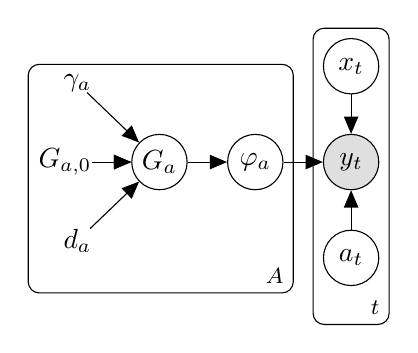
\begin{tikzpicture}
	% Nodes
	% Return y
	\node[obs] (y-t) {$y_{t}$};
	% Action a
	\node[latent, below=0.5 of y-t] (a-t) {$a_t$};
	% Context x
	\node[latent, above=0.5 of y-t]  (x-t) {$x_t$};
	% Nonparametric parameters
	\node[latent, left=0.5 of y-t, xshift=0cm] (varphi-a) {$\varphi_{a}$};
	% Nonparametric distribution
	\node[latent, left=0.5 of varphi-a, xshift=0cm] (G-a) {$G_{a}$};
	
	% Hyperparameters
	\node[const, left=0.5 of G-a, yshift=-1.0cm] (d-a) {$d_{a}$} ;
	\node[const, left=0.5 of G-a, yshift=0.0cm]  (G-a0) {$G_{a,0}$} ;
	\node[const, left=0.5 of G-a, yshift=1.0cm] (gamma-a) {$\gamma_{a}$} ;
	
	% Edges
	% Hyperparameters to distribution
	\edge {gamma-a,G-a0} {G-a} ;
	\edge {d-a,G-a0} {G-a} ;
	% Connect distribution to parameters
	\edge {G-a} {varphi-a} ;
	% Connect parameters, context and arm to observation
	\edge {varphi-a,x-t,a-t} {y-t} ;
	
	% Plates
	% Over time
	\plate {t} {(a-t)(x-t)(y-t)} {$t$} ;
	% Over each arm
	\plate {a}{
		(d-a)(gamma-a)(G-a0) % hyperparameters
		(G-a) % distribution
		(varphi-a) % parameters
	} {$A$} ;
\end{tikzpicture}
		\caption{The Bayesian nonparametric mixture bandit, as a probabilistic graphical model.}
		\label{fig:pgm_nonparametric_bandit}
		\vspace*{-4ex}
	\end{center}
\end{figure}

By characterizing each arm of the bandit with a different nonparametric model, we enjoy full flexibility to estimate each per-arm distribution independently, covering MAB cases with distinct reward model classes per-arm. This setting is a very powerful extension of the MAB problem, which has not attracted interest so far, yet can circumvent model misspecification.

At every interaction of the MAB agent with the environment, reward $y_{t,a_t}$ is \iid drawn from a context dependent unknown distribution $Y_{t,a_t}\sim p(Y|a_t,x_t,\thetastar)$ of the played arm $a_t$, which we here approximate via Bayesian nonparametric mixture models~\citep{b-Ghosal2017}.

Specifically, we model context-conditional reward densities with nonparametric Gaussian mixtures per-arm, \ie
\begin{align}
Y_{t,a} \sim p(Y|a,x_t,\varphi_a) &= \sum_{k=1}^{K_a} \frac{n_{a,k}-d_a}{n_a+\gamma_a} \cdot \N{Y|x_{t}^\top w_{a,k}, \sigma_{a,k}^2} \nonumber \\
& \qquad + \frac{\gamma_a+K_ad_a}{n_a+\gamma_a} \N{Y|x_{t}^\top w_{a,k_{new}}, \sigma_{a,k_{new}}^2} \;,
\label{eq:nonparametric_Gaussian_mixture}
\end{align}
where the number of mixands $K_a$ is determined by independent per-arm Pitman-Yor processes: $n_{a,k}$ refers to the rewards observed after playing arm $a$ that are assigned to mixture $k$, and $n_a=\sum_{k=1}^{K_a}n_{a,k}$.
After $n_{a}$ observations for arm $a$, there are $K_a$ already `\textit{seen}' mixtures, and a probability of $\frac{\gamma_a+K_ad_a}{n_a+\gamma_a}$ of incorporating a new mixand $k_{new}$ to the mixture.

Eqn.~\eqref{eq:nonparametric_Gaussian_mixture} describes per-arm nonparametric Gaussian mixture densities, with a Pitman-Yor nonparametric prior as described in Eqn.~\eqref{eq:pitman_yor_mixture}.
Each per-arm distribution is modeled independently with per-arm specific parameterizations: $d_a$, $\gamma_a$, $\varphi_{a,k}=\{w_{a,k}, \sigma_{a,k}^2 \}$, for $k={1,\cdots, K_a}$. 

The proposed contextual nonparametric model relies on leveraging context-conditional Gaussian models (with an expected value that is linearly dependent on the context at time $t$, \ie $\mu_{t,a,k}=x_t^\top w_{a,k}$), and extending them to a potentially infinite mixture.
As the number of mixands $K_a$ grows, the nonparametric distribution can be non-linear in the context.

With the proposed per-arm nonparametric mixture of Gaussian densities, we make a very flexible reward model assumption that automatically adjusts to the observed data: we are nonparametrically estimating complex, unknown per-arm continuous reward densities.
We leverage the well known linear Gaussian model and allow for the nonparametric model to accommodate as many mixands as necessary to best describe the observed bandit data.

The proposed Bayesian nonparametric model provides a flexible approach to density estimation, which can arbitrarily approximate continuous distributions. 
The Bayesian nonparametric literature has already established strong convergence results on the density estimation properties of these models: for a wide class of continuous distributions, the nonparametric posterior converges to the true data-generating density, under mild regularity conditions~\citep{j-Ghosal1999, j-Lijoi2004, j-Tokdar2006, j-Ghosal2007, j-Bhattacharya2010, j-Pati2013}.

In theory, the proposed Bayesian nonparametric model is on an infinite-dimensional parameter space (\ie the Pitman-Yor process can accommodate countably infinite mixands).
In practice, the model as in Eqn.~\eqref{eq:nonparametric_Gaussian_mixture} will use a finite subset of the available parameter dimensions to explain a finite sample of observations: \ie it sets the number of mixands per-arm $K_a$ according to the observed per-arm rewards.
Consequently, the effective complexity of the resulting model (\ie the dimensionality $K_a$ in Eqn.~\eqref{eq:nonparametric_Gaussian_mixture}) adapts to the observed data.

\subsection{Nonparametric context-conditional Gaussian mixture model posterior}
\label{ssec:nonparametric_posterior_update}

We now derive the procedure for inference of the per-arm, context-dependent reward posterior density of the proposed Bayesian nonparametric Gaussian mixture model.
As outlined in Section~\ref{ssec:background_nonparametric_mixture_model}, we rely on auxiliary latent variables per-arm $z_{1:n_a}$, and implement a Gibbs sampler that iterates between sampling mixture assignments $z_{1:n_a}$, and updating the emission distribution parameter posterior $G_{n_{a,k}}(\varphi_{a,k})$ for each arm and mixture. 

We start with the derivation of the parameter posteriors.
Per-arm and per-mixand emission distributions in Eqn.~\eqref{eq:nonparametric_Gaussian_mixture} are context-conditional Gaussian densities
\begin{equation}
\N{Y|x^\top w_{a,k}, \sigma_{a,k}^2} \; ,
\end{equation}
where $x^\top w_{a,k}$ and $\sigma_{a,k}^2$ are the means and variances, respectively, of the $k$-th mixand of arm $a$ in round $t$.
The conjugate prior of each of the mixands is a Normal-inverse Gamma,
\begin{equation}
G_{a,0}(\varphi_a) = \NIG{w_a, \sigma_a^2 |U_{a,0}, V_{a,0},\alpha_{a,0}, \beta_{a,0}} \;, 
\end{equation}
with hyperparameters $\varPhi_{a,0}=\{U_{a,0}, V_{a,0},\alpha_{a,0}, \beta_{a,0}\}$.

After observing rewards $y_{1:n}$, and conditioned on the auxiliary assignment variables $z_{1:n_a}$, the posteriors of per-arm and mixand parameters $\varphi_{a,k}$ follow a Normal-inverse Gamma distribution with updated hyperparameters $\varPhi_{a,k,n_{a,k}}$:
\begin{align}
G_{a,n_{a,k}}(\varphi_{a,k}) &=\NIG{w_{a,k}, \sigma_{a,k}^2 |\varPhi_{a,k,n_{a,k}}} \;, \\
\varPhi_{a,k,n_{a,k}}& =\{U_{a,k,n_{a,k}}, V_{a,k,n_{a,k}},\alpha_{a,k,n_{a,k}}, \beta_{a,k,n_{a,k}} \} \;, \nonumber
\end{align}
that depend on the number $n_{a,k}$ of rewards observed after playing arm $a$ that are assigned to mixand $k$. Specifically,
\begin{equation}
\begin{cases}
V_{a,k,n_{a,k}}^{-1} = x_{1:n} R_{a,k} x_{1:n}^\top + V_{a,0}^{-1} \;,\\
U_{a,k,n_{a,k}}= V_{a,k,n_{a,k}} \left( x_{1:n} R_{a,k} y_{1:n} + V_{a,0}^{-1} U_{a,0}\right) \;, \\
\alpha_{a,k,n_{a,k}} = \alpha_{a,0} + \frac{1}{2} \tr{R_{a,k}} \;, \\
\beta_{a,k,n_{a,k}} = \beta_{a,0} + \frac{1}{2}\left(y_{1:n}^\top R_{a,k}y_{1:n} \right) + \frac{1}{2}\left( U_{a,0}^\top V_{a,0}^{-1} U_{a,0} - U_{a,k,n_{a,k}}^\top V_{a,k,n_{a,k}}^{-1} U_{a,k,n_{a,k}} \right) \; ,
\end{cases}
\label{eq:posterior_hyperparameters}
\end{equation}
where $R_{a,k}\in\Real^{n_a\times n_a}$ is a sparse diagonal matrix with elements $\left[R_{a,k}\right]_{i,i}=\mathds{1}[a_i=a,z_i=k]$ for $i=\{0,\cdots, n_a\}$, and $n_{a}=\sum_{k=1}^{K_a} n_{a,k}$ is the number of rewards observed after playing arm $a$. The number of mixands per-arm $K_a$ of the bandit is independently drawn from its own Pitman-Yor process. Note that the above expression can be computed sequentially as data are observed for the played arm.

The predictive emission distribution after marginalization of the parameters $\varphi_{a,k}$, needed for solving Eqn.~\eqref{eq:gibbs_mixture_assignment}, follows a conditional Student-t distribution
\begin{align}
p_{a,k}(Y|a,x,\varPhi_{a,k,,n_{a,k}}) &= \T{Y|\nu_{a,k,n_{a,k}}, m_{a,k,n_{a,k}}, r_{a,k,n_{a,k}}} \;, \nonumber \\
\text{with } \varPhi_{a,k,,n_{a,k}} &=
\begin{cases}
\nu_{a,k,n_{a,k}}=2\alpha_{a,k} \;, \\
m_{a,k,n_{a,k}} = x^\top U_{a,k} \;, \\
r_{a,k,n_{a,k}}^2 = \frac{\beta_{a,k}}{\alpha_{a,k}} (1+x^\top V_{a,k} x) \;.
\end{cases}
\label{eq:marginalized_predictive_emission_univariate}
\end{align}
The hyperparameters $\varPhi_{a,k,,n_{a,k}}=\{\nu_{a,k,n_{a,k}}, m_{a,k,n_{a,k}}, r_{a,k,n_{a,k}}\}$ above are those of the prior $\varPhi_{a,0}$, or the posterior $\varPhi_{a,k,n_{a,k}}$, depending on whether the predictive density refers to a `\textit{new}' mixand $k_{new}$ with $n_{a,k=k_{new}}=0$, or a `\textit{seen}' mixand $k$, for which $n_{a,k}\geq0$ observations have been already assigned to, respectively.

Similarly, the likelihood of a set of rewards assigned to per-arm mixand $k$, $Y_{a,k}=y_{1:n}\cdot \mathds{1}[a_n=a,z_n=k]$, given their associated contexts $X_{a,k}=x_{1:n} \cdot \mathds{1}[a_n=a,z_n=k]$, follows the matrix t-distribution
\begin{align}
&p(Y_{a,k}|X_{a,k},X_{\backslash a,k},Y_{\backslash a,k},\varPhi_{a,k}) = \MT{Y_{a,k}|\nu_{Y_{a,k}}, M_{Y_{a,k}}, \Psi_{Y_{a,k}}, \Omega_{Y_{a,k}}} \; , \nonumber  \\
\text{with }&\begin{cases}
\nu_{Y_{a,k}}=2 \alpha_{a,k} \;,\\
M_{Y_{a,k}}= X_{a,k}^\top U_{a,k} \;, \\
\Psi_{Y_{a,k}} = I_{n_{a,k}} + X_{a,k}^\top V_{a,k} X_{n_{a,k}} \;,\
\Omega_{Y_{a,k}} = 2 \beta_{a,k} \;.
\end{cases}
\label{eq:marginalized_predictive_emission_multivariate}
\end{align}

With parameter posteriors as in Eqns.~\eqref{eq:marginalized_predictive_emission_univariate} and~\eqref{eq:marginalized_predictive_emission_multivariate}, we implement a Gibbs sampler to infer the mixture assignments $z_{1:n}$, based on the assignment probabilities described in Eqn.~\eqref{eq:gibbs_mixture_assignment}, for per-arm already drawn mixture components $k_a\in\{1, \cdots, K_a\}$, and a new `\textit{unseen}' mixand $k_{a,new}$. Therefore, the proposed Gibbs sampler adjusts the nonparametric posterior's complexity (\ie number of mixands $K_a$) according to the observed per-arm rewards distribution.

\subsection{Nonparametric Gaussian mixture model based Thompson sampling}
\label{ssec:nonparametric_thompson_sampling}

We leverage the nonparametric context-conditional Gaussian mixture model described above, and combine it with a posterior sampling MAB policy, \ie Thompson sampling~\citep{j-Russo2018}. The proposed Thompson sampling technique for contextual bandits with nonparametric Gaussian mixture reward models is presented in Algorithm~\ref{alg:nonparametric_ts}.

%Nonparametric TS
\vspace*{-2ex}
\begin{algorithm}
	\caption{Nonparametric Gaussian mixture model based Thompson sampling}
	\label{alg:nonparametric_ts}
	\begin{algorithmic}[1]
		\STATE {\bfseries Input:} Number of arms $|\A|$
		\STATE {\bfseries Input:} Per-arm hyperparameters $d_a$, $\gamma_a$, $\varPhi_{a,0}$
		\STATE {\bfseries Input:} Gibbs convergence criteria $\epsilon$, $Gibbs_{max}$ 
		\STATE $\HH_1=\emptyset$
		\FOR{$t=1, \cdots, T$}
		\STATE Receive context $x_{t}$
		\FOR{$a=1, \cdots, |\A|$}
		\STATE Draw parameters from the posterior \\ $\hspace*{2ex}\varphi_{a,k}^{(t)} \sim G_{a,k,n_{a,k}}(\varPhi_{a,k}), \forall k$, as in Eqn.~\eqref{eq:posterior_hyperparameters}
		\STATE Compute $\mu_{t,a}(x_{t},\varphi_{a}^{(t)})$ as in Eqn.~\eqref{eq:nonparametric_expected_reward}
		\ENDFOR
		\STATE Play arm $a_{t}=\argmax_{a^\prime \in \A} \mu_{t,a^\prime}(x_{t},\varphi_{a^\prime}^{(t)})$
		\STATE Observe reward $y_{t}$
		\STATE $\HH_{1:t}=\HH_{1:t-1} \cup \left\{x_{t}, a_{t}, y_{t}\right\}$
		\WHILE{NOT Gibbs convergence criteria}
		\STATE Update mixture assignments $z_{1:n}$ based on Eqn.~\eqref{eq:gibbs_mixture_assignment}
		\STATE Compute sufficient statistics $n_{a,k}$
		\STATE Update parameter posteriors $\varPhi_{a,k,n_{a,k}}$ based on Eqn.~\eqref{eq:posterior_hyperparameters}
		\ENDWHILE
		\ENDFOR
	\end{algorithmic}
\end{algorithm}
\vspace*{-2ex}

At each interaction with the world, the proposed Thompson sampling decides which arm to play next based on a random parameter sample, drawn from the posterior nonparametric distribution updated with all the information available at time $t$.

The parameters' posterior distributions for the proposed nonparametric Gaussian mixture model are presented in Section~\ref{ssec:nonparametric_posterior_update}.
Specifically, for nonparametric models as in Eqn~\eqref{eq:nonparametric_Gaussian_mixture}, one draws per-arm and per-mixand Gaussian parameters $\varphi_{a,k}$ from the posterior distributions with updated hyperparameters $\varPhi_{a,k,n_{a,k}}$ in Eqn.~\eqref{eq:posterior_hyperparameters}, conditioned on the mixture assignments $z_{1:n}$ determined by the Gibbs sampler in Eqn.~\eqref{eq:gibbs_mixture_assignment}, with marginalized emission densities provided in Eqns.~\eqref{eq:marginalized_predictive_emission_univariate} and~\eqref{eq:marginalized_predictive_emission_multivariate}.

Given the inferred sufficient statistics of the assignments (\ie the counts $n_{a,k}$ of rewards observed for arm $a$ and assigned to mixand $k$), and the drawn posterior parameter samples $w_{a,k}^{(t)}$, one computes the expected reward for each arm of the nonparametric bandit, \ie

\begin{align}
\mu_{t,a}(x_{t},\varphi_{a}^{(t)})&=\sum_{k=1}^{K_a} \frac{n_{a,k}-d_a}{n_a+\gamma_a} \left(x_{t}^\top w_{a,k}^{(t)}\right) + \frac{\gamma_a+K_ad_a}{n_a+\gamma_a} \left(x_{t}^\top w_{a,k_{new}}^{(t)} \right)\; .
\label{eq:nonparametric_expected_reward}
\end{align}

The proposed Thompson sampling policy $\myPitilde{\Atilde_t|x_{t},\HH_{1:t-1}}$, with assumed per-arm nonparametric distribution $\ptilde(Y|a,x_t,\varphi_a)$ in Eqn~\eqref{eq:nonparametric_Gaussian_mixture}, picks the arm that maximizes the above expected reward, \ie
\begin{align}
\myPitilde{\Atilde_t|x_{t},\HH_{1:t-1}}&=\myPitilde{\Atilde_t|x_{t},\varphi_{a}^{(t)}} \nonumber \\
& =\myind{\Atilde_t=\argmax_{a^\prime \in \A} \mu_{t,a}\left(x_{t},\varphi_{a}^{(t)}\right)}\;, \varphi_{a}^{(t)} \sim p(\varphi_{a}|\HH_{1:t-1}) \;,
\end{align}
with updated hyperparameters for $\ptilde(\varphi_{a}|\HH_{1:t-1})$ as in Eqn.~\eqref{eq:posterior_hyperparameters}.

\subsubsection{Regret bound}
\label{sssec:nonparametric_thompson_sampling_regret_bound}

We leverage asymptotic posterior converge rates ---the rate at which the distance between two densities becomes small as the number of observation grows--- to asymptotically bound the regret of the proposed nonparametric Thompson sampling algorithm.

A Thompson sampling-based policy operates according to the probability of each arm being optimal. This probability is equivalent to the expectation with respect to the joint posterior distribution of the expected rewards given history and context, $p(\mu_t|x_{t},\HH_{1:t-1})$, of the optimal arm indicator function, \ie
\begin{align}
\myPi{p}{A_t|x_{t},\HH_{1:t-1}} &= \myProb{p}{A_t=\argmax_{a^\prime \in \A} \mu_{t,a^\prime}} =\eValue{p}{\myind{A_t=\argmax_{a^\prime \in \A}\mu_{t,a^\prime}}} \;.
\nonumber
\end{align}

Note that the indicator function $\myind{A_t=\argmax_{a^\prime \in \A}\mu_{t,a^\prime}}$ for each arm requires the posterior over all arms $a^\prime \in \A$ as input. That is, the posterior $p(\mu_t|x_{t},\HH_{1:t-1})$ is the joint posterior distribution over the expected rewards of all arms: $\mu_{t}=\{\mu_{t,a}\}, \forall a\in \A$; \ie it is a $|\A|$ dimensional multivariate distribution over all arms of the bandit.

We now present our first lemma, with the proof provided in Section~\ref{asec:nonparametric_thompson_sampling_regret_bound} of the Appendix, which is key to the cumulative regret theorem that follows.
\begin{lemma}
	The difference in action probabilities between two Thompson sampling policies, given the same history and context up to time $t$, is bounded by the total-variation distance $\delta_{TV}(p_t,q_t)$ between the posterior distributions of their expected rewards at time $t$, $p_t=p(\mu_{t}|x_t,\HH_{1:t-1})$ and $q_t=q(\mu_{t}|x_t,\HH_{1:t-1})$, respectively,
	\begin{equation}
	\myPi{p_t}{A_t=a} - \myPi{q_t}{A_t=a} \leq \delta_{TV}(p_t,q_t) \; .
	\nonumber
	\end{equation}
	\label{lemma:total_variation_bounds_diff_policies}
	The \textbf{total variation distance} $\delta_{TV}(p,q)$ between distributions $p$ and $q$ on a sigma-algebra $\mathcal{F}$ of subsets of the sample space $\Omega$ is defined as
	\begin{equation}
	\delta_{TV}(p, q) = \sup_{B \in \mathcal{F}} \left|p(B)-q(B)\right| \; ,
	\end{equation}
	which is properly defined for both discrete and continuous distributions (see details in Section~\ref{asec:nonparametric_thompson_sampling_regret_bound} of the Appendix).
\end{lemma}
We make use of Lemma~\ref{lemma:total_variation_bounds_diff_policies} to asymptotically bound the cumulative regret of the proposed Thompson sampling with Dirichlet process priors (\ie $d_a=0, \forall a$) and Gaussian emission distributions, for bandits with true reward densities that meet certain regularity conditions. 

\begin{theorem}
	The expected cumulative regret at time $T$ of a Dirichlet process Gaussian mixture model based Thompson sampling algorithm is asymptotically bounded by
	\begin{equation}
	R_T	\leq \mathcal{O}\left(|\A| \log^\kappa T \sqrt{T} \right) \; \text{ as } T \rightarrow \infty \; .
	\nonumber
	\end{equation}
	We use big-O notation $\mathcal{O}(\cdot)$ for the asymptotic regret bound, as it bounds from above the growth of the cumulative regret over time for large enough bandit interactions, \ie
	\begin{align}
	\lim_{T\rightarrow \infty} \frac{R_T}{|\A| \log^\kappa T \sqrt{T} } & \leq \mathcal{O}(1)\; .
	\end{align}
	We note that this bound holds both in a frequentist and Bayesian view of expected regret.
	\label{th:regret_bound}
\end{theorem}

The proof of Theorem~\ref{th:regret_bound}, provided in Section~\ref{asec:nonparametric_thompson_sampling_regret_bound} of the Appendix, consists of bounding the regret introduced by two factors: the first, related to the use of Thompson sampling (\ie a policy that does not know the true parameters of the reward distribution, but has knowledge of the true reward model class); and the second, a term that accounts for the convergence of the posterior of a nonparametric model to that of the true data generating distribution.

The logarithmic term $\log^\kappa T$ in the bound appears due to the convergence rate of the nonparametric density estimation, where the exponent $\kappa\geq 0$ depends on the tail behavior of the base measure and the priors of the Dirichlet process ---see Section \ref{asec:nonparametric_thompson_sampling_regret_bound} of the Appendix, and references therein, for details on density convergence and its impact on the exponent $\kappa\geq 0$.

\subsubsection{Computational complexity}
\label{sssec:nonparametric_thompson_sampling_computational_complexity}
The Gibbs sampler in the proposed nonparametric Thompson sampling (lines 14-18 within Algorithm~\ref{alg:nonparametric_ts}) is run $Gibbs_{steps}$ until a stopping criteria is met: either the model likelihood of the sampled chain is stable within an $\epsilon$ likelihood margin between steps, or a maximum number of iterations $Gibbs_{max}$ is reached.

As new rewards $y_{t,a_{t}}$ are acquired, updates to assignments $z_{t^\prime,a_{t}}$ are computed sequentially within the Gibbs sampler for $t^\prime=\{1,\cdots,t | a_{t^\prime}=a_{t}\}$; \ie only the posterior over the last played armed $a_{t}$ is recomputed. Since Eqn.~\eqref{eq:posterior_hyperparameters} can be sequentially computed for each per-arm observation, the computational cost of the Gibbs sampler grows with the number of available observation of the played arm. Therefore, the overall computational cost is upper-bounded by $\mathcal{O}(T \cdot Gibbs_{steps})$ per-interaction with the world, \ie per newly observed reward $y_{t,a_{t}}$.

Due to the sequential acquisition of observations in the bandit setting, and the need to only update the posterior for the played arm, the Gibbs sampler is \textit{warm-started} at each bandit interaction, and good convergence can be achieved in few iterations per observed reward. 
In practice, and because of the \textit{warm-start}, one can limit the number of Gibbs sampler iterations per-bandit interaction to upper-bound the algorithm's complexity to $O(T\cdot Gibbs_{max})$ per interaction, yet achieve satisfactory performance ---empirical evidence of this claim is provided in Section~\ref{sssec:evaluation_mixture_scenarios_baselines}.
Due to the \textit{warm-start}, the Gibbs sampler is run from a good starting point: the per-arm parameter space that describes all but this newly observed reward $y_{t,a_{t}}$.

We emphasize that we propose a Gibbs sampler that runs until convergence, but suggest to limit the number of Gibbs iterations as a practical recommendation with good empirical regret performance, yet upper-bounded $\mathcal{O}(T \cdot Gibbs_{max})$ computational complexity per MAB interaction with the environment.


\section{Evaluation}
\label{sec:evaluation}
% !TEX root = smc_bandits.tex
We empirically evaluate the proposed SMC-based Bayesian MAB framework
in non-stationary bandit scenarios
%\footnote{
%	Results in Appendix~\ref{assec:static_bandits_experiments_analytical}
%	validate the performance of SMC-based policies in stationary bandits.
%	We compare their performance to solutions based on analytically attainable posteriors
%	with Bernoulli and contextual linear Gaussian reward functions~\citep{ip-Kaufmann2012,ip-Garivier2011a,ic-Korda2013,ip-Agrawal2013a},
%	as well as for context-dependent binary rewards modeled with the logistic reward function~\cite{ic-Chapelle2011,j-Scott2015} ---Appendix~\ref{assec:static_bandits_experiments_logistic}.
%	Results showcase satisfactory performance across a wide range of stationary bandit parameterizations and sizes,
%	as SMC-based policies achieve the right exploration-exploitation tradeoff.
%}
with continuous, binary and discrete-categorical reward distributions.

Results in Appendix~\ref{assec:static_bandits_experiments_analytical}
validate the performance of SMC-based policies in stationary bandits.
We compare their performance to solutions based on analytically attainable posteriors
with Bernoulli and contextual linear Gaussian reward functions~\citep{ip-Kaufmann2012,ip-Garivier2011a,ic-Korda2013,ip-Agrawal2013a},
as well as for context-dependent binary rewards modeled with the logistic reward function~\cite{ic-Chapelle2011,j-Scott2015} ---Appendix~\ref{assec:static_bandits_experiments_logistic}.
Results showcase satisfactory performance across a wide range of stationary bandit parameterizations and sizes,
as SMC-based policies achieve the right exploration-exploitation tradeoff.

For results we present below, we simulate different parameterizations of dynamic linear models described in Section~\ref{ssec:linear_mixing_dynamics},
and present results for a variety of MAB environments with reward functions detailed in Sections~\ref{ssec:dynamic_bandits_gaussian},~\ref{ssec:dynamic_bandits_logistic} and~\ref{ssec:dynamic_bandits_categorical}.
Section~\ref{ssec:logged_data_bandits} illustrates
the ability of SMC-based bandit policies
to capture non-stationary trends in personalized news article recommendations.

The main evaluation metric is the cumulative regret of the bandit agent, as defined in Equation~\eqref{eq:mab_cumulative_regret},
with results averaged over 500 realizations.
We present results for SMC-based policies with $M=2000$ samples,
and provide an evaluation of the impact of $M$ in Appendix~\ref{asec:dynamic_bandits}.

\subsection{Non-stationary, linear Gaussian rewards}
\label{ssec:dynamic_bandits_gaussian}
% !TEX root = smc_bandits.tex
We simulate the following two-armed, contextual ($x_t\in\Real^2, \forall t$), linear Gaussian bandit:
\begin{equation}
\text{Scenario A}
\begin{cases}
	\vspace*{1ex}
	p(\theta_{t,a=0}|\theta_{t-1,a=0}): \\ \vspace*{1ex}
	\hspace*{10ex}\begin{pmatrix}
	\theta_{t,a=0,0}\\
	\theta_{t,a=0,1}\\
	\end{pmatrix} = \begin{pmatrix}
	0.9 & -0.1 \\
	-0.1 & 0.9 \\
	\end{pmatrix} \begin{pmatrix}
	\theta_{t-1,a=0,0}\\
	\theta_{t-1,a=0,1}\\
	\end{pmatrix} + \epsilon_{a=0} \;, \\ \vspace*{1ex}
	\hspace*{40ex} \text{where } \;  \epsilon_{a=0} \sim \N{\epsilon|0,0.01 \cdot\mathrm{I}},\\
	
	\vspace*{1ex}
	p(\theta_{t,a=1}|\theta_{t-1,a=1}): \\ \vspace*{1ex}
	\hspace*{10ex}\begin{pmatrix}
	\theta_{t,a=1,0}\\
	\theta_{t,a=1,1}\\
	\end{pmatrix} = \begin{pmatrix}
	0.9 & 0.1 \\
	0.1 & 0.9 \\
	\end{pmatrix} \begin{pmatrix}
	\theta_{t-1,a=1,0}\\
	\theta_{t-1,a=1,1}\\
	\end{pmatrix} + \epsilon_{a=1} \;, \\ \vspace*{1ex}
	\hspace*{40ex} \text{where } \;  \epsilon_{a=1} \sim \N{\epsilon|0,0.01 \cdot\mathrm{I}},\\
	
	p_a(Y|x,\theta_{t,a})=\N{Y|x^\top \theta_{t,a}, \sigma_a^2} \;.
\end{cases}
\label{eq:linear_mixing_dynamics_a}
\end{equation}

\begin{equation}
\text{Scenario B}
\begin{cases}
	\vspace*{1ex}
	p(\theta_{t,a=0}|\theta_{t-1,a=0}): \\ \vspace*{1ex}
	\hspace*{10ex}\begin{pmatrix}
	\theta_{t,a=0,0}\\
	\theta_{t,a=0,1}\\
	\end{pmatrix} = \begin{pmatrix}
	0.5 & 0.0 \\
	0.0 & 0.5 \\
	\end{pmatrix} \begin{pmatrix}
	\theta_{t-1,a=0,0}\\
	\theta_{t-1,a=0,1}\\
	\end{pmatrix} + \epsilon_{a=0} \;, \\ \vspace*{1ex}
	\hspace*{40ex} \text{where } \;  \epsilon_{a=0} \sim \N{\epsilon|0,0.01 \cdot\mathrm{I}},\\
	
	\vspace*{1ex}
	p(\theta_{t,a=1}|\theta_{t-1,a=1}): \\ \vspace*{1ex}
	\hspace*{10ex}\begin{pmatrix}
	\theta_{t,a=1,0}\\
	\theta_{t,a=1,1}\\
	\end{pmatrix} = \begin{pmatrix}
	0.9 & 0.1 \\
	0.1 & 0.9 \\
	\end{pmatrix} \begin{pmatrix}
	\theta_{t-1,a=1,0}\\
	\theta_{t-1,a=1,1}\\
	\end{pmatrix} + \epsilon_{a=1} \;, \\ \vspace*{1ex}
	\hspace*{40ex} \text{where } \;  \epsilon_{a=1} \sim \N{\epsilon|0,0.01 \cdot\mathrm{I}}, \\
	
	p_a(Y|x,\theta_{t,a})=\N{Y|x^\top \theta_{t,a}, \sigma_a^2} \;.
\end{cases}
\label{eq:linear_mixing_dynamics_b}
\end{equation}
 
The expected rewards driven by the dynamics of Equations~\eqref{eq:linear_mixing_dynamics_a} and~\eqref{eq:linear_mixing_dynamics_b} change over time,
inducing switches on the identity of the optimal arm.
%
For instance, for a given realization of Scenario A shown in Figure~\ref{fig:linear_mixing_dynamics_a_gaussian},
there is an optimal arm swap between time-instants $t=(300, 550)$, with arm 1 becoming the optimal for all $t\geq600$;
for a realization of Scenario B illustrated in Figure~\ref{fig:linear_mixing_dynamics_b_gaussian},
there is an optimal arm change around $t=100$, a swap around $t=600$,
with arm 1 becoming optimal again after $t\geq1600$.

Empirical results for SMC-based Bayesian policies in scenarios described by Equations~\eqref{eq:linear_mixing_dynamics_a} and~\eqref{eq:linear_mixing_dynamics_b}
are shown in Figures~\ref{fig:dynamic_bandits_linearGaussian_dknown} and \ref{fig:dynamic_bandits_linearGaussian_dunknown}.

% Linear Gaussian, known parameters
\begin{figure}[!h]
	\centering
	\begin{subfigure}[b]{0.45\textwidth}
		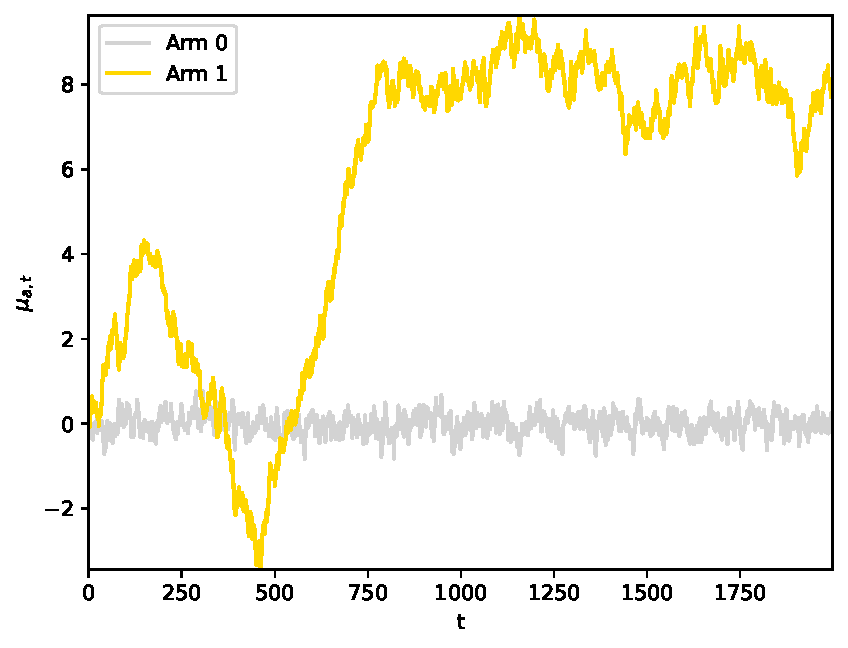
\includegraphics[width=\textwidth]{./fods_figs/dynamic/linearGaussian/dynamics_a}
		\caption{Expected per-arm rewards over time for Scenario A in Equation~\eqref{eq:linear_mixing_dynamics_a}.}
		\label{fig:linear_mixing_dynamics_a_gaussian}
	\end{subfigure}\qquad
	\begin{subfigure}[b]{0.45\textwidth}
		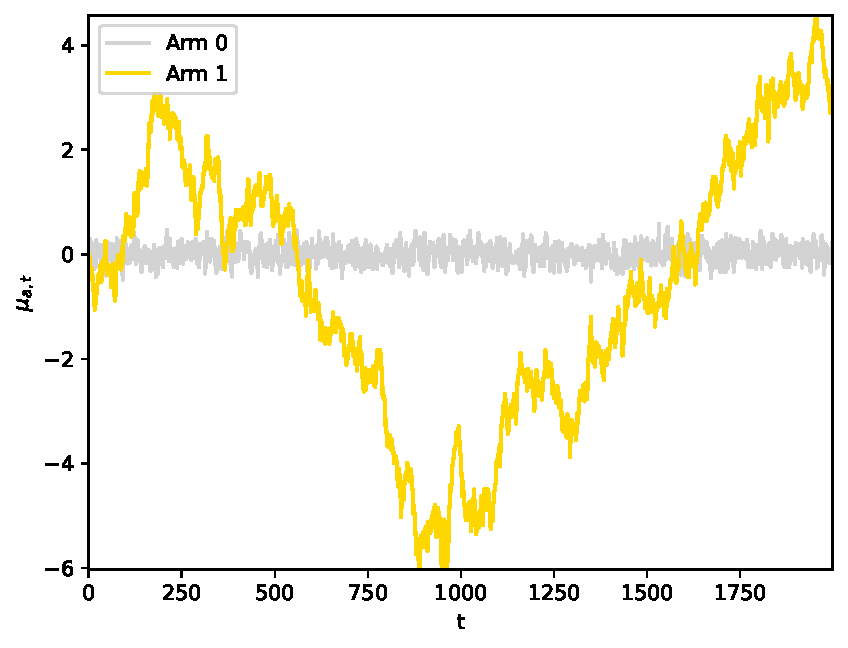
\includegraphics[width=\textwidth]{./fods_figs/dynamic/linearGaussian/dynamics_b}
		\caption{Expected per-arm rewards over time for Scenario B in Equation~\eqref{eq:linear_mixing_dynamics_a}.}
		\label{fig:linear_mixing_dynamics_b_gaussian}
	\end{subfigure}
	
	\begin{subfigure}[b]{0.47\textwidth}
		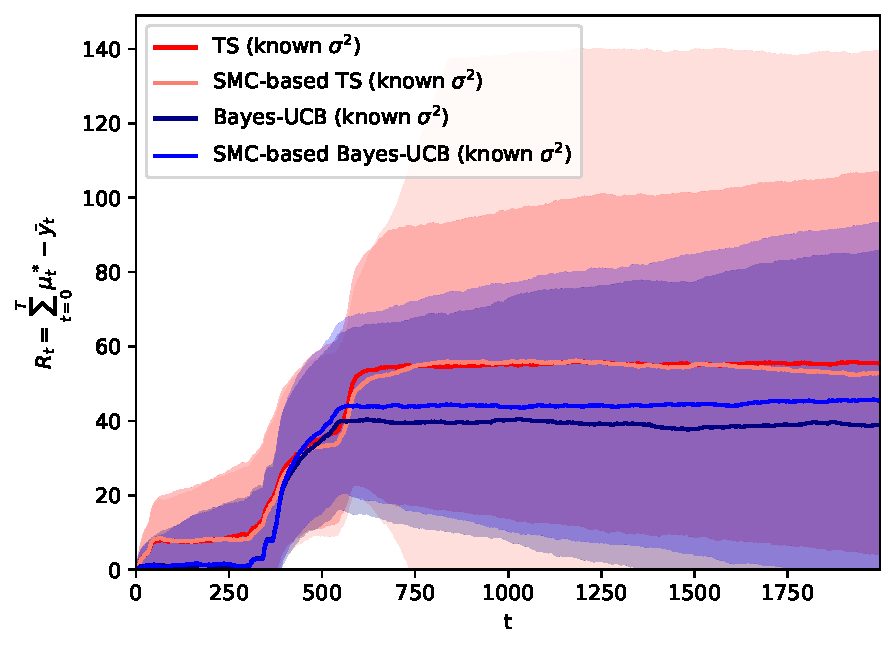
\includegraphics[width=\textwidth]{./fods_figs/dynamic/linearGaussian/a_M2000_cumulative_regret_dknown_knownsigma}
		\caption{Cumulative regret for SMC-based Bayesian policies in scenario A: known dynamic parameters.}
		\label{fig:dynamic_bandits_linearGaussian_a_cstatic_dknown_knownsigma}
	\end{subfigure}\qquad
	\begin{subfigure}[b]{0.47\textwidth}
		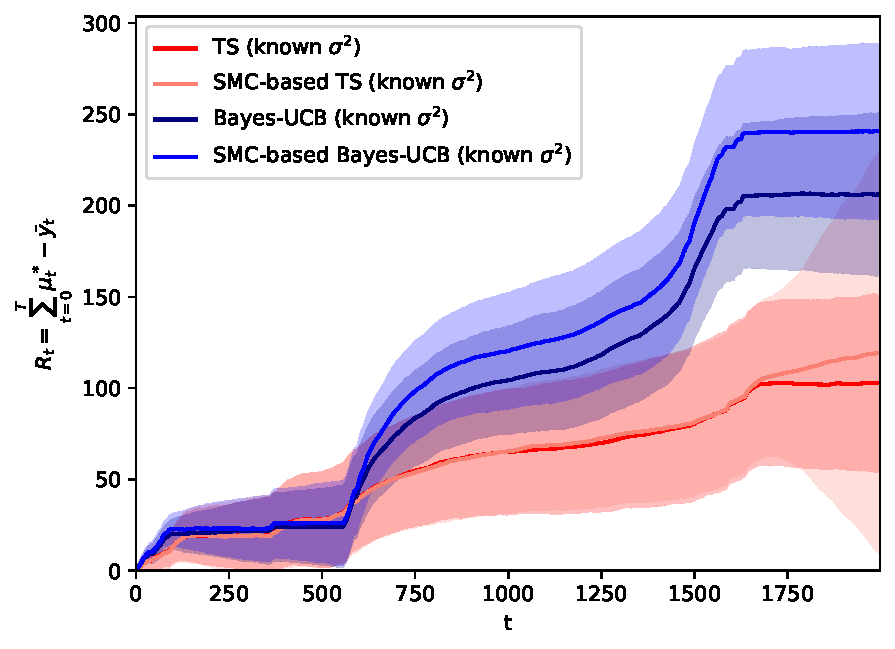
\includegraphics[width=\textwidth]{./fods_figs/dynamic/linearGaussian/b_M2000_cumulative_regret_dknown_knownsigma}
		\caption{Cumulative regret for SMC-based Bayesian policies in scenario B: known dynamic parameters.}
		\label{fig:dynamic_bandits_linearGaussian_b_cstatic_dknown_knownsigma}
	\end{subfigure}
	
	\caption{
		Mean regret (standard deviation shown as shaded region) in contextual, linear Gaussian bandit Scenarios A and B
		described in Equations~\eqref{eq:linear_mixing_dynamics_a}--\eqref{eq:linear_mixing_dynamics_b},
		when the bandit agent knows the latent dynamic parameterization.
		Notice how
		in Figures~\ref{fig:dynamic_bandits_linearGaussian_a_cstatic_dknown_knownsigma}--\ref{fig:dynamic_bandits_linearGaussian_b_cstatic_dknown_knownsigma}
		regret increases when the optimal arms swap
		(as shown in Figures~\ref{fig:linear_mixing_dynamics_a_gaussian}--\ref{fig:linear_mixing_dynamics_b_gaussian}).
		SMC-based policies successfully find the right exploration-exploitation tradeoff,
		with minimal additional regret incurred in comparison to their analytical alternatives. 
	}
	\label{fig:dynamic_bandits_linearGaussian_dknown}
\end{figure}

We study linear dynamics with Gaussian reward distributions with known parameters in Figure~\ref{fig:dynamic_bandits_linearGaussian_dknown},
of interest as it allows us to validate the SMC-based random measure in comparison to the optimal, closed-form posterior
---the Kalman filter~\cite{j-Kalman1960}---
under the assumption of known dynamic parameters.

We observe satisfactory cumulative regret performance in Figure~\ref{fig:dynamic_bandits_linearGaussian_dknown}:
\ie SMC-based Bayesian agents' cumulative regret is sublinear.
Policies that compute and use SMC random measure posteriors
incur in minimal regret loss 
in comparison to the optimal Kalman filter-based agent.
Namely, the shape of the regret curves of \textit{TS} and \textit{SMC-based TS}
(\textit{Bayes-UCB} and \textit{SMC based Bayes-UCB}, respectively) in Figure~\ref{fig:dynamic_bandits_linearGaussian_dknown} is equivalent,
with minimal differences in average cumulative regret when compared to the volatility across realizations.
Importantly, all policies are able to adapt to the changes over time of the identify of the optimal arm. 

We illustrate in Figure~\ref{fig:dynamic_bandits_linearGaussian_dunknown}
a more realistic scenario, where the dynamic parameterization is unknown to the bandit agent.

We observe in Figures~\ref{fig:dynamic_bandits_linearGaussian_a_cstatic_dknown_unknownsigma}--\ref{fig:dynamic_bandits_linearGaussian_b_cstatic_dknown_unknownsigma} that,
in the case of unknown reward variances ($\sigma_a^2, \forall a)$,
SMC-based policies perform comparably well.
In these cases,
the agents' reward model is not Gaussian,
but Student-t distributed, as per the marginalized posterior in Equation~\eqref{eq:t_posterior_mean}.
The regret loss associated with the uncertainty about $\sigma_a^2$ is minimal for SMC-based Bayesian agents,
and does not hinder the ability of the proposed SMC-based policies
to find the right exploration-exploitation balance:
\ie regret is sublinear, and the agents adapt to switches in the identity of the optimal arm.

We illustrate in Figures~\ref{fig:dynamic_bandits_linearGaussian_a_cstatic_dunknown}--\ref{fig:dynamic_bandits_linearGaussian_b_cstatic_dunknown}
the most realistic, yet challenging, non-stationary contextual Gaussian bandit case:
one where none of the parameters of the model are known.
In this case, the agent must sequentially learn both the underlying dynamics ($L_a,\Sigma_a; \forall a$)
and the conditional reward function's variance ($\sigma_a^2, \forall a)$,
in order to infer the posterior distribution over the latent, time-varying sufficient statistics of interest,
to enable informed sequential decision making.

Cumulative regret results in Figures~\ref{fig:dynamic_bandits_linearGaussian_a_cstatic_dunknown}--\ref{fig:dynamic_bandits_linearGaussian_b_cstatic_dunknown}
showcase a regret performance loss due to the need to learn all these unknown parameters.
We observe noticeable (almost linear) regret increases when the dynamics of the parameters swap the identity of the optimal arm.
However, SMC-based Thompson sampling and Bayes-UCB agents are able to learn the evolution of the dynamic latent parameters,
and the corresponding time-varying expected rewards,
with enough accuracy to attain good exploration-exploitation balance:
\ie sublinear regret curves indicate the agent identified and played the optimal arm repeatedly.
Figure~\ref{fig:dynamic_bandits_linearGaussian_a_cstatic_dunknown} is clear evidence of the SMC-based agents' ability to recover from linear to no-regret regimes.

\begin{figure}[!h]
	\centering
	\begin{subfigure}[b]{0.45\textwidth}
		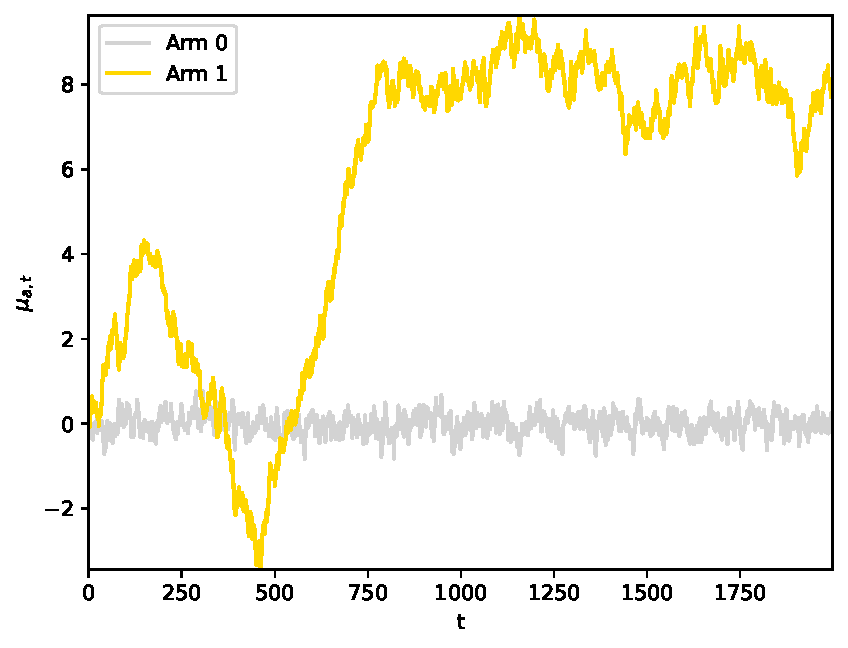
\includegraphics[width=\textwidth]{./fods_figs/dynamic/linearGaussian/dynamics_a}
		\caption{Expected per-arm rewards over time for Scenario A in Equation~\eqref{eq:linear_mixing_dynamics_a}.}
		\label{fig:linear_mixing_dynamics_a_gaussian_2}
	\end{subfigure}\qquad
	\begin{subfigure}[b]{0.45\textwidth}
		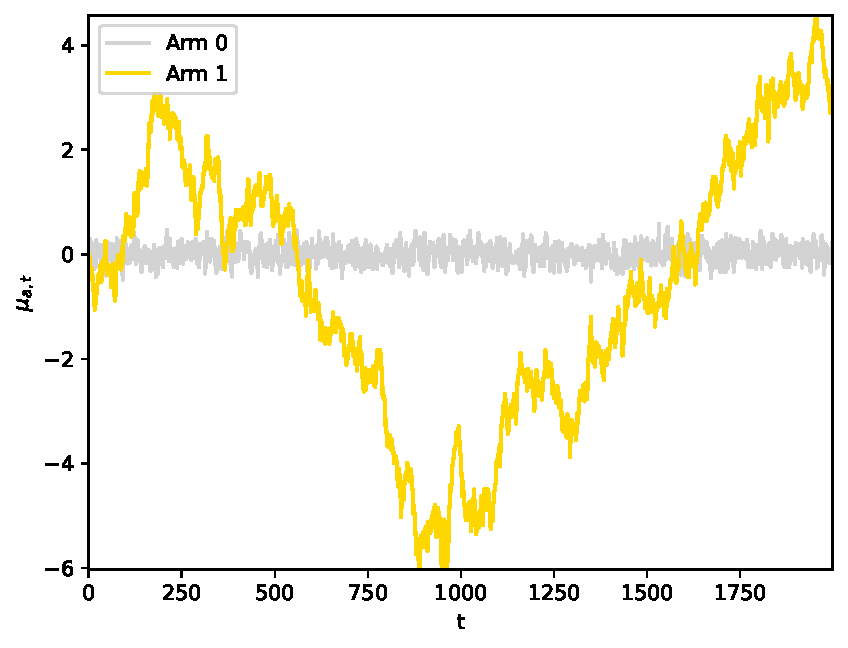
\includegraphics[width=\textwidth]{./fods_figs/dynamic/linearGaussian/dynamics_b}
		\caption{Expected per-arm rewards over time for Scenario B in Equation~\eqref{eq:linear_mixing_dynamics_a}.}
		\label{fig:linear_mixing_dynamics_b_gaussian_2}
	\end{subfigure}
	
	\begin{subfigure}[b]{0.47\textwidth}
		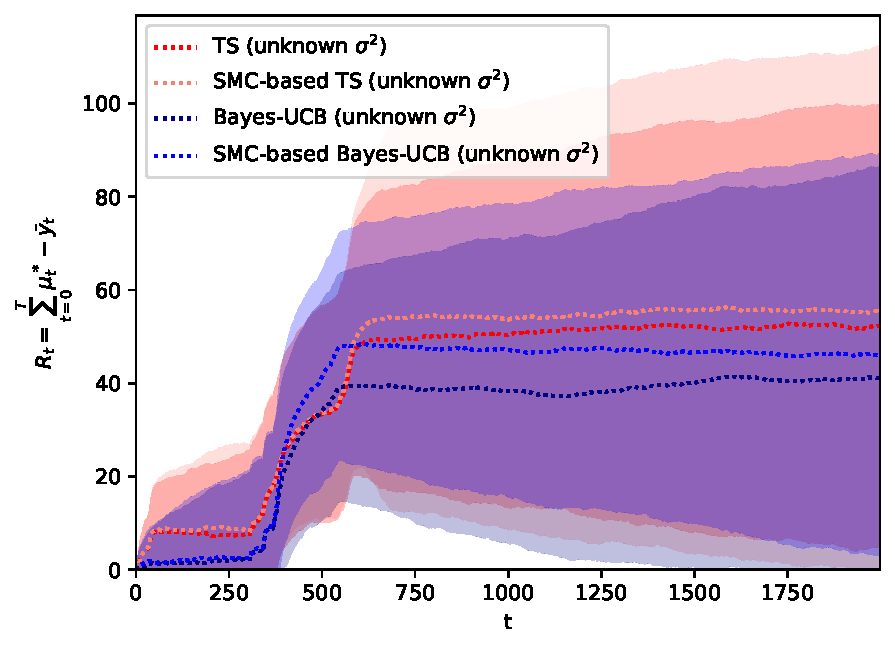
\includegraphics[width=\textwidth]{./fods_figs/dynamic/linearGaussian/a_M2000_cumulative_regret_dknown_unknownsigma}
		\caption{Cumulative regret for SMC-based Bayesian policies in scenario A: known dynamic parameters, unknown $\sigma_a, \forall a$.}
		\label{fig:dynamic_bandits_linearGaussian_a_cstatic_dknown_unknownsigma}
	\end{subfigure}\qquad
	\begin{subfigure}[b]{0.47\textwidth}
		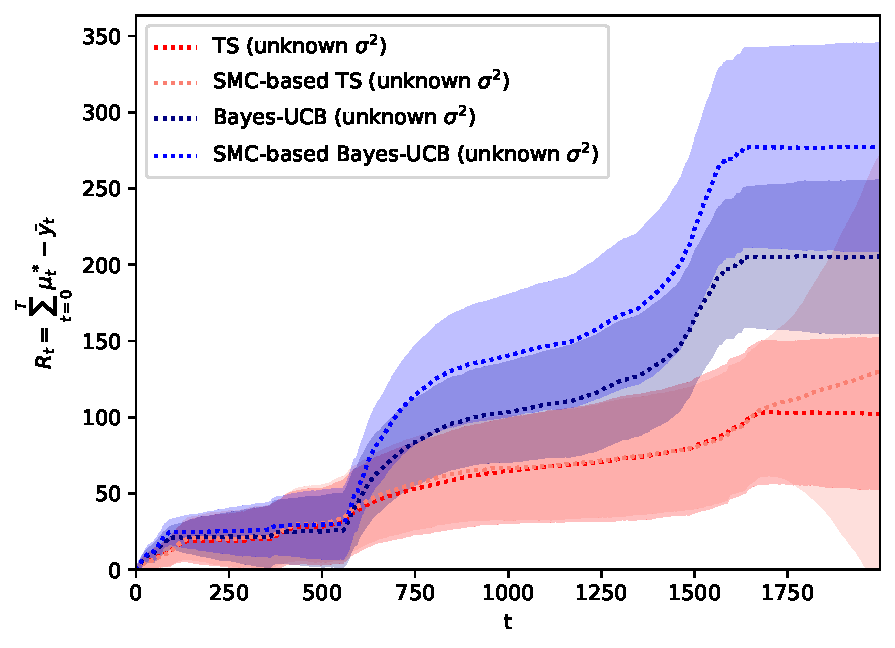
\includegraphics[width=\textwidth]{./fods_figs/dynamic/linearGaussian/b_M2000_cumulative_regret_dknown_unknownsigma}
		\caption{Cumulative regret for SMC-based Bayesian policies in scenario B: known dynamic parameters, unknown $\sigma_a, \forall a$.}
		\label{fig:dynamic_bandits_linearGaussian_b_cstatic_dknown_unknownsigma}
	\end{subfigure}
	
	\begin{subfigure}[b]{0.47\textwidth}
		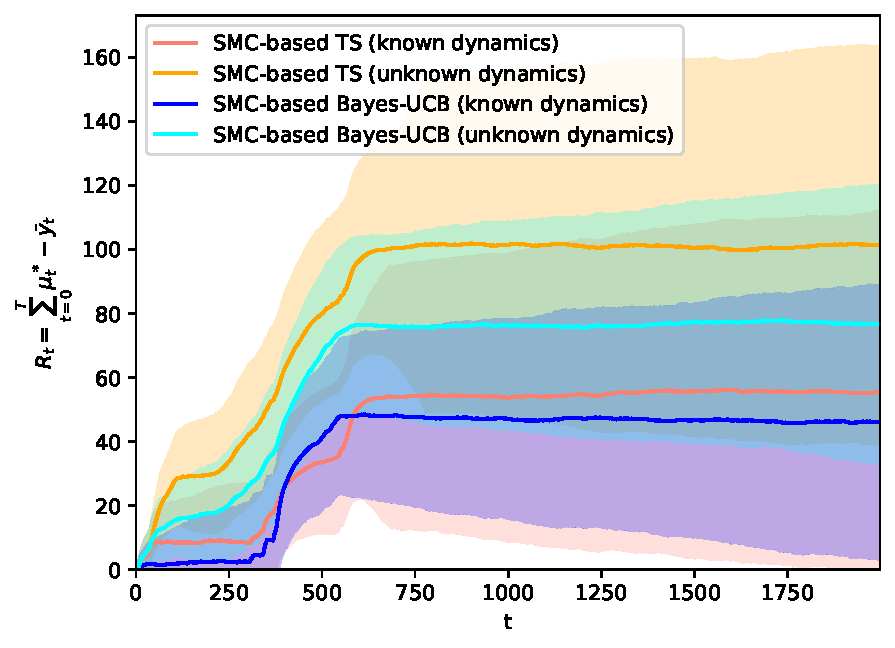
\includegraphics[width=\textwidth]{./fods_figs/dynamic/linearGaussian/a_M2000_cumulative_regret_dunknown}
		\caption{Cumulative regret for SMC-based Bayesian policies in scenario A: unknown dynamic parameters $L_a,\Sigma_a,\sigma_a^2, \forall a$.}
		\label{fig:dynamic_bandits_linearGaussian_a_cstatic_dunknown}
	\end{subfigure}\qquad
	\begin{subfigure}[b]{0.47\textwidth}
		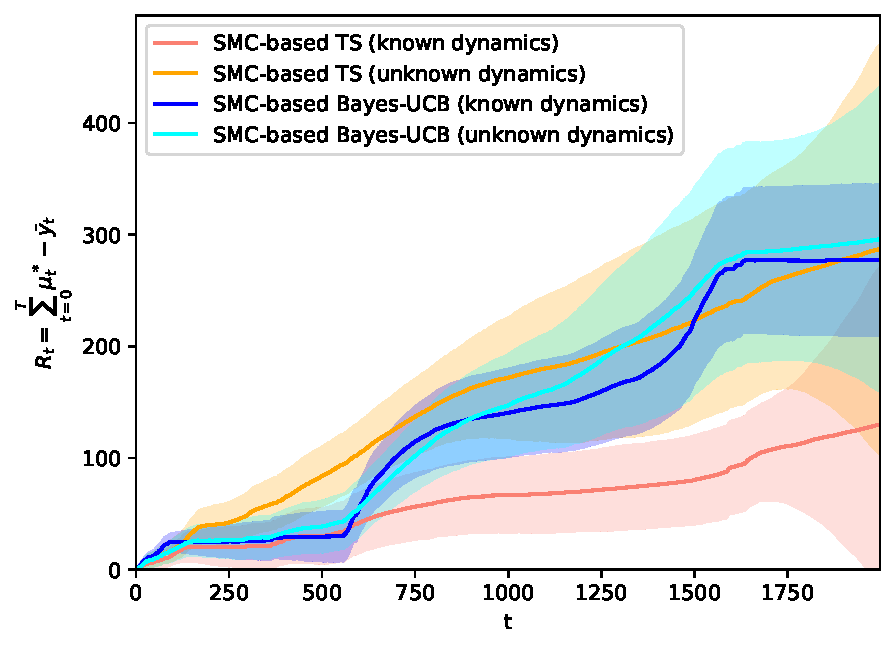
\includegraphics[width=\textwidth]{./fods_figs/dynamic/linearGaussian/b_M2000_cumulative_regret_dunknown}
		\caption{Cumulative regret for SMC-based Bayesian policies in scenario B: unknown dynamic parameters $L_a,\Sigma_a,\sigma_a^2, \forall a$.}
		\label{fig:dynamic_bandits_linearGaussian_b_cstatic_dunknown}
	\end{subfigure}
	\caption{
		Mean regret (standard deviation shown as shaded region) in contextual, linear Gaussian bandit Scenarios A and B
		described in Equations~\eqref{eq:linear_mixing_dynamics_a}--\eqref{eq:linear_mixing_dynamics_b},
		in the realistic setting of unknown dynamic parameters.
		Notice how
			in Figures~\ref{fig:dynamic_bandits_linearGaussian_a_cstatic_dknown_unknownsigma}--\ref{fig:dynamic_bandits_linearGaussian_b_cstatic_dunknown}
		the regret increases when the optimal arms swap
			(as shown in Figures~\ref{fig:linear_mixing_dynamics_a_gaussian_2}--\ref{fig:linear_mixing_dynamics_b_gaussian_2}).
		SMC-based policies find the right exploration-exploitation tradeoff even when the latent dynamic parameters are unknown.}
	\label{fig:dynamic_bandits_linearGaussian_dunknown}
\end{figure}


\clearpage
\subsection{Non-stationary, logistic rewards}
\label{ssec:dynamic_bandits_logistic}
% !TEX root = smc_bandits.tex
We here evaluate non-stationary, contextual, binary reward bandits.
We resort to the logistic reward function described in Equation~\eqref{eq:logistic_rewards},
with time-varying, latent parameter dynamics as described in the following scenarios:
\begin{equation}
\text{Scenario C}
\begin{cases}
\vspace*{1ex}
p(\theta_{t,a=0}|\theta_{t-1,a=0}): \\ \vspace*{1ex}
\hspace*{10ex}\begin{pmatrix}
\theta_{t,a=0,0}\\
\theta_{t,a=0,1}\\
\end{pmatrix} = \begin{pmatrix}
0.9 & -0.1 \\
-0.1 & 0.9 \\
\end{pmatrix} \begin{pmatrix}
\theta_{t-1,a=0,0}\\
\theta_{t-1,a=0,1}\\
\end{pmatrix} + \epsilon_{a=0} \;, \\ \vspace*{1ex}
\hspace*{40ex} \text{where } \;  \epsilon_{a=0} \sim \N{\epsilon|0,0.01 \cdot\mathrm{I}},\\

\vspace*{1ex}
p(\theta_{t,a=1}|\theta_{t-1,a=1}): \\ \vspace*{1ex}
\hspace*{10ex}\begin{pmatrix}
\theta_{t,a=1,0}\\
\theta_{t,a=1,1}\\
\end{pmatrix} = \begin{pmatrix}
0.9 & 0.1 \\
0.1 & 0.9 \\
\end{pmatrix} \begin{pmatrix}
\theta_{t-1,a=1,0}\\
\theta_{t-1,a=1,1}\\
\end{pmatrix} + \epsilon_{a=1}  \;, \\ \vspace*{1ex}
\hspace*{40ex} \text{where } \;  \epsilon_{a=1} \sim \N{\epsilon|0,0.01 \cdot\mathrm{I}},\\

p_a(Y|x,\theta_{t,a})=\frac{e^{y\cdot(x^\top\theta_{t,a}) }}{1+e^{(x^\top\theta_{t,a})}} \; .
\end{cases}
\label{eq:linear_mixing_dynamics_c}
\end{equation}

\begin{equation}
\text{Scenario D}
\begin{cases}
\vspace*{1ex}
p(\theta_{t,a=0}|\theta_{t-1,a=0}): \\ \vspace*{1ex}
\hspace*{10ex}\begin{pmatrix}
\theta_{t,a=0,0}\\
\theta_{t,a=0,1}\\
\end{pmatrix} = \begin{pmatrix}
0.5 & 0.0 \\
0.0 & 0.5 \\
\end{pmatrix} \begin{pmatrix}
\theta_{t-1,a=0,0}\\
\theta_{t-1,a=0,1}\\
\end{pmatrix} + \epsilon_{a=0}  \;, \\ \vspace*{1ex}
\hspace*{40ex} \text{where } \;  \epsilon_{a=0} \sim \N{\epsilon|0,0.01 \cdot\mathrm{I}},\\

\vspace*{1ex}
p(\theta_{t,a=1}|\theta_{t-1,a=1}): \\ \vspace*{1ex}
\hspace*{10ex}\begin{pmatrix}
\theta_{t,a=1,0}\\
\theta_{t,a=1,1}\\
\end{pmatrix} = \begin{pmatrix}
0.9 & 0.1 \\
0.1 & 0.9 \\
\end{pmatrix} \begin{pmatrix}
\theta_{t-1,a=1,0}\\
\theta_{t-1,a=1,1}\\
\end{pmatrix} + \epsilon_{a=1}  \;, \\ \vspace*{1ex}
\hspace*{40ex} \text{where } \;  \epsilon_{a=1} \sim \N{\epsilon|0,0.01 \cdot\mathrm{I}}, \\

p_a(Y|x,\theta_{t,a})=\frac{e^{y\cdot(x^\top\theta_{t,a}) }}{1+e^{(x^\top\theta_{t,a})}} \; .
\end{cases}
\label{eq:linear_mixing_dynamics_d}
\end{equation}

For bandits with logistic rewards,
there are no closed form posteriors;
hence, one needs to resort to approximations,
\eg a Laplace approximation as in~\citep{ic-Chapelle2011} for the stationary case.
However, there are no bandit algorithms for the non-stationary logistic scenarios described above.
%
On the contrary, SMC-based Bayesian policies can easily accommodate this setting,
by updating posterior random measures $p_M(\theta_{t}|\HH_{1:t})$ as in Algorithm~\ref{alg:sir-mab},
for both stationary (evaluated in Appendix~\ref{assec:static_bandits_experiments_logistic}) and non-stationary bandits we report here.

Figure~\ref{fig:dynamic_bandits_logistic} illustrates how
SMC-based Bayesian policies adapt to non-stationary optimal arm switches under contextual, binary reward observations,
achieving sublinear regret.
Results in Figures~\ref{fig:linear_mixing_dynamics_d_logistic}--\ref{fig:dynamic_bandits_d_logistic_cstatic}
also showcase how a bandit agent's regret suffers when learning unknown parameters of the latent dynamics.
%
Even though this is a particularly challenging problem,
presented evidence suggests that
SMC-based policies do learn the underlying latent dynamics from contextual binary rewards.

Notably, proposed policies are able to successfully identify which arm to play:
\ie both \textit{SMC-based TS and SMC-based UCB} ---with no dynamic parameter knowledge---
are able to flatten their regret
for $t\geq 650$ in Figure~\ref{fig:dynamic_bandits_c_logistic_cstatic} and
$t\geq 1750$ in Figure~\ref{fig:dynamic_bandits_d_logistic_cstatic}.

% Logistic results 
\begin{figure}[!h]
	\begin{subfigure}[b]{0.45\textwidth}
		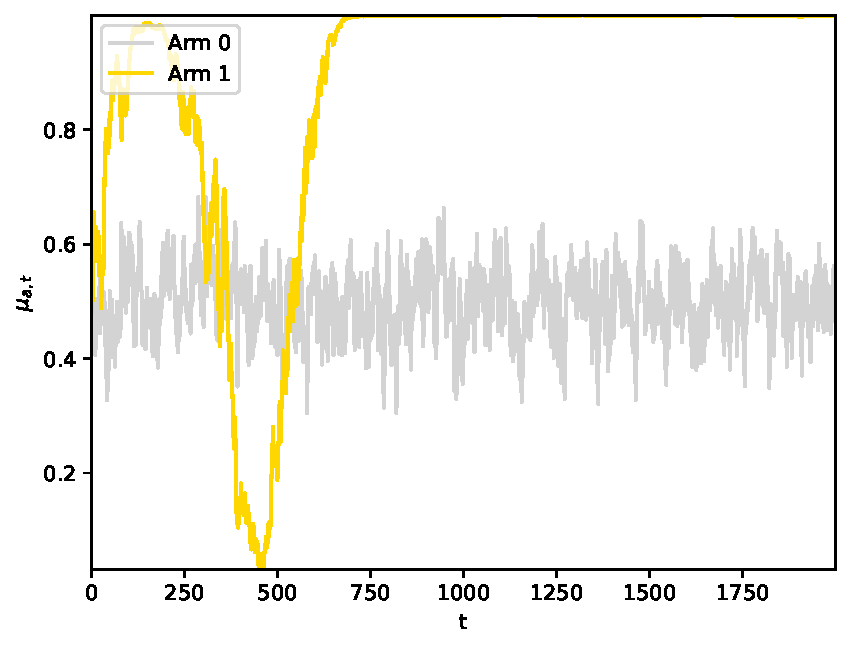
\includegraphics[width=\textwidth]{./fods_figs/dynamic/logistic/dynamics_c}
		\caption{Expected per-arm rewards over time for Scenario C in Equation~\eqref{eq:linear_mixing_dynamics_c}.
			Notice the early optimal arm change at $t\approx600$.
		}
		\label{fig:linear_mixing_dynamics_c_logistic}
	\end{subfigure}\qquad
	\begin{subfigure}[b]{0.45\textwidth}
		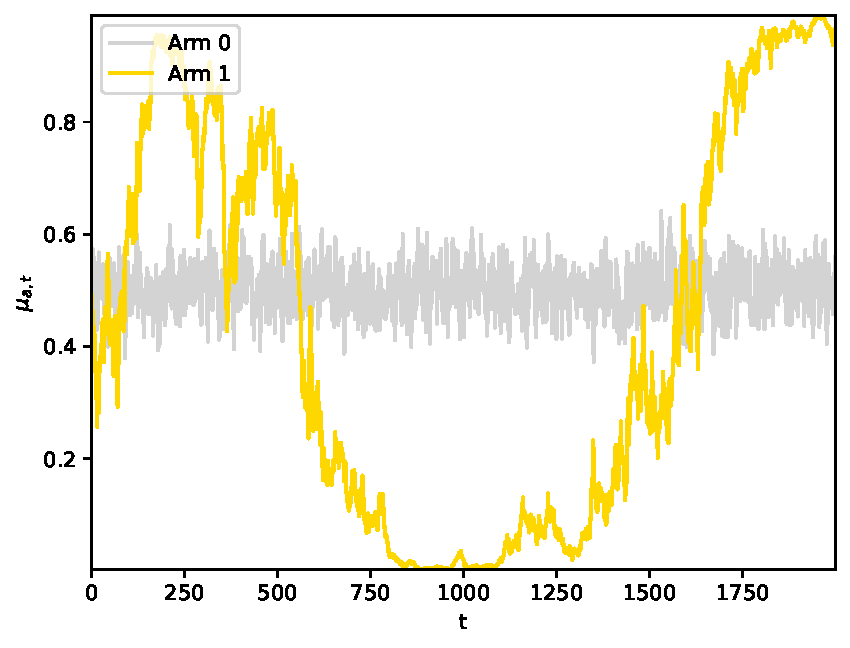
\includegraphics[width=\textwidth]{./fods_figs/dynamic/logistic/dynamics_d}
		\caption{Expected per-arm rewards over time for Scenario D in Equation~\eqref{eq:linear_mixing_dynamics_d}.
			Notice the late optimal arm change at $t\approx1650$.
		}
		\label{fig:linear_mixing_dynamics_d_logistic}
	\end{subfigure}
	
	\begin{subfigure}[b]{0.47\textwidth}
		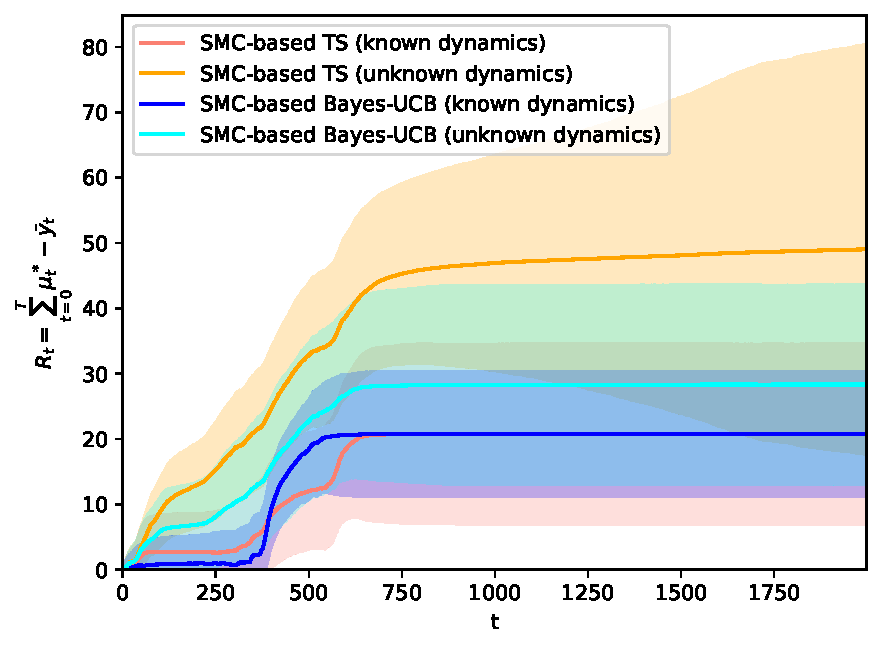
\includegraphics[width=\textwidth]{./fods_figs/dynamic/logistic/c_M2000_cumulative_regret_dunknown}
		\caption{Cumulative regret for SMC-based Bayesian policies in scenario C: known and unknown dynamic parameters.}
		\label{fig:dynamic_bandits_c_logistic_cstatic}
	\end{subfigure}\qquad
	\begin{subfigure}[b]{0.47\textwidth}
		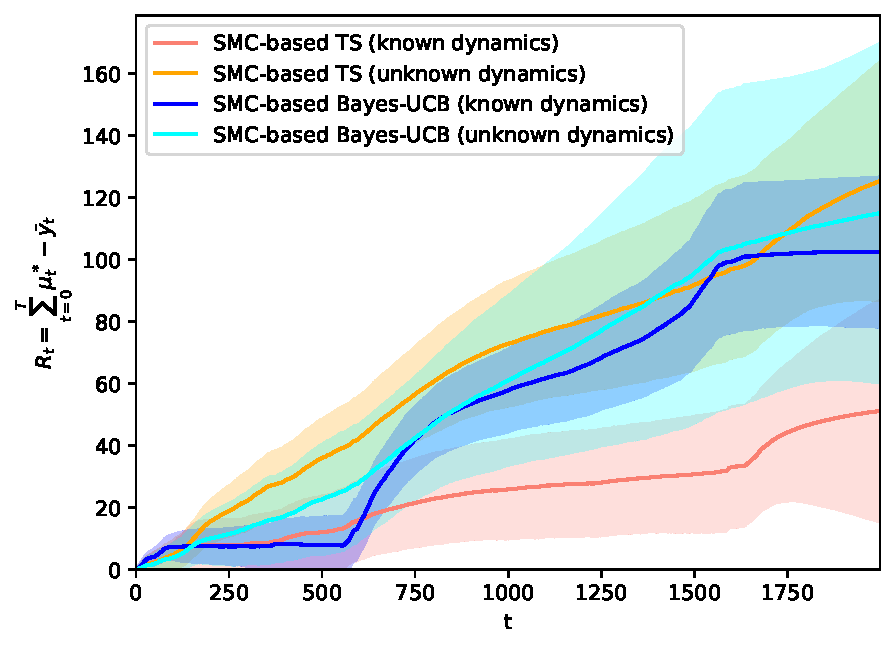
\includegraphics[width=\textwidth]{./fods_figs/dynamic/logistic/d_M2000_cumulative_regret_dunknown}
		\caption{Cumulative regret for SMC-based Bayesian policies in scenario D: known and unknown dynamic parameters.}
		\label{fig:dynamic_bandits_d_logistic_cstatic}
	\end{subfigure}
	\caption{
		Mean regret (standard deviation shown as shaded region) in contextual linear logistic dynamic bandit Scenarios C and D
		described in Equations~\eqref{eq:linear_mixing_dynamics_c}--\eqref{eq:linear_mixing_dynamics_d}.
		Notice the difference in early ($t\approx600$ in Scenario C) and late ($t\approx1650$ in Scenario D) optimal arm changes,
			as illustrated in Figures~\ref{fig:linear_mixing_dynamics_c_logistic}--\ref{fig:linear_mixing_dynamics_d_logistic},
		and their impact in regret,
			as showcased in Figures~\ref{fig:dynamic_bandits_c_logistic_cstatic}--\ref{fig:dynamic_bandits_d_logistic_cstatic}.
		SMC-based Bayesian policies adapt and find the right exploration-exploitation tradeoff.}
	\label{fig:dynamic_bandits_logistic}
\end{figure}


\clearpage
\subsection{Non-stationary, categorical rewards}
\label{ssec:dynamic_bandits_categorical}
% !TEX root = smc_bandits.tex
We evaluate SMC-based Bayesian policies in a bandit setting that remains elusive to state-of-the-art bandit algorithms:
non-stationary bandits with discrete-categorical, contextual rewards.
%
We simulate the following two- and three-armed categorical bandit scenarios,
where numerical rewards $Y=c$, for $c\in\{0,1,2\}$,
depend on a two-dimensional context $x_t\in\Real^2$,
with time-varying parameters $\theta_{a,c,t}$
obeying the following dynamics:

\begin{equation}
\text{Scenario E}
\begin{cases}
\vspace*{1ex}
p(\theta_{t,a=0,c}|\theta_{t-1,a=0,c})\;, \; \forall c \in \{0,1,2\}:\\ \vspace*{1ex}
\hspace*{10ex}\begin{pmatrix}
\theta_{t,a=0,c,0}\\
\theta_{t,a=0,c,1}\\
\end{pmatrix} = \begin{pmatrix}
0.9 & -0.1 \\
-0.1 & 0.9 \\
\end{pmatrix} \begin{pmatrix}
\theta_{t-1,a=0,c,0}\\
\theta_{t-1,a=0,c,1}\\
\end{pmatrix} + \epsilon_{a=0,c} \;, \\ \vspace*{1ex}
\hspace*{38ex} \text{where } \; \epsilon_{a=0,c} \sim \N{\epsilon|0,0.01 \cdot\mathrm{I}}, \\

\vspace*{1ex}
p(\theta_{t,a=1,c}|\theta_{t-1,a=1,c})\;, \; \forall c \in \{0,1,2\}:\\ \vspace*{1ex}
\hspace*{10ex}\begin{pmatrix}
\theta_{t,a=1,c,0}\\
\theta_{t,a=1,c,1}\\
\end{pmatrix} = \begin{pmatrix}
0.9 & 0.1 \\
0.1 & 0.9 \\
\end{pmatrix} \begin{pmatrix}
\theta_{t-1,a=1,c,0}\\
\theta_{t-1,a=1,c,1}\\
\end{pmatrix} + \epsilon_{a=1,c} \;, \\ \vspace*{1ex}
\hspace*{38ex} \text{where } \;  \epsilon_{a=1,c} \sim \N{\epsilon|0,0.01 \cdot\mathrm{I}},\\

p_a(Y=c|x,\theta_{t,a})=\frac{e^{(x^\top\theta_{t,a,c})}}{\sum_{c'=1}^C e^{(x^\top\theta_{t,a,c'})} } \; .
\end{cases}
\label{eq:linear_mixing_dynamics_e}
\end{equation}

\begin{equation}
\text{Scenario F}
\begin{cases}
\vspace*{1ex}
p(\theta_{t,a=0,c}|\theta_{t-1,a=0,c}) \;, \; \forall c \in \{0,1,2\}:\\ \vspace*{1ex}
\hspace*{10ex}\begin{pmatrix}
\theta_{t,a=0,c,0}\\
\theta_{t,a=0,c,1}\\
\end{pmatrix} = \begin{pmatrix}
0.9 & -0.1 \\
-0.1 & 0.9 \\
\end{pmatrix} \begin{pmatrix}
\theta_{t-1,a=0,c,0}\\
\theta_{t-1,a=0,c,1}\\
\end{pmatrix} + \epsilon_{a=0,c} \;, \\ \vspace*{1ex}
\hspace*{38ex} \text{where } \; \epsilon_{a=0,c} \sim \N{\epsilon|0,0.01 \cdot\mathrm{I}}, \\

\vspace*{1ex}
p(\theta_{t,a=1,c}|\theta_{t-1,a=1,c})\;, \; \forall c \in \{0,1,2\}:\\ \vspace*{1ex}
\hspace*{10ex}\begin{pmatrix}
\theta_{t,a=1,c,0}\\
\theta_{t,a=1,c,1}\\
\end{pmatrix} = \begin{pmatrix}
0.9 & 0.1 \\
0.1 & 0.9 \\
\end{pmatrix} \begin{pmatrix}
\theta_{t-1,a=1,c,0}\\
\theta_{t-1,a=1,c,1}\\
\end{pmatrix} + \epsilon_{a=1,c} \;, \\ \vspace*{1ex}
\hspace*{38ex} \text{where } \; \epsilon_{a=1,c} \sim \N{\epsilon|0,0.01 \cdot\mathrm{I}},\\

\vspace*{1ex}
p(\theta_{t,a=2,c}|\theta_{t-1,a=2,c})\;, \; \forall c \in \{0,1,2\}:\\ \vspace*{1ex}
\hspace*{10ex}\begin{pmatrix}
\theta_{t,a=2,c,0}\\
\theta_{t,a=2,c,1}\\
\end{pmatrix} = \begin{pmatrix}
0.9 & 0.1 \\
0.1 & 0.9 \\
\end{pmatrix} \begin{pmatrix}
\theta_{t-1,a=2,c,0}\\
\theta_{t-1,a=2,c,1}\\
\end{pmatrix} + \epsilon_{a=2,c} \;, \\ \vspace*{1ex}
\hspace*{38ex} \text{where } \; \epsilon_{a=2,c} \sim \N{\epsilon|0,0.01 \cdot\mathrm{I}},\\

p_a(Y=c|x,\theta_{t,a})=\frac{e^{(x^\top\theta_{t,a,c})}}{\sum_{c'=1}^C e^{(x^\top\theta_{t,a,c'})} } \; .
\end{cases}
\label{eq:linear_mixing_dynamics_f}
\end{equation}

These bandit scenarios accommodate a diverse set of expected reward dynamics,
for each realization of the noise processes $\epsilon_{a,c}, \forall a,c$,
and depending on the initialization of parameters $\theta_{0,a}$.
%
We illustrate per-arm, expected reward time-evolution for a realization
of the two-armed bandit Scenario E in Figure~\ref{fig:linear_mixing_dynamics_e_softmax},
and for the three-armed bandit Scenario F in Figure~\ref{fig:linear_mixing_dynamics_f_softmax}.

In all cases, expected rewards of each arm vary over time,
resulting in transient and recurrent swaps of the optimal arm's identity.
We show the corresponding cumulative regret of SMC-based Bayesian policies
in Figure~\ref{fig:dynamic_bandits_e_softmax_cstatic} for Scenario E,
and in Figure~\ref{fig:dynamic_bandits_f_softmax_cstatic} for Scenario F.

\begin{figure}[!ht]
	\centering
	\begin{subfigure}[b]{0.47\textwidth}
		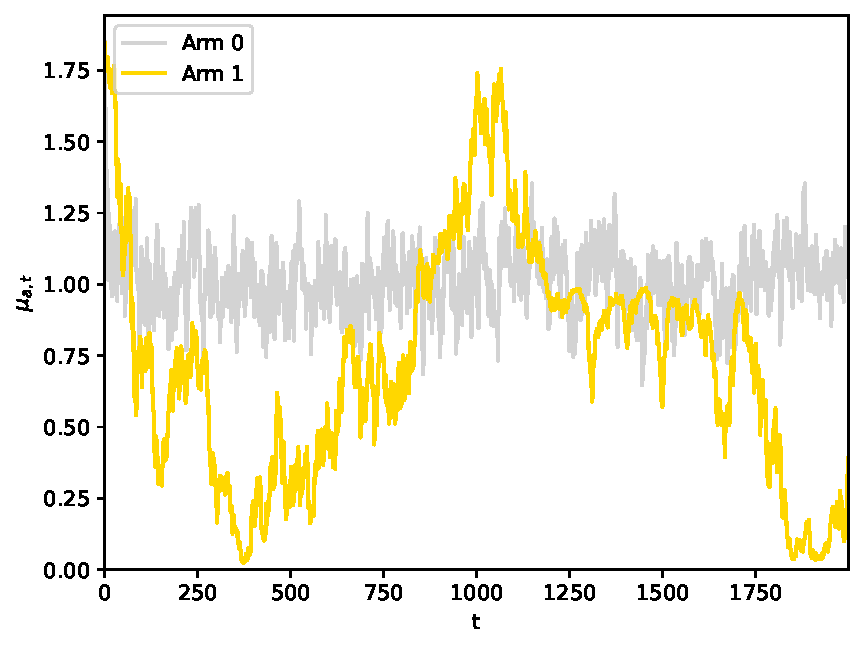
\includegraphics[width=\textwidth]{./fods_figs/dynamic/softmax/dynamics_e}
		\caption{Expected per-arm rewards over time for Scenario E in Equation~\eqref{eq:linear_mixing_dynamics_e}.
			Notice the optimal arm changes around $t\approx1000$.}
		\label{fig:linear_mixing_dynamics_e_softmax}%
	\end{subfigure}\qquad
	\begin{subfigure}[b]{0.47\textwidth}
		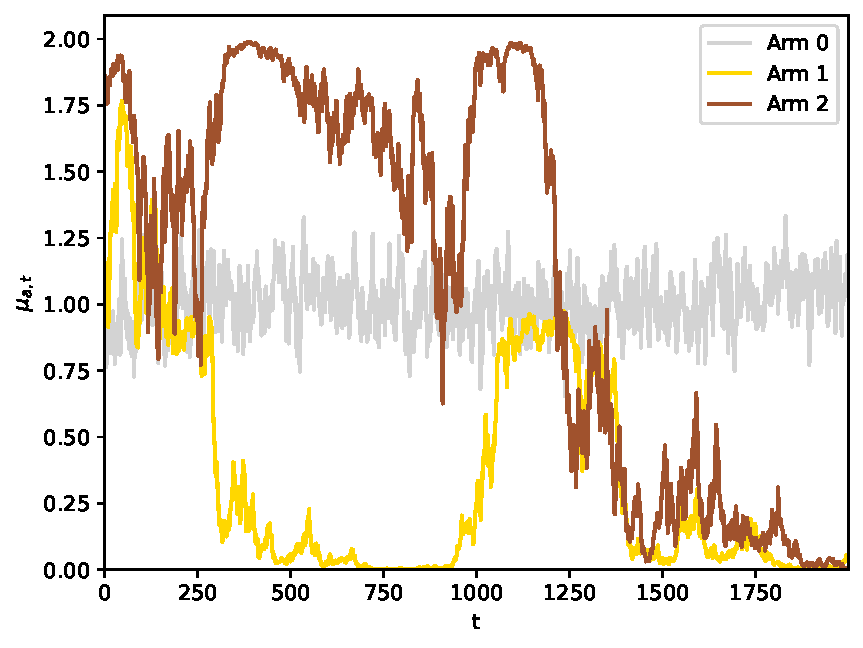
\includegraphics[width=\textwidth]{./fods_figs/dynamic/softmax/dynamics_f}
		\caption{Expected per-arm rewards over time for Scenario F in Equation~\eqref{eq:linear_mixing_dynamics_e}.
			Notice the optimal arm change around $t\approx1250$.}
		\label{fig:linear_mixing_dynamics_f_softmax}
	\end{subfigure} %
	
	\begin{subfigure}[b]{0.47\textwidth}
		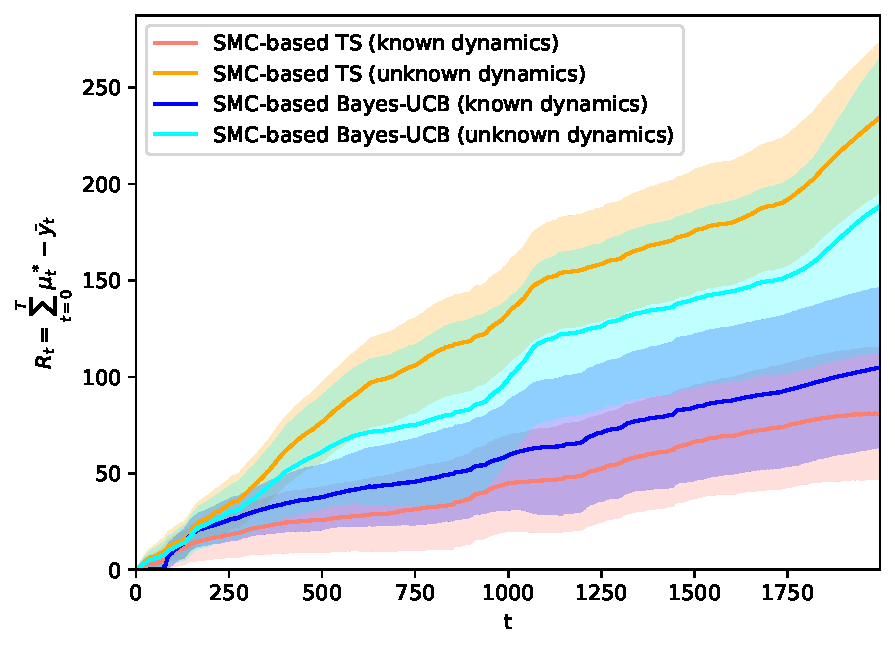
\includegraphics[width=\textwidth]{./fods_figs/dynamic/softmax/e_M2000_cumulative_regret_dunknown}
		\caption{Cumulative regret for SMC-based Bayesian policies in scenario E: known and unknown dynamic parameters.}
		\label{fig:dynamic_bandits_e_softmax_cstatic}%
	\end{subfigure}\qquad
	\begin{subfigure}[b]{0.47\textwidth}
		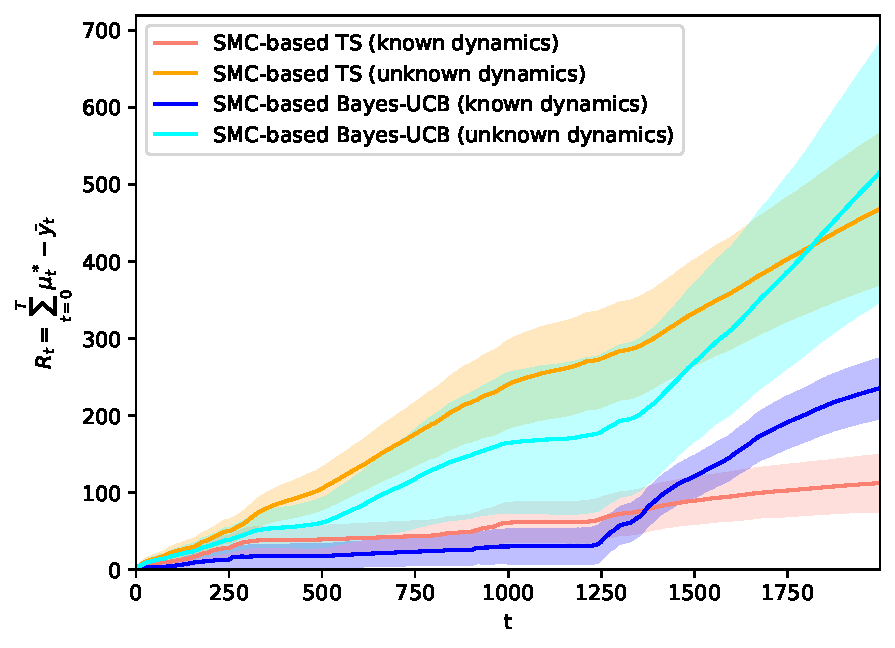
\includegraphics[width=\textwidth]{./fods_figs/dynamic/softmax/f_M2000_cumulative_regret_dunknown}
		\caption{Cumulative regret for SMC-based Bayesian policies in scenario F: known and unknown dynamic parameters.}
		\label{fig:dynamic_bandits_f_softmax_cstatic}%
	\end{subfigure}
	
	\caption{
		%Per-arm, expected reward evolution over time of two-armed contextual non-stationary categorical bandit Scenarios E and F
		%	described in Equations~\eqref{eq:linear_mixing_dynamics_e}--\eqref{eq:linear_mixing_dynamics_f}
		%	in Figures~\ref{fig:linear_mixing_dynamics_e_softmax}--\ref{fig:linear_mixing_dynamics_f_softmax}.
		Mean regret (standard deviation shown as shaded region) in contextual, non-stationary categorical bandit Scenarios E and F
		described in Equations~\eqref{eq:linear_mixing_dynamics_e}--\eqref{eq:linear_mixing_dynamics_f}.
		Notice how changes in per-arm expected rewards ($t\approx1750$ in Scenario E and $t>1250$ in Scenario F) 
		as illustrated in Figures~\ref{fig:linear_mixing_dynamics_e_softmax}--\ref{fig:linear_mixing_dynamics_f_softmax}
		impact regret
		as showcased in Figures~\ref{fig:dynamic_bandits_e_softmax_cstatic}--\ref{fig:dynamic_bandits_f_softmax_cstatic}.
		SMC-based Bayesian policies adapt to these changes and balance the exploration-exploitation tradeoff.
	}
	\label{fig:dynamic_bandits_softmax}
\vspace*{-2ex}
\end{figure}

We observe that SMC-based Thompson sampling and Bayes-UCB are able to reach
satisfactory exploitation-exploration balance,
\ie the algorithms dynamically adapt their choice of which arm to play, and attain sublinear cumulative regret.

Recall the linear increase in cumulative regret (\ie exploration)
when latent parameter dynamics result in changes in the optimal arm's identity:
around $t\in (800,1000)$ in Figure~\ref{fig:dynamic_bandits_e_softmax_cstatic},
and around $t\in (1250,1500)$ in Figure~\ref{fig:dynamic_bandits_f_softmax_cstatic}.
%
After updating the random measure posterior over the unknown latent parameters,
and recomputing the expected rewards per-arm,
SMC-based policies are able to slowly adapt to the optimal arm changes,
reaching a new exploitation-exploration balance, \ie flattening the cumulative regret curves.

For the most interesting and challenging setting where the dynamic model's parameters are unknown,
we observe an increase in cumulative regret for both SMC-based policies.
This is a direct consequence of
the agent sequentially learning all the unknown model parameters,
per-arm $a$, and discrete value $c$: $L_{a,c}, \Sigma_{a,c}, \forall a,c$.
%
Only when posteriors over these 
---used by the SMC-based agents to propagate uncertainty to each bandit arms' expected reward estimates---
are improved,
can SMC-based policies make informed decisions and attain sublinear regret.

We observe that the impact of expected reward changes,
when occurring later in time
(\eg $t\approx1250$ in Figure~\ref{fig:linear_mixing_dynamics_f_softmax})
is more pronounced for SMC-based Bayes-UCB policies.
Namely, the average cumulative regret of SMC-based Bayes-UCB increases drastically, as well as its volatility,
after $t=1250$ in Figure~\ref{fig:dynamic_bandits_f_softmax_cstatic}.
%
We hypothesize that this deterioration over time is
due to the shrinking quantile value $\alpha_t\propto1/t$ proposed by \citet{ip-Kaufmann2012}, 
originally designed for stationary bandits.
Confidence bounds for static reward models tend to shrink proportional to the number of observations per bandit arm.
However, in non-stationary regimes, such assumption does not hold:
shrinking $\alpha_t$ over time does not capture the time-evolving parameter posteriors' uncertainty in the long run. 

More generally, the need to determine appropriate quantile values $\alpha_t$
for each reward and non-stationary bandit model is a drawback of Bayes-UCB,
as its optimal value will depend on the specific combination of underlying dynamics and reward function.
%
On the contrary, Thompson sampling relies on samples from the posterior,
which we here show SMC is able to approximate accurately enough
for SMC-based Thompson sampling to operate successfully in all studied cases,
without any hyperparameter selection.




%\clearpage
\subsection{Bandits for personalized news article recommendation}
\label{ssec:logged_data_bandits}
% !TEX root = smc_bandits.tex
We evaluate the application of SMC-based policies in a real-life application of bandits:
the recommendation of personalized news articles, as previously done by \citet{ic-Chapelle2011}.
%Online content recommendation represents an important example of reinforcement learning, as it requires efficient balancing of the exploration and exploitation tradeoff.
%

We use a dataset\footnote{
	Available at \href{https://webscope.sandbox.yahoo.com/catalog.php?datatype=r\&did=49}{R6A - Yahoo! Front Page Today Module User Click Log Dataset.}
} that contains a fraction of user click logs for news articles displayed in the Featured Tab of the Today Module on the Yahoo! Front Page during the first ten days in May 2009. The articles to be displayed were originally chosen uniformly at random from a hand-picked pool of high-quality articles.
From these pool of original candidates,
we pick a subset of 20 articles shown at different times within May 6th,
and collect all user interactions logged with these articles,
for a total of 500,354 events.
In the dataset,
each user is associated with six features:
a bias term and 5 features that correspond to the membership features constructed via the conjoint analysis with a bilinear model described in~\citep{ip-Chu2009}.

The goal is to identify the most interesting article for each user,
or in bandit terms,
to maximize the total number of clicks on the recommended articles over all user interactions,
\ie the average click-through rate (CTR).

We treat each article as a bandit arm ($|\A|=20$),
and define whether the article is clicked or not by the user as a binary reward: $y_t=\{1,0\}$.
Hence, we pose the problem as a MAB with logistic rewards,
where we incorporate the user features as context, $x_t\in \Real^6$.

We implement SMC-based Thompson sampling only, due to the flexibility shown in simulated scenarios,
and its lack of hyperparameter tuning.

We argue that a news recommendation system should evolve over time,
as the relevance of news might change during the course of the day.
We evaluate both stationary and non-stationary bandits with logistic rewards.

As shown in Figure~\ref{fig:yahoo_logistic_dynamic},
we observe the flexibility of a non-stationary logistic bandit model,
where we notice how the SMC-based TS agent is able to pick up the dynamic popularity of certain articles over time
---averaged CTR results are provided in Table \ref{tab:yahoo_logistic_crt}.

% Figure
\begin{figure}[!h]
	\centering
	\vspace*{-2ex}
	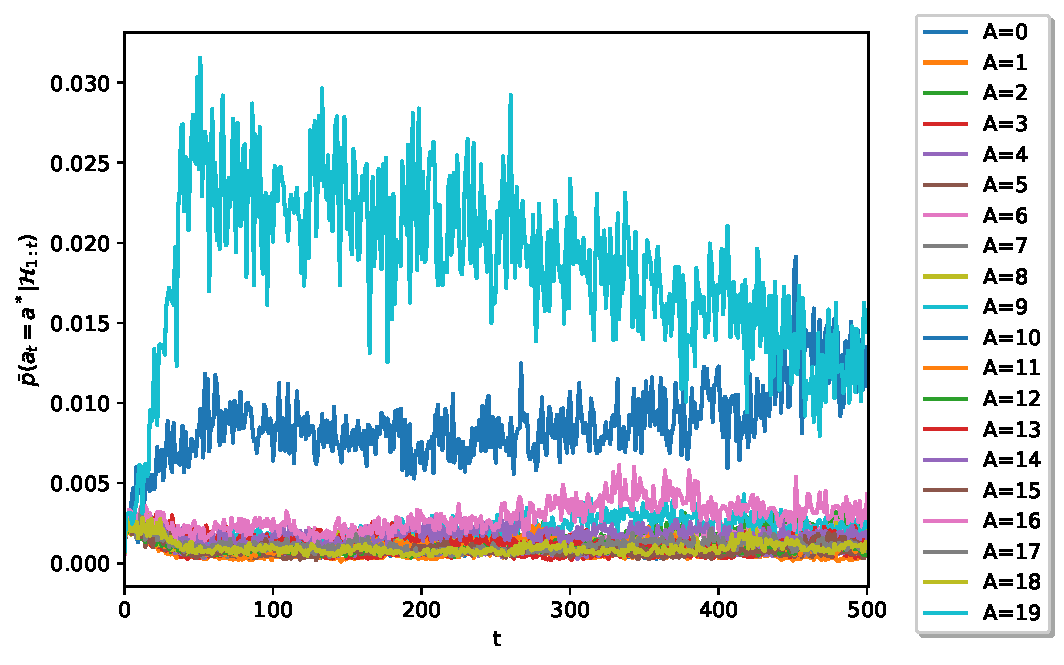
\includegraphics[width=0.85\textwidth]{./fods_figs/yahoo/yahoo_logistic_dynamic}
	\vspace*{-2ex}
	\caption{Empirical probability of playing each bandit arm over time, for SMC-based dynamic logistic Thompson sampling.
		The proposed dynamic bandit policy captures the changing popularity of articles over time.}
	\label{fig:yahoo_logistic_dynamic}
\end{figure}

% Table
%%%%%%%%%%%%%%%%%%%%%%%%
%% Table for yahoo data with logistic bandits
%%%%%%%%%%%%%%%%%%%%%%%%
\begin{table}[!ht]
	\begin{center}
		\resizebox*{\textwidth}{!}{
			\begin{tabular}{*{3}{|c}|}
				\hline
				% Header
				Model \cellcolor[gray]{0.6} & CTR\cellcolor[gray]{0.6} & Normalized CTR\cellcolor[gray]{0.6} \\ \hline
				% table starts
				\cellcolor[gray]{0.8} Logistic rewards, static arms & 0.0670 +/- 0.0088 & 1.6095 +/- 0.2115  \\ \hline
				\cellcolor[gray]{0.8} Logistic rewards, time-evolving arms & 0.0655 +/- 0.0082 & 1.5745 +/- 0.2064 \\ \hline
			\end{tabular}
		}
		\caption{CTR results for SMC-based policies on the news article recommendation dataset.
			The normalized CTR is with respect to a random recommendation baseline.}
		\label{tab:yahoo_logistic_crt}
	\end{center}
	\vspace*{-2ex}
\end{table}



\section{Conclusion}
\label{sec:conclusion}

We contribute to the field of sequential decision processes by proposing a Bayesian nonparametric mixture model based Thompson sampling.
We merge advances in the field of Bayesian nonparametrics with a state-of-the art MAB policy (\ie Thompson sampling), allowing for its extension to complex multi-armed bandit domains where there is model uncertainty.

The proposed algorithm provides flexible modeling of convoluted reward functions with convergence guarantees, and attains the exploration-exploitation trade-off in complex MABs with minimal assumptions.

We provide an asymptotic upper bound for the expected cumulative regret of the proposed Dirichlet process Gaussian mixture model based Thompson sampling.

In addition, empirical results show improved cumulative regret performance of the proposed nonparametric Thompson sampling in challenging domains ---where there is model uncertainty--- remarkably adjusting to the complexity of the underlying bandit in an online fashion ---bypassing model mispecification and hyperparameter tuning.

Important savings are attained for complex bandit settings (\eg unbalanced and heavy tailed reward distributions, and bandits with different per-arm reward distributions), where alternative methods struggle.

The competitive advantage lies on the capacity of Bayesian nonparametrics to adjust the complexity of the posterior density to the sequentially observed bandit data.
With the ability to sequentially learn the Bayesian nonparametric mixture model that best approximates the true reward distribution ---not necessarily in the exponential family--- the proposed method can be applied to diverse MAB settings without stringent model specifications and attain reduced regret.

A future direction is to tighten the presented regret bound, as well as to apply the proposed method to real-life MAB applications where complex models are likely to outperform simpler ones.

% BibTeX users please use one of
%\bibliography{../literature}   % name your BibTeX data base
% Select a .bst file for the style
\bibliographystyle{abbrvnat}
% For submission, need to paste the .bbl content here
\documentclass{article}
\usepackage[margin=1.5in]{geometry}

% insert here the call for the packages your document requires
%\usepackage{latexsym}
% Formatting
\usepackage{hyperref}       % hyperlinks
\usepackage{url}            % simple URL typesetting
\usepackage{enumitem}
\usepackage{ifthen}
\usepackage{sidecap}
\usepackage{helvet}
\usepackage{afterpage}
% Package added for words that contain a dash use \-/
\usepackage[shortcuts]{extdash}
\usepackage[htt]{hyphenat}
% Math
\usepackage{amsmath}
\usepackage{amsfonts}	% blackboard math symbols
\usepackage{mathtools}	% For \coloneq
\usepackage{nicefrac}       % compact symbols for 1/2, etc.
\usepackage{microtype}      % microtypography
\usepackage{dsfont} % Indicator that works with Type1

% Graphics
\usepackage{graphicx}
\usepackage{caption}
\usepackage{subcaption}
\usepackage{wrapfig}
\usepackage{float} %Stay where told

% Tables
\usepackage{booktabs}       % professional-quality tables
\usepackage{multirow} % to be able to have multiple row expanding cell
\usepackage[table]{xcolor}
\usepackage{arydshln} % For hdashline% New column types, left/center/right text aligned, given horizontal width
\usepackage{ragged2e} % To justify table text
\newcolumntype{L}[1]{>{\raggedright\let\newline\\\arraybackslash\hspace{0pt}}m{#1}}
\newcolumntype{C}[1]{>{\centering\let\newline\\\arraybackslash\hspace{0pt}}m{#1}}
% For some reason, justify seems to add some vertical space, remove with vspace
\newcolumntype{J}[1]{>{\vspace*{-2ex}\justify\let\newline\\\arraybackslash\hspace{0pt}}m{#1}}
\newcolumntype{R}[1]{>{\raggedleft\let\newline\\\arraybackslash\hspace{0pt}}m{#1}}

% Algorithms
\usepackage{algorithm}
\usepackage{algorithmic}
% Theorems/lemmas
\usepackage{amsthm}
\newtheorem{theorem}{Theorem}[section]
\newtheorem{corollary}{Corollary}[theorem]
\newtheorem{lemma}[theorem]{Lemma}

% To draw graphs (load after xcolor to avoid options clash)
\usepackage{tikz}
\usetikzlibrary{bayesnet} % Library for bayesian networks

% Bibliography
\usepackage{natbib}
% To be able to have references in 2 columns with equal length
\usepackage{flushend}
% etc.
%
% please place your own definitions here and don't use \def but \newcommand{}{}
%%%% iurteaga definitions and macros
% Dolor definitions
%\def\bluecolor#1{\textcolor[rgb]{0,0,1}{\bf #1}}
%\def\greencolor#1{\textcolor[rgb]{0,1,0}{\bf #1}}
%\def\redcolor#1{\textcolor[rgb]{1,0,0}{\bf #1}}

% TODO
\newcommand{\TODO}[1]{\textcolor{red}{TODO: #1}}

% Abbreviations
\newcommand{\iid}{i.i.d. }
\newcommand{\ie}{i.e., }
\newcommand{\Ie}{I.e., }
\newcommand{\eg}{e.g., }
\newcommand{\Eg}{E.g., }
\newcommand{\etAl}{et al.\xspace}

% Real line
\newcommand{\Real}{{\mathbb R}} 
% Natural numbers
\newcommand{\Natural}{{\mathbb N}} 

% Probability related
\newcommand{\Prob}[1]{\mathbb{P}\left( #1 \right)}
% with 2 arguments, for probability model in subscript
\newcommand{\myProb}[2]{\mathbb{P}_{#1}\left( #2 \right)}
%Expected value
\newcommand{\eValue}[2]{\mathbb{E}_{#1}\left\{ #2 \right\}}
\newcommand{\Var}[1]{\mathbb{V}\mathrm{ar} \left\{ #1 \right\}}
\newcommand{\indep}{{\;\bot\!\!\!\!\!\!\bot\;}}
% Kullback-Leibler
\newcommand{\KL}[2]{\mathrm{KL}\left( #1 \| #2\right)}
% Distributions
\newcommand{\N}[1]{\mathcal{N}\left( #1\right)}
\newcommand{\MN}[1]{\mathcal{MN}\left( #1\right)}
\newcommand{\T}[1]{\mathcal{T}\left( #1\right)}
\newcommand{\MT}[1]{\mathcal{MT}\left( #1\right)}
\newcommand{\Dir}[1]{\mathcal{Dir}\left( #1\right)}
\newcommand{\Mult}[1]{{\rm Mult}\left( #1\right)}
\newcommand{\Cat}[1]{{\rm Cat}\left( #1\right)}
\newcommand{\Bin}[1]{{\rm Bin}\left( #1\right)}
\newcommand{\IG}[1]{\mathcal{IG}\left( #1\right)}
\newcommand{\NIG}[1]{\mathcal{NIG}\left( #1\right)}
\newcommand{\NIX}[1]{\mathcal{NIX}\left( #1\right)}
\newcommand{\IW}[1]{\mathcal{IW}\left( #1\right)}
\newcommand{\NIW}[1]{\mathcal{NIW}\left( #1\right)}
\newcommand{\Beta}[1]{\mathcal{Beta}\left( #1\right)}
\newcommand{\Ber}[1]{{\rm Ber}\left( #1\right)}
\newcommand{\U}[1]{\mathcal{U}\left( #1\right)}

% My small matrix
\newcommand{\mySmallMatrix}[1]{\left(\begin{smallmatrix} #1 \end{smallmatrix}\right)}
%Determinant
\newcommand{\mydet}[1]{\left| #1 \right|}
\newcommand{\tr}[1]{\mathrm{tr}\left\{ #1 \right\}} % trace
\newcommand{\diag}{\mathrm{diag}}
% My indicator function
\newcommand{\myind}[1]{\mathds{1}\left[#1\right]}
% d in integral
\newcommand{\dd}[1]{\mathrm{d} #1}

% Useful in Bandits
\newcommand{\A}{\mathcal{A}}
\newcommand{\Astar}{A^*}
\newcommand{\astar}{a^*}
\newcommand{\pstar}{p^*}
\newcommand{\pistar}{\pi^*}
\newcommand{\Atilde}{\tilde{A}}
\newcommand{\atilde}{\tilde{a}}
\newcommand{\ptilde}{\tilde{p}}
\newcommand{\pitilde}{\tilde{\pi}}
\newcommand{\thetastar}{\theta^*}
\newcommand{\thetatilde}{\tilde{\theta}}
\newcommand{\Y}{\mathcal{Y}}
\newcommand{\HH}{\mathcal{H}}

\newcommand{\myPi}[2]{\pi_{#1}\left( #2 \right)}
%\newcommand{\myPistar}[1]{\pi_{p^*}^*\left( #1 \right)}
\newcommand{\myPistar}[1]{\pi_{p^*}\left( #1 \right)}
%\newcommand{\myPitilde}[1]{\tilde{\pi}_{\ptilde}\left( #1 \right)}
\newcommand{\myPitilde}[1]{\pi_{\ptilde}\left( #1 \right)}

%Others
\newcommand{\eqd}{\stackrel{d}{=}} % equal in distribution/law/measure
\newcommand{\deq}{:=} % Define equality
\newcommand{\abs}[1]{|{#1}|}
\newcommand{\argmax}{\mathop{\mathrm{argmax}}}
\newcommand{\argmin}{\mathop{\mathrm{argmin}}}
\newcommand{\eps}{\varepsilon}
%%%%%%%% end iurteaga %%%%%%%% 

%%%%%%%% end iurteaga %%%%%%%% 

\title{Nonparametric Gaussian Mixture Models \\ for the Multi-Armed Contextual Bandit}

\author{ I\~{n}igo Urteaga and Chris H.~Wiggins\\
	{\sf \{inigo.urteaga, chris.wiggins\}@columbia.edu} \\\\
	Department of	Applied Physics and Applied Mathematics\\
	Data Science Institute\\
	Columbia University\\
	New York City, NY 10027
}

\begin{document}
	
\maketitle

\begin{abstract}
We here adopt Bayesian nonparametric mixture models to extend multi-armed bandits in general, and Thompson sampling in particular, to scenarios where there is reward model uncertainty. In the stochastic multi-armed bandit, where an agent must learn a policy that maximizes long term payoff, the reward for the selected action is generated from an unknown distribution. Thompson sampling is a generative and interpretable multi-armed bandit algorithm that has been shown both to perform well in practice, and to enjoy optimality properties for certain reward functions. Nevertheless, Thompson sampling requires knowledge of the true reward model, for calculation of expected rewards and sampling from its parameter posterior. In this work, we extend Thompson sampling to complex scenarios where there is model uncertainty, by adopting a very flexible set of reward distributions: Bayesian nonparametric Gaussian mixture models. The generative process of Bayesian nonparametric mixtures naturally aligns with the Bayesian modeling of multi-armed bandits: the nonparametric model autonomously determines its complexity as new rewards are observed for the played arms. By characterizing each arm's reward distribution with independent nonparametric mixture models, the proposed method sequentially learns the model that best approximates the true underlying reward distribution, achieving successful performance in complex ---not in the exponential family--- bandits. Our contribution is valuable for practical scenarios, as it avoids stringent case-by-case model specifications and hyperparameter tuning, yet attains reduced regret in diverse bandit settings.
\end{abstract}

\section{Introduction}
\label{sec:intro}
% !TEX root = main.tex
Sequential decision making aims to optimize interactions with the world (exploit), while simultaneously learning how the world operates (explore). The origins of the study of the exploration-exploitation trade-off can be traced back to the beginning of the past century, with important contributions within the field of statistics by~\citet{j-Thompson1935} and later~\citet{j-Robbins1952}.
The multi-armed bandit (MAB) is a natural abstraction for a wide variety of real-world challenges that require learning while simultaneously maximizing rewards~\citep{b-Lattimore2020}. The name `bandit' finds its origin in the playing strategy one must devise when facing a row of slot machines~\citep{j-Lai1985}. The contextual MAB, where at each interaction with the world side information (known as `context') is available, is a natural extension of the bandit problem. Recently, a renaissance of the study of MAB algorithms has flourished~\citep{ip-Agrawal2012,ip-Maillard2011}, attracting interest from industry as well, due to its impact in digital advertising and products~\citep{ip-Li2010}. 

\citet{j-Thompson1933} sampling %, also known as posterior sampling~\cite{j-Russo2014}, 
provides an elegant approach that tackles the exploration-exploitation dilemma in MABs. It updates a posterior over expected rewards for each arm, and chooses actions based on the probability that they are optimal. It has been empirically and theoretically proven to perform competitively for MAB models within the exponential family~\citep{ip-Agrawal2013a,ip-Agrawal2013,ic-Korda2013}. Its applicability to the more general reinforcement learning setting of Markov decision processes~\citep{j-Burnetas1997} has recently tracked momentum as well~\citep{ip-Gopalan2015,ic-Ouyang2017}.

Thompson sampling, and the Bayesian approach to the MAB problem, facilitate not only generative and interpretable modeling, but sequential and batch processing as well.
A Thompson sampling policy requires access to posterior samples of the model.
Unfortunately, maintaining such posterior is intractable for distributions not in the exponential family~\citep{j-Russo2018}.
Therefore, developing practical MAB methods to balance exploration and exploitation in real-life domains that might not pertain to such reward family remains largely unsolved.

In an effort to extend Thompson sampling to more complex scenarios, researchers have considered other flexible reward functions and Bayesian inference.
Recent approaches have embraced Bayesian neural networks and approximate inference for Thompson sampling. Variational methods, stochastic mini-batches, and Monte Carlo techniques have been studied for uncertainty estimation of reward posteriors~\citep{ip-Blundell2015, ic-Kingma2015, ip-Lipton2018, ic-Osband2016, ip-Li2016}.

~\citet{ip-Riquelme2018} have benchmarked such techniques and reported that neural networks with approximate inference, even if successful for supervised learning, under-perform in the MAB setting. In particular, they emphasize the issue of adapting the slow convergence uncertainty estimates of neural network based methods to MABs.
In parallel, others have focused on extending Thompson sampling by targeting alternative classes of reward functions, such as approximating the unknown bandit reward functions with Gaussian mixture models~\citep{ip-Urteaga2018}; or maintaining and incrementally updating an ensemble of plausible models that approximates the (otherwise intractable) posterior distribution of interest~\citep{ip-Lu2017}.

An alternative view of Thompson sampling relies on the notion that posterior sampling can be viewed as a perturbation scheme that is sufficiently optimistic.
This point was noted by~\citet{ip-Agrawal2013, ip-Agrawal2013a}, and several authors have analyzed how estimating the bandit reward means with a follow-the-perturbed-leader exploration approach can be successful in the bandit setting.
Bootstrapping techniques that use a combination of observed and artificially generated data have been introduced for the multi-armed bandit and reinforcement learning problems by~\citet{j-Osband2015,j-Eckles2019}.
Bootstrapping over artificial data induces a prior distribution that is critical for effective exploration.
Recently, pseudo-rewards based bootstrapping has also been studied for the multi-armed bandit setting~\citep{ip-Kveton2019,ip-Kveton2019a}, where the pseudo-rewards are used to increase the variance of the bootstrap mean, leading to exploration.~\citet{ip-Kveton2019} show how these pseudo-rewards introduce bias that has to be controlled, which their proposed algorithm achieves, resulting in sublinear regret for Bernoulli bandits.
%A similar perturbed-history exploration based algorithm for the safe online learning to re-rank problem is introduced in~\cite{ip-Li2020}.

In our work, we explore a different route, in which instead of following the perturbation scheme view of posterior sampling, we focus on the Bayesian generative modeling view of Thompson sampling. Even if, for bandit regret minimization, proper modeling of the full reward distributions may not be in general necessary, we defend that a statistical modeling-based approach, which leverages the advances on nonparametric density estimation within statistics, can be performant in the multi-armed bandit setting.

We argue that modeling bandit reward distributions via nonparametric Bayesian mixtures, which adjust to the complexity of the underlying reward model, can provide successful bandit performance. 
Our contribution is on exploiting Bayesian nonparametric mixture models for Thompson sampling to perform MAB optimization. 
To that end, we propose to combine Thompson Sampling with nonparametric Bayesian mixture models that can accommodate continuous reward functions, and develop a Thompson sampling algorithm that ---without incurring on model misspecification--- adapts to a wide variety of complex bandits.

Bayesian nonparametrics have been considered for MAB problems to accommodate continuous actions via Gaussian processes (GPs)~\citep{ip-Srinivas2010,ip-Gruenewaelder2010,ic-Krause2011}, or to allow for an unknown yet countable number of actions via hierarchical Pitman-Yor processes~\citep{j-Battiston2018}.
GPs are powerful nonparametric methods for modeling distributions over continuous functions~\citep{b-Rasmussen2005}, and have been used to model a continuum of MAB actions~\citep{ic-Krause2011}.
Exact inference with GPs is computationally demanding ---it scales cubically in the number of observations--- limiting their applicability to the online setting, even if advancements such as pseudo-observations~\citep{ic-Snelson2006} or variational inference~\citep{ip-Titsias2009} can mitigate these shortcomings. 
Alternatively, \citet{j-Battiston2018} consider MABs with a discrete but unknown action space, and propose a hierarchical Pitman-Yor process for the unknown populations, with per-arm Bernoulli reward distributions. In this work, we are not interested in a nonparametric prior over arms (with specific per-arm reward distributions), but in MABs with a discrete set of actions, for which there is uncertainty on the per-arm reward model.

We propose to account for reward model uncertainty by combining the flexibility of Bayesian nonparametrics with the large hypothesis space of mixture models. In many contexts, a countably infinite mixture is a very realistic model to assume, and has been shown to succeed in modeling a diversity of phenomena~\citep{j-Gershman2012}. Nonparametric processes are useful priors for Bayesian density estimation. Within such framework, one uses nonparametric prior distributions over the mixing proportions, such as Dirichlet or Pitman-Yor processes~\citep{j-Teh2010}.

These models do not only avoid explicitly specifying the number of mixtures, but allow for an unbounded number of mixtures to appear as data are observed. The important issue of nonparametric posterior consistency, with convergence guarantees for a wide class of mixture models, has already been settled~\citep{j-Ghosal1999, j-Ghosal2001, j-Lijoi2004, j-Ghosal2007}.

We here model each of the MAB arm reward functions with per-arm nonparametric mixture models, \ie the complex unknown mapping of the observed per-arm rewards is estimated with nonparametric Gaussian mixture models. By means of a Bayesian nonparametric model, we can accurately approximate continuous reward distributions, yet have analytically tractable inference and online update rules, which allow for sequential adjustment of the complexity of the model to the observed data.
For learning such a nonparametric distribution within the MAB setting, we leverage the well-established advances in Markov chain Monte Carlo methods for Bayesian nonparametric models~\citep{j-Neal2000}.

It is both the combination of nonparametric Bayesian mixture models with Thompson sampling (\ie merging statistical advances with a state-of-the art bandit algorithm), as well as the resulting flexibility and generality (\ie avoiding model misspecification) that is novel in this work.
We note that the generative interpretation of Bayesian nonparametric processes aligns well with the sequential nature of the MAB problem.
To the best of our knowledge, no other work uses Bayesian nonparametric mixtures to model per-arm reward functions in contextual MABs.

Our specific contributions are:
\begin{enumerate}
	\item To propose a unique, yet flexible Thompson sampling-based bandit method that learns the Bayesian nonparametric mixture model that best approximates the true, but unknown, underlying reward distribution per-arm, adjusting its complexity as it sequentially observes data.
	
	\item An asymptotic regret bound for the proposed Thompson sampling algorithm, which assumes a Dirichlet process Gaussian mixture model prior, of order $O(|\A| \log^\kappa T \sqrt{T})$; where $|\A|$ denotes the number of bandit arms, $T$ the number of agent iterations with the environment, and the constant $\kappa\geq 0$ depends on the tail behavior of the true reward distribution and the priors of the Dirichlet process.
	
	\item To demonstrate empirically that the proposed nonparametric Thompson sampling method: 
	\begin{enumerate}
		\item attains reduced regret in complex MABs ---with different unknown per-arm distributions not in the exponential family--- when compared to state-of-the art baseline bandit algorithms; and
		\item is as good as an Oracle (i.e., one that knows the true underlying model class) that implements a Thompson sampling policy, \ie the proposed per-arm nonparametric posterior densities quickly converge to the true unknown distributions, incurring in minimal additional bandit regret.
	\end{enumerate}	
\end{enumerate}

These contributions are valuable for bandit scenarios in the presence of model uncertainty, \ie in real-life.
The same algorithm ---which automatically adjusts its complexity to the observed bandit data--- is run for complex (not in the exponential family) multi-armed bandits.
The proposed Thompson sampling method avoids hyperparameter tuning and case-by-case reward model design choices (bypassing model mispecification) yet attains reduced regret.

\section{Background}
\label{sec:background}
% !TEX root = smc_bandits.tex
\subsection{Multi-armed bandits}
\label{ssec:mab}
% !TEX root = smc_bandits.tex

The MAB crystallizes the fundamental trade-off between exploration and exploitation in sequential decision making.
It formulates the problem of maximizing rewards observed from sequentially chosen actions $a\in\A$
---named \textit{arms} in the bandit literature---
when interacting with an uncertain environment.
%
The reward generating process is stochastic,
often parameterized with $\theta \in \Theta$
%\footnote{
%	We capitalize random variables, and denote their realizations in lower-case.
%}
to capture the intrinsic properties of each arm.
It can potentially depend on context $x\in \X$; \eg a common choice is $\X=\Real^{d_X}$.
We use $p_{a}(\cdot |x,\theta)$ to indicate
per-arm reward distributions ---one for each of the $|\A|$ possible arms---
where subscript $_a$ indicates the conditional reward distribution for each arm $a$.

At each bandit interaction $t$, reward $y_t$ is observed for the played arm $a_t\in\A$ only,
which is independently and identically drawn from its context-conditional distribution
\begin{equation}
Y_t\sim p_{a}(Y|x_t,\theta_{t,a}^*) \;,
\end{equation}
parameterized by true $\theta_{t,a}^* \in \Theta$.
We use $Y_t$ for the stochastic reward variable with density $p_{a}(Y|x_t,\theta_{t,a}^*)$,
and denote with $y_t$ its realization at time $t$.
Recall that we accommodate time-varying context and parameters via the subscript $_t$ in both.

We denote with $\theta_t^*$ the union of all, per-arm, parameters at time $t$,
$\theta_t^* \equiv \left(\theta_{t,0}^*, \cdots, \theta_{t,|\A|-1}^* \right)$,
and with $\theta_{1:T}^*\equiv \left( \theta_{1}^*, \cdots, \theta_{T}^* \right)$,
the union of parameters over bandit interactions or time $t=1,\cdots,T$.
%
The above stochastic MAB formulation covers stationary bandits
(if parameters are constant over time, \ie $\theta_{t,a}^*=\theta_a^*, \; \forall t$)
and non-contextual bandits, by fixing the context to a constant value $x_t=x, \forall t$.

With knowledge of the true bandit model,
\ie the $\theta_t^* \in \Theta$
that parameterizes the reward distribution of the environment,
the optimal action to take is
\begin{equation}
a_t^* = \argmax_{a^\prime \in \A} \mu_{t,a^\prime}(x_t,\theta_t^*) \;,
\end{equation}
where $\mu_{t,a}(x_t,\theta_t^*)=\eValue{}{Y|a,x_t,\theta_t^*}$ is each arm's conditional reward expectation,
given context $x_t$ and true parameters $\theta_t^*$, at time $t$.

The challenge in MABs is the lack of knowledge about the reward-generating distribution,
\ie uncertainty about $\theta_t^*$ induces uncertainty about the true optimal action $a_t^*$.
Namely, the agent needs to simultaneously learn properties of the reward distribution,
and sequentially decide which action to take next.
MAB policies choose the next arm to play,
with the goal of maximizing attained rewards, based upon the history observed so far.

We use $\pi(A)$ to denote a multi-armed bandit policy,
which is in general stochastic ---$A$ is a random variable--- on its choices of arms,
and is dependent on previous history:
$\pi(A)=\myProb{}{A=a | \HH_{1:t}}, \forall a\in\A$.
Previous history $\HH_{1:t}$ contains the set of contexts, played arms, and observed rewards up to time $t$,
denoted as $\HH_{1:t}=\left\{x_{1:t}, a_{1:t}, y_{1:t}\right\}$,
with $x_{1:t} \equiv \left(x_1, \cdots , x_t\right)$,
$a_{1:t} \equiv \left(a_1, \cdots , a_t\right)$
and $y_{1:t} \equiv \left(y_{1,a_1}, \cdots , y_{t,a_t}\right)$.

Given history $\HH_{1:t}$, a MAB policy $\pi(A|\HH_{1:t})$ aims at maximizing its cumulative rewards,
or equivalently, 
minimizing its cumulative regret
(the loss incurred due to not knowing the best arm $a_t^*$ at each time $t$),
\ie $R_T=\sum_{t=1}^T y_{t,a^*_t}-y_{t,a_t}$,
where $a_t$ denotes the realization of the policy $\pi(A|\HH_{1:t})$
---the arm picked by the policy--- at time $t$.
%
Due to the stochastic nature of the problem,
we study the \emph{expected} cumulative regret at time horizon $T$ (not necessarily known a priori)
\begin{equation}
R_T=\eValue{}{\sum_{t=1}^T Y_{t,a^*_t}-Y_{t,A_t} } \; ,
\label{eq:mab_cumulative_regret}
\end{equation}
where the expectation is taken over the randomness in the outcomes $Y$, and the arm selection policy $A_t \sim \pi(A)$
for the frequentist regret.
In the Bayesian setting, the uncertainty over the true model parameters $\theta^*$ is also marginalized.

\subsubsection{MAB algorithms}
\label{sssec:mab_algos}
Over the years, many MAB policies have been proposed to overcome the exploration-exploitation tradeoff~\citep{b-Lattimore2020}.
$\epsilon$-greedy is a popular applied framework due to its simplicity
(\ie to be greedy with probability $1-\epsilon$,
and to play the arm with best averaged rewards so far,
otherwise to randomly pick any arm),
while retaining often good performance \citep{j-Auer2002}.
A more formal treatment was provided by
\citet{j-Gittins1979},
who devised the optimal strategy for certain bandit cases,
by considering geometrically discounted future rewards.
Since the exact computation of the Gittins index is complicated,
approximations have also been developed~\citep{j-Brezzi2002}.

\citet{j-Lai1985} introduced a new class of algorithms,
based on the upper confidence bound (UCB) of the expected reward of each arm,
for which strong theoretical guarantees have been proven~\citep{j-Lai1987},
and many extensions proposed~\citep{ip-Garivier2011,ip-Garivier2011a}.

Bayes-UCB \citep{ip-Kaufmann2012} is a Bayesian approach to UCB algorithms,
where quantiles are used as proxies for upper confidence bounds.
\citet{ip-Kaufmann2012} have proven the asymptotic optimality of Bayes-UCB's finite-time regret for the Bernoulli case,
and argued that it provides an unifying framework for several variants of the UCB algorithm.
However, its application is limited to reward models where the quantile functions are analytically tractable.

Thompson sampling (TS)~\citep{j-Thompson1935} is an alternative MAB policy that has been popularized in practice, and studied theoretically by many.
TS is a probability matching algorithm that randomly selects an action to play according to the probability of it being optimal~\citep{j-Russo2018}.
It has been empirically proven to perform satisfactorily, 
and to enjoy provable optimality properties,
both for problems with and without context \citep{ip-Agrawal2012,ip-Agrawal2013,ic-Korda2013,j-Russo2014,j-Russo2016}.

Bayes-UCB and TS can be viewed as different approaches to a Bayesian formulation of the MAB problem.
Namely, the agent views the unknown parameter of the reward function $\theta_t$ as a random variable, 
and as data from bandit interactions with the environment are collected,
a Bayesian policy updates its parameter posterior.
Because a bandit agent must take into account the uncertainty on the unknown parameters,
prior knowledge on the reward model and its parameters can be incorporated into Bayesian policies,
capturing the full state of knowledge via the parameter posterior
\begin{equation}
p(\theta_t|\HH_{1:t}) \propto p_{a_t}(y_t|x_t,\theta_t)p(\theta_t| \HH_{1:t-1}) \; ,
\label{eq:mab_param_posterior}
\end{equation}
where $p_{a_t}(y_t | x_t, \theta_t)$ is the likelihood of the observed reward $y_t$ after playing arm $a_t$ at time $t$.
Computation of this posterior is critical for Bayesian MAB algorithms.

In Thompson sampling,
one uses $p(\theta_t|\HH_{1:t})$ to compute the probability of an arm being optimal,
\ie $\pi(A|x_{t+1},\HH_{1:t}) = \Prob{A=a_{t+1}^*|x_{t+1}, \theta_t, \HH_{1:t}}$,
where the uncertainty over the parameters must be accounted for~\citep{j-Russo2018}.

Namely,
one marginalizes the posterior parameter uncertainty after observing  history $\HH_{1:t}$ up to time instant $t$, \ie
\begin{equation}
\begin{split}
\pi(A|x_{t+1},\HH_{1:t})&=\Prob{A=a_{t+1}^*|x_{t+1},\HH_{1:t}} \\
&= \int \Prob{A=a_{t+1}^*|x_{t+1},\theta_t,\HH_{1:t}} p(\theta_t|\HH_{1:t}) \dd{\theta} \\
&=\int \myind{A=\argmax_{a^\prime \in \A} \mu_{t+1,a^\prime}(x_{t+1},\theta_t)} p(\theta_t|\HH_{1:t}) \dd{\theta_t} \; .
\end{split}
\label{eq:theta_unknown_pr_arm_optimal}
\end{equation}

In Bayes-UCB,
$p(\theta_t|\HH_{1:t})$ is critical to determine the distribution of the expected rewards, \ie
\begin{equation}
p(\mu_{t+1,a}(x_{t+1})) = \int p(\mu_{t+1,a}|x_{t+1},\theta_{t}) p(\theta_t|\HH_{1:t}) \dd{\theta_t} \;,
\label{eq:density_expected_rewards}
\end{equation}
which is required for computation of the expected reward quantile $q_{t+1,a}(\alpha_{t})$, formally defined as
\begin{equation}
\Prob{\mu_{t+1,a}(x_{t+1})>q_{t+1,a}(\alpha_{t})}=\alpha_{t} \;,
\label{eq:quantile_expected_rewards}
\end{equation}
where the quantile value $\alpha_t$ may depend on time, as proposed by~\citet{ip-Kaufmann2012}.

Analytical expressions for the parameter posterior of interest $p(\theta_t|\HH_{1:t})$ are available only for few reward functions (\eg Bernoulli and linear contextual Gaussian models),
but not for many other useful cases, such as logistic or categorical rewards.
In addition,
computation of Equations~\eqref{eq:theta_unknown_pr_arm_optimal} and \eqref{eq:quantile_expected_rewards} can be challenging for many distributions outside the exponential family~\citep{ic-Korda2013}.
These issues become even more imperative
when dealing with dynamic parameters, \ie in environments that evolve over time,
and with nonlinear reward distributions.

\subsubsection{Beyond linear MABs.}
\label{sssec:mab_algos_complex}
To extend MAB algorithms to more realistic scenarios,
many have considered flexible reward functions and Bayesian inference.
For example,
the use of Laplace approximations~\citep{ic-Chapelle2011} 
or Polya-Gamma augmentations~\citep{ic-Dumitrascu2018}
for Thompson sampling.
These techniques however, are targeted to binary rewards only, modeled via the logistic function.

To accommodate complex, continuous reward functions, 
the combination of Bayesian neural networks with approximate inference has also been investigated.
Variational methods, stochastic mini-batches, and Monte Carlo techniques have been studied for uncertainty estimation of reward posteriors of these models~\citep{ip-Blundell2015, ic-Kingma2015, ic-Osband2016, ip-Li2016}.

\citet{ip-Riquelme2018} benchmarked some of these techniques, and reported that neural networks with approximate inference, even if successful for supervised learning, under-perform in the MAB setting.
In particular, \citet{ip-Riquelme2018} emphasize
the need for adapting the slow convergence uncertainty estimates of neural net based methods
for a successful identification of the exploration-exploitation tradeoff.

In parallel,
others have investigated how to extend Bayesian policies, such as Thompson sampling, 
to complex online problems~\citep{ip-Gopalan2014}
by leveraging ensemble methods~\citep{ip-Lu2017},
generalized sampling techniques~\citep{j-Li2013},
or via bootstrapped sampling ~\citep{j-Eckles2019,j-Osband2015}.
Solutions that approximate
the unknown bandit reward function with finite~\citep{ip-Urteaga2018}
or countably infinite Gaussian mixture models~\citep{j-Urteaga2018a} have also been proposed.

However, all these algorithms for MABs with complex rewards assume stationary distributions.

\subsubsection{Non-stationary MABs.}
\label{sssec:mab_algos_dynamic}
The study of bandits in a changing world go back to the work by Whittle~\citep{j-Whittle1988},
with subsequent theoretical efforts by many on characterizing restless, or non-stationary, bandits~\citep{j-Auer2002a, j-Bubeck2012}.
The special case of piecewise-stationary, or abruptly changing environments, has attracted a lot of interest in general~\citep{ip-Yu2009,ip-Luo2018},
and for UCB~\citep{ip-Garivier2011} and Thompson sampling~\citep{ip-Mellor2013} algorithms, in particular.
Often, these impose a reward `variation' constraint on the evolution of the arms~\citep{j-Raj2017},
or target specific reward functions, such as Bernoulli rewards in~\citep{ic-Besbes2014},
where discounting parameters for the prior Beta distributions can be incorporated.

More flexible restless bandit models,
based on the Brownian motion or discrete random walks~\citep{ip-Slivkins2008},
and simple Markov models~\citep{ip-Bogunovic2016} have been proposed,
showcasing the trade-off between the time horizon and the rate at which the reward function varies.
Besides, theoretical performance guarantees have been recently established for Thompson sampling in restless environments
where the bandit is assumed to evolve via a binary state Markov chain,
both in the episodic \citep{ip-Jung2019} and non-episodic~\citep{j-Jung2019} setting.

Here, we overcome constraints on both the bandit's assumed reward function and its time-evolving model,
by leveraging sequential Monte Carlo (SMC).
The use of SMC in the context of bandit problems was previously considered for probit~\citep{j-Cherkassky2013} and softmax~\citep{Urteaga2018} reward models,
and to update latent feature posteriors in a probabilistic matrix factorization model~\citep{ic-Kawale2015}.
%
\citet{ip-Gopalan2014} showed that utilizing SMC to compute posterior distributions that lack an explicit closed-form
is a theoretically grounded approach for certain online learning problems,
such as bandit subset arm selection or job scheduling tasks.

These efforts provide evidence that SMC can be successfully combined with Thompson sampling,
yet are different in scope from our work.
The SMC-based MAB framework we present generalizes existing Bayesian MAB policies beyond their original setting.
%
Contrary to existing MAB solutions, the SMC-based bandit policies we propose
($i$) are not restricted to specific reward functions,
but accommodate nonlinear and non-Gaussian rewards,
($ii$) address non-stationary bandit environments, and
($iii$) are readily applicable to state-of-the-art Bayesian MAB algorithms
---Thompson sampling and Bayes-UCB policies--- in a modular fashion.

\subsection{Sequential Monte Carlo}
\label{ssec:smc}
% !TEX root = smc_bandits.tex

Monte Carlo (MC) methods are a family of numerical techniques based on repeated random sampling,
which have been shown to be flexible enough for both numerical integration and drawing samples from complex probability distributions of interest~\citep{b-Liu2001}.

With importance sampling (IS), one estimates properties of a distribution when obtaining samples from such distribution is difficult.
The basic idea of IS is to draw, from an alternative distribution,
samples that are subsequently weighted to guarantee estimation accuracy (and often reduced variance).
These methods are used both to approximate posterior densities,
and to compute expectations in probabilistic models, \ie
\begin{equation}
\bar{f}=\int f(\varphi) p(\varphi) \mathrm{d}\varphi \;,
\end{equation}
when these are too complex to treat analytically.
IS relies on a proposal distribution $q(\cdot)$,
from which one draws $M$ samples $\varphi^{(m)} \sim q(\varphi), \; m=1, \cdots , M$,
weighted according to
\begin{equation}
\widetilde{w}^{(m)}=\frac{p(\varphi^{(m)})}{q(\varphi^{(m)})} \;, \quad \text{with} \quad w^{(m)}=\frac{\widetilde{w}^{(m)}}{\sum_{m=1}^M\widetilde{w}^{(m)}} \; .
\end{equation}

If the support of $q(\cdot)$ includes the support of the distribution of interest $p(\cdot)$, one computes the IS estimator of a test function based on the normalized weights $w^{(m)}$,
\begin{equation}
\bar{f}_M=\sum_{m=1}^M w^{(m)} f\left(\varphi^{(m)}\right) \; ,
\end{equation}
with convergence guarantees under weak assumptions~\citep{b-Liu2001}.
%\begin{equation}
%\bar{f}_M \mathop{\longrightarrow}_{M\rightarrow \infty}^{a.s} \bar{f} \; .
%\label{eq:is_convergence}
%\end{equation}

IS can also be interpreted as a sampling method where the true posterior distribution is approximated by a random measure, \ie
\begin{equation}
p(\varphi) \approx p_M(\varphi) = \sum_{m=1}^M w^{(m)} \delta\left(\varphi^{(m)}-\varphi\right) \;,
\end{equation}
leading to estimates that integrate the test function with respect to such measure,
\begin{equation}
\bar{f}_M=\int f(\varphi) p_M(\varphi) \mathrm{d}\varphi =  \sum_{m=1}^M f\left(\varphi^{(m)}\right) w^{(m)} \; .
\end{equation}

The sequential counterpart of IS,
also known as sequential Monte Carlo (SMC)~\citep{b-Doucet2001}
or particle filtering (PF)~\citep{ib-Djuric2010},
provides a convenient solution to computing approximations to posterior distributions
with sequential or recursive formulations.
%
In SMC, one considers a proposal distribution that factorizes
---often, but not necessarily--- over time, \ie
\begin{equation}
q(\varphi_{0:t})=q(\varphi_t|\varphi_{1:t-1}) q(\varphi_{1:t-1})=\prod_{\tau=1}^{t} q(\varphi_{\tau}|\varphi_{1:\tau-1}) q(\varphi_0) \; ,
\end{equation}
which helps in matching the sequential form of the probabilistic model of interest $p(\varphi_t|\varphi_{1:t-1})$,
to enable a recursive evaluation of the importance sampling weights
\begin{equation}
w_t^{(m)} \propto \frac{p(\varphi_{t}|\varphi_{1:t-1})}{q(\varphi_{t}|\varphi_{1:t-1})} w_{t-1}^{(m)} \; .
\end{equation}

One problem with following the above weight update scheme is that,
as time evolves, the distribution of the importance weights becomes more and more skewed,
resulting in few (or just one) non-zero weights.

To overcome this degeneracy, an additional selection step, known as resampling \citep{j-Li2015}, is added.
In its most basic setting,
one replaces the weighted empirical distribution with an equally weighted random measure at every time instant,
where the number of offspring for each sample is proportional to its weight.
This is known as Sequential Importance Resampling (SIR)~\citep{j-Gordon1993}.

SIR and its many variants ~\citep{b-Doucet2001,j-Arulampalam2002}
have been shown to be of great flexibility and value
in many science and engineering problems~\citep{b-Ristic2004,j-Leeuwen2009,j-Ionides2006,j-Creal2012},
where data are acquired sequentially in time.
In these circumstances,
one needs to infer all the unknown quantities in an online fashion,
where often, the underlying parameters evolve over time.

SMC provides a flexible and useful framework
for these problems with probabilistic models and lax assumptions:
\ie when nonlinear observation functions, non-Gaussian noise processes and uncertainty over model parameters must be accommodated.
%
Here, we leverage SMC for flexible approximations to posterior of interest in non-stationary and nonlinear MAB problems.

\section{Bayesian nonparametric Thompson sampling}
\label{sec:proposed_method}
% !TEX root = main.tex
We combine Bayesian nonparametric mixture models with Thompson sampling for MABs under model uncertainty. We consider an independent set of nonparametric mixture models $G_{a}$ per-arm (with their own hyperparameters $d_a$,$\gamma_a$, and base measure $G_{a,0}$) allowing for flexible, potentially different, reward distributions for each arm $a\in\A$ of the MAB.
The graphical model of the Bayesian nonparametric bandit is rendered in Figure~\ref{fig:pgm_nonparametric_bandit}, where we assume complete independence of each arm's reward distribution.\footnote{An alternative model would be to consider a hierarchical nonparametric model~\citep{j-Teh2006,j-Teh2010}, where all arms are assumed to obey the same family of distributions, but only their mixture proportions vary across arms. We provide details of this alternative model in Section~\ref{asec:nonparametric_hierarchical_mixture_model} of the Appendix.}

% Nonparametric bandit graphical model
\begin{figure}[!h]
	\begin{center}
			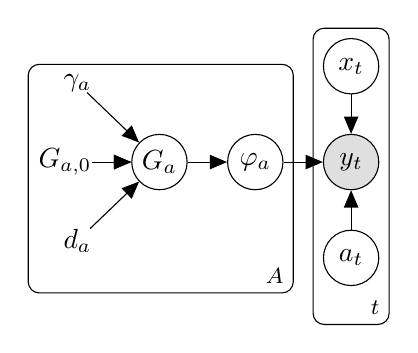
\begin{tikzpicture}
	% Nodes
	% Return y
	\node[obs] (y-t) {$y_{t}$};
	% Action a
	\node[latent, below=0.5 of y-t] (a-t) {$a_t$};
	% Context x
	\node[latent, above=0.5 of y-t]  (x-t) {$x_t$};
	% Nonparametric parameters
	\node[latent, left=0.5 of y-t, xshift=0cm] (varphi-a) {$\varphi_{a}$};
	% Nonparametric distribution
	\node[latent, left=0.5 of varphi-a, xshift=0cm] (G-a) {$G_{a}$};
	
	% Hyperparameters
	\node[const, left=0.5 of G-a, yshift=-1.0cm] (d-a) {$d_{a}$} ;
	\node[const, left=0.5 of G-a, yshift=0.0cm]  (G-a0) {$G_{a,0}$} ;
	\node[const, left=0.5 of G-a, yshift=1.0cm] (gamma-a) {$\gamma_{a}$} ;
	
	% Edges
	% Hyperparameters to distribution
	\edge {gamma-a,G-a0} {G-a} ;
	\edge {d-a,G-a0} {G-a} ;
	% Connect distribution to parameters
	\edge {G-a} {varphi-a} ;
	% Connect parameters, context and arm to observation
	\edge {varphi-a,x-t,a-t} {y-t} ;
	
	% Plates
	% Over time
	\plate {t} {(a-t)(x-t)(y-t)} {$t$} ;
	% Over each arm
	\plate {a}{
		(d-a)(gamma-a)(G-a0) % hyperparameters
		(G-a) % distribution
		(varphi-a) % parameters
	} {$A$} ;
\end{tikzpicture}
		\caption{The Bayesian nonparametric mixture bandit, as a probabilistic graphical model.}
		\label{fig:pgm_nonparametric_bandit}
		\vspace*{-4ex}
	\end{center}
\end{figure}

By characterizing each arm of the bandit with a different nonparametric model, we enjoy full flexibility to estimate each per-arm distribution independently, covering MAB cases with distinct reward model classes per-arm. This setting is a very powerful extension of the MAB problem, which has not attracted interest so far, yet can circumvent model misspecification.

At every interaction of the MAB agent with the environment, reward $y_{t,a_t}$ is \iid drawn from a context dependent unknown distribution $Y_{t,a_t}\sim p(Y|a_t,x_t,\thetastar)$ of the played arm $a_t$, which we here approximate via Bayesian nonparametric mixture models~\citep{b-Ghosal2017}.

Specifically, we model context-conditional reward densities with nonparametric Gaussian mixtures per-arm, \ie
\begin{align}
Y_{t,a} \sim p(Y|a,x_t,\varphi_a) &= \sum_{k=1}^{K_a} \frac{n_{a,k}-d_a}{n_a+\gamma_a} \cdot \N{Y|x_{t}^\top w_{a,k}, \sigma_{a,k}^2} \nonumber \\
& \qquad + \frac{\gamma_a+K_ad_a}{n_a+\gamma_a} \N{Y|x_{t}^\top w_{a,k_{new}}, \sigma_{a,k_{new}}^2} \;,
\label{eq:nonparametric_Gaussian_mixture}
\end{align}
where the number of mixands $K_a$ is determined by independent per-arm Pitman-Yor processes: $n_{a,k}$ refers to the rewards observed after playing arm $a$ that are assigned to mixture $k$, and $n_a=\sum_{k=1}^{K_a}n_{a,k}$.
After $n_{a}$ observations for arm $a$, there are $K_a$ already `\textit{seen}' mixtures, and a probability of $\frac{\gamma_a+K_ad_a}{n_a+\gamma_a}$ of incorporating a new mixand $k_{new}$ to the mixture.

Eqn.~\eqref{eq:nonparametric_Gaussian_mixture} describes per-arm nonparametric Gaussian mixture densities, with a Pitman-Yor nonparametric prior as described in Eqn.~\eqref{eq:pitman_yor_mixture}.
Each per-arm distribution is modeled independently with per-arm specific parameterizations: $d_a$, $\gamma_a$, $\varphi_{a,k}=\{w_{a,k}, \sigma_{a,k}^2 \}$, for $k={1,\cdots, K_a}$. 

The proposed contextual nonparametric model relies on leveraging context-conditional Gaussian models (with an expected value that is linearly dependent on the context at time $t$, \ie $\mu_{t,a,k}=x_t^\top w_{a,k}$), and extending them to a potentially infinite mixture.
As the number of mixands $K_a$ grows, the nonparametric distribution can be non-linear in the context.

With the proposed per-arm nonparametric mixture of Gaussian densities, we make a very flexible reward model assumption that automatically adjusts to the observed data: we are nonparametrically estimating complex, unknown per-arm continuous reward densities.
We leverage the well known linear Gaussian model and allow for the nonparametric model to accommodate as many mixands as necessary to best describe the observed bandit data.

The proposed Bayesian nonparametric model provides a flexible approach to density estimation, which can arbitrarily approximate continuous distributions. 
The Bayesian nonparametric literature has already established strong convergence results on the density estimation properties of these models: for a wide class of continuous distributions, the nonparametric posterior converges to the true data-generating density, under mild regularity conditions~\citep{j-Ghosal1999, j-Lijoi2004, j-Tokdar2006, j-Ghosal2007, j-Bhattacharya2010, j-Pati2013}.

In theory, the proposed Bayesian nonparametric model is on an infinite-dimensional parameter space (\ie the Pitman-Yor process can accommodate countably infinite mixands).
In practice, the model as in Eqn.~\eqref{eq:nonparametric_Gaussian_mixture} will use a finite subset of the available parameter dimensions to explain a finite sample of observations: \ie it sets the number of mixands per-arm $K_a$ according to the observed per-arm rewards.
Consequently, the effective complexity of the resulting model (\ie the dimensionality $K_a$ in Eqn.~\eqref{eq:nonparametric_Gaussian_mixture}) adapts to the observed data.

\subsection{Nonparametric context-conditional Gaussian mixture model posterior}
\label{ssec:nonparametric_posterior_update}

We now derive the procedure for inference of the per-arm, context-dependent reward posterior density of the proposed Bayesian nonparametric Gaussian mixture model.
As outlined in Section~\ref{ssec:background_nonparametric_mixture_model}, we rely on auxiliary latent variables per-arm $z_{1:n_a}$, and implement a Gibbs sampler that iterates between sampling mixture assignments $z_{1:n_a}$, and updating the emission distribution parameter posterior $G_{n_{a,k}}(\varphi_{a,k})$ for each arm and mixture. 

We start with the derivation of the parameter posteriors.
Per-arm and per-mixand emission distributions in Eqn.~\eqref{eq:nonparametric_Gaussian_mixture} are context-conditional Gaussian densities
\begin{equation}
\N{Y|x^\top w_{a,k}, \sigma_{a,k}^2} \; ,
\end{equation}
where $x^\top w_{a,k}$ and $\sigma_{a,k}^2$ are the means and variances, respectively, of the $k$-th mixand of arm $a$ in round $t$.
The conjugate prior of each of the mixands is a Normal-inverse Gamma,
\begin{equation}
G_{a,0}(\varphi_a) = \NIG{w_a, \sigma_a^2 |U_{a,0}, V_{a,0},\alpha_{a,0}, \beta_{a,0}} \;, 
\end{equation}
with hyperparameters $\varPhi_{a,0}=\{U_{a,0}, V_{a,0},\alpha_{a,0}, \beta_{a,0}\}$.

After observing rewards $y_{1:n}$, and conditioned on the auxiliary assignment variables $z_{1:n_a}$, the posteriors of per-arm and mixand parameters $\varphi_{a,k}$ follow a Normal-inverse Gamma distribution with updated hyperparameters $\varPhi_{a,k,n_{a,k}}$:
\begin{align}
G_{a,n_{a,k}}(\varphi_{a,k}) &=\NIG{w_{a,k}, \sigma_{a,k}^2 |\varPhi_{a,k,n_{a,k}}} \;, \\
\varPhi_{a,k,n_{a,k}}& =\{U_{a,k,n_{a,k}}, V_{a,k,n_{a,k}},\alpha_{a,k,n_{a,k}}, \beta_{a,k,n_{a,k}} \} \;, \nonumber
\end{align}
that depend on the number $n_{a,k}$ of rewards observed after playing arm $a$ that are assigned to mixand $k$. Specifically,
\begin{equation}
\begin{cases}
V_{a,k,n_{a,k}}^{-1} = x_{1:n} R_{a,k} x_{1:n}^\top + V_{a,0}^{-1} \;,\\
U_{a,k,n_{a,k}}= V_{a,k,n_{a,k}} \left( x_{1:n} R_{a,k} y_{1:n} + V_{a,0}^{-1} U_{a,0}\right) \;, \\
\alpha_{a,k,n_{a,k}} = \alpha_{a,0} + \frac{1}{2} \tr{R_{a,k}} \;, \\
\beta_{a,k,n_{a,k}} = \beta_{a,0} + \frac{1}{2}\left(y_{1:n}^\top R_{a,k}y_{1:n} \right) + \frac{1}{2}\left( U_{a,0}^\top V_{a,0}^{-1} U_{a,0} - U_{a,k,n_{a,k}}^\top V_{a,k,n_{a,k}}^{-1} U_{a,k,n_{a,k}} \right) \; ,
\end{cases}
\label{eq:posterior_hyperparameters}
\end{equation}
where $R_{a,k}\in\Real^{n_a\times n_a}$ is a sparse diagonal matrix with elements $\left[R_{a,k}\right]_{i,i}=\mathds{1}[a_i=a,z_i=k]$ for $i=\{0,\cdots, n_a\}$, and $n_{a}=\sum_{k=1}^{K_a} n_{a,k}$ is the number of rewards observed after playing arm $a$. The number of mixands per-arm $K_a$ of the bandit is independently drawn from its own Pitman-Yor process. Note that the above expression can be computed sequentially as data are observed for the played arm.

The predictive emission distribution after marginalization of the parameters $\varphi_{a,k}$, needed for solving Eqn.~\eqref{eq:gibbs_mixture_assignment}, follows a conditional Student-t distribution
\begin{align}
p_{a,k}(Y|a,x,\varPhi_{a,k,,n_{a,k}}) &= \T{Y|\nu_{a,k,n_{a,k}}, m_{a,k,n_{a,k}}, r_{a,k,n_{a,k}}} \;, \nonumber \\
\text{with } \varPhi_{a,k,,n_{a,k}} &=
\begin{cases}
\nu_{a,k,n_{a,k}}=2\alpha_{a,k} \;, \\
m_{a,k,n_{a,k}} = x^\top U_{a,k} \;, \\
r_{a,k,n_{a,k}}^2 = \frac{\beta_{a,k}}{\alpha_{a,k}} (1+x^\top V_{a,k} x) \;.
\end{cases}
\label{eq:marginalized_predictive_emission_univariate}
\end{align}
The hyperparameters $\varPhi_{a,k,,n_{a,k}}=\{\nu_{a,k,n_{a,k}}, m_{a,k,n_{a,k}}, r_{a,k,n_{a,k}}\}$ above are those of the prior $\varPhi_{a,0}$, or the posterior $\varPhi_{a,k,n_{a,k}}$, depending on whether the predictive density refers to a `\textit{new}' mixand $k_{new}$ with $n_{a,k=k_{new}}=0$, or a `\textit{seen}' mixand $k$, for which $n_{a,k}\geq0$ observations have been already assigned to, respectively.

Similarly, the likelihood of a set of rewards assigned to per-arm mixand $k$, $Y_{a,k}=y_{1:n}\cdot \mathds{1}[a_n=a,z_n=k]$, given their associated contexts $X_{a,k}=x_{1:n} \cdot \mathds{1}[a_n=a,z_n=k]$, follows the matrix t-distribution
\begin{align}
&p(Y_{a,k}|X_{a,k},X_{\backslash a,k},Y_{\backslash a,k},\varPhi_{a,k}) = \MT{Y_{a,k}|\nu_{Y_{a,k}}, M_{Y_{a,k}}, \Psi_{Y_{a,k}}, \Omega_{Y_{a,k}}} \; , \nonumber  \\
\text{with }&\begin{cases}
\nu_{Y_{a,k}}=2 \alpha_{a,k} \;,\\
M_{Y_{a,k}}= X_{a,k}^\top U_{a,k} \;, \\
\Psi_{Y_{a,k}} = I_{n_{a,k}} + X_{a,k}^\top V_{a,k} X_{n_{a,k}} \;,\
\Omega_{Y_{a,k}} = 2 \beta_{a,k} \;.
\end{cases}
\label{eq:marginalized_predictive_emission_multivariate}
\end{align}

With parameter posteriors as in Eqns.~\eqref{eq:marginalized_predictive_emission_univariate} and~\eqref{eq:marginalized_predictive_emission_multivariate}, we implement a Gibbs sampler to infer the mixture assignments $z_{1:n}$, based on the assignment probabilities described in Eqn.~\eqref{eq:gibbs_mixture_assignment}, for per-arm already drawn mixture components $k_a\in\{1, \cdots, K_a\}$, and a new `\textit{unseen}' mixand $k_{a,new}$. Therefore, the proposed Gibbs sampler adjusts the nonparametric posterior's complexity (\ie number of mixands $K_a$) according to the observed per-arm rewards distribution.

\subsection{Nonparametric Gaussian mixture model based Thompson sampling}
\label{ssec:nonparametric_thompson_sampling}

We leverage the nonparametric context-conditional Gaussian mixture model described above, and combine it with a posterior sampling MAB policy, \ie Thompson sampling~\citep{j-Russo2018}. The proposed Thompson sampling technique for contextual bandits with nonparametric Gaussian mixture reward models is presented in Algorithm~\ref{alg:nonparametric_ts}.

%Nonparametric TS
\vspace*{-2ex}
\begin{algorithm}
	\caption{Nonparametric Gaussian mixture model based Thompson sampling}
	\label{alg:nonparametric_ts}
	\begin{algorithmic}[1]
		\STATE {\bfseries Input:} Number of arms $|\A|$
		\STATE {\bfseries Input:} Per-arm hyperparameters $d_a$, $\gamma_a$, $\varPhi_{a,0}$
		\STATE {\bfseries Input:} Gibbs convergence criteria $\epsilon$, $Gibbs_{max}$ 
		\STATE $\HH_1=\emptyset$
		\FOR{$t=1, \cdots, T$}
		\STATE Receive context $x_{t}$
		\FOR{$a=1, \cdots, |\A|$}
		\STATE Draw parameters from the posterior \\ $\hspace*{2ex}\varphi_{a,k}^{(t)} \sim G_{a,k,n_{a,k}}(\varPhi_{a,k}), \forall k$, as in Eqn.~\eqref{eq:posterior_hyperparameters}
		\STATE Compute $\mu_{t,a}(x_{t},\varphi_{a}^{(t)})$ as in Eqn.~\eqref{eq:nonparametric_expected_reward}
		\ENDFOR
		\STATE Play arm $a_{t}=\argmax_{a^\prime \in \A} \mu_{t,a^\prime}(x_{t},\varphi_{a^\prime}^{(t)})$
		\STATE Observe reward $y_{t}$
		\STATE $\HH_{1:t}=\HH_{1:t-1} \cup \left\{x_{t}, a_{t}, y_{t}\right\}$
		\WHILE{NOT Gibbs convergence criteria}
		\STATE Update mixture assignments $z_{1:n}$ based on Eqn.~\eqref{eq:gibbs_mixture_assignment}
		\STATE Compute sufficient statistics $n_{a,k}$
		\STATE Update parameter posteriors $\varPhi_{a,k,n_{a,k}}$ based on Eqn.~\eqref{eq:posterior_hyperparameters}
		\ENDWHILE
		\ENDFOR
	\end{algorithmic}
\end{algorithm}
\vspace*{-2ex}

At each interaction with the world, the proposed Thompson sampling decides which arm to play next based on a random parameter sample, drawn from the posterior nonparametric distribution updated with all the information available at time $t$.

The parameters' posterior distributions for the proposed nonparametric Gaussian mixture model are presented in Section~\ref{ssec:nonparametric_posterior_update}.
Specifically, for nonparametric models as in Eqn~\eqref{eq:nonparametric_Gaussian_mixture}, one draws per-arm and per-mixand Gaussian parameters $\varphi_{a,k}$ from the posterior distributions with updated hyperparameters $\varPhi_{a,k,n_{a,k}}$ in Eqn.~\eqref{eq:posterior_hyperparameters}, conditioned on the mixture assignments $z_{1:n}$ determined by the Gibbs sampler in Eqn.~\eqref{eq:gibbs_mixture_assignment}, with marginalized emission densities provided in Eqns.~\eqref{eq:marginalized_predictive_emission_univariate} and~\eqref{eq:marginalized_predictive_emission_multivariate}.

Given the inferred sufficient statistics of the assignments (\ie the counts $n_{a,k}$ of rewards observed for arm $a$ and assigned to mixand $k$), and the drawn posterior parameter samples $w_{a,k}^{(t)}$, one computes the expected reward for each arm of the nonparametric bandit, \ie

\begin{align}
\mu_{t,a}(x_{t},\varphi_{a}^{(t)})&=\sum_{k=1}^{K_a} \frac{n_{a,k}-d_a}{n_a+\gamma_a} \left(x_{t}^\top w_{a,k}^{(t)}\right) + \frac{\gamma_a+K_ad_a}{n_a+\gamma_a} \left(x_{t}^\top w_{a,k_{new}}^{(t)} \right)\; .
\label{eq:nonparametric_expected_reward}
\end{align}

The proposed Thompson sampling policy $\myPitilde{\Atilde_t|x_{t},\HH_{1:t-1}}$, with assumed per-arm nonparametric distribution $\ptilde(Y|a,x_t,\varphi_a)$ in Eqn~\eqref{eq:nonparametric_Gaussian_mixture}, picks the arm that maximizes the above expected reward, \ie
\begin{align}
\myPitilde{\Atilde_t|x_{t},\HH_{1:t-1}}&=\myPitilde{\Atilde_t|x_{t},\varphi_{a}^{(t)}} \nonumber \\
& =\myind{\Atilde_t=\argmax_{a^\prime \in \A} \mu_{t,a}\left(x_{t},\varphi_{a}^{(t)}\right)}\;, \varphi_{a}^{(t)} \sim p(\varphi_{a}|\HH_{1:t-1}) \;,
\end{align}
with updated hyperparameters for $\ptilde(\varphi_{a}|\HH_{1:t-1})$ as in Eqn.~\eqref{eq:posterior_hyperparameters}.

\subsubsection{Regret bound}
\label{sssec:nonparametric_thompson_sampling_regret_bound}

We leverage asymptotic posterior converge rates ---the rate at which the distance between two densities becomes small as the number of observation grows--- to asymptotically bound the regret of the proposed nonparametric Thompson sampling algorithm.

A Thompson sampling-based policy operates according to the probability of each arm being optimal. This probability is equivalent to the expectation with respect to the joint posterior distribution of the expected rewards given history and context, $p(\mu_t|x_{t},\HH_{1:t-1})$, of the optimal arm indicator function, \ie
\begin{align}
\myPi{p}{A_t|x_{t},\HH_{1:t-1}} &= \myProb{p}{A_t=\argmax_{a^\prime \in \A} \mu_{t,a^\prime}} =\eValue{p}{\myind{A_t=\argmax_{a^\prime \in \A}\mu_{t,a^\prime}}} \;.
\nonumber
\end{align}

Note that the indicator function $\myind{A_t=\argmax_{a^\prime \in \A}\mu_{t,a^\prime}}$ for each arm requires the posterior over all arms $a^\prime \in \A$ as input. That is, the posterior $p(\mu_t|x_{t},\HH_{1:t-1})$ is the joint posterior distribution over the expected rewards of all arms: $\mu_{t}=\{\mu_{t,a}\}, \forall a\in \A$; \ie it is a $|\A|$ dimensional multivariate distribution over all arms of the bandit.

We now present our first lemma, with the proof provided in Section~\ref{asec:nonparametric_thompson_sampling_regret_bound} of the Appendix, which is key to the cumulative regret theorem that follows.
\begin{lemma}
	The difference in action probabilities between two Thompson sampling policies, given the same history and context up to time $t$, is bounded by the total-variation distance $\delta_{TV}(p_t,q_t)$ between the posterior distributions of their expected rewards at time $t$, $p_t=p(\mu_{t}|x_t,\HH_{1:t-1})$ and $q_t=q(\mu_{t}|x_t,\HH_{1:t-1})$, respectively,
	\begin{equation}
	\myPi{p_t}{A_t=a} - \myPi{q_t}{A_t=a} \leq \delta_{TV}(p_t,q_t) \; .
	\nonumber
	\end{equation}
	\label{lemma:total_variation_bounds_diff_policies}
	The \textbf{total variation distance} $\delta_{TV}(p,q)$ between distributions $p$ and $q$ on a sigma-algebra $\mathcal{F}$ of subsets of the sample space $\Omega$ is defined as
	\begin{equation}
	\delta_{TV}(p, q) = \sup_{B \in \mathcal{F}} \left|p(B)-q(B)\right| \; ,
	\end{equation}
	which is properly defined for both discrete and continuous distributions (see details in Section~\ref{asec:nonparametric_thompson_sampling_regret_bound} of the Appendix).
\end{lemma}
We make use of Lemma~\ref{lemma:total_variation_bounds_diff_policies} to asymptotically bound the cumulative regret of the proposed Thompson sampling with Dirichlet process priors (\ie $d_a=0, \forall a$) and Gaussian emission distributions, for bandits with true reward densities that meet certain regularity conditions. 

\begin{theorem}
	The expected cumulative regret at time $T$ of a Dirichlet process Gaussian mixture model based Thompson sampling algorithm is asymptotically bounded by
	\begin{equation}
	R_T	\leq \mathcal{O}\left(|\A| \log^\kappa T \sqrt{T} \right) \; \text{ as } T \rightarrow \infty \; .
	\nonumber
	\end{equation}
	We use big-O notation $\mathcal{O}(\cdot)$ for the asymptotic regret bound, as it bounds from above the growth of the cumulative regret over time for large enough bandit interactions, \ie
	\begin{align}
	\lim_{T\rightarrow \infty} \frac{R_T}{|\A| \log^\kappa T \sqrt{T} } & \leq \mathcal{O}(1)\; .
	\end{align}
	We note that this bound holds both in a frequentist and Bayesian view of expected regret.
	\label{th:regret_bound}
\end{theorem}

The proof of Theorem~\ref{th:regret_bound}, provided in Section~\ref{asec:nonparametric_thompson_sampling_regret_bound} of the Appendix, consists of bounding the regret introduced by two factors: the first, related to the use of Thompson sampling (\ie a policy that does not know the true parameters of the reward distribution, but has knowledge of the true reward model class); and the second, a term that accounts for the convergence of the posterior of a nonparametric model to that of the true data generating distribution.

The logarithmic term $\log^\kappa T$ in the bound appears due to the convergence rate of the nonparametric density estimation, where the exponent $\kappa\geq 0$ depends on the tail behavior of the base measure and the priors of the Dirichlet process ---see Section \ref{asec:nonparametric_thompson_sampling_regret_bound} of the Appendix, and references therein, for details on density convergence and its impact on the exponent $\kappa\geq 0$.

\subsubsection{Computational complexity}
\label{sssec:nonparametric_thompson_sampling_computational_complexity}
The Gibbs sampler in the proposed nonparametric Thompson sampling (lines 14-18 within Algorithm~\ref{alg:nonparametric_ts}) is run $Gibbs_{steps}$ until a stopping criteria is met: either the model likelihood of the sampled chain is stable within an $\epsilon$ likelihood margin between steps, or a maximum number of iterations $Gibbs_{max}$ is reached.

As new rewards $y_{t,a_{t}}$ are acquired, updates to assignments $z_{t^\prime,a_{t}}$ are computed sequentially within the Gibbs sampler for $t^\prime=\{1,\cdots,t | a_{t^\prime}=a_{t}\}$; \ie only the posterior over the last played armed $a_{t}$ is recomputed. Since Eqn.~\eqref{eq:posterior_hyperparameters} can be sequentially computed for each per-arm observation, the computational cost of the Gibbs sampler grows with the number of available observation of the played arm. Therefore, the overall computational cost is upper-bounded by $\mathcal{O}(T \cdot Gibbs_{steps})$ per-interaction with the world, \ie per newly observed reward $y_{t,a_{t}}$.

Due to the sequential acquisition of observations in the bandit setting, and the need to only update the posterior for the played arm, the Gibbs sampler is \textit{warm-started} at each bandit interaction, and good convergence can be achieved in few iterations per observed reward. 
In practice, and because of the \textit{warm-start}, one can limit the number of Gibbs sampler iterations per-bandit interaction to upper-bound the algorithm's complexity to $O(T\cdot Gibbs_{max})$ per interaction, yet achieve satisfactory performance ---empirical evidence of this claim is provided in Section~\ref{sssec:evaluation_mixture_scenarios_baselines}.
Due to the \textit{warm-start}, the Gibbs sampler is run from a good starting point: the per-arm parameter space that describes all but this newly observed reward $y_{t,a_{t}}$.

We emphasize that we propose a Gibbs sampler that runs until convergence, but suggest to limit the number of Gibbs iterations as a practical recommendation with good empirical regret performance, yet upper-bounded $\mathcal{O}(T \cdot Gibbs_{max})$ computational complexity per MAB interaction with the environment.


\section{Evaluation}
\label{sec:evaluation}
% !TEX root = smc_bandits.tex
We empirically evaluate the proposed SMC-based Bayesian MAB framework
in non-stationary bandit scenarios
%\footnote{
%	Results in Appendix~\ref{assec:static_bandits_experiments_analytical}
%	validate the performance of SMC-based policies in stationary bandits.
%	We compare their performance to solutions based on analytically attainable posteriors
%	with Bernoulli and contextual linear Gaussian reward functions~\citep{ip-Kaufmann2012,ip-Garivier2011a,ic-Korda2013,ip-Agrawal2013a},
%	as well as for context-dependent binary rewards modeled with the logistic reward function~\cite{ic-Chapelle2011,j-Scott2015} ---Appendix~\ref{assec:static_bandits_experiments_logistic}.
%	Results showcase satisfactory performance across a wide range of stationary bandit parameterizations and sizes,
%	as SMC-based policies achieve the right exploration-exploitation tradeoff.
%}
with continuous, binary and discrete-categorical reward distributions.

Results in Appendix~\ref{assec:static_bandits_experiments_analytical}
validate the performance of SMC-based policies in stationary bandits.
We compare their performance to solutions based on analytically attainable posteriors
with Bernoulli and contextual linear Gaussian reward functions~\citep{ip-Kaufmann2012,ip-Garivier2011a,ic-Korda2013,ip-Agrawal2013a},
as well as for context-dependent binary rewards modeled with the logistic reward function~\cite{ic-Chapelle2011,j-Scott2015} ---Appendix~\ref{assec:static_bandits_experiments_logistic}.
Results showcase satisfactory performance across a wide range of stationary bandit parameterizations and sizes,
as SMC-based policies achieve the right exploration-exploitation tradeoff.

For results we present below, we simulate different parameterizations of dynamic linear models described in Section~\ref{ssec:linear_mixing_dynamics},
and present results for a variety of MAB environments with reward functions detailed in Sections~\ref{ssec:dynamic_bandits_gaussian},~\ref{ssec:dynamic_bandits_logistic} and~\ref{ssec:dynamic_bandits_categorical}.
Section~\ref{ssec:logged_data_bandits} illustrates
the ability of SMC-based bandit policies
to capture non-stationary trends in personalized news article recommendations.

The main evaluation metric is the cumulative regret of the bandit agent, as defined in Equation~\eqref{eq:mab_cumulative_regret},
with results averaged over 500 realizations.
We present results for SMC-based policies with $M=2000$ samples,
and provide an evaluation of the impact of $M$ in Appendix~\ref{asec:dynamic_bandits}.

\subsection{Non-stationary, linear Gaussian rewards}
\label{ssec:dynamic_bandits_gaussian}
% !TEX root = smc_bandits.tex
We simulate the following two-armed, contextual ($x_t\in\Real^2, \forall t$), linear Gaussian bandit:
\begin{equation}
\text{Scenario A}
\begin{cases}
	\vspace*{1ex}
	p(\theta_{t,a=0}|\theta_{t-1,a=0}): \\ \vspace*{1ex}
	\hspace*{10ex}\begin{pmatrix}
	\theta_{t,a=0,0}\\
	\theta_{t,a=0,1}\\
	\end{pmatrix} = \begin{pmatrix}
	0.9 & -0.1 \\
	-0.1 & 0.9 \\
	\end{pmatrix} \begin{pmatrix}
	\theta_{t-1,a=0,0}\\
	\theta_{t-1,a=0,1}\\
	\end{pmatrix} + \epsilon_{a=0} \;, \\ \vspace*{1ex}
	\hspace*{40ex} \text{where } \;  \epsilon_{a=0} \sim \N{\epsilon|0,0.01 \cdot\mathrm{I}},\\
	
	\vspace*{1ex}
	p(\theta_{t,a=1}|\theta_{t-1,a=1}): \\ \vspace*{1ex}
	\hspace*{10ex}\begin{pmatrix}
	\theta_{t,a=1,0}\\
	\theta_{t,a=1,1}\\
	\end{pmatrix} = \begin{pmatrix}
	0.9 & 0.1 \\
	0.1 & 0.9 \\
	\end{pmatrix} \begin{pmatrix}
	\theta_{t-1,a=1,0}\\
	\theta_{t-1,a=1,1}\\
	\end{pmatrix} + \epsilon_{a=1} \;, \\ \vspace*{1ex}
	\hspace*{40ex} \text{where } \;  \epsilon_{a=1} \sim \N{\epsilon|0,0.01 \cdot\mathrm{I}},\\
	
	p_a(Y|x,\theta_{t,a})=\N{Y|x^\top \theta_{t,a}, \sigma_a^2} \;.
\end{cases}
\label{eq:linear_mixing_dynamics_a}
\end{equation}

\begin{equation}
\text{Scenario B}
\begin{cases}
	\vspace*{1ex}
	p(\theta_{t,a=0}|\theta_{t-1,a=0}): \\ \vspace*{1ex}
	\hspace*{10ex}\begin{pmatrix}
	\theta_{t,a=0,0}\\
	\theta_{t,a=0,1}\\
	\end{pmatrix} = \begin{pmatrix}
	0.5 & 0.0 \\
	0.0 & 0.5 \\
	\end{pmatrix} \begin{pmatrix}
	\theta_{t-1,a=0,0}\\
	\theta_{t-1,a=0,1}\\
	\end{pmatrix} + \epsilon_{a=0} \;, \\ \vspace*{1ex}
	\hspace*{40ex} \text{where } \;  \epsilon_{a=0} \sim \N{\epsilon|0,0.01 \cdot\mathrm{I}},\\
	
	\vspace*{1ex}
	p(\theta_{t,a=1}|\theta_{t-1,a=1}): \\ \vspace*{1ex}
	\hspace*{10ex}\begin{pmatrix}
	\theta_{t,a=1,0}\\
	\theta_{t,a=1,1}\\
	\end{pmatrix} = \begin{pmatrix}
	0.9 & 0.1 \\
	0.1 & 0.9 \\
	\end{pmatrix} \begin{pmatrix}
	\theta_{t-1,a=1,0}\\
	\theta_{t-1,a=1,1}\\
	\end{pmatrix} + \epsilon_{a=1} \;, \\ \vspace*{1ex}
	\hspace*{40ex} \text{where } \;  \epsilon_{a=1} \sim \N{\epsilon|0,0.01 \cdot\mathrm{I}}, \\
	
	p_a(Y|x,\theta_{t,a})=\N{Y|x^\top \theta_{t,a}, \sigma_a^2} \;.
\end{cases}
\label{eq:linear_mixing_dynamics_b}
\end{equation}
 
The expected rewards driven by the dynamics of Equations~\eqref{eq:linear_mixing_dynamics_a} and~\eqref{eq:linear_mixing_dynamics_b} change over time,
inducing switches on the identity of the optimal arm.
%
For instance, for a given realization of Scenario A shown in Figure~\ref{fig:linear_mixing_dynamics_a_gaussian},
there is an optimal arm swap between time-instants $t=(300, 550)$, with arm 1 becoming the optimal for all $t\geq600$;
for a realization of Scenario B illustrated in Figure~\ref{fig:linear_mixing_dynamics_b_gaussian},
there is an optimal arm change around $t=100$, a swap around $t=600$,
with arm 1 becoming optimal again after $t\geq1600$.

Empirical results for SMC-based Bayesian policies in scenarios described by Equations~\eqref{eq:linear_mixing_dynamics_a} and~\eqref{eq:linear_mixing_dynamics_b}
are shown in Figures~\ref{fig:dynamic_bandits_linearGaussian_dknown} and \ref{fig:dynamic_bandits_linearGaussian_dunknown}.

% Linear Gaussian, known parameters
\begin{figure}[!h]
	\centering
	\begin{subfigure}[b]{0.45\textwidth}
		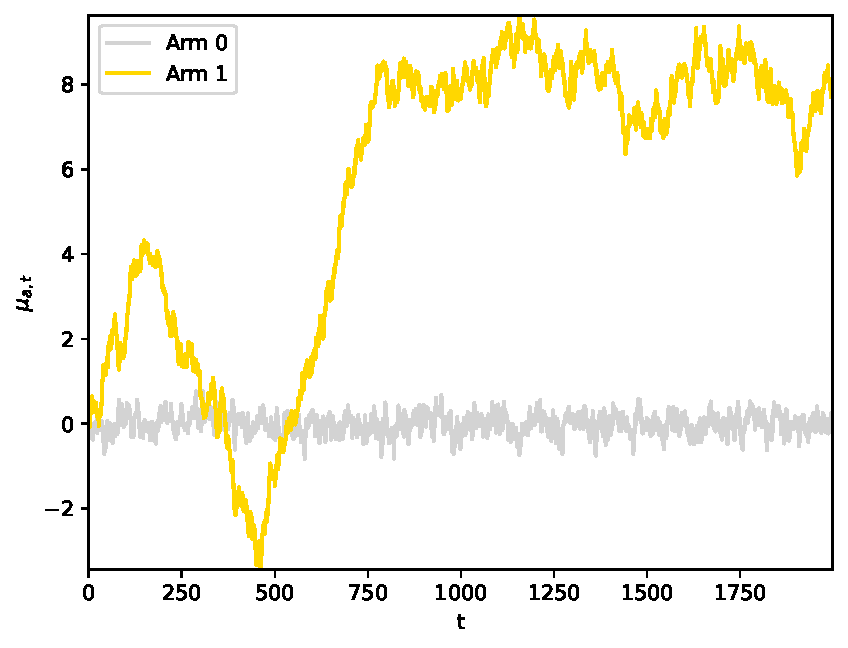
\includegraphics[width=\textwidth]{./fods_figs/dynamic/linearGaussian/dynamics_a}
		\caption{Expected per-arm rewards over time for Scenario A in Equation~\eqref{eq:linear_mixing_dynamics_a}.}
		\label{fig:linear_mixing_dynamics_a_gaussian}
	\end{subfigure}\qquad
	\begin{subfigure}[b]{0.45\textwidth}
		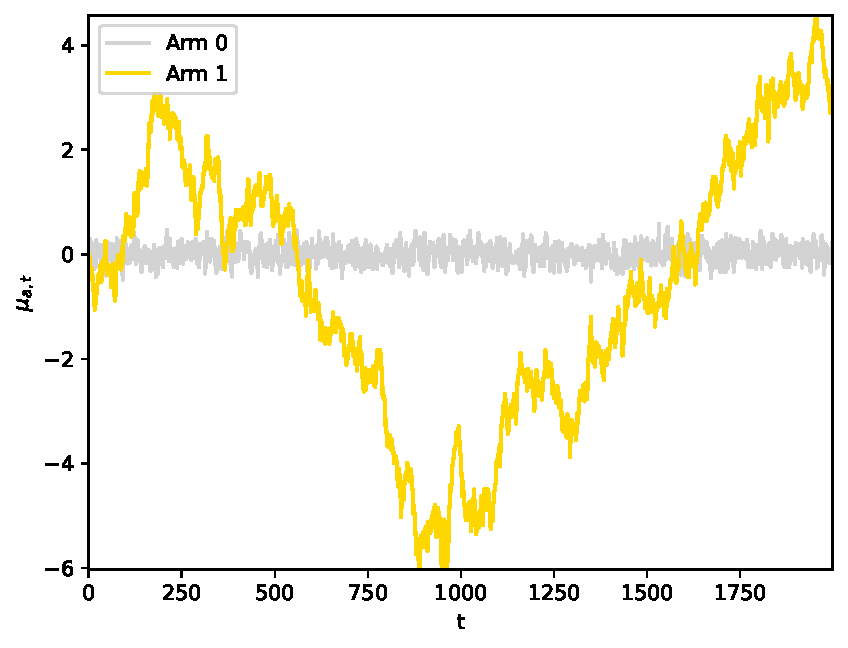
\includegraphics[width=\textwidth]{./fods_figs/dynamic/linearGaussian/dynamics_b}
		\caption{Expected per-arm rewards over time for Scenario B in Equation~\eqref{eq:linear_mixing_dynamics_a}.}
		\label{fig:linear_mixing_dynamics_b_gaussian}
	\end{subfigure}
	
	\begin{subfigure}[b]{0.47\textwidth}
		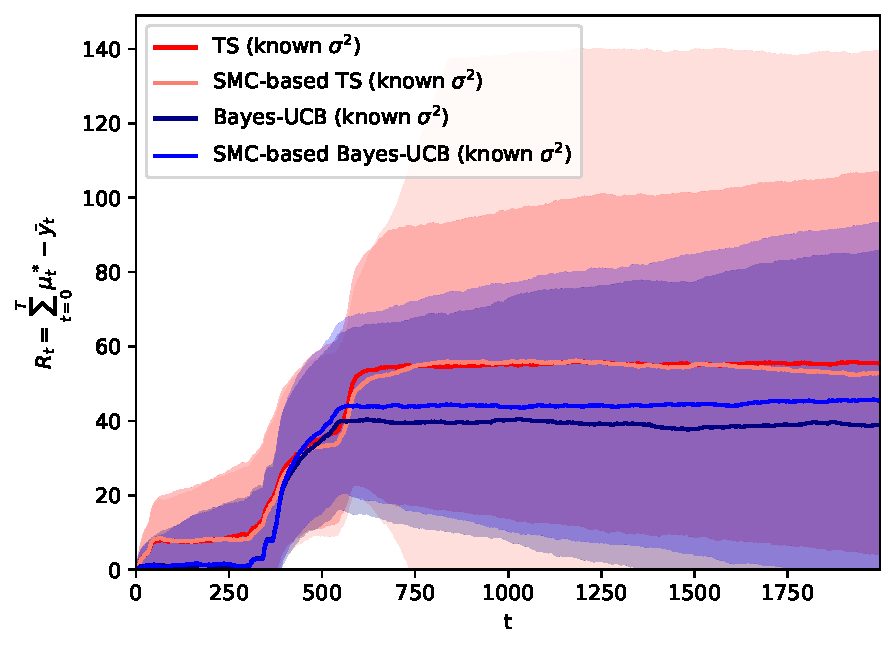
\includegraphics[width=\textwidth]{./fods_figs/dynamic/linearGaussian/a_M2000_cumulative_regret_dknown_knownsigma}
		\caption{Cumulative regret for SMC-based Bayesian policies in scenario A: known dynamic parameters.}
		\label{fig:dynamic_bandits_linearGaussian_a_cstatic_dknown_knownsigma}
	\end{subfigure}\qquad
	\begin{subfigure}[b]{0.47\textwidth}
		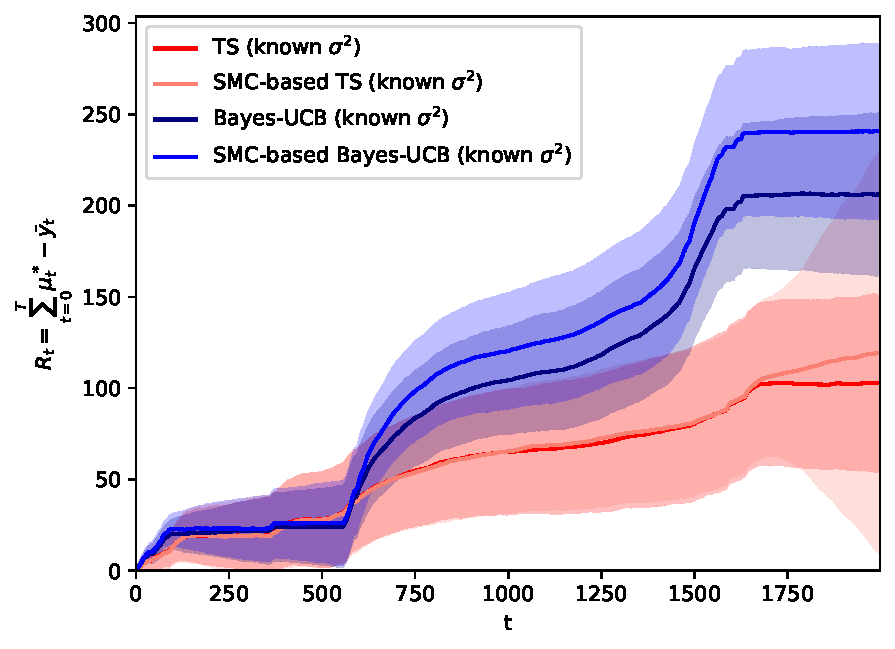
\includegraphics[width=\textwidth]{./fods_figs/dynamic/linearGaussian/b_M2000_cumulative_regret_dknown_knownsigma}
		\caption{Cumulative regret for SMC-based Bayesian policies in scenario B: known dynamic parameters.}
		\label{fig:dynamic_bandits_linearGaussian_b_cstatic_dknown_knownsigma}
	\end{subfigure}
	
	\caption{
		Mean regret (standard deviation shown as shaded region) in contextual, linear Gaussian bandit Scenarios A and B
		described in Equations~\eqref{eq:linear_mixing_dynamics_a}--\eqref{eq:linear_mixing_dynamics_b},
		when the bandit agent knows the latent dynamic parameterization.
		Notice how
		in Figures~\ref{fig:dynamic_bandits_linearGaussian_a_cstatic_dknown_knownsigma}--\ref{fig:dynamic_bandits_linearGaussian_b_cstatic_dknown_knownsigma}
		regret increases when the optimal arms swap
		(as shown in Figures~\ref{fig:linear_mixing_dynamics_a_gaussian}--\ref{fig:linear_mixing_dynamics_b_gaussian}).
		SMC-based policies successfully find the right exploration-exploitation tradeoff,
		with minimal additional regret incurred in comparison to their analytical alternatives. 
	}
	\label{fig:dynamic_bandits_linearGaussian_dknown}
\end{figure}

We study linear dynamics with Gaussian reward distributions with known parameters in Figure~\ref{fig:dynamic_bandits_linearGaussian_dknown},
of interest as it allows us to validate the SMC-based random measure in comparison to the optimal, closed-form posterior
---the Kalman filter~\cite{j-Kalman1960}---
under the assumption of known dynamic parameters.

We observe satisfactory cumulative regret performance in Figure~\ref{fig:dynamic_bandits_linearGaussian_dknown}:
\ie SMC-based Bayesian agents' cumulative regret is sublinear.
Policies that compute and use SMC random measure posteriors
incur in minimal regret loss 
in comparison to the optimal Kalman filter-based agent.
Namely, the shape of the regret curves of \textit{TS} and \textit{SMC-based TS}
(\textit{Bayes-UCB} and \textit{SMC based Bayes-UCB}, respectively) in Figure~\ref{fig:dynamic_bandits_linearGaussian_dknown} is equivalent,
with minimal differences in average cumulative regret when compared to the volatility across realizations.
Importantly, all policies are able to adapt to the changes over time of the identify of the optimal arm. 

We illustrate in Figure~\ref{fig:dynamic_bandits_linearGaussian_dunknown}
a more realistic scenario, where the dynamic parameterization is unknown to the bandit agent.

We observe in Figures~\ref{fig:dynamic_bandits_linearGaussian_a_cstatic_dknown_unknownsigma}--\ref{fig:dynamic_bandits_linearGaussian_b_cstatic_dknown_unknownsigma} that,
in the case of unknown reward variances ($\sigma_a^2, \forall a)$,
SMC-based policies perform comparably well.
In these cases,
the agents' reward model is not Gaussian,
but Student-t distributed, as per the marginalized posterior in Equation~\eqref{eq:t_posterior_mean}.
The regret loss associated with the uncertainty about $\sigma_a^2$ is minimal for SMC-based Bayesian agents,
and does not hinder the ability of the proposed SMC-based policies
to find the right exploration-exploitation balance:
\ie regret is sublinear, and the agents adapt to switches in the identity of the optimal arm.

We illustrate in Figures~\ref{fig:dynamic_bandits_linearGaussian_a_cstatic_dunknown}--\ref{fig:dynamic_bandits_linearGaussian_b_cstatic_dunknown}
the most realistic, yet challenging, non-stationary contextual Gaussian bandit case:
one where none of the parameters of the model are known.
In this case, the agent must sequentially learn both the underlying dynamics ($L_a,\Sigma_a; \forall a$)
and the conditional reward function's variance ($\sigma_a^2, \forall a)$,
in order to infer the posterior distribution over the latent, time-varying sufficient statistics of interest,
to enable informed sequential decision making.

Cumulative regret results in Figures~\ref{fig:dynamic_bandits_linearGaussian_a_cstatic_dunknown}--\ref{fig:dynamic_bandits_linearGaussian_b_cstatic_dunknown}
showcase a regret performance loss due to the need to learn all these unknown parameters.
We observe noticeable (almost linear) regret increases when the dynamics of the parameters swap the identity of the optimal arm.
However, SMC-based Thompson sampling and Bayes-UCB agents are able to learn the evolution of the dynamic latent parameters,
and the corresponding time-varying expected rewards,
with enough accuracy to attain good exploration-exploitation balance:
\ie sublinear regret curves indicate the agent identified and played the optimal arm repeatedly.
Figure~\ref{fig:dynamic_bandits_linearGaussian_a_cstatic_dunknown} is clear evidence of the SMC-based agents' ability to recover from linear to no-regret regimes.

\begin{figure}[!h]
	\centering
	\begin{subfigure}[b]{0.45\textwidth}
		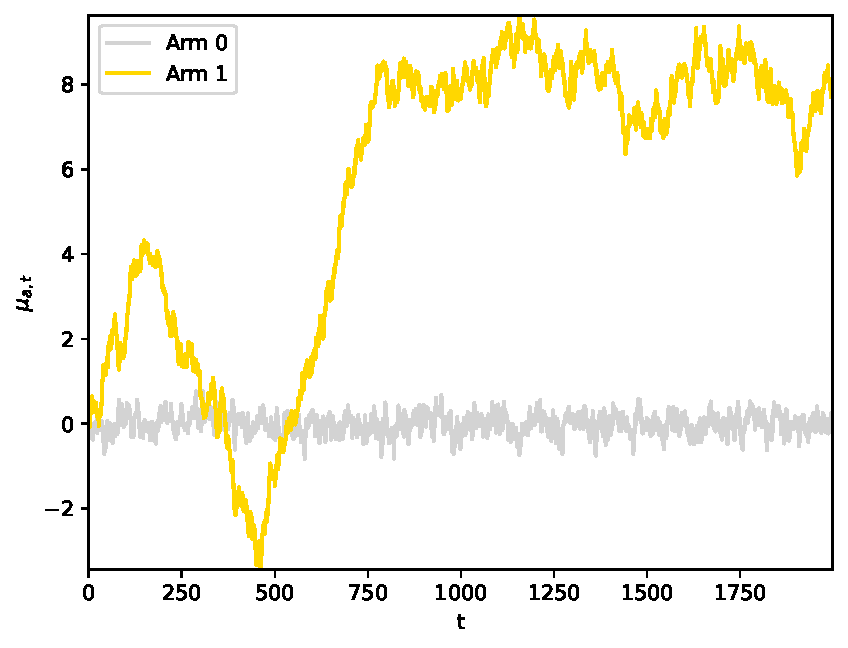
\includegraphics[width=\textwidth]{./fods_figs/dynamic/linearGaussian/dynamics_a}
		\caption{Expected per-arm rewards over time for Scenario A in Equation~\eqref{eq:linear_mixing_dynamics_a}.}
		\label{fig:linear_mixing_dynamics_a_gaussian_2}
	\end{subfigure}\qquad
	\begin{subfigure}[b]{0.45\textwidth}
		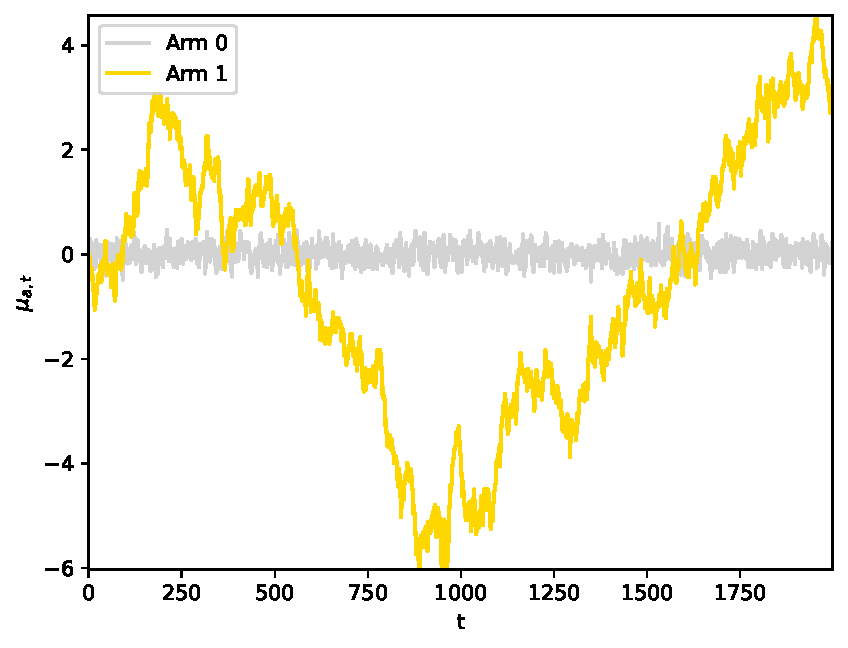
\includegraphics[width=\textwidth]{./fods_figs/dynamic/linearGaussian/dynamics_b}
		\caption{Expected per-arm rewards over time for Scenario B in Equation~\eqref{eq:linear_mixing_dynamics_a}.}
		\label{fig:linear_mixing_dynamics_b_gaussian_2}
	\end{subfigure}
	
	\begin{subfigure}[b]{0.47\textwidth}
		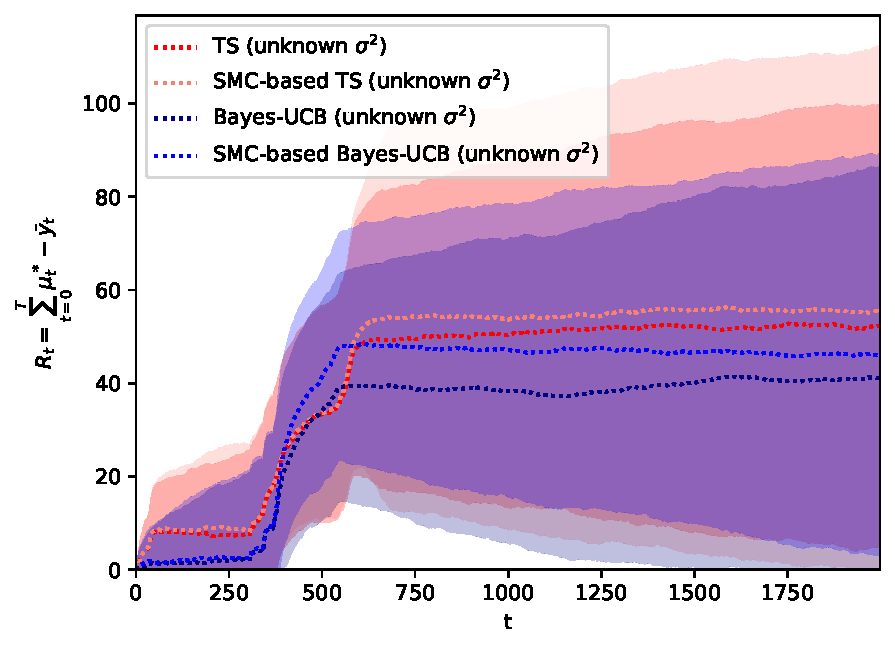
\includegraphics[width=\textwidth]{./fods_figs/dynamic/linearGaussian/a_M2000_cumulative_regret_dknown_unknownsigma}
		\caption{Cumulative regret for SMC-based Bayesian policies in scenario A: known dynamic parameters, unknown $\sigma_a, \forall a$.}
		\label{fig:dynamic_bandits_linearGaussian_a_cstatic_dknown_unknownsigma}
	\end{subfigure}\qquad
	\begin{subfigure}[b]{0.47\textwidth}
		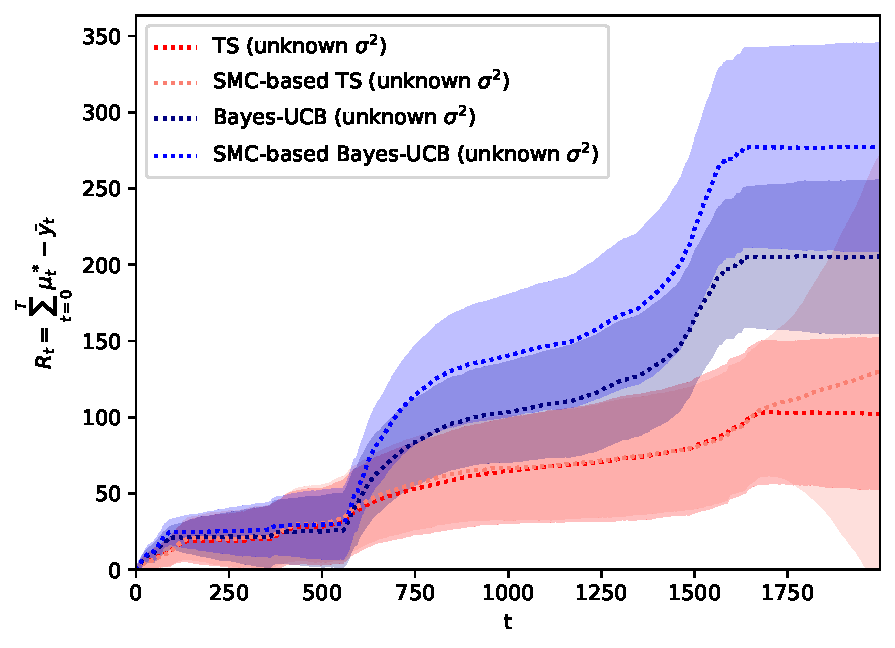
\includegraphics[width=\textwidth]{./fods_figs/dynamic/linearGaussian/b_M2000_cumulative_regret_dknown_unknownsigma}
		\caption{Cumulative regret for SMC-based Bayesian policies in scenario B: known dynamic parameters, unknown $\sigma_a, \forall a$.}
		\label{fig:dynamic_bandits_linearGaussian_b_cstatic_dknown_unknownsigma}
	\end{subfigure}
	
	\begin{subfigure}[b]{0.47\textwidth}
		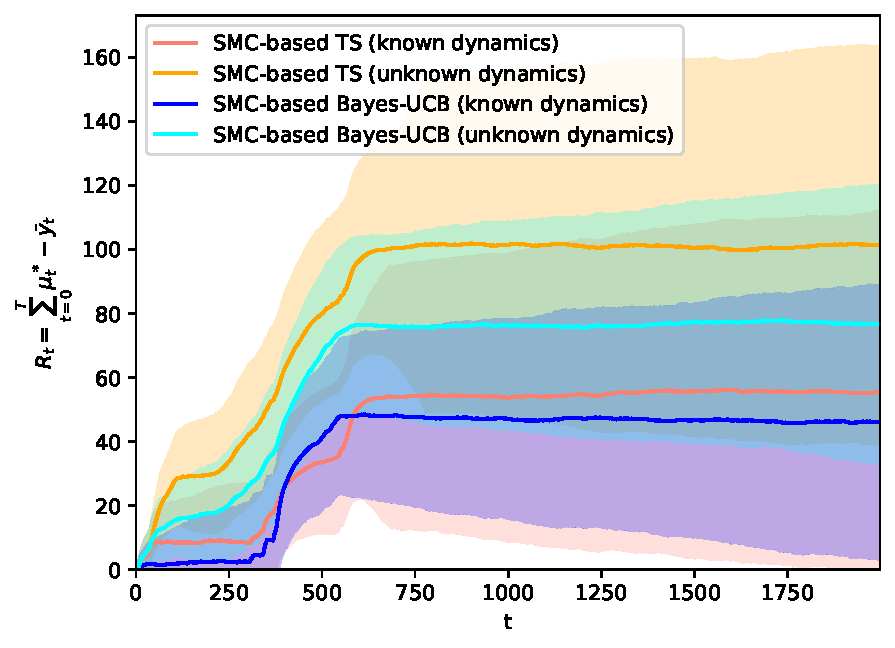
\includegraphics[width=\textwidth]{./fods_figs/dynamic/linearGaussian/a_M2000_cumulative_regret_dunknown}
		\caption{Cumulative regret for SMC-based Bayesian policies in scenario A: unknown dynamic parameters $L_a,\Sigma_a,\sigma_a^2, \forall a$.}
		\label{fig:dynamic_bandits_linearGaussian_a_cstatic_dunknown}
	\end{subfigure}\qquad
	\begin{subfigure}[b]{0.47\textwidth}
		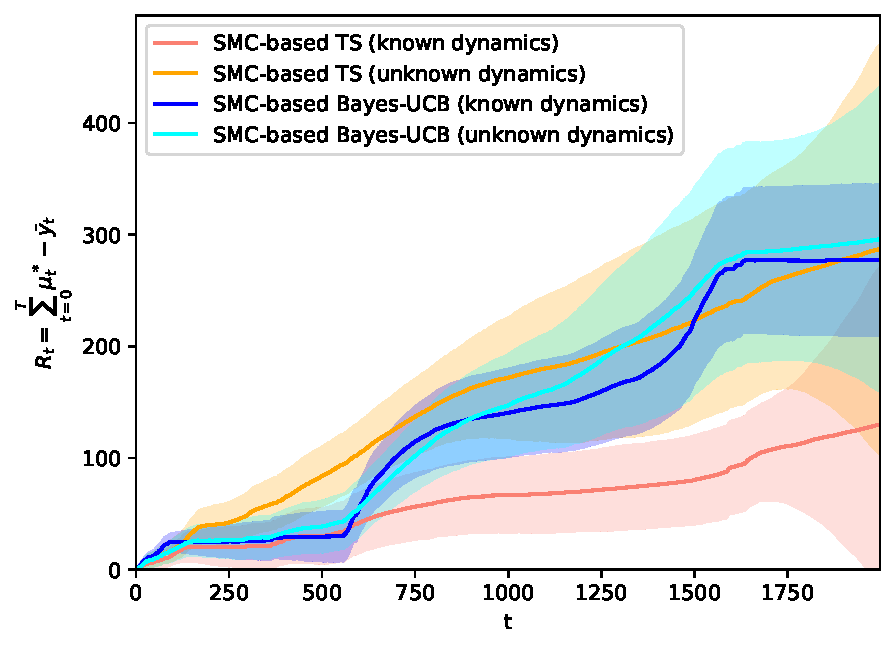
\includegraphics[width=\textwidth]{./fods_figs/dynamic/linearGaussian/b_M2000_cumulative_regret_dunknown}
		\caption{Cumulative regret for SMC-based Bayesian policies in scenario B: unknown dynamic parameters $L_a,\Sigma_a,\sigma_a^2, \forall a$.}
		\label{fig:dynamic_bandits_linearGaussian_b_cstatic_dunknown}
	\end{subfigure}
	\caption{
		Mean regret (standard deviation shown as shaded region) in contextual, linear Gaussian bandit Scenarios A and B
		described in Equations~\eqref{eq:linear_mixing_dynamics_a}--\eqref{eq:linear_mixing_dynamics_b},
		in the realistic setting of unknown dynamic parameters.
		Notice how
			in Figures~\ref{fig:dynamic_bandits_linearGaussian_a_cstatic_dknown_unknownsigma}--\ref{fig:dynamic_bandits_linearGaussian_b_cstatic_dunknown}
		the regret increases when the optimal arms swap
			(as shown in Figures~\ref{fig:linear_mixing_dynamics_a_gaussian_2}--\ref{fig:linear_mixing_dynamics_b_gaussian_2}).
		SMC-based policies find the right exploration-exploitation tradeoff even when the latent dynamic parameters are unknown.}
	\label{fig:dynamic_bandits_linearGaussian_dunknown}
\end{figure}


\clearpage
\subsection{Non-stationary, logistic rewards}
\label{ssec:dynamic_bandits_logistic}
% !TEX root = smc_bandits.tex
We here evaluate non-stationary, contextual, binary reward bandits.
We resort to the logistic reward function described in Equation~\eqref{eq:logistic_rewards},
with time-varying, latent parameter dynamics as described in the following scenarios:
\begin{equation}
\text{Scenario C}
\begin{cases}
\vspace*{1ex}
p(\theta_{t,a=0}|\theta_{t-1,a=0}): \\ \vspace*{1ex}
\hspace*{10ex}\begin{pmatrix}
\theta_{t,a=0,0}\\
\theta_{t,a=0,1}\\
\end{pmatrix} = \begin{pmatrix}
0.9 & -0.1 \\
-0.1 & 0.9 \\
\end{pmatrix} \begin{pmatrix}
\theta_{t-1,a=0,0}\\
\theta_{t-1,a=0,1}\\
\end{pmatrix} + \epsilon_{a=0} \;, \\ \vspace*{1ex}
\hspace*{40ex} \text{where } \;  \epsilon_{a=0} \sim \N{\epsilon|0,0.01 \cdot\mathrm{I}},\\

\vspace*{1ex}
p(\theta_{t,a=1}|\theta_{t-1,a=1}): \\ \vspace*{1ex}
\hspace*{10ex}\begin{pmatrix}
\theta_{t,a=1,0}\\
\theta_{t,a=1,1}\\
\end{pmatrix} = \begin{pmatrix}
0.9 & 0.1 \\
0.1 & 0.9 \\
\end{pmatrix} \begin{pmatrix}
\theta_{t-1,a=1,0}\\
\theta_{t-1,a=1,1}\\
\end{pmatrix} + \epsilon_{a=1}  \;, \\ \vspace*{1ex}
\hspace*{40ex} \text{where } \;  \epsilon_{a=1} \sim \N{\epsilon|0,0.01 \cdot\mathrm{I}},\\

p_a(Y|x,\theta_{t,a})=\frac{e^{y\cdot(x^\top\theta_{t,a}) }}{1+e^{(x^\top\theta_{t,a})}} \; .
\end{cases}
\label{eq:linear_mixing_dynamics_c}
\end{equation}

\begin{equation}
\text{Scenario D}
\begin{cases}
\vspace*{1ex}
p(\theta_{t,a=0}|\theta_{t-1,a=0}): \\ \vspace*{1ex}
\hspace*{10ex}\begin{pmatrix}
\theta_{t,a=0,0}\\
\theta_{t,a=0,1}\\
\end{pmatrix} = \begin{pmatrix}
0.5 & 0.0 \\
0.0 & 0.5 \\
\end{pmatrix} \begin{pmatrix}
\theta_{t-1,a=0,0}\\
\theta_{t-1,a=0,1}\\
\end{pmatrix} + \epsilon_{a=0}  \;, \\ \vspace*{1ex}
\hspace*{40ex} \text{where } \;  \epsilon_{a=0} \sim \N{\epsilon|0,0.01 \cdot\mathrm{I}},\\

\vspace*{1ex}
p(\theta_{t,a=1}|\theta_{t-1,a=1}): \\ \vspace*{1ex}
\hspace*{10ex}\begin{pmatrix}
\theta_{t,a=1,0}\\
\theta_{t,a=1,1}\\
\end{pmatrix} = \begin{pmatrix}
0.9 & 0.1 \\
0.1 & 0.9 \\
\end{pmatrix} \begin{pmatrix}
\theta_{t-1,a=1,0}\\
\theta_{t-1,a=1,1}\\
\end{pmatrix} + \epsilon_{a=1}  \;, \\ \vspace*{1ex}
\hspace*{40ex} \text{where } \;  \epsilon_{a=1} \sim \N{\epsilon|0,0.01 \cdot\mathrm{I}}, \\

p_a(Y|x,\theta_{t,a})=\frac{e^{y\cdot(x^\top\theta_{t,a}) }}{1+e^{(x^\top\theta_{t,a})}} \; .
\end{cases}
\label{eq:linear_mixing_dynamics_d}
\end{equation}

For bandits with logistic rewards,
there are no closed form posteriors;
hence, one needs to resort to approximations,
\eg a Laplace approximation as in~\citep{ic-Chapelle2011} for the stationary case.
However, there are no bandit algorithms for the non-stationary logistic scenarios described above.
%
On the contrary, SMC-based Bayesian policies can easily accommodate this setting,
by updating posterior random measures $p_M(\theta_{t}|\HH_{1:t})$ as in Algorithm~\ref{alg:sir-mab},
for both stationary (evaluated in Appendix~\ref{assec:static_bandits_experiments_logistic}) and non-stationary bandits we report here.

Figure~\ref{fig:dynamic_bandits_logistic} illustrates how
SMC-based Bayesian policies adapt to non-stationary optimal arm switches under contextual, binary reward observations,
achieving sublinear regret.
Results in Figures~\ref{fig:linear_mixing_dynamics_d_logistic}--\ref{fig:dynamic_bandits_d_logistic_cstatic}
also showcase how a bandit agent's regret suffers when learning unknown parameters of the latent dynamics.
%
Even though this is a particularly challenging problem,
presented evidence suggests that
SMC-based policies do learn the underlying latent dynamics from contextual binary rewards.

Notably, proposed policies are able to successfully identify which arm to play:
\ie both \textit{SMC-based TS and SMC-based UCB} ---with no dynamic parameter knowledge---
are able to flatten their regret
for $t\geq 650$ in Figure~\ref{fig:dynamic_bandits_c_logistic_cstatic} and
$t\geq 1750$ in Figure~\ref{fig:dynamic_bandits_d_logistic_cstatic}.

% Logistic results 
\begin{figure}[!h]
	\begin{subfigure}[b]{0.45\textwidth}
		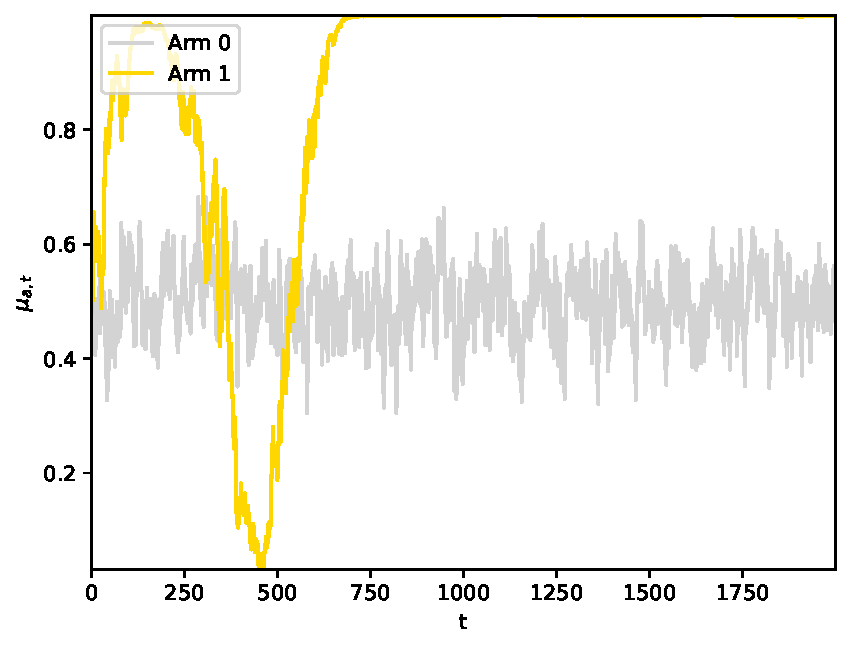
\includegraphics[width=\textwidth]{./fods_figs/dynamic/logistic/dynamics_c}
		\caption{Expected per-arm rewards over time for Scenario C in Equation~\eqref{eq:linear_mixing_dynamics_c}.
			Notice the early optimal arm change at $t\approx600$.
		}
		\label{fig:linear_mixing_dynamics_c_logistic}
	\end{subfigure}\qquad
	\begin{subfigure}[b]{0.45\textwidth}
		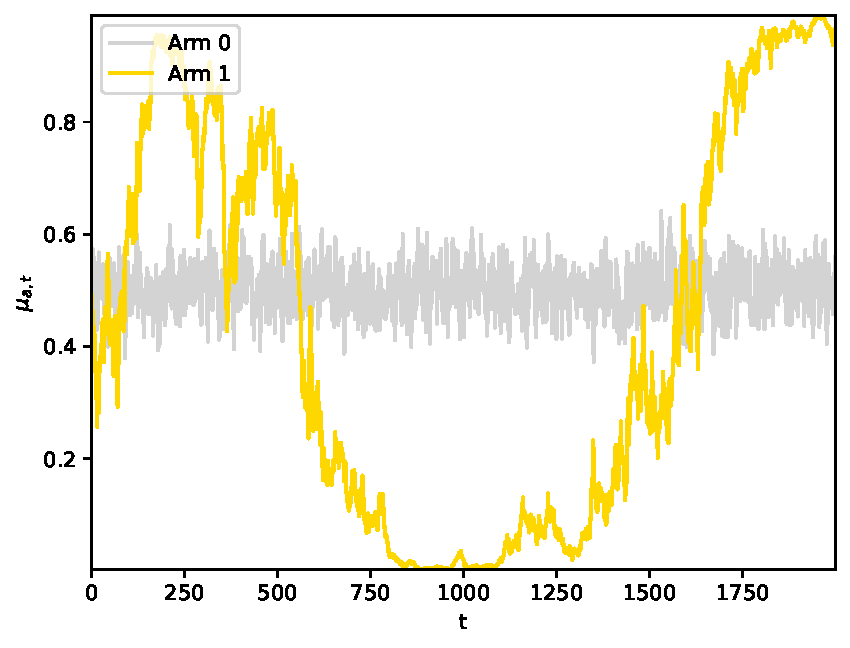
\includegraphics[width=\textwidth]{./fods_figs/dynamic/logistic/dynamics_d}
		\caption{Expected per-arm rewards over time for Scenario D in Equation~\eqref{eq:linear_mixing_dynamics_d}.
			Notice the late optimal arm change at $t\approx1650$.
		}
		\label{fig:linear_mixing_dynamics_d_logistic}
	\end{subfigure}
	
	\begin{subfigure}[b]{0.47\textwidth}
		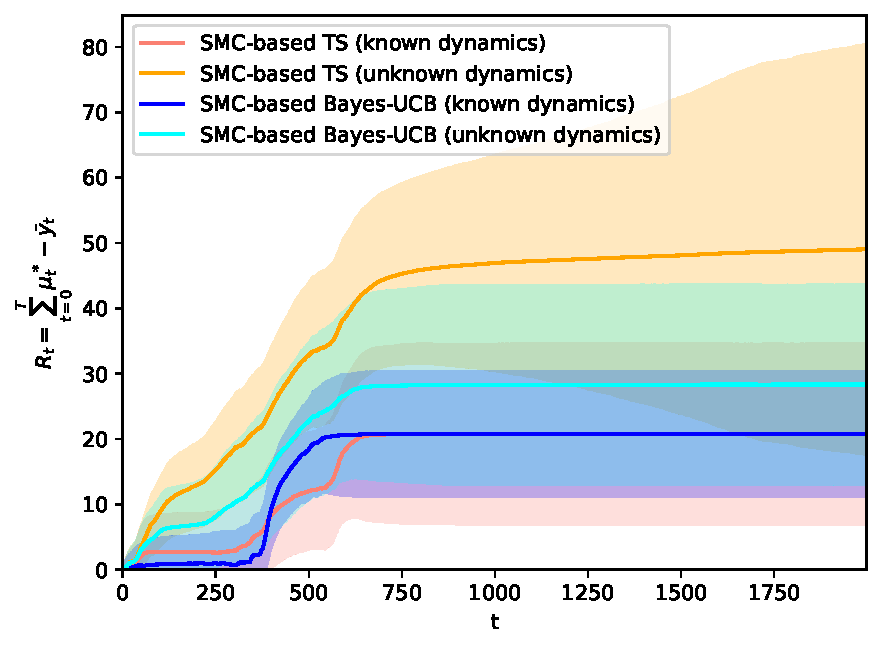
\includegraphics[width=\textwidth]{./fods_figs/dynamic/logistic/c_M2000_cumulative_regret_dunknown}
		\caption{Cumulative regret for SMC-based Bayesian policies in scenario C: known and unknown dynamic parameters.}
		\label{fig:dynamic_bandits_c_logistic_cstatic}
	\end{subfigure}\qquad
	\begin{subfigure}[b]{0.47\textwidth}
		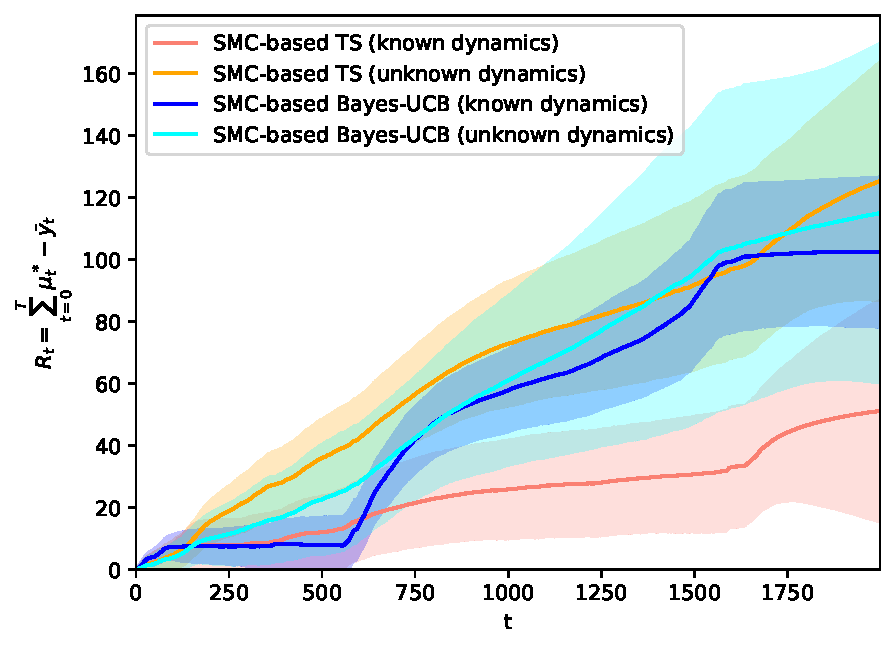
\includegraphics[width=\textwidth]{./fods_figs/dynamic/logistic/d_M2000_cumulative_regret_dunknown}
		\caption{Cumulative regret for SMC-based Bayesian policies in scenario D: known and unknown dynamic parameters.}
		\label{fig:dynamic_bandits_d_logistic_cstatic}
	\end{subfigure}
	\caption{
		Mean regret (standard deviation shown as shaded region) in contextual linear logistic dynamic bandit Scenarios C and D
		described in Equations~\eqref{eq:linear_mixing_dynamics_c}--\eqref{eq:linear_mixing_dynamics_d}.
		Notice the difference in early ($t\approx600$ in Scenario C) and late ($t\approx1650$ in Scenario D) optimal arm changes,
			as illustrated in Figures~\ref{fig:linear_mixing_dynamics_c_logistic}--\ref{fig:linear_mixing_dynamics_d_logistic},
		and their impact in regret,
			as showcased in Figures~\ref{fig:dynamic_bandits_c_logistic_cstatic}--\ref{fig:dynamic_bandits_d_logistic_cstatic}.
		SMC-based Bayesian policies adapt and find the right exploration-exploitation tradeoff.}
	\label{fig:dynamic_bandits_logistic}
\end{figure}


\clearpage
\subsection{Non-stationary, categorical rewards}
\label{ssec:dynamic_bandits_categorical}
% !TEX root = smc_bandits.tex
We evaluate SMC-based Bayesian policies in a bandit setting that remains elusive to state-of-the-art bandit algorithms:
non-stationary bandits with discrete-categorical, contextual rewards.
%
We simulate the following two- and three-armed categorical bandit scenarios,
where numerical rewards $Y=c$, for $c\in\{0,1,2\}$,
depend on a two-dimensional context $x_t\in\Real^2$,
with time-varying parameters $\theta_{a,c,t}$
obeying the following dynamics:

\begin{equation}
\text{Scenario E}
\begin{cases}
\vspace*{1ex}
p(\theta_{t,a=0,c}|\theta_{t-1,a=0,c})\;, \; \forall c \in \{0,1,2\}:\\ \vspace*{1ex}
\hspace*{10ex}\begin{pmatrix}
\theta_{t,a=0,c,0}\\
\theta_{t,a=0,c,1}\\
\end{pmatrix} = \begin{pmatrix}
0.9 & -0.1 \\
-0.1 & 0.9 \\
\end{pmatrix} \begin{pmatrix}
\theta_{t-1,a=0,c,0}\\
\theta_{t-1,a=0,c,1}\\
\end{pmatrix} + \epsilon_{a=0,c} \;, \\ \vspace*{1ex}
\hspace*{38ex} \text{where } \; \epsilon_{a=0,c} \sim \N{\epsilon|0,0.01 \cdot\mathrm{I}}, \\

\vspace*{1ex}
p(\theta_{t,a=1,c}|\theta_{t-1,a=1,c})\;, \; \forall c \in \{0,1,2\}:\\ \vspace*{1ex}
\hspace*{10ex}\begin{pmatrix}
\theta_{t,a=1,c,0}\\
\theta_{t,a=1,c,1}\\
\end{pmatrix} = \begin{pmatrix}
0.9 & 0.1 \\
0.1 & 0.9 \\
\end{pmatrix} \begin{pmatrix}
\theta_{t-1,a=1,c,0}\\
\theta_{t-1,a=1,c,1}\\
\end{pmatrix} + \epsilon_{a=1,c} \;, \\ \vspace*{1ex}
\hspace*{38ex} \text{where } \;  \epsilon_{a=1,c} \sim \N{\epsilon|0,0.01 \cdot\mathrm{I}},\\

p_a(Y=c|x,\theta_{t,a})=\frac{e^{(x^\top\theta_{t,a,c})}}{\sum_{c'=1}^C e^{(x^\top\theta_{t,a,c'})} } \; .
\end{cases}
\label{eq:linear_mixing_dynamics_e}
\end{equation}

\begin{equation}
\text{Scenario F}
\begin{cases}
\vspace*{1ex}
p(\theta_{t,a=0,c}|\theta_{t-1,a=0,c}) \;, \; \forall c \in \{0,1,2\}:\\ \vspace*{1ex}
\hspace*{10ex}\begin{pmatrix}
\theta_{t,a=0,c,0}\\
\theta_{t,a=0,c,1}\\
\end{pmatrix} = \begin{pmatrix}
0.9 & -0.1 \\
-0.1 & 0.9 \\
\end{pmatrix} \begin{pmatrix}
\theta_{t-1,a=0,c,0}\\
\theta_{t-1,a=0,c,1}\\
\end{pmatrix} + \epsilon_{a=0,c} \;, \\ \vspace*{1ex}
\hspace*{38ex} \text{where } \; \epsilon_{a=0,c} \sim \N{\epsilon|0,0.01 \cdot\mathrm{I}}, \\

\vspace*{1ex}
p(\theta_{t,a=1,c}|\theta_{t-1,a=1,c})\;, \; \forall c \in \{0,1,2\}:\\ \vspace*{1ex}
\hspace*{10ex}\begin{pmatrix}
\theta_{t,a=1,c,0}\\
\theta_{t,a=1,c,1}\\
\end{pmatrix} = \begin{pmatrix}
0.9 & 0.1 \\
0.1 & 0.9 \\
\end{pmatrix} \begin{pmatrix}
\theta_{t-1,a=1,c,0}\\
\theta_{t-1,a=1,c,1}\\
\end{pmatrix} + \epsilon_{a=1,c} \;, \\ \vspace*{1ex}
\hspace*{38ex} \text{where } \; \epsilon_{a=1,c} \sim \N{\epsilon|0,0.01 \cdot\mathrm{I}},\\

\vspace*{1ex}
p(\theta_{t,a=2,c}|\theta_{t-1,a=2,c})\;, \; \forall c \in \{0,1,2\}:\\ \vspace*{1ex}
\hspace*{10ex}\begin{pmatrix}
\theta_{t,a=2,c,0}\\
\theta_{t,a=2,c,1}\\
\end{pmatrix} = \begin{pmatrix}
0.9 & 0.1 \\
0.1 & 0.9 \\
\end{pmatrix} \begin{pmatrix}
\theta_{t-1,a=2,c,0}\\
\theta_{t-1,a=2,c,1}\\
\end{pmatrix} + \epsilon_{a=2,c} \;, \\ \vspace*{1ex}
\hspace*{38ex} \text{where } \; \epsilon_{a=2,c} \sim \N{\epsilon|0,0.01 \cdot\mathrm{I}},\\

p_a(Y=c|x,\theta_{t,a})=\frac{e^{(x^\top\theta_{t,a,c})}}{\sum_{c'=1}^C e^{(x^\top\theta_{t,a,c'})} } \; .
\end{cases}
\label{eq:linear_mixing_dynamics_f}
\end{equation}

These bandit scenarios accommodate a diverse set of expected reward dynamics,
for each realization of the noise processes $\epsilon_{a,c}, \forall a,c$,
and depending on the initialization of parameters $\theta_{0,a}$.
%
We illustrate per-arm, expected reward time-evolution for a realization
of the two-armed bandit Scenario E in Figure~\ref{fig:linear_mixing_dynamics_e_softmax},
and for the three-armed bandit Scenario F in Figure~\ref{fig:linear_mixing_dynamics_f_softmax}.

In all cases, expected rewards of each arm vary over time,
resulting in transient and recurrent swaps of the optimal arm's identity.
We show the corresponding cumulative regret of SMC-based Bayesian policies
in Figure~\ref{fig:dynamic_bandits_e_softmax_cstatic} for Scenario E,
and in Figure~\ref{fig:dynamic_bandits_f_softmax_cstatic} for Scenario F.

\begin{figure}[!ht]
	\centering
	\begin{subfigure}[b]{0.47\textwidth}
		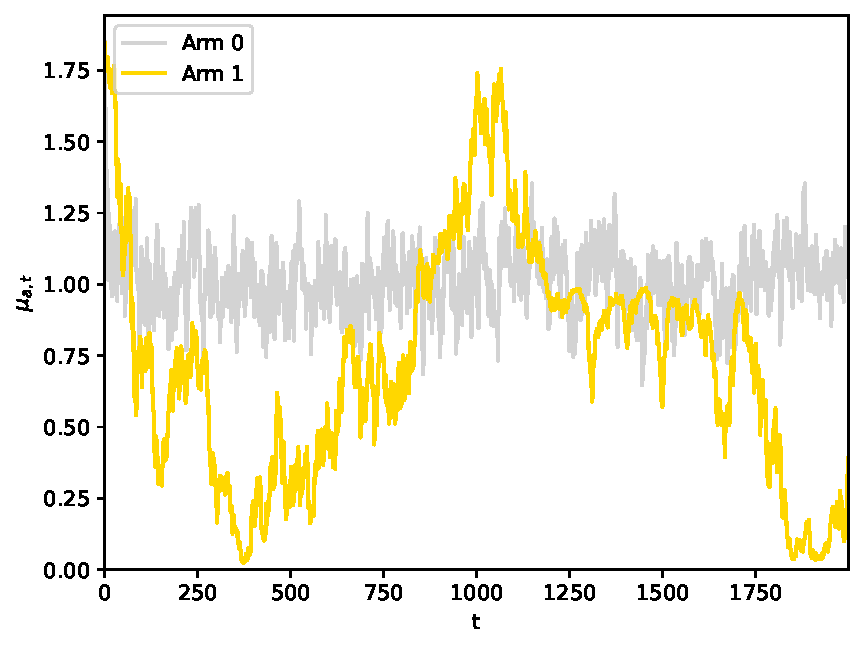
\includegraphics[width=\textwidth]{./fods_figs/dynamic/softmax/dynamics_e}
		\caption{Expected per-arm rewards over time for Scenario E in Equation~\eqref{eq:linear_mixing_dynamics_e}.
			Notice the optimal arm changes around $t\approx1000$.}
		\label{fig:linear_mixing_dynamics_e_softmax}%
	\end{subfigure}\qquad
	\begin{subfigure}[b]{0.47\textwidth}
		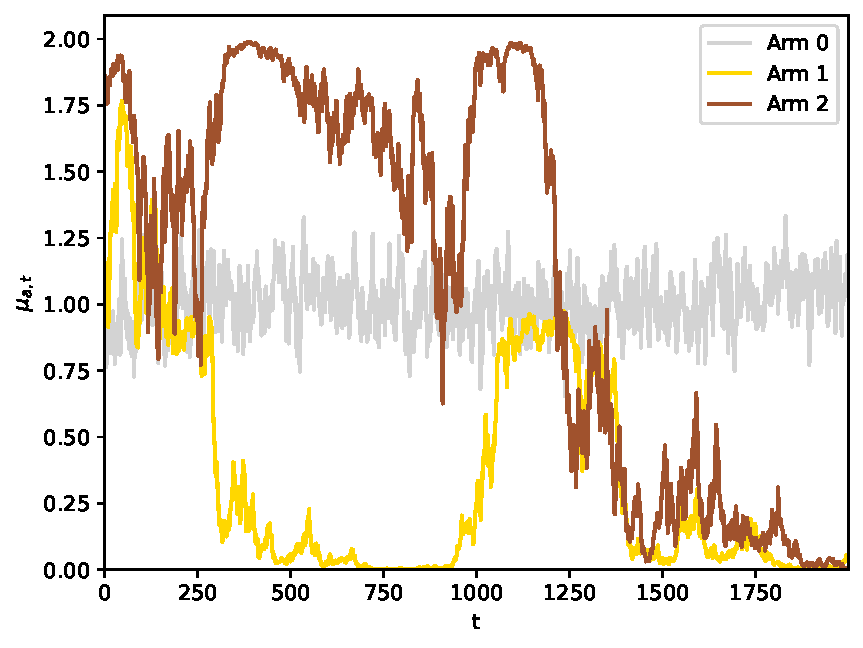
\includegraphics[width=\textwidth]{./fods_figs/dynamic/softmax/dynamics_f}
		\caption{Expected per-arm rewards over time for Scenario F in Equation~\eqref{eq:linear_mixing_dynamics_e}.
			Notice the optimal arm change around $t\approx1250$.}
		\label{fig:linear_mixing_dynamics_f_softmax}
	\end{subfigure} %
	
	\begin{subfigure}[b]{0.47\textwidth}
		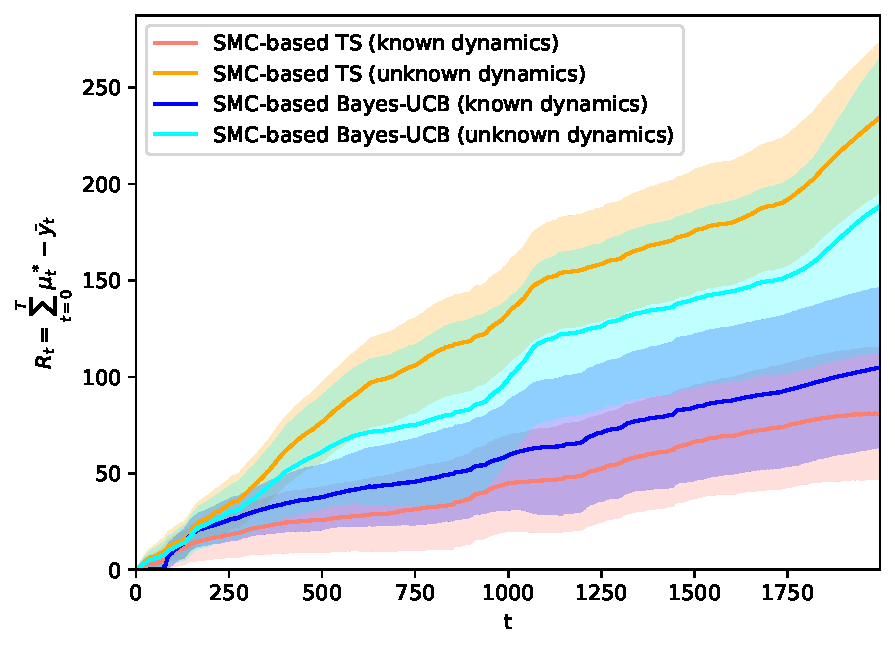
\includegraphics[width=\textwidth]{./fods_figs/dynamic/softmax/e_M2000_cumulative_regret_dunknown}
		\caption{Cumulative regret for SMC-based Bayesian policies in scenario E: known and unknown dynamic parameters.}
		\label{fig:dynamic_bandits_e_softmax_cstatic}%
	\end{subfigure}\qquad
	\begin{subfigure}[b]{0.47\textwidth}
		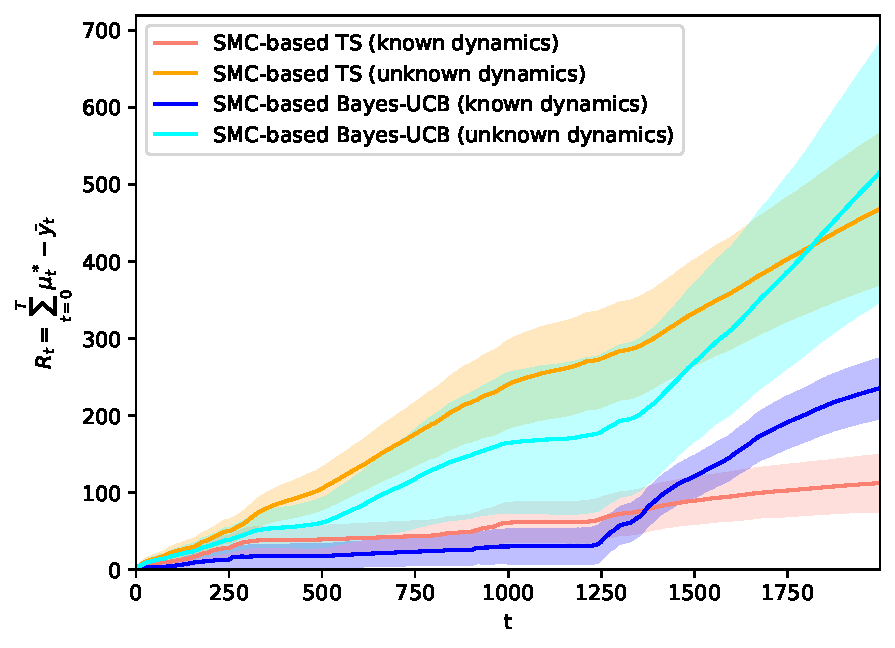
\includegraphics[width=\textwidth]{./fods_figs/dynamic/softmax/f_M2000_cumulative_regret_dunknown}
		\caption{Cumulative regret for SMC-based Bayesian policies in scenario F: known and unknown dynamic parameters.}
		\label{fig:dynamic_bandits_f_softmax_cstatic}%
	\end{subfigure}
	
	\caption{
		%Per-arm, expected reward evolution over time of two-armed contextual non-stationary categorical bandit Scenarios E and F
		%	described in Equations~\eqref{eq:linear_mixing_dynamics_e}--\eqref{eq:linear_mixing_dynamics_f}
		%	in Figures~\ref{fig:linear_mixing_dynamics_e_softmax}--\ref{fig:linear_mixing_dynamics_f_softmax}.
		Mean regret (standard deviation shown as shaded region) in contextual, non-stationary categorical bandit Scenarios E and F
		described in Equations~\eqref{eq:linear_mixing_dynamics_e}--\eqref{eq:linear_mixing_dynamics_f}.
		Notice how changes in per-arm expected rewards ($t\approx1750$ in Scenario E and $t>1250$ in Scenario F) 
		as illustrated in Figures~\ref{fig:linear_mixing_dynamics_e_softmax}--\ref{fig:linear_mixing_dynamics_f_softmax}
		impact regret
		as showcased in Figures~\ref{fig:dynamic_bandits_e_softmax_cstatic}--\ref{fig:dynamic_bandits_f_softmax_cstatic}.
		SMC-based Bayesian policies adapt to these changes and balance the exploration-exploitation tradeoff.
	}
	\label{fig:dynamic_bandits_softmax}
\vspace*{-2ex}
\end{figure}

We observe that SMC-based Thompson sampling and Bayes-UCB are able to reach
satisfactory exploitation-exploration balance,
\ie the algorithms dynamically adapt their choice of which arm to play, and attain sublinear cumulative regret.

Recall the linear increase in cumulative regret (\ie exploration)
when latent parameter dynamics result in changes in the optimal arm's identity:
around $t\in (800,1000)$ in Figure~\ref{fig:dynamic_bandits_e_softmax_cstatic},
and around $t\in (1250,1500)$ in Figure~\ref{fig:dynamic_bandits_f_softmax_cstatic}.
%
After updating the random measure posterior over the unknown latent parameters,
and recomputing the expected rewards per-arm,
SMC-based policies are able to slowly adapt to the optimal arm changes,
reaching a new exploitation-exploration balance, \ie flattening the cumulative regret curves.

For the most interesting and challenging setting where the dynamic model's parameters are unknown,
we observe an increase in cumulative regret for both SMC-based policies.
This is a direct consequence of
the agent sequentially learning all the unknown model parameters,
per-arm $a$, and discrete value $c$: $L_{a,c}, \Sigma_{a,c}, \forall a,c$.
%
Only when posteriors over these 
---used by the SMC-based agents to propagate uncertainty to each bandit arms' expected reward estimates---
are improved,
can SMC-based policies make informed decisions and attain sublinear regret.

We observe that the impact of expected reward changes,
when occurring later in time
(\eg $t\approx1250$ in Figure~\ref{fig:linear_mixing_dynamics_f_softmax})
is more pronounced for SMC-based Bayes-UCB policies.
Namely, the average cumulative regret of SMC-based Bayes-UCB increases drastically, as well as its volatility,
after $t=1250$ in Figure~\ref{fig:dynamic_bandits_f_softmax_cstatic}.
%
We hypothesize that this deterioration over time is
due to the shrinking quantile value $\alpha_t\propto1/t$ proposed by \citet{ip-Kaufmann2012}, 
originally designed for stationary bandits.
Confidence bounds for static reward models tend to shrink proportional to the number of observations per bandit arm.
However, in non-stationary regimes, such assumption does not hold:
shrinking $\alpha_t$ over time does not capture the time-evolving parameter posteriors' uncertainty in the long run. 

More generally, the need to determine appropriate quantile values $\alpha_t$
for each reward and non-stationary bandit model is a drawback of Bayes-UCB,
as its optimal value will depend on the specific combination of underlying dynamics and reward function.
%
On the contrary, Thompson sampling relies on samples from the posterior,
which we here show SMC is able to approximate accurately enough
for SMC-based Thompson sampling to operate successfully in all studied cases,
without any hyperparameter selection.




%\clearpage
\subsection{Bandits for personalized news article recommendation}
\label{ssec:logged_data_bandits}
% !TEX root = smc_bandits.tex
We evaluate the application of SMC-based policies in a real-life application of bandits:
the recommendation of personalized news articles, as previously done by \citet{ic-Chapelle2011}.
%Online content recommendation represents an important example of reinforcement learning, as it requires efficient balancing of the exploration and exploitation tradeoff.
%

We use a dataset\footnote{
	Available at \href{https://webscope.sandbox.yahoo.com/catalog.php?datatype=r\&did=49}{R6A - Yahoo! Front Page Today Module User Click Log Dataset.}
} that contains a fraction of user click logs for news articles displayed in the Featured Tab of the Today Module on the Yahoo! Front Page during the first ten days in May 2009. The articles to be displayed were originally chosen uniformly at random from a hand-picked pool of high-quality articles.
From these pool of original candidates,
we pick a subset of 20 articles shown at different times within May 6th,
and collect all user interactions logged with these articles,
for a total of 500,354 events.
In the dataset,
each user is associated with six features:
a bias term and 5 features that correspond to the membership features constructed via the conjoint analysis with a bilinear model described in~\citep{ip-Chu2009}.

The goal is to identify the most interesting article for each user,
or in bandit terms,
to maximize the total number of clicks on the recommended articles over all user interactions,
\ie the average click-through rate (CTR).

We treat each article as a bandit arm ($|\A|=20$),
and define whether the article is clicked or not by the user as a binary reward: $y_t=\{1,0\}$.
Hence, we pose the problem as a MAB with logistic rewards,
where we incorporate the user features as context, $x_t\in \Real^6$.

We implement SMC-based Thompson sampling only, due to the flexibility shown in simulated scenarios,
and its lack of hyperparameter tuning.

We argue that a news recommendation system should evolve over time,
as the relevance of news might change during the course of the day.
We evaluate both stationary and non-stationary bandits with logistic rewards.

As shown in Figure~\ref{fig:yahoo_logistic_dynamic},
we observe the flexibility of a non-stationary logistic bandit model,
where we notice how the SMC-based TS agent is able to pick up the dynamic popularity of certain articles over time
---averaged CTR results are provided in Table \ref{tab:yahoo_logistic_crt}.

% Figure
\begin{figure}[!h]
	\centering
	\vspace*{-2ex}
	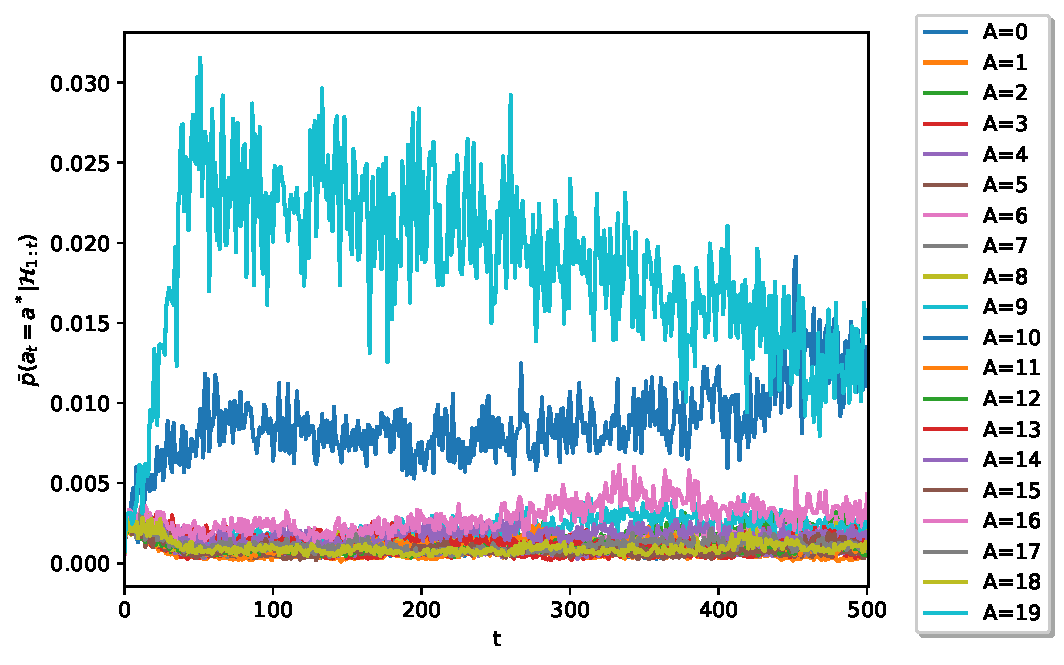
\includegraphics[width=0.85\textwidth]{./fods_figs/yahoo/yahoo_logistic_dynamic}
	\vspace*{-2ex}
	\caption{Empirical probability of playing each bandit arm over time, for SMC-based dynamic logistic Thompson sampling.
		The proposed dynamic bandit policy captures the changing popularity of articles over time.}
	\label{fig:yahoo_logistic_dynamic}
\end{figure}

% Table
\input{table_yahoo_logistic}


\section{Conclusion}
\label{sec:conclusion}

We contribute to the field of sequential decision processes by proposing a Bayesian nonparametric mixture model based Thompson sampling.
We merge advances in the field of Bayesian nonparametrics with a state-of-the art MAB policy (\ie Thompson sampling), allowing for its extension to complex multi-armed bandit domains where there is model uncertainty.

The proposed algorithm provides flexible modeling of convoluted reward functions with convergence guarantees, and attains the exploration-exploitation trade-off in complex MABs with minimal assumptions.

We provide an asymptotic upper bound for the expected cumulative regret of the proposed Dirichlet process Gaussian mixture model based Thompson sampling.

In addition, empirical results show improved cumulative regret performance of the proposed nonparametric Thompson sampling in challenging domains ---where there is model uncertainty--- remarkably adjusting to the complexity of the underlying bandit in an online fashion ---bypassing model mispecification and hyperparameter tuning.

Important savings are attained for complex bandit settings (\eg unbalanced and heavy tailed reward distributions, and bandits with different per-arm reward distributions), where alternative methods struggle.

The competitive advantage lies on the capacity of Bayesian nonparametrics to adjust the complexity of the posterior density to the sequentially observed bandit data.
With the ability to sequentially learn the Bayesian nonparametric mixture model that best approximates the true reward distribution ---not necessarily in the exponential family--- the proposed method can be applied to diverse MAB settings without stringent model specifications and attain reduced regret.

A future direction is to tighten the presented regret bound, as well as to apply the proposed method to real-life MAB applications where complex models are likely to outperform simpler ones.

% BibTeX users please use one of
%\bibliography{../literature}   % name your BibTeX data base
% Select a .bst file for the style
\bibliographystyle{abbrvnat}
% For submission, need to paste the .bbl content here
\documentclass{article}
\usepackage[margin=1.5in]{geometry}

% insert here the call for the packages your document requires
%\usepackage{latexsym}
% Formatting
\usepackage{hyperref}       % hyperlinks
\usepackage{url}            % simple URL typesetting
\usepackage{enumitem}
\usepackage{ifthen}
\usepackage{sidecap}
\usepackage{helvet}
\usepackage{afterpage}
% Package added for words that contain a dash use \-/
\usepackage[shortcuts]{extdash}
\usepackage[htt]{hyphenat}
% Math
\usepackage{amsmath}
\usepackage{amsfonts}	% blackboard math symbols
\usepackage{mathtools}	% For \coloneq
\usepackage{nicefrac}       % compact symbols for 1/2, etc.
\usepackage{microtype}      % microtypography
\usepackage{dsfont} % Indicator that works with Type1

% Graphics
\usepackage{graphicx}
\usepackage{caption}
\usepackage{subcaption}
\usepackage{wrapfig}
\usepackage{float} %Stay where told

% Tables
\usepackage{booktabs}       % professional-quality tables
\usepackage{multirow} % to be able to have multiple row expanding cell
\usepackage[table]{xcolor}
\usepackage{arydshln} % For hdashline% New column types, left/center/right text aligned, given horizontal width
\usepackage{ragged2e} % To justify table text
\newcolumntype{L}[1]{>{\raggedright\let\newline\\\arraybackslash\hspace{0pt}}m{#1}}
\newcolumntype{C}[1]{>{\centering\let\newline\\\arraybackslash\hspace{0pt}}m{#1}}
% For some reason, justify seems to add some vertical space, remove with vspace
\newcolumntype{J}[1]{>{\vspace*{-2ex}\justify\let\newline\\\arraybackslash\hspace{0pt}}m{#1}}
\newcolumntype{R}[1]{>{\raggedleft\let\newline\\\arraybackslash\hspace{0pt}}m{#1}}

% Algorithms
\usepackage{algorithm}
\usepackage{algorithmic}
% Theorems/lemmas
\usepackage{amsthm}
\newtheorem{theorem}{Theorem}[section]
\newtheorem{corollary}{Corollary}[theorem]
\newtheorem{lemma}[theorem]{Lemma}

% To draw graphs (load after xcolor to avoid options clash)
\usepackage{tikz}
\usetikzlibrary{bayesnet} % Library for bayesian networks

% Bibliography
\usepackage{natbib}
% To be able to have references in 2 columns with equal length
\usepackage{flushend}
% etc.
%
% please place your own definitions here and don't use \def but \newcommand{}{}
%%%% iurteaga definitions and macros
% Dolor definitions
%\def\bluecolor#1{\textcolor[rgb]{0,0,1}{\bf #1}}
%\def\greencolor#1{\textcolor[rgb]{0,1,0}{\bf #1}}
%\def\redcolor#1{\textcolor[rgb]{1,0,0}{\bf #1}}

% TODO
\newcommand{\TODO}[1]{\textcolor{red}{TODO: #1}}

% Abbreviations
\newcommand{\iid}{i.i.d. }
\newcommand{\ie}{i.e., }
\newcommand{\Ie}{I.e., }
\newcommand{\eg}{e.g., }
\newcommand{\Eg}{E.g., }
\newcommand{\etAl}{et al.\xspace}

% Real line
\newcommand{\Real}{{\mathbb R}} 
% Natural numbers
\newcommand{\Natural}{{\mathbb N}} 

% Probability related
\newcommand{\Prob}[1]{\mathbb{P}\left( #1 \right)}
% with 2 arguments, for probability model in subscript
\newcommand{\myProb}[2]{\mathbb{P}_{#1}\left( #2 \right)}
%Expected value
\newcommand{\eValue}[2]{\mathbb{E}_{#1}\left\{ #2 \right\}}
\newcommand{\Var}[1]{\mathbb{V}\mathrm{ar} \left\{ #1 \right\}}
\newcommand{\indep}{{\;\bot\!\!\!\!\!\!\bot\;}}
% Kullback-Leibler
\newcommand{\KL}[2]{\mathrm{KL}\left( #1 \| #2\right)}
% Distributions
\newcommand{\N}[1]{\mathcal{N}\left( #1\right)}
\newcommand{\MN}[1]{\mathcal{MN}\left( #1\right)}
\newcommand{\T}[1]{\mathcal{T}\left( #1\right)}
\newcommand{\MT}[1]{\mathcal{MT}\left( #1\right)}
\newcommand{\Dir}[1]{\mathcal{Dir}\left( #1\right)}
\newcommand{\Mult}[1]{{\rm Mult}\left( #1\right)}
\newcommand{\Cat}[1]{{\rm Cat}\left( #1\right)}
\newcommand{\Bin}[1]{{\rm Bin}\left( #1\right)}
\newcommand{\IG}[1]{\mathcal{IG}\left( #1\right)}
\newcommand{\NIG}[1]{\mathcal{NIG}\left( #1\right)}
\newcommand{\NIX}[1]{\mathcal{NIX}\left( #1\right)}
\newcommand{\IW}[1]{\mathcal{IW}\left( #1\right)}
\newcommand{\NIW}[1]{\mathcal{NIW}\left( #1\right)}
\newcommand{\Beta}[1]{\mathcal{Beta}\left( #1\right)}
\newcommand{\Ber}[1]{{\rm Ber}\left( #1\right)}
\newcommand{\U}[1]{\mathcal{U}\left( #1\right)}

% My small matrix
\newcommand{\mySmallMatrix}[1]{\left(\begin{smallmatrix} #1 \end{smallmatrix}\right)}
%Determinant
\newcommand{\mydet}[1]{\left| #1 \right|}
\newcommand{\tr}[1]{\mathrm{tr}\left\{ #1 \right\}} % trace
\newcommand{\diag}{\mathrm{diag}}
% My indicator function
\newcommand{\myind}[1]{\mathds{1}\left[#1\right]}
% d in integral
\newcommand{\dd}[1]{\mathrm{d} #1}

% Useful in Bandits
\newcommand{\A}{\mathcal{A}}
\newcommand{\Astar}{A^*}
\newcommand{\astar}{a^*}
\newcommand{\pstar}{p^*}
\newcommand{\pistar}{\pi^*}
\newcommand{\Atilde}{\tilde{A}}
\newcommand{\atilde}{\tilde{a}}
\newcommand{\ptilde}{\tilde{p}}
\newcommand{\pitilde}{\tilde{\pi}}
\newcommand{\thetastar}{\theta^*}
\newcommand{\thetatilde}{\tilde{\theta}}
\newcommand{\Y}{\mathcal{Y}}
\newcommand{\HH}{\mathcal{H}}

\newcommand{\myPi}[2]{\pi_{#1}\left( #2 \right)}
%\newcommand{\myPistar}[1]{\pi_{p^*}^*\left( #1 \right)}
\newcommand{\myPistar}[1]{\pi_{p^*}\left( #1 \right)}
%\newcommand{\myPitilde}[1]{\tilde{\pi}_{\ptilde}\left( #1 \right)}
\newcommand{\myPitilde}[1]{\pi_{\ptilde}\left( #1 \right)}

%Others
\newcommand{\eqd}{\stackrel{d}{=}} % equal in distribution/law/measure
\newcommand{\deq}{:=} % Define equality
\newcommand{\abs}[1]{|{#1}|}
\newcommand{\argmax}{\mathop{\mathrm{argmax}}}
\newcommand{\argmin}{\mathop{\mathrm{argmin}}}
\newcommand{\eps}{\varepsilon}
%%%%%%%% end iurteaga %%%%%%%% 

%%%%%%%% end iurteaga %%%%%%%% 

\title{Nonparametric Gaussian Mixture Models \\ for the Multi-Armed Contextual Bandit}

\author{ I\~{n}igo Urteaga and Chris H.~Wiggins\\
	{\sf \{inigo.urteaga, chris.wiggins\}@columbia.edu} \\\\
	Department of	Applied Physics and Applied Mathematics\\
	Data Science Institute\\
	Columbia University\\
	New York City, NY 10027
}

\begin{document}
	
\maketitle

\begin{abstract}
We here adopt Bayesian nonparametric mixture models to extend multi-armed bandits in general, and Thompson sampling in particular, to scenarios where there is reward model uncertainty. In the stochastic multi-armed bandit, where an agent must learn a policy that maximizes long term payoff, the reward for the selected action is generated from an unknown distribution. Thompson sampling is a generative and interpretable multi-armed bandit algorithm that has been shown both to perform well in practice, and to enjoy optimality properties for certain reward functions. Nevertheless, Thompson sampling requires knowledge of the true reward model, for calculation of expected rewards and sampling from its parameter posterior. In this work, we extend Thompson sampling to complex scenarios where there is model uncertainty, by adopting a very flexible set of reward distributions: Bayesian nonparametric Gaussian mixture models. The generative process of Bayesian nonparametric mixtures naturally aligns with the Bayesian modeling of multi-armed bandits: the nonparametric model autonomously determines its complexity as new rewards are observed for the played arms. By characterizing each arm's reward distribution with independent nonparametric mixture models, the proposed method sequentially learns the model that best approximates the true underlying reward distribution, achieving successful performance in complex ---not in the exponential family--- bandits. Our contribution is valuable for practical scenarios, as it avoids stringent case-by-case model specifications and hyperparameter tuning, yet attains reduced regret in diverse bandit settings.
\end{abstract}

\section{Introduction}
\label{sec:intro}
% !TEX root = main.tex
Sequential decision making aims to optimize interactions with the world (exploit), while simultaneously learning how the world operates (explore). The origins of the study of the exploration-exploitation trade-off can be traced back to the beginning of the past century, with important contributions within the field of statistics by~\citet{j-Thompson1935} and later~\citet{j-Robbins1952}.
The multi-armed bandit (MAB) is a natural abstraction for a wide variety of real-world challenges that require learning while simultaneously maximizing rewards~\citep{b-Lattimore2020}. The name `bandit' finds its origin in the playing strategy one must devise when facing a row of slot machines~\citep{j-Lai1985}. The contextual MAB, where at each interaction with the world side information (known as `context') is available, is a natural extension of the bandit problem. Recently, a renaissance of the study of MAB algorithms has flourished~\citep{ip-Agrawal2012,ip-Maillard2011}, attracting interest from industry as well, due to its impact in digital advertising and products~\citep{ip-Li2010}. 

\citet{j-Thompson1933} sampling %, also known as posterior sampling~\cite{j-Russo2014}, 
provides an elegant approach that tackles the exploration-exploitation dilemma in MABs. It updates a posterior over expected rewards for each arm, and chooses actions based on the probability that they are optimal. It has been empirically and theoretically proven to perform competitively for MAB models within the exponential family~\citep{ip-Agrawal2013a,ip-Agrawal2013,ic-Korda2013}. Its applicability to the more general reinforcement learning setting of Markov decision processes~\citep{j-Burnetas1997} has recently tracked momentum as well~\citep{ip-Gopalan2015,ic-Ouyang2017}.

Thompson sampling, and the Bayesian approach to the MAB problem, facilitate not only generative and interpretable modeling, but sequential and batch processing as well.
A Thompson sampling policy requires access to posterior samples of the model.
Unfortunately, maintaining such posterior is intractable for distributions not in the exponential family~\citep{j-Russo2018}.
Therefore, developing practical MAB methods to balance exploration and exploitation in real-life domains that might not pertain to such reward family remains largely unsolved.

In an effort to extend Thompson sampling to more complex scenarios, researchers have considered other flexible reward functions and Bayesian inference.
Recent approaches have embraced Bayesian neural networks and approximate inference for Thompson sampling. Variational methods, stochastic mini-batches, and Monte Carlo techniques have been studied for uncertainty estimation of reward posteriors~\citep{ip-Blundell2015, ic-Kingma2015, ip-Lipton2018, ic-Osband2016, ip-Li2016}.

~\citet{ip-Riquelme2018} have benchmarked such techniques and reported that neural networks with approximate inference, even if successful for supervised learning, under-perform in the MAB setting. In particular, they emphasize the issue of adapting the slow convergence uncertainty estimates of neural network based methods to MABs.
In parallel, others have focused on extending Thompson sampling by targeting alternative classes of reward functions, such as approximating the unknown bandit reward functions with Gaussian mixture models~\citep{ip-Urteaga2018}; or maintaining and incrementally updating an ensemble of plausible models that approximates the (otherwise intractable) posterior distribution of interest~\citep{ip-Lu2017}.

An alternative view of Thompson sampling relies on the notion that posterior sampling can be viewed as a perturbation scheme that is sufficiently optimistic.
This point was noted by~\citet{ip-Agrawal2013, ip-Agrawal2013a}, and several authors have analyzed how estimating the bandit reward means with a follow-the-perturbed-leader exploration approach can be successful in the bandit setting.
Bootstrapping techniques that use a combination of observed and artificially generated data have been introduced for the multi-armed bandit and reinforcement learning problems by~\citet{j-Osband2015,j-Eckles2019}.
Bootstrapping over artificial data induces a prior distribution that is critical for effective exploration.
Recently, pseudo-rewards based bootstrapping has also been studied for the multi-armed bandit setting~\citep{ip-Kveton2019,ip-Kveton2019a}, where the pseudo-rewards are used to increase the variance of the bootstrap mean, leading to exploration.~\citet{ip-Kveton2019} show how these pseudo-rewards introduce bias that has to be controlled, which their proposed algorithm achieves, resulting in sublinear regret for Bernoulli bandits.
%A similar perturbed-history exploration based algorithm for the safe online learning to re-rank problem is introduced in~\cite{ip-Li2020}.

In our work, we explore a different route, in which instead of following the perturbation scheme view of posterior sampling, we focus on the Bayesian generative modeling view of Thompson sampling. Even if, for bandit regret minimization, proper modeling of the full reward distributions may not be in general necessary, we defend that a statistical modeling-based approach, which leverages the advances on nonparametric density estimation within statistics, can be performant in the multi-armed bandit setting.

We argue that modeling bandit reward distributions via nonparametric Bayesian mixtures, which adjust to the complexity of the underlying reward model, can provide successful bandit performance. 
Our contribution is on exploiting Bayesian nonparametric mixture models for Thompson sampling to perform MAB optimization. 
To that end, we propose to combine Thompson Sampling with nonparametric Bayesian mixture models that can accommodate continuous reward functions, and develop a Thompson sampling algorithm that ---without incurring on model misspecification--- adapts to a wide variety of complex bandits.

Bayesian nonparametrics have been considered for MAB problems to accommodate continuous actions via Gaussian processes (GPs)~\citep{ip-Srinivas2010,ip-Gruenewaelder2010,ic-Krause2011}, or to allow for an unknown yet countable number of actions via hierarchical Pitman-Yor processes~\citep{j-Battiston2018}.
GPs are powerful nonparametric methods for modeling distributions over continuous functions~\citep{b-Rasmussen2005}, and have been used to model a continuum of MAB actions~\citep{ic-Krause2011}.
Exact inference with GPs is computationally demanding ---it scales cubically in the number of observations--- limiting their applicability to the online setting, even if advancements such as pseudo-observations~\citep{ic-Snelson2006} or variational inference~\citep{ip-Titsias2009} can mitigate these shortcomings. 
Alternatively, \citet{j-Battiston2018} consider MABs with a discrete but unknown action space, and propose a hierarchical Pitman-Yor process for the unknown populations, with per-arm Bernoulli reward distributions. In this work, we are not interested in a nonparametric prior over arms (with specific per-arm reward distributions), but in MABs with a discrete set of actions, for which there is uncertainty on the per-arm reward model.

We propose to account for reward model uncertainty by combining the flexibility of Bayesian nonparametrics with the large hypothesis space of mixture models. In many contexts, a countably infinite mixture is a very realistic model to assume, and has been shown to succeed in modeling a diversity of phenomena~\citep{j-Gershman2012}. Nonparametric processes are useful priors for Bayesian density estimation. Within such framework, one uses nonparametric prior distributions over the mixing proportions, such as Dirichlet or Pitman-Yor processes~\citep{j-Teh2010}.

These models do not only avoid explicitly specifying the number of mixtures, but allow for an unbounded number of mixtures to appear as data are observed. The important issue of nonparametric posterior consistency, with convergence guarantees for a wide class of mixture models, has already been settled~\citep{j-Ghosal1999, j-Ghosal2001, j-Lijoi2004, j-Ghosal2007}.

We here model each of the MAB arm reward functions with per-arm nonparametric mixture models, \ie the complex unknown mapping of the observed per-arm rewards is estimated with nonparametric Gaussian mixture models. By means of a Bayesian nonparametric model, we can accurately approximate continuous reward distributions, yet have analytically tractable inference and online update rules, which allow for sequential adjustment of the complexity of the model to the observed data.
For learning such a nonparametric distribution within the MAB setting, we leverage the well-established advances in Markov chain Monte Carlo methods for Bayesian nonparametric models~\citep{j-Neal2000}.

It is both the combination of nonparametric Bayesian mixture models with Thompson sampling (\ie merging statistical advances with a state-of-the art bandit algorithm), as well as the resulting flexibility and generality (\ie avoiding model misspecification) that is novel in this work.
We note that the generative interpretation of Bayesian nonparametric processes aligns well with the sequential nature of the MAB problem.
To the best of our knowledge, no other work uses Bayesian nonparametric mixtures to model per-arm reward functions in contextual MABs.

Our specific contributions are:
\begin{enumerate}
	\item To propose a unique, yet flexible Thompson sampling-based bandit method that learns the Bayesian nonparametric mixture model that best approximates the true, but unknown, underlying reward distribution per-arm, adjusting its complexity as it sequentially observes data.
	
	\item An asymptotic regret bound for the proposed Thompson sampling algorithm, which assumes a Dirichlet process Gaussian mixture model prior, of order $O(|\A| \log^\kappa T \sqrt{T})$; where $|\A|$ denotes the number of bandit arms, $T$ the number of agent iterations with the environment, and the constant $\kappa\geq 0$ depends on the tail behavior of the true reward distribution and the priors of the Dirichlet process.
	
	\item To demonstrate empirically that the proposed nonparametric Thompson sampling method: 
	\begin{enumerate}
		\item attains reduced regret in complex MABs ---with different unknown per-arm distributions not in the exponential family--- when compared to state-of-the art baseline bandit algorithms; and
		\item is as good as an Oracle (i.e., one that knows the true underlying model class) that implements a Thompson sampling policy, \ie the proposed per-arm nonparametric posterior densities quickly converge to the true unknown distributions, incurring in minimal additional bandit regret.
	\end{enumerate}	
\end{enumerate}

These contributions are valuable for bandit scenarios in the presence of model uncertainty, \ie in real-life.
The same algorithm ---which automatically adjusts its complexity to the observed bandit data--- is run for complex (not in the exponential family) multi-armed bandits.
The proposed Thompson sampling method avoids hyperparameter tuning and case-by-case reward model design choices (bypassing model mispecification) yet attains reduced regret.

\section{Background}
\label{sec:background}
% !TEX root = smc_bandits.tex
\subsection{Multi-armed bandits}
\label{ssec:mab}
\input{mab}

\subsection{Sequential Monte Carlo}
\label{ssec:smc}
\input{smc}

\section{Bayesian nonparametric Thompson sampling}
\label{sec:proposed_method}
% !TEX root = main.tex
We combine Bayesian nonparametric mixture models with Thompson sampling for MABs under model uncertainty. We consider an independent set of nonparametric mixture models $G_{a}$ per-arm (with their own hyperparameters $d_a$,$\gamma_a$, and base measure $G_{a,0}$) allowing for flexible, potentially different, reward distributions for each arm $a\in\A$ of the MAB.
The graphical model of the Bayesian nonparametric bandit is rendered in Figure~\ref{fig:pgm_nonparametric_bandit}, where we assume complete independence of each arm's reward distribution.\footnote{An alternative model would be to consider a hierarchical nonparametric model~\citep{j-Teh2006,j-Teh2010}, where all arms are assumed to obey the same family of distributions, but only their mixture proportions vary across arms. We provide details of this alternative model in Section~\ref{asec:nonparametric_hierarchical_mixture_model} of the Appendix.}

% Nonparametric bandit graphical model
\begin{figure}[!h]
	\begin{center}
			\input{nonparametric_mixture_bandit_pgm_indep_horizontal}
		\caption{The Bayesian nonparametric mixture bandit, as a probabilistic graphical model.}
		\label{fig:pgm_nonparametric_bandit}
		\vspace*{-4ex}
	\end{center}
\end{figure}

By characterizing each arm of the bandit with a different nonparametric model, we enjoy full flexibility to estimate each per-arm distribution independently, covering MAB cases with distinct reward model classes per-arm. This setting is a very powerful extension of the MAB problem, which has not attracted interest so far, yet can circumvent model misspecification.

At every interaction of the MAB agent with the environment, reward $y_{t,a_t}$ is \iid drawn from a context dependent unknown distribution $Y_{t,a_t}\sim p(Y|a_t,x_t,\thetastar)$ of the played arm $a_t$, which we here approximate via Bayesian nonparametric mixture models~\citep{b-Ghosal2017}.

Specifically, we model context-conditional reward densities with nonparametric Gaussian mixtures per-arm, \ie
\begin{align}
Y_{t,a} \sim p(Y|a,x_t,\varphi_a) &= \sum_{k=1}^{K_a} \frac{n_{a,k}-d_a}{n_a+\gamma_a} \cdot \N{Y|x_{t}^\top w_{a,k}, \sigma_{a,k}^2} \nonumber \\
& \qquad + \frac{\gamma_a+K_ad_a}{n_a+\gamma_a} \N{Y|x_{t}^\top w_{a,k_{new}}, \sigma_{a,k_{new}}^2} \;,
\label{eq:nonparametric_Gaussian_mixture}
\end{align}
where the number of mixands $K_a$ is determined by independent per-arm Pitman-Yor processes: $n_{a,k}$ refers to the rewards observed after playing arm $a$ that are assigned to mixture $k$, and $n_a=\sum_{k=1}^{K_a}n_{a,k}$.
After $n_{a}$ observations for arm $a$, there are $K_a$ already `\textit{seen}' mixtures, and a probability of $\frac{\gamma_a+K_ad_a}{n_a+\gamma_a}$ of incorporating a new mixand $k_{new}$ to the mixture.

Eqn.~\eqref{eq:nonparametric_Gaussian_mixture} describes per-arm nonparametric Gaussian mixture densities, with a Pitman-Yor nonparametric prior as described in Eqn.~\eqref{eq:pitman_yor_mixture}.
Each per-arm distribution is modeled independently with per-arm specific parameterizations: $d_a$, $\gamma_a$, $\varphi_{a,k}=\{w_{a,k}, \sigma_{a,k}^2 \}$, for $k={1,\cdots, K_a}$. 

The proposed contextual nonparametric model relies on leveraging context-conditional Gaussian models (with an expected value that is linearly dependent on the context at time $t$, \ie $\mu_{t,a,k}=x_t^\top w_{a,k}$), and extending them to a potentially infinite mixture.
As the number of mixands $K_a$ grows, the nonparametric distribution can be non-linear in the context.

With the proposed per-arm nonparametric mixture of Gaussian densities, we make a very flexible reward model assumption that automatically adjusts to the observed data: we are nonparametrically estimating complex, unknown per-arm continuous reward densities.
We leverage the well known linear Gaussian model and allow for the nonparametric model to accommodate as many mixands as necessary to best describe the observed bandit data.

The proposed Bayesian nonparametric model provides a flexible approach to density estimation, which can arbitrarily approximate continuous distributions. 
The Bayesian nonparametric literature has already established strong convergence results on the density estimation properties of these models: for a wide class of continuous distributions, the nonparametric posterior converges to the true data-generating density, under mild regularity conditions~\citep{j-Ghosal1999, j-Lijoi2004, j-Tokdar2006, j-Ghosal2007, j-Bhattacharya2010, j-Pati2013}.

In theory, the proposed Bayesian nonparametric model is on an infinite-dimensional parameter space (\ie the Pitman-Yor process can accommodate countably infinite mixands).
In practice, the model as in Eqn.~\eqref{eq:nonparametric_Gaussian_mixture} will use a finite subset of the available parameter dimensions to explain a finite sample of observations: \ie it sets the number of mixands per-arm $K_a$ according to the observed per-arm rewards.
Consequently, the effective complexity of the resulting model (\ie the dimensionality $K_a$ in Eqn.~\eqref{eq:nonparametric_Gaussian_mixture}) adapts to the observed data.

\subsection{Nonparametric context-conditional Gaussian mixture model posterior}
\label{ssec:nonparametric_posterior_update}

We now derive the procedure for inference of the per-arm, context-dependent reward posterior density of the proposed Bayesian nonparametric Gaussian mixture model.
As outlined in Section~\ref{ssec:background_nonparametric_mixture_model}, we rely on auxiliary latent variables per-arm $z_{1:n_a}$, and implement a Gibbs sampler that iterates between sampling mixture assignments $z_{1:n_a}$, and updating the emission distribution parameter posterior $G_{n_{a,k}}(\varphi_{a,k})$ for each arm and mixture. 

We start with the derivation of the parameter posteriors.
Per-arm and per-mixand emission distributions in Eqn.~\eqref{eq:nonparametric_Gaussian_mixture} are context-conditional Gaussian densities
\begin{equation}
\N{Y|x^\top w_{a,k}, \sigma_{a,k}^2} \; ,
\end{equation}
where $x^\top w_{a,k}$ and $\sigma_{a,k}^2$ are the means and variances, respectively, of the $k$-th mixand of arm $a$ in round $t$.
The conjugate prior of each of the mixands is a Normal-inverse Gamma,
\begin{equation}
G_{a,0}(\varphi_a) = \NIG{w_a, \sigma_a^2 |U_{a,0}, V_{a,0},\alpha_{a,0}, \beta_{a,0}} \;, 
\end{equation}
with hyperparameters $\varPhi_{a,0}=\{U_{a,0}, V_{a,0},\alpha_{a,0}, \beta_{a,0}\}$.

After observing rewards $y_{1:n}$, and conditioned on the auxiliary assignment variables $z_{1:n_a}$, the posteriors of per-arm and mixand parameters $\varphi_{a,k}$ follow a Normal-inverse Gamma distribution with updated hyperparameters $\varPhi_{a,k,n_{a,k}}$:
\begin{align}
G_{a,n_{a,k}}(\varphi_{a,k}) &=\NIG{w_{a,k}, \sigma_{a,k}^2 |\varPhi_{a,k,n_{a,k}}} \;, \\
\varPhi_{a,k,n_{a,k}}& =\{U_{a,k,n_{a,k}}, V_{a,k,n_{a,k}},\alpha_{a,k,n_{a,k}}, \beta_{a,k,n_{a,k}} \} \;, \nonumber
\end{align}
that depend on the number $n_{a,k}$ of rewards observed after playing arm $a$ that are assigned to mixand $k$. Specifically,
\begin{equation}
\begin{cases}
V_{a,k,n_{a,k}}^{-1} = x_{1:n} R_{a,k} x_{1:n}^\top + V_{a,0}^{-1} \;,\\
U_{a,k,n_{a,k}}= V_{a,k,n_{a,k}} \left( x_{1:n} R_{a,k} y_{1:n} + V_{a,0}^{-1} U_{a,0}\right) \;, \\
\alpha_{a,k,n_{a,k}} = \alpha_{a,0} + \frac{1}{2} \tr{R_{a,k}} \;, \\
\beta_{a,k,n_{a,k}} = \beta_{a,0} + \frac{1}{2}\left(y_{1:n}^\top R_{a,k}y_{1:n} \right) + \frac{1}{2}\left( U_{a,0}^\top V_{a,0}^{-1} U_{a,0} - U_{a,k,n_{a,k}}^\top V_{a,k,n_{a,k}}^{-1} U_{a,k,n_{a,k}} \right) \; ,
\end{cases}
\label{eq:posterior_hyperparameters}
\end{equation}
where $R_{a,k}\in\Real^{n_a\times n_a}$ is a sparse diagonal matrix with elements $\left[R_{a,k}\right]_{i,i}=\mathds{1}[a_i=a,z_i=k]$ for $i=\{0,\cdots, n_a\}$, and $n_{a}=\sum_{k=1}^{K_a} n_{a,k}$ is the number of rewards observed after playing arm $a$. The number of mixands per-arm $K_a$ of the bandit is independently drawn from its own Pitman-Yor process. Note that the above expression can be computed sequentially as data are observed for the played arm.

The predictive emission distribution after marginalization of the parameters $\varphi_{a,k}$, needed for solving Eqn.~\eqref{eq:gibbs_mixture_assignment}, follows a conditional Student-t distribution
\begin{align}
p_{a,k}(Y|a,x,\varPhi_{a,k,,n_{a,k}}) &= \T{Y|\nu_{a,k,n_{a,k}}, m_{a,k,n_{a,k}}, r_{a,k,n_{a,k}}} \;, \nonumber \\
\text{with } \varPhi_{a,k,,n_{a,k}} &=
\begin{cases}
\nu_{a,k,n_{a,k}}=2\alpha_{a,k} \;, \\
m_{a,k,n_{a,k}} = x^\top U_{a,k} \;, \\
r_{a,k,n_{a,k}}^2 = \frac{\beta_{a,k}}{\alpha_{a,k}} (1+x^\top V_{a,k} x) \;.
\end{cases}
\label{eq:marginalized_predictive_emission_univariate}
\end{align}
The hyperparameters $\varPhi_{a,k,,n_{a,k}}=\{\nu_{a,k,n_{a,k}}, m_{a,k,n_{a,k}}, r_{a,k,n_{a,k}}\}$ above are those of the prior $\varPhi_{a,0}$, or the posterior $\varPhi_{a,k,n_{a,k}}$, depending on whether the predictive density refers to a `\textit{new}' mixand $k_{new}$ with $n_{a,k=k_{new}}=0$, or a `\textit{seen}' mixand $k$, for which $n_{a,k}\geq0$ observations have been already assigned to, respectively.

Similarly, the likelihood of a set of rewards assigned to per-arm mixand $k$, $Y_{a,k}=y_{1:n}\cdot \mathds{1}[a_n=a,z_n=k]$, given their associated contexts $X_{a,k}=x_{1:n} \cdot \mathds{1}[a_n=a,z_n=k]$, follows the matrix t-distribution
\begin{align}
&p(Y_{a,k}|X_{a,k},X_{\backslash a,k},Y_{\backslash a,k},\varPhi_{a,k}) = \MT{Y_{a,k}|\nu_{Y_{a,k}}, M_{Y_{a,k}}, \Psi_{Y_{a,k}}, \Omega_{Y_{a,k}}} \; , \nonumber  \\
\text{with }&\begin{cases}
\nu_{Y_{a,k}}=2 \alpha_{a,k} \;,\\
M_{Y_{a,k}}= X_{a,k}^\top U_{a,k} \;, \\
\Psi_{Y_{a,k}} = I_{n_{a,k}} + X_{a,k}^\top V_{a,k} X_{n_{a,k}} \;,\
\Omega_{Y_{a,k}} = 2 \beta_{a,k} \;.
\end{cases}
\label{eq:marginalized_predictive_emission_multivariate}
\end{align}

With parameter posteriors as in Eqns.~\eqref{eq:marginalized_predictive_emission_univariate} and~\eqref{eq:marginalized_predictive_emission_multivariate}, we implement a Gibbs sampler to infer the mixture assignments $z_{1:n}$, based on the assignment probabilities described in Eqn.~\eqref{eq:gibbs_mixture_assignment}, for per-arm already drawn mixture components $k_a\in\{1, \cdots, K_a\}$, and a new `\textit{unseen}' mixand $k_{a,new}$. Therefore, the proposed Gibbs sampler adjusts the nonparametric posterior's complexity (\ie number of mixands $K_a$) according to the observed per-arm rewards distribution.

\subsection{Nonparametric Gaussian mixture model based Thompson sampling}
\label{ssec:nonparametric_thompson_sampling}

We leverage the nonparametric context-conditional Gaussian mixture model described above, and combine it with a posterior sampling MAB policy, \ie Thompson sampling~\citep{j-Russo2018}. The proposed Thompson sampling technique for contextual bandits with nonparametric Gaussian mixture reward models is presented in Algorithm~\ref{alg:nonparametric_ts}.

%Nonparametric TS
\vspace*{-2ex}
\begin{algorithm}
	\caption{Nonparametric Gaussian mixture model based Thompson sampling}
	\label{alg:nonparametric_ts}
	\begin{algorithmic}[1]
		\STATE {\bfseries Input:} Number of arms $|\A|$
		\STATE {\bfseries Input:} Per-arm hyperparameters $d_a$, $\gamma_a$, $\varPhi_{a,0}$
		\STATE {\bfseries Input:} Gibbs convergence criteria $\epsilon$, $Gibbs_{max}$ 
		\STATE $\HH_1=\emptyset$
		\FOR{$t=1, \cdots, T$}
		\STATE Receive context $x_{t}$
		\FOR{$a=1, \cdots, |\A|$}
		\STATE Draw parameters from the posterior \\ $\hspace*{2ex}\varphi_{a,k}^{(t)} \sim G_{a,k,n_{a,k}}(\varPhi_{a,k}), \forall k$, as in Eqn.~\eqref{eq:posterior_hyperparameters}
		\STATE Compute $\mu_{t,a}(x_{t},\varphi_{a}^{(t)})$ as in Eqn.~\eqref{eq:nonparametric_expected_reward}
		\ENDFOR
		\STATE Play arm $a_{t}=\argmax_{a^\prime \in \A} \mu_{t,a^\prime}(x_{t},\varphi_{a^\prime}^{(t)})$
		\STATE Observe reward $y_{t}$
		\STATE $\HH_{1:t}=\HH_{1:t-1} \cup \left\{x_{t}, a_{t}, y_{t}\right\}$
		\WHILE{NOT Gibbs convergence criteria}
		\STATE Update mixture assignments $z_{1:n}$ based on Eqn.~\eqref{eq:gibbs_mixture_assignment}
		\STATE Compute sufficient statistics $n_{a,k}$
		\STATE Update parameter posteriors $\varPhi_{a,k,n_{a,k}}$ based on Eqn.~\eqref{eq:posterior_hyperparameters}
		\ENDWHILE
		\ENDFOR
	\end{algorithmic}
\end{algorithm}
\vspace*{-2ex}

At each interaction with the world, the proposed Thompson sampling decides which arm to play next based on a random parameter sample, drawn from the posterior nonparametric distribution updated with all the information available at time $t$.

The parameters' posterior distributions for the proposed nonparametric Gaussian mixture model are presented in Section~\ref{ssec:nonparametric_posterior_update}.
Specifically, for nonparametric models as in Eqn~\eqref{eq:nonparametric_Gaussian_mixture}, one draws per-arm and per-mixand Gaussian parameters $\varphi_{a,k}$ from the posterior distributions with updated hyperparameters $\varPhi_{a,k,n_{a,k}}$ in Eqn.~\eqref{eq:posterior_hyperparameters}, conditioned on the mixture assignments $z_{1:n}$ determined by the Gibbs sampler in Eqn.~\eqref{eq:gibbs_mixture_assignment}, with marginalized emission densities provided in Eqns.~\eqref{eq:marginalized_predictive_emission_univariate} and~\eqref{eq:marginalized_predictive_emission_multivariate}.

Given the inferred sufficient statistics of the assignments (\ie the counts $n_{a,k}$ of rewards observed for arm $a$ and assigned to mixand $k$), and the drawn posterior parameter samples $w_{a,k}^{(t)}$, one computes the expected reward for each arm of the nonparametric bandit, \ie

\begin{align}
\mu_{t,a}(x_{t},\varphi_{a}^{(t)})&=\sum_{k=1}^{K_a} \frac{n_{a,k}-d_a}{n_a+\gamma_a} \left(x_{t}^\top w_{a,k}^{(t)}\right) + \frac{\gamma_a+K_ad_a}{n_a+\gamma_a} \left(x_{t}^\top w_{a,k_{new}}^{(t)} \right)\; .
\label{eq:nonparametric_expected_reward}
\end{align}

The proposed Thompson sampling policy $\myPitilde{\Atilde_t|x_{t},\HH_{1:t-1}}$, with assumed per-arm nonparametric distribution $\ptilde(Y|a,x_t,\varphi_a)$ in Eqn~\eqref{eq:nonparametric_Gaussian_mixture}, picks the arm that maximizes the above expected reward, \ie
\begin{align}
\myPitilde{\Atilde_t|x_{t},\HH_{1:t-1}}&=\myPitilde{\Atilde_t|x_{t},\varphi_{a}^{(t)}} \nonumber \\
& =\myind{\Atilde_t=\argmax_{a^\prime \in \A} \mu_{t,a}\left(x_{t},\varphi_{a}^{(t)}\right)}\;, \varphi_{a}^{(t)} \sim p(\varphi_{a}|\HH_{1:t-1}) \;,
\end{align}
with updated hyperparameters for $\ptilde(\varphi_{a}|\HH_{1:t-1})$ as in Eqn.~\eqref{eq:posterior_hyperparameters}.

\subsubsection{Regret bound}
\label{sssec:nonparametric_thompson_sampling_regret_bound}

We leverage asymptotic posterior converge rates ---the rate at which the distance between two densities becomes small as the number of observation grows--- to asymptotically bound the regret of the proposed nonparametric Thompson sampling algorithm.

A Thompson sampling-based policy operates according to the probability of each arm being optimal. This probability is equivalent to the expectation with respect to the joint posterior distribution of the expected rewards given history and context, $p(\mu_t|x_{t},\HH_{1:t-1})$, of the optimal arm indicator function, \ie
\begin{align}
\myPi{p}{A_t|x_{t},\HH_{1:t-1}} &= \myProb{p}{A_t=\argmax_{a^\prime \in \A} \mu_{t,a^\prime}} =\eValue{p}{\myind{A_t=\argmax_{a^\prime \in \A}\mu_{t,a^\prime}}} \;.
\nonumber
\end{align}

Note that the indicator function $\myind{A_t=\argmax_{a^\prime \in \A}\mu_{t,a^\prime}}$ for each arm requires the posterior over all arms $a^\prime \in \A$ as input. That is, the posterior $p(\mu_t|x_{t},\HH_{1:t-1})$ is the joint posterior distribution over the expected rewards of all arms: $\mu_{t}=\{\mu_{t,a}\}, \forall a\in \A$; \ie it is a $|\A|$ dimensional multivariate distribution over all arms of the bandit.

We now present our first lemma, with the proof provided in Section~\ref{asec:nonparametric_thompson_sampling_regret_bound} of the Appendix, which is key to the cumulative regret theorem that follows.
\begin{lemma}
	The difference in action probabilities between two Thompson sampling policies, given the same history and context up to time $t$, is bounded by the total-variation distance $\delta_{TV}(p_t,q_t)$ between the posterior distributions of their expected rewards at time $t$, $p_t=p(\mu_{t}|x_t,\HH_{1:t-1})$ and $q_t=q(\mu_{t}|x_t,\HH_{1:t-1})$, respectively,
	\begin{equation}
	\myPi{p_t}{A_t=a} - \myPi{q_t}{A_t=a} \leq \delta_{TV}(p_t,q_t) \; .
	\nonumber
	\end{equation}
	\label{lemma:total_variation_bounds_diff_policies}
	The \textbf{total variation distance} $\delta_{TV}(p,q)$ between distributions $p$ and $q$ on a sigma-algebra $\mathcal{F}$ of subsets of the sample space $\Omega$ is defined as
	\begin{equation}
	\delta_{TV}(p, q) = \sup_{B \in \mathcal{F}} \left|p(B)-q(B)\right| \; ,
	\end{equation}
	which is properly defined for both discrete and continuous distributions (see details in Section~\ref{asec:nonparametric_thompson_sampling_regret_bound} of the Appendix).
\end{lemma}
We make use of Lemma~\ref{lemma:total_variation_bounds_diff_policies} to asymptotically bound the cumulative regret of the proposed Thompson sampling with Dirichlet process priors (\ie $d_a=0, \forall a$) and Gaussian emission distributions, for bandits with true reward densities that meet certain regularity conditions. 

\begin{theorem}
	The expected cumulative regret at time $T$ of a Dirichlet process Gaussian mixture model based Thompson sampling algorithm is asymptotically bounded by
	\begin{equation}
	R_T	\leq \mathcal{O}\left(|\A| \log^\kappa T \sqrt{T} \right) \; \text{ as } T \rightarrow \infty \; .
	\nonumber
	\end{equation}
	We use big-O notation $\mathcal{O}(\cdot)$ for the asymptotic regret bound, as it bounds from above the growth of the cumulative regret over time for large enough bandit interactions, \ie
	\begin{align}
	\lim_{T\rightarrow \infty} \frac{R_T}{|\A| \log^\kappa T \sqrt{T} } & \leq \mathcal{O}(1)\; .
	\end{align}
	We note that this bound holds both in a frequentist and Bayesian view of expected regret.
	\label{th:regret_bound}
\end{theorem}

The proof of Theorem~\ref{th:regret_bound}, provided in Section~\ref{asec:nonparametric_thompson_sampling_regret_bound} of the Appendix, consists of bounding the regret introduced by two factors: the first, related to the use of Thompson sampling (\ie a policy that does not know the true parameters of the reward distribution, but has knowledge of the true reward model class); and the second, a term that accounts for the convergence of the posterior of a nonparametric model to that of the true data generating distribution.

The logarithmic term $\log^\kappa T$ in the bound appears due to the convergence rate of the nonparametric density estimation, where the exponent $\kappa\geq 0$ depends on the tail behavior of the base measure and the priors of the Dirichlet process ---see Section \ref{asec:nonparametric_thompson_sampling_regret_bound} of the Appendix, and references therein, for details on density convergence and its impact on the exponent $\kappa\geq 0$.

\subsubsection{Computational complexity}
\label{sssec:nonparametric_thompson_sampling_computational_complexity}
The Gibbs sampler in the proposed nonparametric Thompson sampling (lines 14-18 within Algorithm~\ref{alg:nonparametric_ts}) is run $Gibbs_{steps}$ until a stopping criteria is met: either the model likelihood of the sampled chain is stable within an $\epsilon$ likelihood margin between steps, or a maximum number of iterations $Gibbs_{max}$ is reached.

As new rewards $y_{t,a_{t}}$ are acquired, updates to assignments $z_{t^\prime,a_{t}}$ are computed sequentially within the Gibbs sampler for $t^\prime=\{1,\cdots,t | a_{t^\prime}=a_{t}\}$; \ie only the posterior over the last played armed $a_{t}$ is recomputed. Since Eqn.~\eqref{eq:posterior_hyperparameters} can be sequentially computed for each per-arm observation, the computational cost of the Gibbs sampler grows with the number of available observation of the played arm. Therefore, the overall computational cost is upper-bounded by $\mathcal{O}(T \cdot Gibbs_{steps})$ per-interaction with the world, \ie per newly observed reward $y_{t,a_{t}}$.

Due to the sequential acquisition of observations in the bandit setting, and the need to only update the posterior for the played arm, the Gibbs sampler is \textit{warm-started} at each bandit interaction, and good convergence can be achieved in few iterations per observed reward. 
In practice, and because of the \textit{warm-start}, one can limit the number of Gibbs sampler iterations per-bandit interaction to upper-bound the algorithm's complexity to $O(T\cdot Gibbs_{max})$ per interaction, yet achieve satisfactory performance ---empirical evidence of this claim is provided in Section~\ref{sssec:evaluation_mixture_scenarios_baselines}.
Due to the \textit{warm-start}, the Gibbs sampler is run from a good starting point: the per-arm parameter space that describes all but this newly observed reward $y_{t,a_{t}}$.

We emphasize that we propose a Gibbs sampler that runs until convergence, but suggest to limit the number of Gibbs iterations as a practical recommendation with good empirical regret performance, yet upper-bounded $\mathcal{O}(T \cdot Gibbs_{max})$ computational complexity per MAB interaction with the environment.


\section{Evaluation}
\label{sec:evaluation}
% !TEX root = smc_bandits.tex
We empirically evaluate the proposed SMC-based Bayesian MAB framework
in non-stationary bandit scenarios
%\footnote{
%	Results in Appendix~\ref{assec:static_bandits_experiments_analytical}
%	validate the performance of SMC-based policies in stationary bandits.
%	We compare their performance to solutions based on analytically attainable posteriors
%	with Bernoulli and contextual linear Gaussian reward functions~\citep{ip-Kaufmann2012,ip-Garivier2011a,ic-Korda2013,ip-Agrawal2013a},
%	as well as for context-dependent binary rewards modeled with the logistic reward function~\cite{ic-Chapelle2011,j-Scott2015} ---Appendix~\ref{assec:static_bandits_experiments_logistic}.
%	Results showcase satisfactory performance across a wide range of stationary bandit parameterizations and sizes,
%	as SMC-based policies achieve the right exploration-exploitation tradeoff.
%}
with continuous, binary and discrete-categorical reward distributions.

Results in Appendix~\ref{assec:static_bandits_experiments_analytical}
validate the performance of SMC-based policies in stationary bandits.
We compare their performance to solutions based on analytically attainable posteriors
with Bernoulli and contextual linear Gaussian reward functions~\citep{ip-Kaufmann2012,ip-Garivier2011a,ic-Korda2013,ip-Agrawal2013a},
as well as for context-dependent binary rewards modeled with the logistic reward function~\cite{ic-Chapelle2011,j-Scott2015} ---Appendix~\ref{assec:static_bandits_experiments_logistic}.
Results showcase satisfactory performance across a wide range of stationary bandit parameterizations and sizes,
as SMC-based policies achieve the right exploration-exploitation tradeoff.

For results we present below, we simulate different parameterizations of dynamic linear models described in Section~\ref{ssec:linear_mixing_dynamics},
and present results for a variety of MAB environments with reward functions detailed in Sections~\ref{ssec:dynamic_bandits_gaussian},~\ref{ssec:dynamic_bandits_logistic} and~\ref{ssec:dynamic_bandits_categorical}.
Section~\ref{ssec:logged_data_bandits} illustrates
the ability of SMC-based bandit policies
to capture non-stationary trends in personalized news article recommendations.

The main evaluation metric is the cumulative regret of the bandit agent, as defined in Equation~\eqref{eq:mab_cumulative_regret},
with results averaged over 500 realizations.
We present results for SMC-based policies with $M=2000$ samples,
and provide an evaluation of the impact of $M$ in Appendix~\ref{asec:dynamic_bandits}.

\subsection{Non-stationary, linear Gaussian rewards}
\label{ssec:dynamic_bandits_gaussian}
\input{dynamic_bandits_gaussian}

\clearpage
\subsection{Non-stationary, logistic rewards}
\label{ssec:dynamic_bandits_logistic}
\input{dynamic_bandits_logistic}

\clearpage
\subsection{Non-stationary, categorical rewards}
\label{ssec:dynamic_bandits_categorical}
\input{dynamic_bandits_categorical}

%\clearpage
\subsection{Bandits for personalized news article recommendation}
\label{ssec:logged_data_bandits}
\input{bandits_news_recommendation}

\section{Conclusion}
\label{sec:conclusion}

We contribute to the field of sequential decision processes by proposing a Bayesian nonparametric mixture model based Thompson sampling.
We merge advances in the field of Bayesian nonparametrics with a state-of-the art MAB policy (\ie Thompson sampling), allowing for its extension to complex multi-armed bandit domains where there is model uncertainty.

The proposed algorithm provides flexible modeling of convoluted reward functions with convergence guarantees, and attains the exploration-exploitation trade-off in complex MABs with minimal assumptions.

We provide an asymptotic upper bound for the expected cumulative regret of the proposed Dirichlet process Gaussian mixture model based Thompson sampling.

In addition, empirical results show improved cumulative regret performance of the proposed nonparametric Thompson sampling in challenging domains ---where there is model uncertainty--- remarkably adjusting to the complexity of the underlying bandit in an online fashion ---bypassing model mispecification and hyperparameter tuning.

Important savings are attained for complex bandit settings (\eg unbalanced and heavy tailed reward distributions, and bandits with different per-arm reward distributions), where alternative methods struggle.

The competitive advantage lies on the capacity of Bayesian nonparametrics to adjust the complexity of the posterior density to the sequentially observed bandit data.
With the ability to sequentially learn the Bayesian nonparametric mixture model that best approximates the true reward distribution ---not necessarily in the exponential family--- the proposed method can be applied to diverse MAB settings without stringent model specifications and attain reduced regret.

A future direction is to tighten the presented regret bound, as well as to apply the proposed method to real-life MAB applications where complex models are likely to outperform simpler ones.

% BibTeX users please use one of
%\bibliography{../literature}   % name your BibTeX data base
% Select a .bst file for the style
\bibliographystyle{abbrvnat}
% For submission, need to paste the .bbl content here
\documentclass{article}
\usepackage[margin=1.5in]{geometry}

% insert here the call for the packages your document requires
%\usepackage{latexsym}
% Formatting
\usepackage{hyperref}       % hyperlinks
\usepackage{url}            % simple URL typesetting
\usepackage{enumitem}
\usepackage{ifthen}
\usepackage{sidecap}
\usepackage{helvet}
\usepackage{afterpage}
% Package added for words that contain a dash use \-/
\usepackage[shortcuts]{extdash}
\usepackage[htt]{hyphenat}
% Math
\usepackage{amsmath}
\usepackage{amsfonts}	% blackboard math symbols
\usepackage{mathtools}	% For \coloneq
\usepackage{nicefrac}       % compact symbols for 1/2, etc.
\usepackage{microtype}      % microtypography
\usepackage{dsfont} % Indicator that works with Type1

% Graphics
\usepackage{graphicx}
\usepackage{caption}
\usepackage{subcaption}
\usepackage{wrapfig}
\usepackage{float} %Stay where told

% Tables
\usepackage{booktabs}       % professional-quality tables
\usepackage{multirow} % to be able to have multiple row expanding cell
\usepackage[table]{xcolor}
\usepackage{arydshln} % For hdashline% New column types, left/center/right text aligned, given horizontal width
\usepackage{ragged2e} % To justify table text
\newcolumntype{L}[1]{>{\raggedright\let\newline\\\arraybackslash\hspace{0pt}}m{#1}}
\newcolumntype{C}[1]{>{\centering\let\newline\\\arraybackslash\hspace{0pt}}m{#1}}
% For some reason, justify seems to add some vertical space, remove with vspace
\newcolumntype{J}[1]{>{\vspace*{-2ex}\justify\let\newline\\\arraybackslash\hspace{0pt}}m{#1}}
\newcolumntype{R}[1]{>{\raggedleft\let\newline\\\arraybackslash\hspace{0pt}}m{#1}}

% Algorithms
\usepackage{algorithm}
\usepackage{algorithmic}
% Theorems/lemmas
\usepackage{amsthm}
\newtheorem{theorem}{Theorem}[section]
\newtheorem{corollary}{Corollary}[theorem]
\newtheorem{lemma}[theorem]{Lemma}

% To draw graphs (load after xcolor to avoid options clash)
\usepackage{tikz}
\usetikzlibrary{bayesnet} % Library for bayesian networks

% Bibliography
\usepackage{natbib}
% To be able to have references in 2 columns with equal length
\usepackage{flushend}
% etc.
%
% please place your own definitions here and don't use \def but \newcommand{}{}
\input{my_definitions}

%%%%%%%% end iurteaga %%%%%%%% 

\title{Nonparametric Gaussian Mixture Models \\ for the Multi-Armed Contextual Bandit}

\author{ I\~{n}igo Urteaga and Chris H.~Wiggins\\
	{\sf \{inigo.urteaga, chris.wiggins\}@columbia.edu} \\\\
	Department of	Applied Physics and Applied Mathematics\\
	Data Science Institute\\
	Columbia University\\
	New York City, NY 10027
}

\begin{document}
	
\maketitle

\begin{abstract}
We here adopt Bayesian nonparametric mixture models to extend multi-armed bandits in general, and Thompson sampling in particular, to scenarios where there is reward model uncertainty. In the stochastic multi-armed bandit, where an agent must learn a policy that maximizes long term payoff, the reward for the selected action is generated from an unknown distribution. Thompson sampling is a generative and interpretable multi-armed bandit algorithm that has been shown both to perform well in practice, and to enjoy optimality properties for certain reward functions. Nevertheless, Thompson sampling requires knowledge of the true reward model, for calculation of expected rewards and sampling from its parameter posterior. In this work, we extend Thompson sampling to complex scenarios where there is model uncertainty, by adopting a very flexible set of reward distributions: Bayesian nonparametric Gaussian mixture models. The generative process of Bayesian nonparametric mixtures naturally aligns with the Bayesian modeling of multi-armed bandits: the nonparametric model autonomously determines its complexity as new rewards are observed for the played arms. By characterizing each arm's reward distribution with independent nonparametric mixture models, the proposed method sequentially learns the model that best approximates the true underlying reward distribution, achieving successful performance in complex ---not in the exponential family--- bandits. Our contribution is valuable for practical scenarios, as it avoids stringent case-by-case model specifications and hyperparameter tuning, yet attains reduced regret in diverse bandit settings.
\end{abstract}

\section{Introduction}
\label{sec:intro}
\input{introduction}

\section{Background}
\label{sec:background}
\input{background}

\section{Bayesian nonparametric Thompson sampling}
\label{sec:proposed_method}
\input{method}

\section{Evaluation}
\label{sec:evaluation}
\input{evaluation}

\section{Conclusion}
\label{sec:conclusion}

We contribute to the field of sequential decision processes by proposing a Bayesian nonparametric mixture model based Thompson sampling.
We merge advances in the field of Bayesian nonparametrics with a state-of-the art MAB policy (\ie Thompson sampling), allowing for its extension to complex multi-armed bandit domains where there is model uncertainty.

The proposed algorithm provides flexible modeling of convoluted reward functions with convergence guarantees, and attains the exploration-exploitation trade-off in complex MABs with minimal assumptions.

We provide an asymptotic upper bound for the expected cumulative regret of the proposed Dirichlet process Gaussian mixture model based Thompson sampling.

In addition, empirical results show improved cumulative regret performance of the proposed nonparametric Thompson sampling in challenging domains ---where there is model uncertainty--- remarkably adjusting to the complexity of the underlying bandit in an online fashion ---bypassing model mispecification and hyperparameter tuning.

Important savings are attained for complex bandit settings (\eg unbalanced and heavy tailed reward distributions, and bandits with different per-arm reward distributions), where alternative methods struggle.

The competitive advantage lies on the capacity of Bayesian nonparametrics to adjust the complexity of the posterior density to the sequentially observed bandit data.
With the ability to sequentially learn the Bayesian nonparametric mixture model that best approximates the true reward distribution ---not necessarily in the exponential family--- the proposed method can be applied to diverse MAB settings without stringent model specifications and attain reduced regret.

A future direction is to tighten the presented regret bound, as well as to apply the proposed method to real-life MAB applications where complex models are likely to outperform simpler ones.

% BibTeX users please use one of
%\bibliography{../literature}   % name your BibTeX data base
% Select a .bst file for the style
\bibliographystyle{abbrvnat}
% For submission, need to paste the .bbl content here
\input{main.bbl}

%%%%%%%%%%%%%%%%%%%%%%%%%%%%%%%%%%%%%%%%%%%%%%%%%%%%%%%%%%%%%%%%%%%%%%%%%%%%%%%
% Appendix
\clearpage
\appendix

\input{nonparametric_hierarchical_mixture_model}

\input{regret_bound_proof}

\clearpage
\input{noncontextual_gaussian_bandits}

\input{baseline_hyperparameters}

\clearpage
\input{linear_MAB_baselines}

\input{mixture_MAB_baselines}

\input{running_times}

\end{document}
% end of file template.tex



%%%%%%%%%%%%%%%%%%%%%%%%%%%%%%%%%%%%%%%%%%%%%%%%%%%%%%%%%%%%%%%%%%%%%%%%%%%%%%%
% Appendix
\clearpage
\appendix

\section{Nonparametric hierarchical mixture model bandit}
\label{asec:nonparametric_hierarchical_mixture_model}

An alternative MAB model, where each arm is drawn from the same base distribution, is to consider a hierarchical Pitman-Yor mixture model. The generative process of a hierarchical Pitman-Yor mixture model follows:

\begin{enumerate}
\item $G_0 \sim PY(\eta,\gamma_0, H)$.
\item $G_a \sim PY(d,\gamma,G_0)$, for $a \in \mathcal{A}$.
\item $\varphi_{a,n+1} \sim G_a$, that is
\begin{equation}
\hspace*{-2ex}
\begin{cases}
m_{a,l}|m_{a,1:l-1},\gamma_0, H \sim \sum_{k=1}^{K} \frac{M_{k}-\eta}{M+\gamma_0}\delta_{\varphi_k}+\frac{\gamma_0+K\eta}{M+\gamma_0}H \;, \\
\varphi_{a,n+1}|\varphi_{a,1:n_a}, d, \gamma, G_0 \sim \sum_{l=1}^{L_a} \frac{n_{a,l}-d}{n_a+\gamma}\delta_{\varphi_{m_{a,l}}}+\frac{\gamma+L_a d}{n_a+\gamma}G_0
\end{cases}
\end{equation}
where $m_{a,l}$ refers to the per-arm $a \in \mathcal{A}$ assignments to local mixands $l_a \in \mathcal{L}_a$, each with mixture assignment $k \in \mathcal{K}$, now shared across arms. That is, there is a global mixture with $K$ mixands for the bandit, but each per-arm distribution consists of a subset of $\mathcal{L}_a \in K$ mixands.
\item The $n+1$th observation $y_{n+1}$ is drawn from the emission distribution parameterized by the parameters of its corresponding mixture component $Y_{n+1}|\varphi_{a,n+1} \sim p(Y|\varphi_{a,n+1})$.
\end{enumerate}
For parametric measures, we write $H_0(\varphi)=H(\varphi|\varPhi_0)$ and $H_n(\varphi)=H(\varphi|\varPhi_n)$, where $\varPhi_0$ are the prior hyperparameters of the emission distribution, and $\varPhi_n$ the posterior parameters after $n$ observations, respectively.
Note again that the hierarchical Dirichlet process is a particular case of the above with $d=0$.

The Gibbs sampler for inference of the above model after observations $y_{1:n}$ relies on the conditional distribution of observation assignments $c_{a,n}$ to local mixands $l \in \mathcal{L}_a$, 
\begin{equation}
\begin{cases}
p(c_{a,n+1}=l|y_{a,n+1},y_{a,1:n},c_{a,1:n}, \gamma, \gamma_0,H) \\
\hspace*{0.3\columnwidth}  \propto \frac{n_{a,l}-d}{n_a+\gamma} \int_{\varphi} p(y_{a,n+1}|\varphi_{m_{a,l}}) H_{n}(\varphi) \dd{\varphi}\\
p(c_{a,n+1}=l_{new}|y_{a,n+1},y_{a,n},c_{a,1:n},\gamma, \gamma_0, H) \\
\hspace*{0.3\columnwidth} \propto \frac{\gamma+Kd}{n_a+\gamma} \int_{\varphi} p(y_{a,n+1}|\varphi_{m_{a,l_{new}}}) H(\varphi) \dd{\varphi}\\
\hspace*{0.3\columnwidth} \propto \frac{\gamma+Kd}{n_a+\gamma} \left[ \sum_{k=1}^{K} \frac{M_{k}-\eta}{M+\gamma_0}\int_{\varphi} p(y_{a,n+1}|\varphi_{k}) H_{n}(\varphi) \dd{\varphi} \right. \\
\hspace*{0.35\columnwidth}\left. + \frac{\gamma_0 +K\eta}{M+\gamma_0} \int_{\varphi} p(y_{a,n+1}|\varphi_{k_{new}}) H(\varphi) \dd{\varphi} \right]\\
\end{cases}
\end{equation}
and mixture assignments $m_{a,l}$ for a local mixand $l\in \mathcal{L}_a$:
\begin{equation}
\begin{cases}
p(m_{a,l}=k|y_{1:n},c_{n \backslash n_{a,l}}, \gamma_0, H) \propto \frac{M_{k}-\eta}{M+\gamma_0} \int_{\varphi} p(Y_{a,l}|\varphi_{k}) H_{n \backslash n_{a,l}}(\varphi) \dd{\varphi}\\
p(m_{a,l}=k_{new}|y_{1:n},c_{n \backslash n_{a,l}}\gamma_0, H) \propto \frac{\gamma_0+K\eta}{M+\gamma_0} \int_{\varphi} p(Y_{a,l}|\varphi_{k_{new}}) H(\varphi) \dd{\varphi}
\end{cases}
\end{equation}
\begin{equation}
\begin{cases}
p(m_{a,l_{new}}=k|y_{a,n+1},y_{a,1:n},c_{a,1:n}, \gamma_0, H) \\
\hspace*{0.3\columnwidth} \propto \frac{M_{k}-\eta}{M+\gamma_0} \int_{\varphi} p(y_{a,n+1}|\varphi_{k}) H_{n}(\varphi) \dd{\varphi}\\
p(m_{a,l_{new}}=k_{new}|y_{a,n+1},y_{a,1:n},c_{a,1:n},\gamma_0, H) \\
\hspace*{0.3\columnwidth} \propto \frac{\gamma_0+K\eta}{M+\gamma_0} \int_{\varphi} p(y_{a,n+1}|\varphi_{k_{new}}) H(\varphi) \dd{\varphi}\\
\end{cases}
\end{equation}
where $n \backslash n_{a,l}$ refers to all observations but those assigned to local mixand $l$ in arm $a$, $M_k$ are the number of local mixands assigned to global mixture component $k$, and $M=\sum_{k=1}^K M_k$.

The alternative nonparametric MAB considers the above hierarchical nonparametric model, where all arms are assumed to obey the same family of distributions, but only their mixture proportions vary across arms, as illustrated in Figure~\ref{afig:pgm_nonparametric_bandit_hierarchical}.
The main advantage of this alternative is that one learns per-mixture parameter posteriors based on rewards of all played arms, with the disadvantage of all arms of the bandit being of the same family of reward distributions.

% Hierarchical nonparametric bandit graphical model
\begin{figure}[!h]
\centering
\begin{center}
	\input{nonparametric_mixture_bandit_pgm_hierarchy_horizontal}
\end{center}
\vspace*{-2ex}
\caption{Graphical model of the hierarchical nonparametric mixture bandit distribution.}
\label{afig:pgm_nonparametric_bandit_hierarchical}
\vspace*{-2ex}
\end{figure}

% !TEX root = main.tex
\section{Asymptotic regret bound for nonparametric mixture based Thompson sampling}
\label{asec:nonparametric_thompson_sampling_regret_bound}

We start by clarifying the notation we use in the sequel:
\begin{itemize}
	\item We denote the distribution $p(\Omega)$ of the random variable $\Omega$ for the probability of a random event $\omega$ with $\myProb{p}{\Omega=\omega}$.
	\item We specify the distribution $p(\cdot)$ of the random variable within an expectation with a subscript, $\eValue{p}{\cdot}$.
	\item We use $\mu_{a}=\eValue{p}{Y_{a}}$ to indicate the expectation under some distribution $p$ of the reward for each arm $a\in\A$.
	\item We use $\mu=\{\mu_{t,a}\}, \forall a\in \A$ for the set of all per-arm expected values.
	\item We define the union of the context at time $t$ and history up to $t-1$ with $h_{1:t}=\{x_t,\HH_{1:t-1}\}$.
	\item We use $(\mu_{t,a}|h_{1:t})=\eValue{p}{Y_{a}|h_{1:t}}$ to indicate the expectation under the posterior of the reward distribution $p$ of each arm $a$ given context and history $h_{1:t}$ up to time $t$.
	%\item We denote a potentially time-varying distribution over the expected reward means as $p_{t}=p_t(\mu_t|h_{1:t})$
	\item We denote stochastic policies with $\myPi{p}{\cdot}$, where the subscript makes explicit the assumed reward model class $p(\cdot)$.
	\item For Thompson sampling policies, we may interchangeably write
\begin{align}
	\myPi{p}{A_t} &= \myPi{p}{A_t|h_{1:t}} \\
	&= \myProb{p}{A_t=a_{t}^*|h_{1:t}} \nonumber \\
	&=\myProb{p}{A_t=\argmax_{a^\prime \in \A} \left(\mu_{t,a^\prime} \big| h_{1:t}\right)} \nonumber \\ 
	& =\eValue{p}{\myind{A_t=\argmax_{a^\prime \in \A} \left(\mu_{t,a^\prime} \big| h_{1:t}\right) }} \nonumber \;.
\end{align}
	
	\item \textbf{The total variation distance} $\delta_{TV}(p,q)$ between distributions $p$ and $q$ on a sigma-algebra $\mathcal{F}$ of subsets of the sample space $\Omega$ is defined as
\begin{equation}
\delta_{TV}(p, q) = \sup_{B \in \mathcal{F}} \left|p(B)-q(B)\right| \; .
\end{equation}
When $\Omega$ is countable,
\begin{equation}
\delta_{TV}(p, q) = \sup_{B \in \mathcal{F}} \left|p(B)-q(B)\right| = \frac{1}{2} \sum_{\omega \in \Omega} \left|p(\omega) - q(\omega) \right| \; ,
\end{equation}
which is directly related to the $L1$ norm
\begin{equation}
\delta_{TV}(p, q) = \frac{1}{2} \sum_{\omega \in \Omega} \left|p(\omega) - q(\omega) \right| = \frac{1}{2} \|p-q\|_{1} \;.
\end{equation}
More broadly, if $p$ and $q$ are both absolutely continuous with respect to some base measure $\mu$,
\begin{equation}
\delta_{TV}(p, q) = \sup_{B \in \mathcal{F}} \left|p(B)-q(B)\right| = \frac{1}{2} \int_{\Omega} \left|\frac{\dd{p}}{\dd{\mu}} - \frac{\dd{q}}{\dd{\mu}} \right|  \dd{\mu} \; ,
\end{equation}
where $\frac{\dd{p}}{\dd{\mu}}$ and $\frac{\dd{q}}{\dd{\mu}}$ are the Radon-Nikodyn derivatives of $p$ and $q$ with respect to $\mu$.\\
\end{itemize}

We now re-state and proof Lemma~\ref{lemma:total_variation_bounds_diff_policies}:

% Restating Lemma1
\textbf{Lemma~\ref{lemma:total_variation_bounds_diff_policies}}:
The difference in action probabilities between two Thompson sampling policies, given the same history and context up to time $t$, is bounded by the total-variation distance $\delta_{TV}(p_t,q_t)$ between the posterior distributions of their expected rewards at time $t$, $p_t=p(\mu_{t}|h_{1:t})$ and $q_t=q(\mu_{t}|h_{1:t})$, respectively:
\begin{equation}
\myPi{p_t}{A_t=a} - \myPi{q_t}{A_t=a} \leq \delta_{TV}(p_t,q_t) \; .
\label{eq:lemma_1_equation}
\end{equation}

The proof of Lemma~\ref{lemma:total_variation_bounds_diff_policies} consists on showing that the difference between the expected values of a function of a random variable is bounded by the total variation distance between the corresponding distributions. 

\begin{proof}
	Let us define a linear function $l:\Omega \rightarrow [-1/2,1/2]$ of a bounded function $g(\omega)$:
	\begin{equation}
	l(\omega)=\frac{g(\omega)-\inf_{\omega \in \Omega} g(\omega)}{\sup_{\omega \in \Omega} g(\omega)-\inf_{\omega \in \Omega} g(\omega)} -\frac{1}{2} \; .
	\end{equation}
	Then,
	\begin{align}
	&\delta_{TV}(p, q) = \frac{1}{2} \int_{\Omega} \left|\frac{\dd{p}}{\dd{\mu}} - \frac{\dd{q}}{\dd{\mu}} \right| \dd{\mu} \geq \frac{1}{2} \int_{\Omega} \left|2 l \left(\frac{\dd{p}}{\dd{\mu}} - \frac{\dd{q}}{\dd{\mu}} \right) \right| \dd{\mu} \nonumber \\
		& \qquad  \geq \int_{\Omega} l \left(\frac{\dd{p}}{\dd{\mu}} - \frac{\dd{q}}{\dd{\mu}} \right) \dd{\mu} \geq \int_{\Omega} l \cdot \dd{p} - \int_{\Omega} l \cdot \dd{q} \nonumber \\
		& \qquad \geq \eValue{p}{l(\omega)}-\eValue{q}{l(\omega)} = \frac{\eValue{p}{g(\omega)}-\eValue{q}{g(\omega)}}{\sup_{\omega \in \Omega} g(\omega)-\inf_{\omega \in \Omega} g(\omega)} \; .
	\label{eq:total_variation_bounds_function_expectations}
	\end{align}
	We now recall that we can write the difference between two Thompson sampling policies as
	\begin{align}
	\myPi{p_t}{A} - \myPi{q_t}{A} &= \eValue{p_t}{\myind{A=\argmax_{a^\prime \in \A} \left(\mu_{t,a^\prime} \big| h_{1:t}\right)}} \nonumber \\
		&\hspace*{0.1\columnwidth}- \eValue{q_t}{\myind{A=\argmax_{a^\prime \in \A} \left(\mu_{t,a^\prime} \big| h_{1:t}\right)}} \;.
	\end{align}
	Let us define $g(\mu_{t}) = \myind{A=\argmax_{a^\prime \in \A} \left(\mu_{t,a^\prime} \big| h_{1:t}\right)}$, which is bounded in $[0,1]$:
	\begin{equation}
	\begin{cases}
	\inf_{\mu_{t}} g(\mu_{t}) = 0 \;,\\
	\sup_{\mu_{t}} g(\mu_{t}) = 1 \;.
	\end{cases}
	\end{equation} 
	Direct substitution in Equation~\eqref{eq:total_variation_bounds_function_expectations} results in	
	\begin{align}
	\delta_{TV}(p_t,q_t) &\geq \eValue{p_t}{\myind{A=\argmax_{a^\prime \in \A} \left(\mu_{t,a^\prime} \big| h_{1:t}\right)}} \nonumber \\
	&\hspace*{0.1\columnwidth}- \eValue{q_t}{\myind{A=\argmax_{a^\prime \in \A} \left(\mu_{t,a^\prime} \big| h_{1:t}\right)}} \nonumber \\
	& \geq \myPi{p_t}{A} - \myPi{q_t}{A} \;,
	\end{align}
	which concludes the proof.
\end{proof}

We make use of Lemma~\ref{lemma:total_variation_bounds_diff_policies} to bound the asymptotic expected cumulative regret of the proposed Thompson sampling with a Dirichlet process (\ie $d_a=0, \forall a$) Gaussian mixture prior. 

%\newpage
To that end, let us define the following Thompson sampling policies:
\begin{itemize}
	\item The optimal Thompson sampling policy, $\myPistar{\cdot}$, which chooses the optimal arm given the true reward model $\pstar=p(Y|\thetastar)$,
	\begin{align}
	\myPistar{\Astar_t|h_{1:t}} &=\myProb{\pstar}{\Astar_t=\argmax_{a^\prime \in \A} \left(\mu_{t,a^\prime} \big| h_{1:t}\right)} \nonumber \\ 
	&= \eValue{\pstar}{\myind{\Astar_t=\argmax_{a^\prime \in \A} \left(\mu_{t,a^\prime} \big| h_{1:t}\right) }} \;.
	\end{align}
	%The actions of the optimal policy, denoted as $\Astar_t\sim \myPistar{\Astar_t}$, are stochastic due to the uncertainty on the true model $\pstar$.
	\item A parametric Thompson sampling policy, $\myPi{p}{\cdot}$, which knows the true reward distribution model class $p=p(Y|\theta)$, but not the true parameter $\thetastar$,
	\begin{align}
	\myPi{p}{A_t|h_{1:t}}&=\myProb{p}{A_t=\argmax_{a^\prime \in \A} \left(\mu_{t,a^\prime} \big| h_{1:t}\right)} \nonumber \\ 
	& =\eValue{p}{\myind{A_t=\argmax_{a^\prime \in \A} \left(\mu_{t,a^\prime} \big| h_{1:t}\right) }} \;.
	\end{align}
	The actions of this Thompson sampling policy, denoted as $A_t\sim \myPi{p}{A_t|h_{1:t}}$, are stochastic due to the uncertainty on the parameter $\theta$ of the true density $p(Y|\theta)$.
	\item A nonparametric Thompson sampling policy, $\myPitilde{\cdot}$, which estimates the unknown true reward distribution with a nonparametric density $\ptilde=\ptilde(Y|\varphi)$,
	\begin{align}
	\myPitilde{\Atilde_t|h_{1:t}} &=\myProb{\ptilde}{\Atilde_t=\argmax_{a^\prime \in \A} \left(\mu_{t,a^\prime} \big| h_{1:t}\right)} \nonumber \\ 
	&=\eValue{\ptilde}{\myind{\Atilde_t=\argmax_{a^\prime \in \A} \left(\mu_{t,a^\prime} \big| h_{1:t}\right) }} \;.
	\end{align}
	The actions of this Thompson sampling policy, denoted as $\Atilde_t\sim \myPitilde{\Atilde_t|h_{1:t}}$, are stochastic due to the uncertainty on the parameter $\varphi$ of the nonparametric density $\ptilde(Y|\theta)$.
\end{itemize}

\textbf{Theorem~\ref{th:regret_bound}}:
The expected cumulative regret at time $T$ of a Dirichlet process Gaussian mixture model based Thompson sampling algorithm is asymptotically bounded by
	\begin{equation}
	R_T	=\eValue{}{\sum_{t=1}^T Y_{t,\Astar_t}-Y_{t,\Atilde_t} } \leq \mathcal{O}\left(|\A| \log^\kappa T \sqrt{T} \right) \; \text{ as } T \rightarrow \infty \;,
	\end{equation}
	where the expectations are taken over the random rewards $Y_t\sim \pstar=p(Y|x_t,\thetastar)$ and the random actions of the stochastic policies $\myPistar{\Astar_t}$ and $\myPitilde{\Atilde_t}$.
	
	This expected regret bound holds in the frequentist sense.

	We use big-O notation $\mathcal{O}(\cdot)$ as it bounds from above the growth of the cumulative regret over time for large enough input sizes, \ie
\begin{align}
\lim_{T\rightarrow \infty} \frac{R_T}{|\A| \log^\kappa T \sqrt{T} } & \leq \mathcal{O}(1)\; .
\end{align}

In the following, we avoid notation clutter and denote $\pstar=\pstar(Y)=p(Y|\thetastar)$ for the true reward distribution given the true parameters $\thetastar$, and drop the dependency over the observed history $h_{1:t}$ at time $t$ in the considered Thompson sampling policies: 
$\pi_{\pstar}=\myPistar{\Astar_t|h_{1:t}}$, for the optimal Thompson sampling policy with knowledge of the true reward model $\pstar=p(Y|\thetastar)$;
$\pi_{p}= \myPi{p}{A_t|h_{1:t}}$, for a Thompson sampling policy with knowledge of the true reward distribution model class $p=p(Y|\theta)$ ---but not the true parameter $\thetastar$; and 
$\pi_{\ptilde}=\myPitilde{\Atilde_t|h_{1:t}}$, for a nonparametric Thompson sampling policy that estimates the unknown true reward distribution with a nonparametric density $\ptilde=\ptilde(Y|\varphi)$.


\begin{proof}
\begin{align}
R_T &=\eValue{}{\sum_{t=1}^T Y_{t,\Astar_t}-Y_{t,\Atilde_t} } \label{eq:cum_regret_optimal_to_nts} \\
&=\eValue{\pi_{\pstar},\pi_{\ptilde}}{\eValue{\pstar}{
		\sum_{t=1}^T Y_{t,\Astar_t}-Y_{t,\Atilde_t} 
	}
	} \\
&=\sum_{t=1}^T \eValue{\pi_{\pstar},\pi_{\ptilde}}{\eValue{\pstar}{ Y_{t,\Astar_t}-Y_{t,\Atilde_t}}} \\
&=\sum_{t=1}^T \eValue{\pi_{\pstar},\pi_{\ptilde},\pi_{p}}{\eValue{\pstar}{ Y_{t,\Astar_t}-Y_{t,A_t}+Y_{t,A_t}-Y_{t,\Atilde_t}}} \\
&=\sum_{t=1}^T \eValue{\pi_{\pstar},\pi_{p}}{\eValue{\pstar}{ Y_{t,\Astar_t}-Y_{t,A_t}}} \nonumber \\
& \qquad + \sum_{t=1}^T \eValue{\pi_{p},\pi_{\ptilde}}{\eValue{\pstar}{ Y_{t,A_t}-Y_{t,\Atilde_t}}} \\
&=\sum_{t=1}^T \eValue{\pi_{\pstar},\pi_{p}}{\mu_{t,\Astar_t}-\mu_{t,A_t} } \nonumber \\
& \qquad + \sum_{t=1}^T \eValue{\pi_{p},\pi_{\ptilde}}{\mu_{t,A_t}-\mu_{t,\Atilde_t} } \; , \label{eq:cum_regret_nts} 
\end{align}
where we have split the expected cumulative regret of \autoref{eq:cum_regret_optimal_to_nts} in two terms.

The first term in the RHS of \autoref{eq:cum_regret_nts} relates to the regret between the optimal policy $\Astar_t \sim \myPistar{\Astar_t|h_{1:t}}$ and a Thompson sampling policy that knows the true model class $A_t \sim \myPi{p}{A_t|h_{1:t}}$; and the second term in the RHS of \autoref{eq:cum_regret_nts} accommodates the regret between a Thompson sampling policy that knows the true model class $A_t \sim \myPi{p}{A_t|h_{1:t}}$, and a Thompson sampling that estimates reward functions via nonparametric processes $\Atilde_t \sim \myPitilde{\Atilde_t|h_{1:t}}$.

Let us first work on the first term in the RHS of \autoref{eq:cum_regret_nts}:
\begin{align}
&\sum_{t=1}^T \eValue{\pi_{\pstar},\pi_{p}}{\mu_{t,\Astar_t}-\mu_{t,A_t} } \\
&\qquad =\sum_{t=1}^T \left[ \left(\sum_{\astar_t \in \A}\mu_{t,\astar_t} \myPistar{\Astar_t=\astar_t|h_{1:t}}\right) \right. \\
&\qquad \qquad \qquad  \left. - \left( \sum_{a_t \in \A}\mu_{t,a_t} \myPi{p}{A_t=a_t|h_{1:t}}\right)\right]\\
&\qquad =\sum_{t=1}^T \left(\sum_{a \in \A} \mu_{t,a} \left[\myPistar{\Astar_t=a|h_{1:t}}-\myPi{p}{A_t=a|h_{1:t}}\right] \right) \\
&\qquad \leq \sum_{t=1}^T \left(\sum_{a \in \A} C_A \left[\myPistar{\Astar_t=a|h_{1:t}}-\myPi{p}{A_t=a|h_{1:t}}\right]  \right) \label{eq:cum_regret_optimal_to_ts_C_A} \\
&\qquad \leq \sum_{t=1}^T \left(\sum_{a \in \A} C_A \delta_{TV} \left(\pstar(\mu_t|h_{1:t}),p(\mu_t|h_{1:t})\right) \right) \label{eq:cum_regret_optimal_to_ts_total_variation} \\
&\qquad \leq  \sum_{t=1}^T \sum_{a \in \A} C_A C_p t^{-1/2} \label{eq:cum_regret_optimal_to_ts_total_variation_convergence} \\
&\qquad \leq C_A C_p \sum_{a \in \A} \left(\sum_{t=1}^{T} t^{-1/2} \right) \label{eq:cum_regret_optimal_to_ts_rearrange_sum} \\
&\qquad \leq C_A C_p \sum_{a \in \A} \left(\int_{t=1}^{T} t^{-1/2} \dd{t} \right) \label{eq:cum_regret_optimal_to_ts_sum_t_integral} \\
&\qquad \leq C_A C_p \sum_{a \in \A} (2 \sqrt{T} - 2) \label{eq:cum_regret_optimal_to_ts_algebra_on_t_integral_solution} \\
&\qquad \leq 2 C_A C_p |\A| \sqrt{T} \; ,\label{eq:cum_regret_optimal_to_ts_algebra_on_t_sum_a}
\end{align}

where
\begin{itemize}
	\item in \autoref{eq:cum_regret_optimal_to_ts_C_A}: we define $C_A \coloneqq \max_{a \in \A} \mu_{a,t}, \forall t$, \ie it is an upper bound on the expected rewards of the bandit.
	
	\item in \autoref{eq:cum_regret_optimal_to_ts_total_variation}: by direct application of \autoref{eq:lemma_1_equation} in Lemma~\ref{lemma:total_variation_bounds_diff_policies}:
	$\myPistar{\Astar_t=a|h_{1:t}}-\myPi{p}{A_t=a|h_{1:t}} \leq \delta_{TV} \left(\pstar(\mu_t|h_{1:t}),p(\mu_t|h_{1:t})\right)$.
	
	That is, the difference in probabilities of playing each arm $a$ are bounded by the total variation distance between the posterior distributions of the expected rewards for each policy.
	
	For the optimal Thompson sampling policy, the parameters of the reward distribution are known, \ie the posterior is a delta at the true $\thetastar$ value:
	\begin{align}
		\pstar(\mu_t|h_{1:t}) &=\int_{\thetastar}\pstar(\mu_t|\thetastar)p(\thetastar|h_{1:t})\dd\thetastar \nonumber \\
		&=\int_{\thetastar}\pstar(\mu_t|\thetastar)\delta(\thetastar)\dd\thetastar \nonumber \\ 
		&= \pstar(\mu_t|\thetastar) \nonumber \;.
	\end{align}
	
	For the Thompson sampling policy that knows the true model class, the parameters of the reward distribution are updated as history $h_{1:t}$ is observed:
	\begin{align}
	p(\mu_t|h_{1:t}) &=\int_{\theta} p(\mu_t|\theta)p(\theta|h_{1:t})\dd\theta \nonumber \;.
	\end{align}
	
	\item in \autoref{eq:cum_regret_optimal_to_ts_total_variation_convergence}: $\delta_{TV} \left(\pstar(\mu_t|h_{1:t}),p(\mu_t|h_{1:t})\right) \sim C_p t^{-1/2}$, as $t \rightarrow \infty$, where $C_p$ is a constant that depends on the properties of the parameterized distributions, and does not depend on the amount of observed data. \\
	As explained in \citep{j-Ghosal2000}, for a class of parameterized distributions $\mathcal{P}=\{p(Y|\theta)\}_{\theta \in \Theta}$ and a prior constructed by putting a measure on the parameter set $\Theta$, it is well known that the posterior distribution of $\theta$ asymptotically achieves the optimal rate of convergence under mild regularity conditions ---\ie $\Theta$ is subset of a finite-dimensional Euclidean space, and the prior and model dependence is sufficiently regular \citep{b-Ibragimov1981}.
	In particular, and according to the Bernstein-von Mises theorem, if the model $p(Y|\theta)$ is suitably differentiable, then the convergence rate of the posterior mean $p(\mu_t|h_{1:t})$ and $\pstar(\mu_t)$ is of order $t^{-1/2}$, where $t$ indicates the amount of \iid data drawn from the true distribution $\pstar(Y)$.
	
	Note that the true $\pstar(\mu_t)$ and the posterior $p(\mu_t|h_{1:t})$ are over the expected rewards of all arms.
	Therefore, $t=\sum_{a \in \A} t_a$, where $t_a$ indicates the number of observations for each arm, is the number of times all arms $\forall a\in \A$ have been pulled.
	Consequently, the total variation \autoref{eq:cum_regret_optimal_to_ts_total_variation_convergence} depends on the total number of observations $t$ across all arms $a$.
	
	\item in \autoref{eq:cum_regret_optimal_to_ts_sum_t_integral}: $\sum_{t=1}^{T} t^{-1/2} = \mathbb{H}^{1/2}(T)\leq \int_{t=1}^{T} t^{-1/2} \dd{t}$, where $\mathbb{H}$ is the generalized harmonic number of order $1/2$ of $T$. 
\end{itemize}

This concludes the proof of the bound of the first term in the RHS of \autoref{eq:cum_regret_nts}.

\pagebreak
We now bound the second term in the RHS:

\begin{align}
&\sum_{t=1}^T \eValue{\pi_{p},\pi_{\ptilde}}{\mu_{t,A_t}-\mu_{t,\Atilde_t} } \\
&\qquad =\sum_{t=1}^T \left[ \left(\sum_{a_t \in \A}\mu_{t,a_t} \myPi{p}{A_t=a_t|h_{1:t}}\right) \right. \\
&\qquad \qquad \qquad \left. - \left( \sum_{\atilde_t \in \A}\mu_{t,\atilde_t} \myPitilde{\Atilde_t=\atilde_t|h_{1:t}}\right) \right] \\
&\qquad =\sum_{t=1}^T \left(\sum_{a \in \A} \mu_{t,a} \left[\myPi{p}{A_t=a|h_{1:t}}-\myPitilde{\Atilde_t=a|h_{1:t}}\right] \right) \\
&\qquad \leq \sum_{t=1}^T \left(\sum_{a \in \A} C_A \left[\myPi{p}{A_t=a|h_{1:t}}-\myPitilde{\Atilde_t=a|h_{1:t}}\right]  \right) \label{eq:cum_regret_ts_to_nts_C_A} \\
&\qquad \leq \sum_{t=1}^T \left(\sum_{a \in \A} C_A \delta_{TV} \left(p(\mu_t|h_{1:t}),\ptilde(\mu_t|h_{1:t})\right) \right) \label{eq:cum_regret_ts_to_nts_total_variation} \\
&\qquad \leq \sum_{t=1}^T \sum_{a \in \A} C_A C_{\ptilde} t^{-1/2}(\log t)^\kappa \label{eq:cum_regret_ts_to_nts_total_variation_convergence} \\
&\qquad \leq C_A C_{\ptilde} \sum_{a \in \A} \left(\sum_{t=1}^{T} t^{-1/2} (\log T)^\kappa \right) \label{eq:cum_regret_ts_to_nts_rearrange_sum_bound_logT} \\
&\qquad \leq C_A C_{\ptilde} \sum_{a \in \A} (\log T)^\kappa \left(\int_{t=1}^{T} t^{-1/2} \dd{t} \right) \label{eq:cum_regret_ts_to_nts_sum_t_integral} \\
&\qquad \leq C_A C_{\ptilde} \sum_{a \in \A} (\log T)^\kappa (2 \sqrt{T} - 2) \label{eq:cum_regret_ts_to_nts_algebra_on_t_integral_solution} \\
&\qquad \leq 2 C_A C_{\ptilde} |\A| (\log T)^\kappa\sqrt{T} \; , \label{eq:cum_regret_ts_to_nts_algebra_on_t_sum_a} 
\end{align}

where

\begin{itemize}
	\item in \autoref{eq:cum_regret_ts_to_nts_C_A}: $C_A \coloneqq \max_{a \in \A} \mu_{a,t}, \forall t$, as above.

	\item in \autoref{eq:cum_regret_ts_to_nts_total_variation}: by direct application of \autoref{eq:lemma_1_equation} in Lemma~\ref{lemma:total_variation_bounds_diff_policies}:
	$\myPi{p}{A_t=a|h_{1:t}}-\myPitilde{\Atilde_t=a|h_{1:t}} \leq \delta_{TV} \left(p(\mu_t|h_{1:t}),\ptilde(\mu_t|h_{1:t})\right)$.
	
	That is, the difference in probabilities of playing each arm $a$ are bounded by the total variation distance between the posterior distributions of the expected rewards for each policy.

	For the Thompson sampling policy that knows the true model class, the parameters of the reward distribution are updated as history $h_{1:t}$ is observed:
	\begin{align}
	p(\mu_t|h_{1:t}) &=\int_{\theta} p(\mu_t|\theta)p(\theta|h_{1:t})\dd\theta \nonumber \;.
	\end{align}
	
	For the Thompson sampling that estimates reward functions via nonparametric model $\ptilde(Y_t|\varphi)$, the parameters $\varphi$ of the nonparametric reward distribution are updated as history $h_{1:t}$ is observed:
	\begin{align}
	\ptilde(\mu_t|h_{1:t}) &=\int_{\varphi} \ptilde(\mu_t|\varphi)\ptilde(\varphi|h_{1:t})\dd\varphi \nonumber \;.
	\end{align}

	\item in \autoref{eq:cum_regret_ts_to_nts_total_variation_convergence}: $\delta_{TV} \left(p(\mu_t|h_{1:t}),\ptilde(\mu_t|h_{1:t})\right) \sim C_{\ptilde} t^{-1/2}(\log t)^\kappa$, as $t\rightarrow \infty$; 
	where $C_{\ptilde}$ is a constant that depends on the properties of both the true parametric posterior distribution and the nonparametric prior model, but does not depend on the amount of observed data. 
	We asymptotically bound the total variation distance between the true parametric posterior distribution and a nonparametric model-based posterior distribution, leveraging state-of-the-art results.
	
	Note that the posterior $p(\mu_t|h_{1:t})$ is over the expected rewards over all arms. Therefore, \autoref{eq:cum_regret_ts_to_nts_total_variation_convergence} depends on the total number of observations across all arms $t=\sum_{a \in \A} t_a$, where $t_a$ indicates the number of observations observed for each arm $\forall a\in \A$.
	
	The behavior of posterior distributions for infinite dimensional models has been thoroughly studied at the beginning of this century, with work by~\citet{j-Ghosal2001,j-Ghosal2007} providing posterior convergence rates of Dirichlet process Gaussian mixtures to different mixture distributions.
	
	For example, for a mixture of normals with standard deviations bounded by two positive numbers, ~\citet{j-Ghosal2001} show that the Hellinger distance between the nonparametric posterior given $n$ data samples and the true distribution is asymptotically bounded,
	\begin{equation}
	d(\ptilde,\pstar) \leq M n^{-1/2}(\log n)^\kappa \; ,
	\label{eq:nonparametric_basic_bound}
	\end{equation}
	where the value $\kappa \geq 0$ depends on the choices of priors over the location and scale of the mixtures, and data is drawn from the true distribution $\pstar$. Since $\|p-q\|_1 \leq 2 d(p,q)$, bounds in Hellinger distance apply to total variation distance as well. Note that the convergence of the posterior at such rate also implies that there exist estimators, such as the posterior mean, that converge at the same rate in the frequentist sense.
	
	Technical details of the bound in Equation~\eqref{eq:nonparametric_basic_bound} can be found in~\citep{j-Ghosal2001}, where they consider Gaussian location mixtures and location-scale mixtures, assumed the standard deviations to be bounded away from zero and infinity, and that the true mixing distribution of the location is compactly supported or has sub-Gaussian tails.
	
	A rate with $\kappa=1$ is obtained when a compactly supported base measure is used for the location prior (and the scale prior has a continuous and positive density on an interval containing the true scale parameter).
	For the commonly used normal base measure, the bound yields a rate $O(n^{-1/2}(\log n)^{3/2})$.
	When the base measure is the product of a normal distribution with a distribution supported within the range of the true scale, such that the density is positive on a rectangle containing the true location-scale space, the rate results in $O(n^{-1/2}(\log n)^{7/2})$.
	
	Later work by~\citet{j-Ghosal2007} provides new posterior convergence rates for densities that are twice continuously differentiable, where under some regularity conditions, the posterior distribution based on a Dirichlet mixture of normal prior attains a convergence rate of $O(n^{-2/5}(\log n)^{4/5})$.
	As such, it seems reasonable that the power of the logarithm, \ie $\kappa$ in Equation~\eqref{eq:nonparametric_basic_bound}, can be improved.
	~\citet{j-Ghosal2007} argue that, by using a truncated inverse gamma prior on the scale of the Gaussian mixtures, a nearly optimal convergence rate is obtained ---for which one would need to extend the Gibbs sampler with an additional accept-reject step to take care of the scale truncation.
	
	All these bounds would not be directly applicable if the true data generating density would not be part of the model classes considered.
	However, ~\citet{j-Ghosal2001} argue that a rate for these cases may as well be calculated, but since they may not be close to the optimal rate, have not been pursued yet.

	\item in \autoref{eq:cum_regret_ts_to_nts_rearrange_sum_bound_logT}: $(\log t)^{\kappa} \leq (\log T)^{\kappa}, \forall 1 \leq t \leq T, \kappa \geq 0$.

	\item in \autoref{eq:cum_regret_ts_to_nts_sum_t_integral}: $\sum_{t=1}^{T} t^{-1/2} = \mathbb{H}^{1/2}(T)\leq \int_{t=1}^{T} t^{-1/2} \dd{t}$, where $\mathbb{H}$ is the generalized harmonic number of order $1/2$ of $T$. 
\end{itemize}

%\newpage
Combining the above results, we can now bound the asymptotic cumulative regret in \autoref{eq:cum_regret_optimal_to_nts}, for a nonparametric Thompson sampling policy with Dirichlet process Gaussian mixtures, with priors and data-generating densities that meet the necessary regularity conditions:
\vspace*{-1ex}
\begin{align}
R_T 
&=\sum_{t=1}^T \eValue{\pi_{\pstar},\pi_{p}}{\eValue{\pstar}{ Y_{t,\Astar_t}-Y_{t,A_t}}} \nonumber \\
& \qquad + \sum_{t=1}^T \eValue{\pi_{p},\pi_{\ptilde}}{\eValue{\pstar}{ Y_{t,A_t}-Y_{t,\Atilde_t}}} \\
&\leq \mathcal{O} \left(2 C_A C_p |\A| \sqrt{T} + 2 C_A C_{\ptilde} |\A| (\log T)^\kappa\sqrt{T} \right)\\
&\leq \mathcal{O} \left(2 C_A |\A| \sqrt{T} (C_p + C_{\ptilde} (\log T)^\kappa ) \right) \\
&\leq \mathcal{O} |\A| \sqrt{T} (\log T)^\kappa \;.
\end{align}
We note that this bound holds both in a frequentist and Bayesian view of expected cumulative regret.
\end{proof} 



\clearpage
% !TEX root = main.tex
\section{Non-contextual Gaussian bandits: comparison to the Oracle TS}
\label{asec:noncontextual_gaussian_bandits}

\begin{figure}[!h]
	\centering
	\begin{subfigure}[b]{0.32\textwidth}
		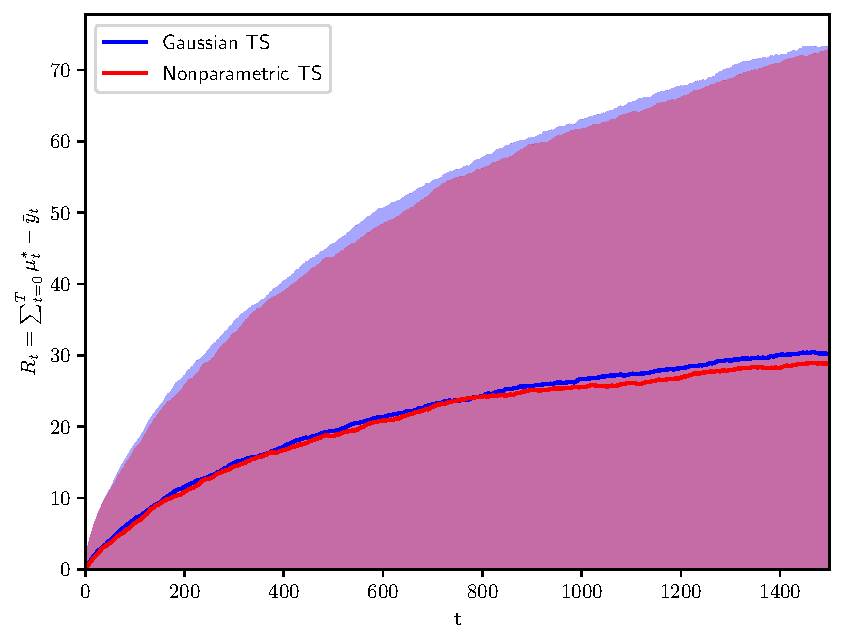
\includegraphics[width=\textwidth]{./figs/staticGaussian/cumregret_A2_-01_01_1_1}
		\vspace*{-5ex}
		\caption{$A=2$, $\theta_{1}=-0.1$, $\theta_{2}=0.1$.}
		\label{afig:static_gaussian_A2_01}
	\end{subfigure}
	\begin{subfigure}[b]{0.32\textwidth}
		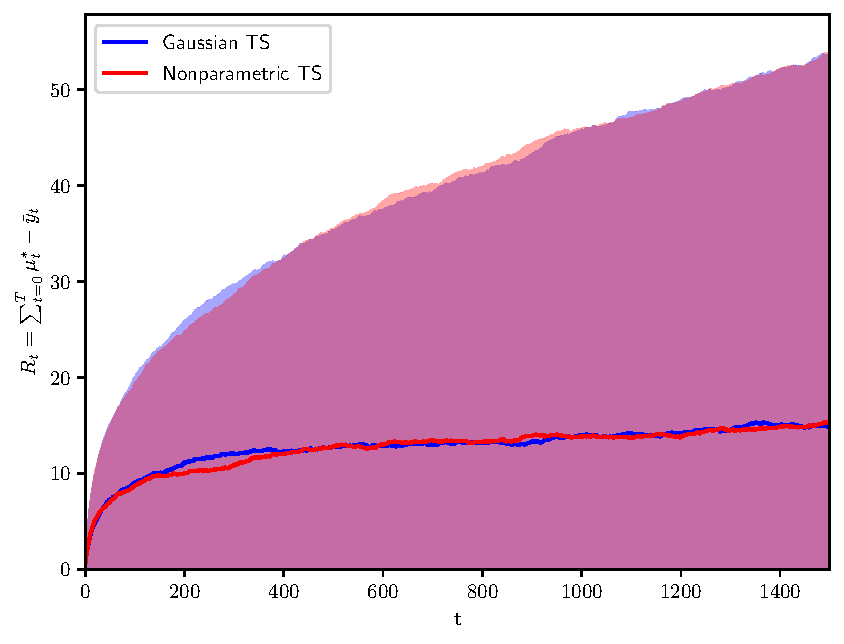
\includegraphics[width=\textwidth]{./figs/staticGaussian/cumregret_A2_-05_05_1_1}
		\vspace*{-5ex}
		\caption{$A=2$, $\theta_{1}=-0.5$, $\theta_{2}=0.5$.}
		\label{afig:static_gaussian_A2_05}
	\end{subfigure}
	\begin{subfigure}[b]{0.32\textwidth}
		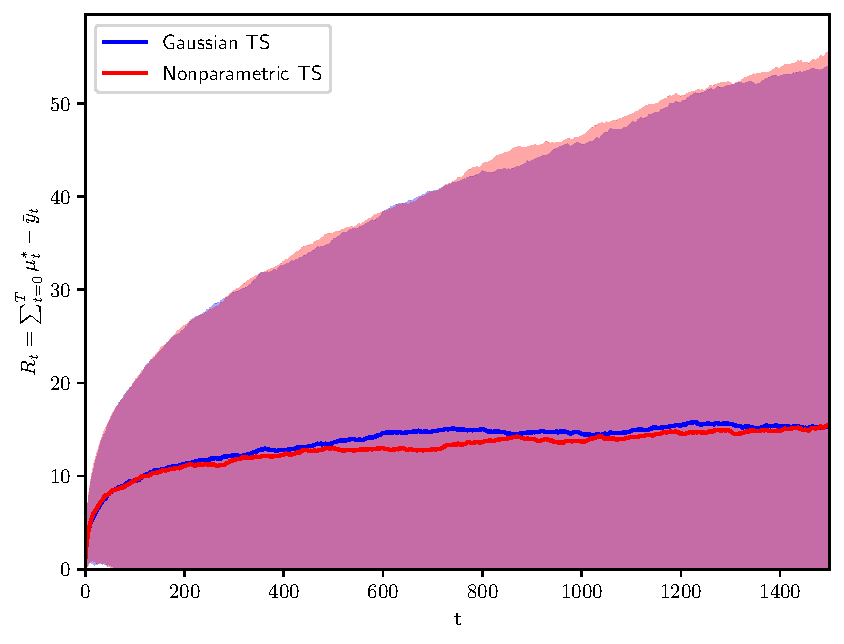
\includegraphics[width=\textwidth]{./figs/staticGaussian/cumregret_A2_-1_1_1_1}
		\vspace*{-5ex}
		\caption{$A=2$, $\theta_{1}=-1$, $\theta_{2}=1.0$.}
		\label{afig:static_gaussian_A2_1}
	\end{subfigure}
	\vspace*{-2ex}
	\caption{Mean regret (standard deviation shown as shaded region) for 1000 independent realizations of different two-armed Gaussian bandits, with $\sigma_a^2=1 \forall a$.}
	\label{afig:static_gaussian_A2}
\end{figure}

We show in Figure~\ref{afig:static_gaussian_A2} how our proposed nonparametric Thompson sampling method achieves regret comparable to that of the non-contextual Gaussian Thompson sampling as in~\cite{ip-Agrawal2012} for diverse parameterizations of such Gaussian bandits.

Recall that the non-contextual bandit scenario is seamlessly accommodated by our proposed \texttt{Nonparametric TS} algorithm by assuming a constant context, \ie $x_t=\mathds{1}$.

\section{Thompson sampling baseline hyperparameters}
\label{asec:evaluation_hyperparameters}

We here collect the specific hyperparameters used for the results presented in this work. These were selected based on the default suggested values in \href{https://github.com/tensorflow/models/tree/master/research/deep_contextual_bandits}{https://github.com/tensorflow/models/tree/master/research/deep\_contextual\_bandits}.

We first describe in Table~\ref{tab:neural_network_hyperparameters} the neural network hyperparameters, shared across all the studied alternatives but the \texttt{linearGaussian TS} and the \texttt{MultitaskGP} baselines.

\begin{table}[!h]
	\caption{Shared neural network hyperparameters.}
	\label{tab:neural_network_hyperparameters}
	\vspace*{-2ex}
	\begin{center}
		\begin{tabular}{|c|c|}
			\hline
			Hyperparameter\cellcolor[gray]{0.6} & Value \cellcolor[gray]{0.6} \\ \hline
training freq & 1 \\ \hline
training epochs & 100 \\ \hline
activation & tf.nn.relu \\ \hline
layer size & 50 \\ \hline
batch size & 512 \\ \hline
init scale & 0.3 \\ \hline
optimizer & `RMS' \\ \hline
initial pulls & 2 \\ \hline
activate decay & True \\ \hline
max grad norm & 5.0 \\ \hline
initial lr & 0.1 \\ \hline
reset lr & True \\ \hline
lr decay rate & 0.5 \\ \hline
show training & False \\ \hline
freq summary & 1000 \\ \hline
		\end{tabular}
	\end{center}
\end{table}

The specific details for each neural network based baseline are summarized in Table~\ref{tab:neural_network_baselines}, with details for the Gaussian process based baseline in Table~\ref{tab:gp_hyperparameters}.

\begin{table}[!h]
	\caption{Shared neural network hyperparameters.}
	\label{tab:neural_network_baselines} 
	\vspace*{-2ex}
	\begin{center}
	\begin{tabular}{|L{0.4\columnwidth}|J{0.5\columnwidth}|}
	\hline
Algorithm \cellcolor[gray]{0.6} & Baseline details \cellcolor[gray]{0.6} \\ \hline
\texttt{NeuralLinear}        	 & The network and the posterior parameter of the last layer are updated at every bandit iteration;
									Prior over linear parameters is $a_0=6$, $b_0=6$, $\lambda_0=0.25$ \\ \hline
\texttt{NeuralRMS}           	 & Neural network learned with RMS optimizer with default parameters \\ \hline
\texttt{NeuralBootstrapped}   	 & $q=3$ networks and datasets for bootstrapping, with $p=0.95$ \\ \hline
\texttt{NeuralParamNoise}     	 & The \iid noise added to parameters follow $\N{0,\sigma=0.05}$, and an $\epsilon=0.1$ greedy is implemented with 300 samples\\ \hline
\texttt{NeuralDropoutRMS}    	 & Dropout with parameter $0.8$ is used for training neural networks with RMS optimizer \\ \hline
\texttt{BNNVariationalGaussian}  & Variational inference over Gaussian independent weight noises with sigma exponential transform and noise $\sigma=0.1$; 100 initial training steps and 10 cleared times used in training.\\ \hline
\texttt{BNNAlphaDiv}         	 & The Black-Box method is used with $\alpha=1$, noise $\sigma=0.1$ and $k=20$, with sigma exponential transform and prior variance $\sigma^2=0.1$; 100 initial training steps and 20 cleared times used in training. \\ \hline
	\end{tabular}
	\end{center}
\end{table}

\begin{table}[!h]
	\caption{Gaussian Process hyperparameters.}
	\label{tab:gp_hyperparameters}
	\vspace*{-2ex}
	\begin{center}
		\begin{tabular}{|c|c|}
			\hline
			Hyperparameter\cellcolor[gray]{0.6} & Value \cellcolor[gray]{0.6} \\ \hline
training freq & 50 \\ \hline
training epochs & 100 \\ \hline
learn embeddings & True \\ \hline
task latent dim & 5 \\ \hline
max num points & 1000 \\ \hline
batch size & 512 \\ \hline
optimizer & `RMS' \\ \hline
initial pulls & 2 \\ \hline
lr & 0.01 \\ \hline
initial lr & 0.001 \\ \hline
lr decay rate & 0.0 \\ \hline
reset lr & False \\ \hline
activate decay & False \\ \hline
keep fixed after max obs & True \\ \hline
show training & False \\ \hline
freq summary & 1000 \\ \hline
		\end{tabular}
	\end{center}
\end{table}

\clearpage
% !TEX root = main.tex
\section{Contextual linear Gaussian bandits: baselines}
\label{asec:linearGaussian_baselines}

We show in Figure~\ref{fig:linear_gaussian_mixtures_baselines} the mean cumulative regret (and its standard deviation as the shaded region) of all the studied multi-armed bandit algorithms for diverse contextual linear Gaussian bandit parameterizations ---per-algorithm cumulative reward results are shown in Table~\ref{tab:sparse_linear_showdown_baselines_reward}.

% Linear and Sparse Gaussian reward figure
\begin{table*}[!h]
	\caption{Cumulative reward (mean and variance) at $t=1500$ for $R=500$ realizations of contextual linear Gaussian MABs.}
	\label{tab:sparse_linear_showdown_baselines_reward}
	\vspace*{-2ex}
	\begin{center}
		\resizebox{\textwidth}{!}{
		\begin{tabular}{|c|c|c|}
			\hline
			Algorithm 	\cellcolor[gray]{0.6} & Final cumulative reward (linear) \cellcolor[gray]{0.6} & Final cumulative reward (sparse linear) \cellcolor[gray]{0.6} \\ \hline
			Optimal 	 	 		& 2064.985 $\pm$ 4502.593 & 1960.926 $\pm$ 6363.005 \\ \hline
			Nonparametric TS     	 & 1875.096 $\pm$ 66.837 & 1803.519 $\pm$ 79.203 \\ \hline
			NeuralLinear         	 & 1666.499 $\pm$ 64.629 & 1626.356 $\pm$ 78.577 \\ \hline
			NeuralBootstrapped   	 & 1854.071 $\pm$ 77.620 & 1784.790 $\pm$ 87.437 \\ \hline
			NeuralRMS            	 & 1808.088 $\pm$ 93.845 & 1752.188 $\pm$ 97.987 \\ \hline
			NeuralDropoutRMS     	 & 1682.115 $\pm$ 100.281 & 1626.056 $\pm$ 113.981 \\ \hline
			NeuralParamNoise     	 & 1823.946 $\pm$ 83.025 & 1761.804 $\pm$ 96.642 \\ \hline
			MultitaskGP          	 & 1851.337 $\pm$ 64.938 & 1774.902 $\pm$ 75.291 \\ \hline
			BNNVariationalGaussian 	 & 1237.616 $\pm$ 203.954 & 1198.605 $\pm$ 215.776 \\ \hline
			BNNAlphaDiv          	 & 1271.867 $\pm$ 66.406 & 1265.829 $\pm$ 71.714 \\ \hline
		\end{tabular}
	}
	\end{center}
\end{table*}

\begin{figure}[!h]
	\centering
	\begin{subfigure}[c]{0.45\textwidth}
		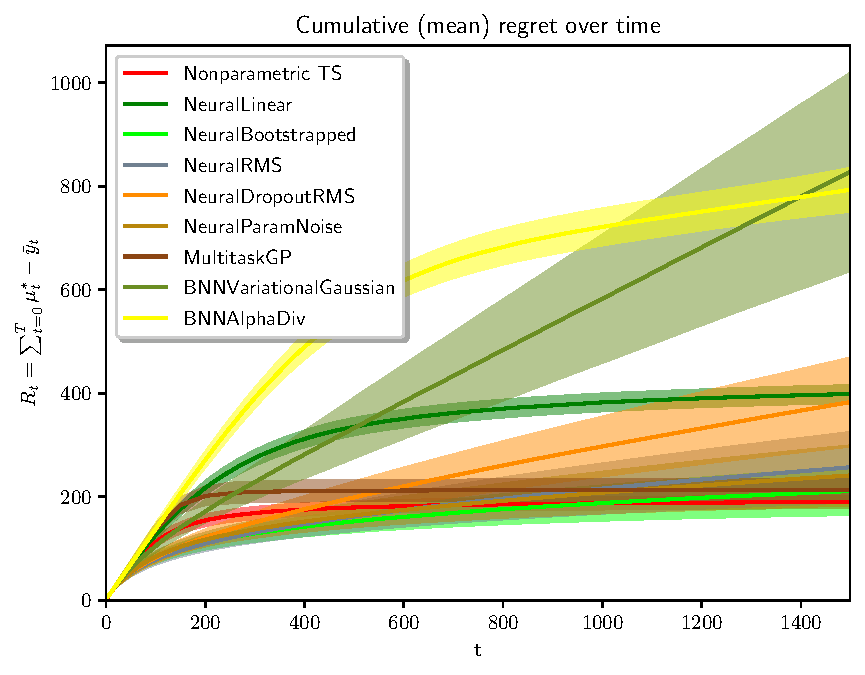
\includegraphics[width=\textwidth]{./figs/linear_showdown_baselines/cum_optexpected_regret_std}
		\vspace*{-5ex}
		\caption{Contextual linear Gaussian MAB, for $R=500$ realizations.}
		\label{fig:linear_showdown_baselines}
	\end{subfigure}
	\qquad
	\begin{subfigure}[c]{0.45\textwidth}
		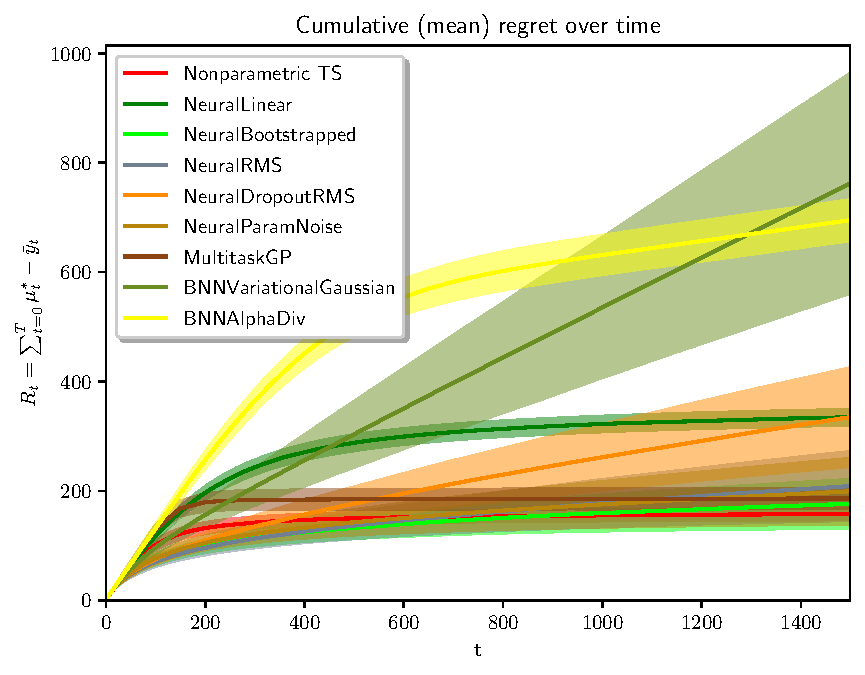
\includegraphics[width=\textwidth]{./figs/sparse_linear_showdown_baselines/cum_optexpected_regret_std}
		\vspace*{-5ex}
		\caption{Contextual sparse linear Gaussian MAB, for $R=500$ realizations.}
		\label{fig:sparse_linear_showdown_baselines}
	\end{subfigure}
	\vspace*{-2ex}
	\caption{Mean regret (standard deviation shown as shaded region) for 1000 independent realizations of the presented methods in all scenarios.}
	\label{fig:linear_gaussian_mixtures_baselines}
\end{figure}



% !TEX root = main.tex
\section{Contextual bandits not in the exponential family}
\label{asec:mixture_baselines}

We show in Table~\ref{tab:mixture_scenarios_bandit_showdown_baselines_reward} the mean (and standard deviation) cumulative regret of all the studied multi-armed bandit algorithms in the proposed complex scenarios described in Section~\ref{sssec:evaluation_mixture_scenarios_baselines}.

% Mixture bandit reward table
\begin{table*}
	\caption{Final (at $t=1000$) cumulative reward (mean and standard deviation) for $R=500$ realizations of the studied methods in all scenarios.}
	\label{tab:mixture_scenarios_bandit_showdown_baselines_reward}
	\vspace*{-2ex}
	\begin{center}
		\resizebox{\textwidth}{!}{
		\begin{tabular}{|c|c|c|c|c|}
			\hline
			Algorithm 	\cellcolor[gray]{0.6} & \texttt{Scenario A} \cellcolor[gray]{0.6} & \texttt{Scenario B} \cellcolor[gray]{0.6} & \texttt{Scenario C} \cellcolor[gray]{0.6} & \texttt{Scenario D} \cellcolor[gray]{0.6} \\ \hline
			\texttt{Optimal}       	& 2603.637 $\pm$ 43.871 & 2703.374 $\pm$ 48.053 &  2920.616 $\pm$ 47.294 &  3511.531 $\pm$ 137.860 \\ \hline
			\texttt{Nonparametric TS}  &   	 2481.226 $\pm$ 46.969 & 2064.933 $\pm$ 70.063 &  2155.669 $\pm$ 86.414 &  1916.523 $\pm$ 176.516 \\ \hline
			\texttt{LinearGaussian TS}  &   	 2477.374 $\pm$ 46.967 & 2043.161 $\pm$ 87.453 &  2124.920 $\pm$ 98.306 &  1846.032 $\pm$ 289.280 \\ \hline
			\texttt{NeuralLinear}   &      	 2474.973 $\pm$ 47.411 & 2023.889 $\pm$ 95.728 &  2102.640 $\pm$ 111.766 &  1786.915 $\pm$ 316.087 \\ \hline
			\texttt{NeuralBootstrapped} &   	 2477.389 $\pm$ 134.222 & 1959.900 $\pm$ 212.630 &  2008.643 $\pm$ 296.424 &  1846.672 $\pm$ 478.053 \\ \hline
			\texttt{NeuralRMS}         &    	 2478.773 $\pm$ 134.110 & 1953.925 $\pm$ 218.489 &  2001.024 $\pm$ 299.355 &  1808.436 $\pm$ 532.736 \\ \hline
			\texttt{NeuralDropoutRMS} &    	 2473.140 $\pm$ 165.730 & 1954.019 $\pm$ 215.282 &  2000.544 $\pm$ 302.480 &  1829.687 $\pm$ 495.924 \\ \hline
			\texttt{NeuralParamNoise} &    	 2476.161 $\pm$ 134.467 & 1970.443 $\pm$ 196.946 &  2032.456 $\pm$ 262.984 &  1822.056 $\pm$ 513.216 \\ \hline
			\texttt{MultitaskGP}      &    	 2384.541 $\pm$ 56.206 & 1954.318 $\pm$ 71.298 &  1957.400 $\pm$ 87.940 &  1332.580 $\pm$ 227.129 \\ \hline
			\texttt{BNNVariationalGaussian} & 2471.688 $\pm$ 158.345 & 1927.741 $\pm$ 176.984 &  1984.950 $\pm$ 250.108 &  1659.067 $\pm$ 388.108 \\ \hline
			\texttt{BNNAlphaDiv}       &   	 2431.362 $\pm$ 52.776 & 1904.173 $\pm$ 66.993 &  1896.702 $\pm$ 83.000 &  1751.989 $\pm$ 206.198 \\ \hline			
		\end{tabular}
	}
	\end{center}
\end{table*}


% !TEX root = main.tex
\section{Computational complexity and run-times of the evaluated Thompson sampling algorithms}
\label{asec:exec_times}
Computational cost is an important metric in real-life bandit scenarios, which motivated us to provide a computational analysis of our proposed algorithm in Section 3.2.2. As explained there, in general, the computational complexity is upper bounded by $\mathcal{O}(T \cdot Gibbs_{steps})$, which depends on the convergence criteria: \ie either the model likelihood of the sampled chain is stable within an $\epsilon$ likelihood margin between steps, or a maximum number of iterations $Gibbs_{max}$ is reached. As such, tweaking these two values controls the resulting run-times.

We provide below a comparison of the run-times incurred in the set of experiments described in the manuscript, for which we would like to raise two cautionary disclaimers:
\begin{itemize}
	\item We compare \textbf{algorithms with different implementations}: \\
	The proposed \texttt{Nonparametric TS} is implemented with standard python libraries (\ie numpy, scipy), while the rest of the algorithms are implemented in Tensorflow, as provided in the \href{https://github.com/tensorflow/models/tree/master/research/deep_contextual_bandits}{Deep Contextual bandit implementation} by~\citet{ip-Riquelme2018}. Our goal here is to introduce a new bandit algorithm, and improving the efficiency of our implementation (or coding it in Tensorflow) is out of the scope of this work.
	\item Both our algorithm and those in the \href{https://sites.google.com/site/deepbayesianbandits/}{deep contextual bandits showdown} require \textbf{updates at every time instant that depend on the number of observations per-arm $t_a$}:\\
	Performance and running-time differences can be achieved if one tweaks each algorithm's settings for model updates. As explained in~\cite{ip-Riquelme2018}, a key question is how often and for how long models are updated, as these will determine their running-times in practice. Even if ideally, one would like to re-train models after each new observation (and for as long as possible), this may limit	the applicability of the algorithms in online scenarios. In this work, we have executed all baselines based on the default hyperparameters suggested by~\citet{ip-Riquelme2018} ---which limits the retraining process per interaction to 100 epochs, upper bounding the execution time per bandit interaction--- and argue that tweaking the hyperparameters of such algorithms to reduce running-times is out of the scope of this work.
\end{itemize}

Nevertheless, and as illustrative examples, we show in Figure~\ref{afig:mixture_scenarios_bandit_showdown_exec_times} the running times of all algorithms (averaged across realizations).
First, we note that \texttt{LinearGaussian TS}, due to its conjugacy-based posterior updates that can be computed sequentially, is the fastest algorithm in all scenarios.
Second, we observe that the algorithms in~\cite{ip-Riquelme2018} have a similar running-time across all scenarios, expected due to the suggested configuration that limits per-interaction run-time to 100 epochs.
Third, the run-times of our \texttt{Nonparametric TS} algorithm vary across scenarios, as updating the nonparametric posterior model takes more or less time depending on the complexity of the true reward model: it shows low computational complexity in linear Gaussian scenarios, while incurring in higher computational cost when fitting the most challenging \texttt{Scenarios B, C}, and \texttt{D}.
However, as demonstrated in Figures~\ref{afig:scenario_A_exec_times},~\ref{afig:scenario_B_exec_times},~\ref{afig:scenario_C_exec_times} and~\ref{afig:scenario_D_exec_times}, we can drastically reduce the run-time of \texttt{Nonparametric TS} by upper-bounding the number of Gibbs iterations, yet achieve satisfactory performance, as demonstrated in Figure~\ref{fig:mixture_scenarios_bandit_showdown_gibbsmaxiter} of the manuscript.

\begin{figure*}[!h]
	\centering
	\begin{subfigure}[c]{0.45\textwidth}
		\includegraphics[width=\textwidth]{./figs/linear_showdown/exec_time_barplot}
		\vspace*{-5ex}
		\caption{Contextual linear Gaussian MAB.}
		\label{afig:linear_showdown_exec_times}
	\end{subfigure}
	\begin{subfigure}[c]{0.45\textwidth}
		\includegraphics[width=\textwidth]{./figs/sparse_linear_showdown/exec_time_barplot}
		\vspace*{-5ex}
		\caption{Contextual sparse linear Gaussian MAB.}
		\label{afig:sparse_linear_showdown_exec_times}
	\end{subfigure}
	\vspace*{-2ex}
	\caption{Mean run-time (standard deviation shown as error bars) in seconds for $R=500$ realizations  of the studied methods in linear contextual multi-armed bandits.}
	\label{afig:contextual_bandit_showdown_exec_times}
\end{figure*}

\begin{figure*}[!h]
	\centering
	\begin{subfigure}[c]{0.45\textwidth}
		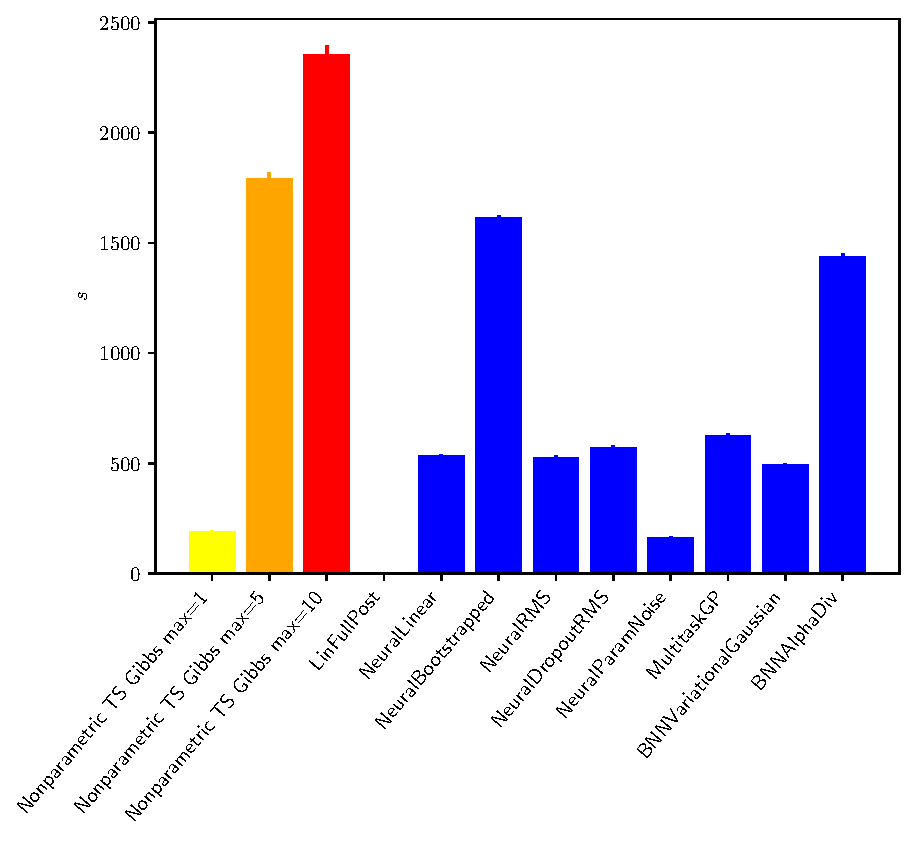
\includegraphics[width=\textwidth]{./figs/linear_gaussian_mixture_easy/exec_time_barplot}
		\vspace*{-5ex}
		\caption{\texttt{Scenario A}.}
		\label{afig:scenario_A_exec_times}
	\end{subfigure}
	\begin{subfigure}[c]{0.45\textwidth}
		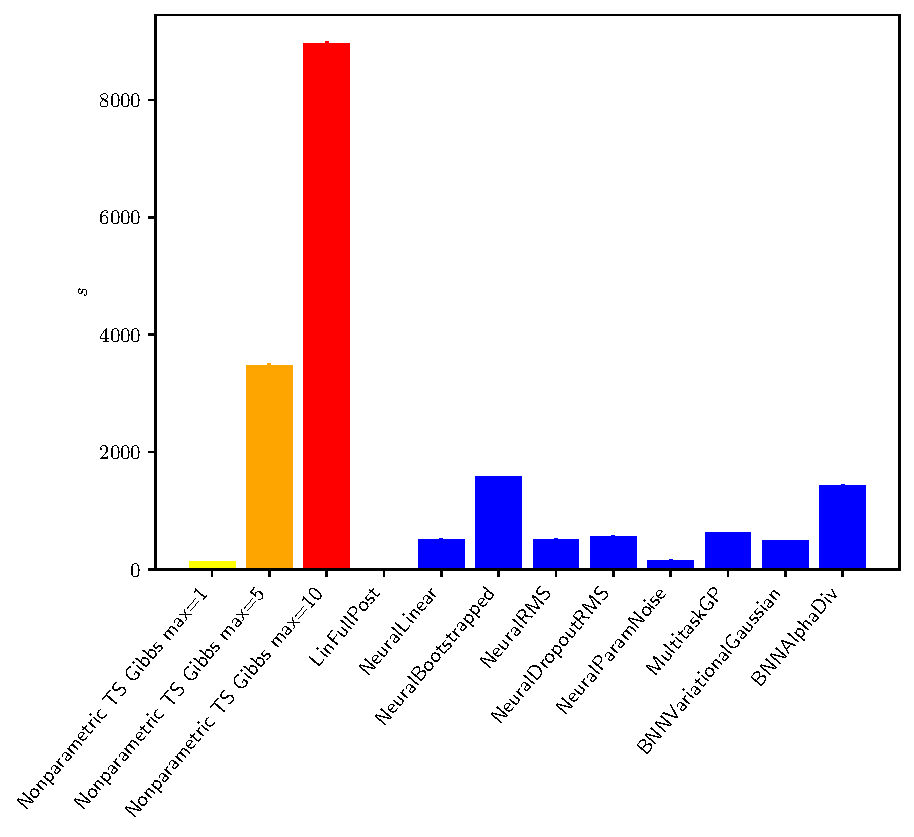
\includegraphics[width=\textwidth]{./figs/linear_gaussian_mixture_hard/exec_time_barplot}
		\vspace*{-5ex}
		\caption{\texttt{Scenario B}.}
		\label{afig:scenario_B_exec_times}
	\end{subfigure}
	
	\begin{subfigure}[c]{0.45\textwidth}
		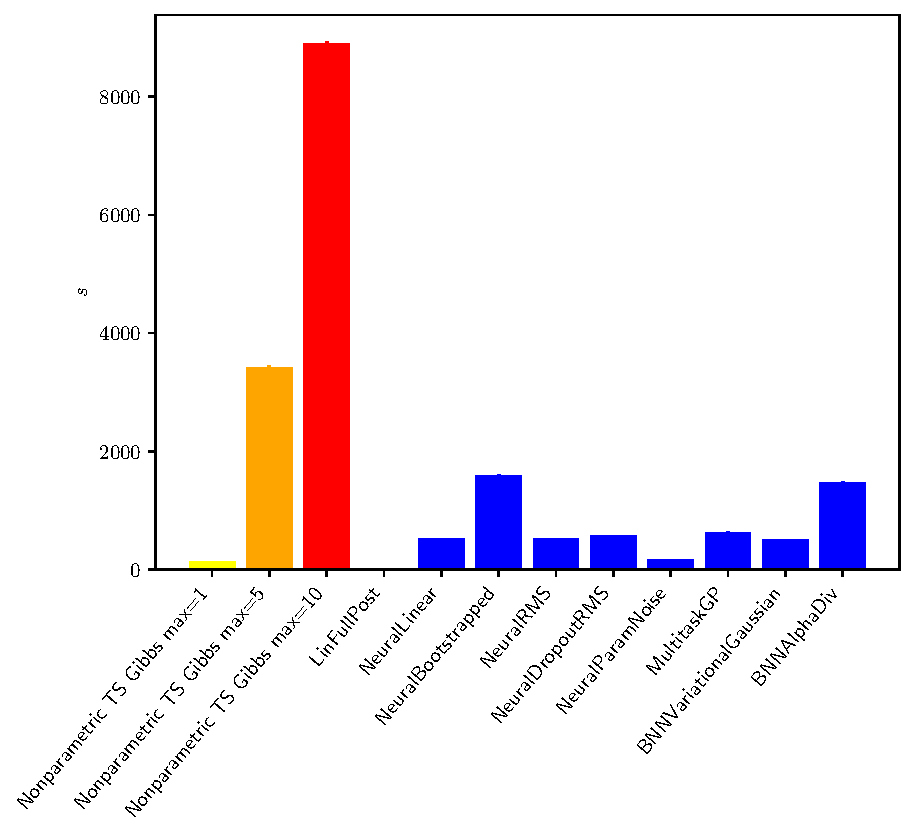
\includegraphics[width=\textwidth]{./figs/linear_gaussian_mixture_unbalanced/exec_time_barplot}
		\vspace*{-5ex}
		\caption{\texttt{Scenario C}.}
		\label{afig:scenario_C_exec_times}
	\end{subfigure}
	\begin{subfigure}[c]{0.45\textwidth}
		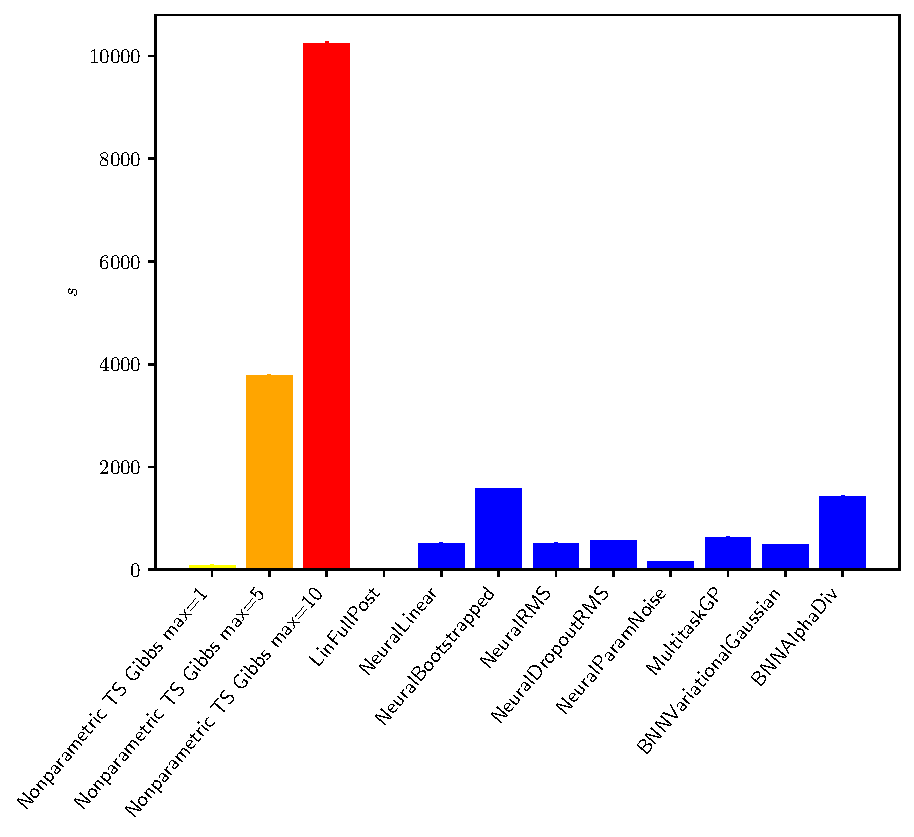
\includegraphics[width=\textwidth]{./figs/linear_gaussian_mixture_heavy_tail/exec_time_barplot}
		\vspace*{-5ex}
		\caption{\texttt{Scenario D}.}
		\label{afig:scenario_D_exec_times}
	\end{subfigure}
	\vspace*{-2ex}
	\caption{Mean run-time (standard deviation shown as error bars) in seconds for $R=500$ realizations  of the studied methods in all scenarios.}
	\label{afig:mixture_scenarios_bandit_showdown_exec_times}
\end{figure*}

We conclude by reiterating that, in general, we recommend to run the algorithm until full convergence, but suggest to limit the number of Gibbs iterations as a practical recommendation with good empirical regret performance ---analogous to the suggestion by~\citet{ip-Riquelme2018} to limit the number of per-iteration epochs for neural network based algorithms.


\end{document}
% end of file template.tex



%%%%%%%%%%%%%%%%%%%%%%%%%%%%%%%%%%%%%%%%%%%%%%%%%%%%%%%%%%%%%%%%%%%%%%%%%%%%%%%
% Appendix
\clearpage
\appendix

\section{Nonparametric hierarchical mixture model bandit}
\label{asec:nonparametric_hierarchical_mixture_model}

An alternative MAB model, where each arm is drawn from the same base distribution, is to consider a hierarchical Pitman-Yor mixture model. The generative process of a hierarchical Pitman-Yor mixture model follows:

\begin{enumerate}
\item $G_0 \sim PY(\eta,\gamma_0, H)$.
\item $G_a \sim PY(d,\gamma,G_0)$, for $a \in \mathcal{A}$.
\item $\varphi_{a,n+1} \sim G_a$, that is
\begin{equation}
\hspace*{-2ex}
\begin{cases}
m_{a,l}|m_{a,1:l-1},\gamma_0, H \sim \sum_{k=1}^{K} \frac{M_{k}-\eta}{M+\gamma_0}\delta_{\varphi_k}+\frac{\gamma_0+K\eta}{M+\gamma_0}H \;, \\
\varphi_{a,n+1}|\varphi_{a,1:n_a}, d, \gamma, G_0 \sim \sum_{l=1}^{L_a} \frac{n_{a,l}-d}{n_a+\gamma}\delta_{\varphi_{m_{a,l}}}+\frac{\gamma+L_a d}{n_a+\gamma}G_0
\end{cases}
\end{equation}
where $m_{a,l}$ refers to the per-arm $a \in \mathcal{A}$ assignments to local mixands $l_a \in \mathcal{L}_a$, each with mixture assignment $k \in \mathcal{K}$, now shared across arms. That is, there is a global mixture with $K$ mixands for the bandit, but each per-arm distribution consists of a subset of $\mathcal{L}_a \in K$ mixands.
\item The $n+1$th observation $y_{n+1}$ is drawn from the emission distribution parameterized by the parameters of its corresponding mixture component $Y_{n+1}|\varphi_{a,n+1} \sim p(Y|\varphi_{a,n+1})$.
\end{enumerate}
For parametric measures, we write $H_0(\varphi)=H(\varphi|\varPhi_0)$ and $H_n(\varphi)=H(\varphi|\varPhi_n)$, where $\varPhi_0$ are the prior hyperparameters of the emission distribution, and $\varPhi_n$ the posterior parameters after $n$ observations, respectively.
Note again that the hierarchical Dirichlet process is a particular case of the above with $d=0$.

The Gibbs sampler for inference of the above model after observations $y_{1:n}$ relies on the conditional distribution of observation assignments $c_{a,n}$ to local mixands $l \in \mathcal{L}_a$, 
\begin{equation}
\begin{cases}
p(c_{a,n+1}=l|y_{a,n+1},y_{a,1:n},c_{a,1:n}, \gamma, \gamma_0,H) \\
\hspace*{0.3\columnwidth}  \propto \frac{n_{a,l}-d}{n_a+\gamma} \int_{\varphi} p(y_{a,n+1}|\varphi_{m_{a,l}}) H_{n}(\varphi) \dd{\varphi}\\
p(c_{a,n+1}=l_{new}|y_{a,n+1},y_{a,n},c_{a,1:n},\gamma, \gamma_0, H) \\
\hspace*{0.3\columnwidth} \propto \frac{\gamma+Kd}{n_a+\gamma} \int_{\varphi} p(y_{a,n+1}|\varphi_{m_{a,l_{new}}}) H(\varphi) \dd{\varphi}\\
\hspace*{0.3\columnwidth} \propto \frac{\gamma+Kd}{n_a+\gamma} \left[ \sum_{k=1}^{K} \frac{M_{k}-\eta}{M+\gamma_0}\int_{\varphi} p(y_{a,n+1}|\varphi_{k}) H_{n}(\varphi) \dd{\varphi} \right. \\
\hspace*{0.35\columnwidth}\left. + \frac{\gamma_0 +K\eta}{M+\gamma_0} \int_{\varphi} p(y_{a,n+1}|\varphi_{k_{new}}) H(\varphi) \dd{\varphi} \right]\\
\end{cases}
\end{equation}
and mixture assignments $m_{a,l}$ for a local mixand $l\in \mathcal{L}_a$:
\begin{equation}
\begin{cases}
p(m_{a,l}=k|y_{1:n},c_{n \backslash n_{a,l}}, \gamma_0, H) \propto \frac{M_{k}-\eta}{M+\gamma_0} \int_{\varphi} p(Y_{a,l}|\varphi_{k}) H_{n \backslash n_{a,l}}(\varphi) \dd{\varphi}\\
p(m_{a,l}=k_{new}|y_{1:n},c_{n \backslash n_{a,l}}\gamma_0, H) \propto \frac{\gamma_0+K\eta}{M+\gamma_0} \int_{\varphi} p(Y_{a,l}|\varphi_{k_{new}}) H(\varphi) \dd{\varphi}
\end{cases}
\end{equation}
\begin{equation}
\begin{cases}
p(m_{a,l_{new}}=k|y_{a,n+1},y_{a,1:n},c_{a,1:n}, \gamma_0, H) \\
\hspace*{0.3\columnwidth} \propto \frac{M_{k}-\eta}{M+\gamma_0} \int_{\varphi} p(y_{a,n+1}|\varphi_{k}) H_{n}(\varphi) \dd{\varphi}\\
p(m_{a,l_{new}}=k_{new}|y_{a,n+1},y_{a,1:n},c_{a,1:n},\gamma_0, H) \\
\hspace*{0.3\columnwidth} \propto \frac{\gamma_0+K\eta}{M+\gamma_0} \int_{\varphi} p(y_{a,n+1}|\varphi_{k_{new}}) H(\varphi) \dd{\varphi}\\
\end{cases}
\end{equation}
where $n \backslash n_{a,l}$ refers to all observations but those assigned to local mixand $l$ in arm $a$, $M_k$ are the number of local mixands assigned to global mixture component $k$, and $M=\sum_{k=1}^K M_k$.

The alternative nonparametric MAB considers the above hierarchical nonparametric model, where all arms are assumed to obey the same family of distributions, but only their mixture proportions vary across arms, as illustrated in Figure~\ref{afig:pgm_nonparametric_bandit_hierarchical}.
The main advantage of this alternative is that one learns per-mixture parameter posteriors based on rewards of all played arms, with the disadvantage of all arms of the bandit being of the same family of reward distributions.

% Hierarchical nonparametric bandit graphical model
\begin{figure}[!h]
\centering
\begin{center}
	\begin{tikzpicture}
	% Nodes
	% Return y
	\node[obs] (y-t) {$y_{t}$};
	% Action a
	\node[latent, below=0.5 of y-t] (a-t) {$a_t$};
	% Context x
	\node[latent, above=0.5 of y-t]  (x-t) {$x_t$};
	% Nonparametric parameters
	\node[latent, left=0.5 of y-t, xshift=0cm] (varphi-a) {$\varphi_{a}$};
	% Nonparametric distribution
	\node[latent, left=0.5 of varphi-a, xshift=0cm] (G-a) {$G_{a}$};
	% Nonparametric shared distribution
	\node[latent, left=0.5 of G-a, xshift=0cm] (G-0) {$G_{0}$};
	
	% Hyperparameters
	% Per-arm
	\node[const, left=0.5 of G-a, yshift=-1.0cm] (d-a) {$d_{a}$} ;
	\node[const, left=0.5 of G-a, yshift=1.0cm] (gamma-a) {$\gamma_{a}$} ;
	% Shared
	\node[const, left=0.5 of G-0, yshift=-1.0cm] (d-0) {$d_{0}$} ;
	\node[const, left=0.5 of G-0, yshift=0.0cm]  (H) {$H$} ;
	\node[const, left=0.5 of G-0, yshift=1.0cm] (gamma-0) {$\gamma_{0}$} ;
	
	% Edges
	% Hyperparameters to shared distribution
	\edge {gamma-0,H} {G-0} ;
	\edge {d-0,H} {G-0} ;
	% Hyperparameters to distribution
	\edge {G-0} {G-a} ;
	\edge {gamma-a} {G-a} ;
	\edge {d-a} {G-a} ;
	% Connect distribution to parameters
	\edge {G-a} {varphi-a} ;
	% Connect parameters, context and arm to observation
	\edge {varphi-a,x-t,a-t} {y-t} ;

	% Plates
	% Over time
	\plate {t} {(a-t)(x-t)(y-t)} {$t$} ;
	% Over each arm
	\plate {a}{
		(d-a)(gamma-a)(G-a0) % hyperparameters
		(G-a) % distribution
		(varphi-a) % parameters
		(G-0.north west) (G-0.south west) % Extra space
	} {$A$} ;
\end{tikzpicture}
\end{center}
\vspace*{-2ex}
\caption{Graphical model of the hierarchical nonparametric mixture bandit distribution.}
\label{afig:pgm_nonparametric_bandit_hierarchical}
\vspace*{-2ex}
\end{figure}

% !TEX root = main.tex
\section{Asymptotic regret bound for nonparametric mixture based Thompson sampling}
\label{asec:nonparametric_thompson_sampling_regret_bound}

We start by clarifying the notation we use in the sequel:
\begin{itemize}
	\item We denote the distribution $p(\Omega)$ of the random variable $\Omega$ for the probability of a random event $\omega$ with $\myProb{p}{\Omega=\omega}$.
	\item We specify the distribution $p(\cdot)$ of the random variable within an expectation with a subscript, $\eValue{p}{\cdot}$.
	\item We use $\mu_{a}=\eValue{p}{Y_{a}}$ to indicate the expectation under some distribution $p$ of the reward for each arm $a\in\A$.
	\item We use $\mu=\{\mu_{t,a}\}, \forall a\in \A$ for the set of all per-arm expected values.
	\item We define the union of the context at time $t$ and history up to $t-1$ with $h_{1:t}=\{x_t,\HH_{1:t-1}\}$.
	\item We use $(\mu_{t,a}|h_{1:t})=\eValue{p}{Y_{a}|h_{1:t}}$ to indicate the expectation under the posterior of the reward distribution $p$ of each arm $a$ given context and history $h_{1:t}$ up to time $t$.
	%\item We denote a potentially time-varying distribution over the expected reward means as $p_{t}=p_t(\mu_t|h_{1:t})$
	\item We denote stochastic policies with $\myPi{p}{\cdot}$, where the subscript makes explicit the assumed reward model class $p(\cdot)$.
	\item For Thompson sampling policies, we may interchangeably write
\begin{align}
	\myPi{p}{A_t} &= \myPi{p}{A_t|h_{1:t}} \\
	&= \myProb{p}{A_t=a_{t}^*|h_{1:t}} \nonumber \\
	&=\myProb{p}{A_t=\argmax_{a^\prime \in \A} \left(\mu_{t,a^\prime} \big| h_{1:t}\right)} \nonumber \\ 
	& =\eValue{p}{\myind{A_t=\argmax_{a^\prime \in \A} \left(\mu_{t,a^\prime} \big| h_{1:t}\right) }} \nonumber \;.
\end{align}
	
	\item \textbf{The total variation distance} $\delta_{TV}(p,q)$ between distributions $p$ and $q$ on a sigma-algebra $\mathcal{F}$ of subsets of the sample space $\Omega$ is defined as
\begin{equation}
\delta_{TV}(p, q) = \sup_{B \in \mathcal{F}} \left|p(B)-q(B)\right| \; .
\end{equation}
When $\Omega$ is countable,
\begin{equation}
\delta_{TV}(p, q) = \sup_{B \in \mathcal{F}} \left|p(B)-q(B)\right| = \frac{1}{2} \sum_{\omega \in \Omega} \left|p(\omega) - q(\omega) \right| \; ,
\end{equation}
which is directly related to the $L1$ norm
\begin{equation}
\delta_{TV}(p, q) = \frac{1}{2} \sum_{\omega \in \Omega} \left|p(\omega) - q(\omega) \right| = \frac{1}{2} \|p-q\|_{1} \;.
\end{equation}
More broadly, if $p$ and $q$ are both absolutely continuous with respect to some base measure $\mu$,
\begin{equation}
\delta_{TV}(p, q) = \sup_{B \in \mathcal{F}} \left|p(B)-q(B)\right| = \frac{1}{2} \int_{\Omega} \left|\frac{\dd{p}}{\dd{\mu}} - \frac{\dd{q}}{\dd{\mu}} \right|  \dd{\mu} \; ,
\end{equation}
where $\frac{\dd{p}}{\dd{\mu}}$ and $\frac{\dd{q}}{\dd{\mu}}$ are the Radon-Nikodyn derivatives of $p$ and $q$ with respect to $\mu$.\\
\end{itemize}

We now re-state and proof Lemma~\ref{lemma:total_variation_bounds_diff_policies}:

% Restating Lemma1
\textbf{Lemma~\ref{lemma:total_variation_bounds_diff_policies}}:
The difference in action probabilities between two Thompson sampling policies, given the same history and context up to time $t$, is bounded by the total-variation distance $\delta_{TV}(p_t,q_t)$ between the posterior distributions of their expected rewards at time $t$, $p_t=p(\mu_{t}|h_{1:t})$ and $q_t=q(\mu_{t}|h_{1:t})$, respectively:
\begin{equation}
\myPi{p_t}{A_t=a} - \myPi{q_t}{A_t=a} \leq \delta_{TV}(p_t,q_t) \; .
\label{eq:lemma_1_equation}
\end{equation}

The proof of Lemma~\ref{lemma:total_variation_bounds_diff_policies} consists on showing that the difference between the expected values of a function of a random variable is bounded by the total variation distance between the corresponding distributions. 

\begin{proof}
	Let us define a linear function $l:\Omega \rightarrow [-1/2,1/2]$ of a bounded function $g(\omega)$:
	\begin{equation}
	l(\omega)=\frac{g(\omega)-\inf_{\omega \in \Omega} g(\omega)}{\sup_{\omega \in \Omega} g(\omega)-\inf_{\omega \in \Omega} g(\omega)} -\frac{1}{2} \; .
	\end{equation}
	Then,
	\begin{align}
	&\delta_{TV}(p, q) = \frac{1}{2} \int_{\Omega} \left|\frac{\dd{p}}{\dd{\mu}} - \frac{\dd{q}}{\dd{\mu}} \right| \dd{\mu} \geq \frac{1}{2} \int_{\Omega} \left|2 l \left(\frac{\dd{p}}{\dd{\mu}} - \frac{\dd{q}}{\dd{\mu}} \right) \right| \dd{\mu} \nonumber \\
		& \qquad  \geq \int_{\Omega} l \left(\frac{\dd{p}}{\dd{\mu}} - \frac{\dd{q}}{\dd{\mu}} \right) \dd{\mu} \geq \int_{\Omega} l \cdot \dd{p} - \int_{\Omega} l \cdot \dd{q} \nonumber \\
		& \qquad \geq \eValue{p}{l(\omega)}-\eValue{q}{l(\omega)} = \frac{\eValue{p}{g(\omega)}-\eValue{q}{g(\omega)}}{\sup_{\omega \in \Omega} g(\omega)-\inf_{\omega \in \Omega} g(\omega)} \; .
	\label{eq:total_variation_bounds_function_expectations}
	\end{align}
	We now recall that we can write the difference between two Thompson sampling policies as
	\begin{align}
	\myPi{p_t}{A} - \myPi{q_t}{A} &= \eValue{p_t}{\myind{A=\argmax_{a^\prime \in \A} \left(\mu_{t,a^\prime} \big| h_{1:t}\right)}} \nonumber \\
		&\hspace*{0.1\columnwidth}- \eValue{q_t}{\myind{A=\argmax_{a^\prime \in \A} \left(\mu_{t,a^\prime} \big| h_{1:t}\right)}} \;.
	\end{align}
	Let us define $g(\mu_{t}) = \myind{A=\argmax_{a^\prime \in \A} \left(\mu_{t,a^\prime} \big| h_{1:t}\right)}$, which is bounded in $[0,1]$:
	\begin{equation}
	\begin{cases}
	\inf_{\mu_{t}} g(\mu_{t}) = 0 \;,\\
	\sup_{\mu_{t}} g(\mu_{t}) = 1 \;.
	\end{cases}
	\end{equation} 
	Direct substitution in Equation~\eqref{eq:total_variation_bounds_function_expectations} results in	
	\begin{align}
	\delta_{TV}(p_t,q_t) &\geq \eValue{p_t}{\myind{A=\argmax_{a^\prime \in \A} \left(\mu_{t,a^\prime} \big| h_{1:t}\right)}} \nonumber \\
	&\hspace*{0.1\columnwidth}- \eValue{q_t}{\myind{A=\argmax_{a^\prime \in \A} \left(\mu_{t,a^\prime} \big| h_{1:t}\right)}} \nonumber \\
	& \geq \myPi{p_t}{A} - \myPi{q_t}{A} \;,
	\end{align}
	which concludes the proof.
\end{proof}

We make use of Lemma~\ref{lemma:total_variation_bounds_diff_policies} to bound the asymptotic expected cumulative regret of the proposed Thompson sampling with a Dirichlet process (\ie $d_a=0, \forall a$) Gaussian mixture prior. 

%\newpage
To that end, let us define the following Thompson sampling policies:
\begin{itemize}
	\item The optimal Thompson sampling policy, $\myPistar{\cdot}$, which chooses the optimal arm given the true reward model $\pstar=p(Y|\thetastar)$,
	\begin{align}
	\myPistar{\Astar_t|h_{1:t}} &=\myProb{\pstar}{\Astar_t=\argmax_{a^\prime \in \A} \left(\mu_{t,a^\prime} \big| h_{1:t}\right)} \nonumber \\ 
	&= \eValue{\pstar}{\myind{\Astar_t=\argmax_{a^\prime \in \A} \left(\mu_{t,a^\prime} \big| h_{1:t}\right) }} \;.
	\end{align}
	%The actions of the optimal policy, denoted as $\Astar_t\sim \myPistar{\Astar_t}$, are stochastic due to the uncertainty on the true model $\pstar$.
	\item A parametric Thompson sampling policy, $\myPi{p}{\cdot}$, which knows the true reward distribution model class $p=p(Y|\theta)$, but not the true parameter $\thetastar$,
	\begin{align}
	\myPi{p}{A_t|h_{1:t}}&=\myProb{p}{A_t=\argmax_{a^\prime \in \A} \left(\mu_{t,a^\prime} \big| h_{1:t}\right)} \nonumber \\ 
	& =\eValue{p}{\myind{A_t=\argmax_{a^\prime \in \A} \left(\mu_{t,a^\prime} \big| h_{1:t}\right) }} \;.
	\end{align}
	The actions of this Thompson sampling policy, denoted as $A_t\sim \myPi{p}{A_t|h_{1:t}}$, are stochastic due to the uncertainty on the parameter $\theta$ of the true density $p(Y|\theta)$.
	\item A nonparametric Thompson sampling policy, $\myPitilde{\cdot}$, which estimates the unknown true reward distribution with a nonparametric density $\ptilde=\ptilde(Y|\varphi)$,
	\begin{align}
	\myPitilde{\Atilde_t|h_{1:t}} &=\myProb{\ptilde}{\Atilde_t=\argmax_{a^\prime \in \A} \left(\mu_{t,a^\prime} \big| h_{1:t}\right)} \nonumber \\ 
	&=\eValue{\ptilde}{\myind{\Atilde_t=\argmax_{a^\prime \in \A} \left(\mu_{t,a^\prime} \big| h_{1:t}\right) }} \;.
	\end{align}
	The actions of this Thompson sampling policy, denoted as $\Atilde_t\sim \myPitilde{\Atilde_t|h_{1:t}}$, are stochastic due to the uncertainty on the parameter $\varphi$ of the nonparametric density $\ptilde(Y|\theta)$.
\end{itemize}

\textbf{Theorem~\ref{th:regret_bound}}:
The expected cumulative regret at time $T$ of a Dirichlet process Gaussian mixture model based Thompson sampling algorithm is asymptotically bounded by
	\begin{equation}
	R_T	=\eValue{}{\sum_{t=1}^T Y_{t,\Astar_t}-Y_{t,\Atilde_t} } \leq \mathcal{O}\left(|\A| \log^\kappa T \sqrt{T} \right) \; \text{ as } T \rightarrow \infty \;,
	\end{equation}
	where the expectations are taken over the random rewards $Y_t\sim \pstar=p(Y|x_t,\thetastar)$ and the random actions of the stochastic policies $\myPistar{\Astar_t}$ and $\myPitilde{\Atilde_t}$.
	
	This expected regret bound holds in the frequentist sense.

	We use big-O notation $\mathcal{O}(\cdot)$ as it bounds from above the growth of the cumulative regret over time for large enough input sizes, \ie
\begin{align}
\lim_{T\rightarrow \infty} \frac{R_T}{|\A| \log^\kappa T \sqrt{T} } & \leq \mathcal{O}(1)\; .
\end{align}

In the following, we avoid notation clutter and denote $\pstar=\pstar(Y)=p(Y|\thetastar)$ for the true reward distribution given the true parameters $\thetastar$, and drop the dependency over the observed history $h_{1:t}$ at time $t$ in the considered Thompson sampling policies: 
$\pi_{\pstar}=\myPistar{\Astar_t|h_{1:t}}$, for the optimal Thompson sampling policy with knowledge of the true reward model $\pstar=p(Y|\thetastar)$;
$\pi_{p}= \myPi{p}{A_t|h_{1:t}}$, for a Thompson sampling policy with knowledge of the true reward distribution model class $p=p(Y|\theta)$ ---but not the true parameter $\thetastar$; and 
$\pi_{\ptilde}=\myPitilde{\Atilde_t|h_{1:t}}$, for a nonparametric Thompson sampling policy that estimates the unknown true reward distribution with a nonparametric density $\ptilde=\ptilde(Y|\varphi)$.


\begin{proof}
\begin{align}
R_T &=\eValue{}{\sum_{t=1}^T Y_{t,\Astar_t}-Y_{t,\Atilde_t} } \label{eq:cum_regret_optimal_to_nts} \\
&=\eValue{\pi_{\pstar},\pi_{\ptilde}}{\eValue{\pstar}{
		\sum_{t=1}^T Y_{t,\Astar_t}-Y_{t,\Atilde_t} 
	}
	} \\
&=\sum_{t=1}^T \eValue{\pi_{\pstar},\pi_{\ptilde}}{\eValue{\pstar}{ Y_{t,\Astar_t}-Y_{t,\Atilde_t}}} \\
&=\sum_{t=1}^T \eValue{\pi_{\pstar},\pi_{\ptilde},\pi_{p}}{\eValue{\pstar}{ Y_{t,\Astar_t}-Y_{t,A_t}+Y_{t,A_t}-Y_{t,\Atilde_t}}} \\
&=\sum_{t=1}^T \eValue{\pi_{\pstar},\pi_{p}}{\eValue{\pstar}{ Y_{t,\Astar_t}-Y_{t,A_t}}} \nonumber \\
& \qquad + \sum_{t=1}^T \eValue{\pi_{p},\pi_{\ptilde}}{\eValue{\pstar}{ Y_{t,A_t}-Y_{t,\Atilde_t}}} \\
&=\sum_{t=1}^T \eValue{\pi_{\pstar},\pi_{p}}{\mu_{t,\Astar_t}-\mu_{t,A_t} } \nonumber \\
& \qquad + \sum_{t=1}^T \eValue{\pi_{p},\pi_{\ptilde}}{\mu_{t,A_t}-\mu_{t,\Atilde_t} } \; , \label{eq:cum_regret_nts} 
\end{align}
where we have split the expected cumulative regret of \autoref{eq:cum_regret_optimal_to_nts} in two terms.

The first term in the RHS of \autoref{eq:cum_regret_nts} relates to the regret between the optimal policy $\Astar_t \sim \myPistar{\Astar_t|h_{1:t}}$ and a Thompson sampling policy that knows the true model class $A_t \sim \myPi{p}{A_t|h_{1:t}}$; and the second term in the RHS of \autoref{eq:cum_regret_nts} accommodates the regret between a Thompson sampling policy that knows the true model class $A_t \sim \myPi{p}{A_t|h_{1:t}}$, and a Thompson sampling that estimates reward functions via nonparametric processes $\Atilde_t \sim \myPitilde{\Atilde_t|h_{1:t}}$.

Let us first work on the first term in the RHS of \autoref{eq:cum_regret_nts}:
\begin{align}
&\sum_{t=1}^T \eValue{\pi_{\pstar},\pi_{p}}{\mu_{t,\Astar_t}-\mu_{t,A_t} } \\
&\qquad =\sum_{t=1}^T \left[ \left(\sum_{\astar_t \in \A}\mu_{t,\astar_t} \myPistar{\Astar_t=\astar_t|h_{1:t}}\right) \right. \\
&\qquad \qquad \qquad  \left. - \left( \sum_{a_t \in \A}\mu_{t,a_t} \myPi{p}{A_t=a_t|h_{1:t}}\right)\right]\\
&\qquad =\sum_{t=1}^T \left(\sum_{a \in \A} \mu_{t,a} \left[\myPistar{\Astar_t=a|h_{1:t}}-\myPi{p}{A_t=a|h_{1:t}}\right] \right) \\
&\qquad \leq \sum_{t=1}^T \left(\sum_{a \in \A} C_A \left[\myPistar{\Astar_t=a|h_{1:t}}-\myPi{p}{A_t=a|h_{1:t}}\right]  \right) \label{eq:cum_regret_optimal_to_ts_C_A} \\
&\qquad \leq \sum_{t=1}^T \left(\sum_{a \in \A} C_A \delta_{TV} \left(\pstar(\mu_t|h_{1:t}),p(\mu_t|h_{1:t})\right) \right) \label{eq:cum_regret_optimal_to_ts_total_variation} \\
&\qquad \leq  \sum_{t=1}^T \sum_{a \in \A} C_A C_p t^{-1/2} \label{eq:cum_regret_optimal_to_ts_total_variation_convergence} \\
&\qquad \leq C_A C_p \sum_{a \in \A} \left(\sum_{t=1}^{T} t^{-1/2} \right) \label{eq:cum_regret_optimal_to_ts_rearrange_sum} \\
&\qquad \leq C_A C_p \sum_{a \in \A} \left(\int_{t=1}^{T} t^{-1/2} \dd{t} \right) \label{eq:cum_regret_optimal_to_ts_sum_t_integral} \\
&\qquad \leq C_A C_p \sum_{a \in \A} (2 \sqrt{T} - 2) \label{eq:cum_regret_optimal_to_ts_algebra_on_t_integral_solution} \\
&\qquad \leq 2 C_A C_p |\A| \sqrt{T} \; ,\label{eq:cum_regret_optimal_to_ts_algebra_on_t_sum_a}
\end{align}

where
\begin{itemize}
	\item in \autoref{eq:cum_regret_optimal_to_ts_C_A}: we define $C_A \coloneqq \max_{a \in \A} \mu_{a,t}, \forall t$, \ie it is an upper bound on the expected rewards of the bandit.
	
	\item in \autoref{eq:cum_regret_optimal_to_ts_total_variation}: by direct application of \autoref{eq:lemma_1_equation} in Lemma~\ref{lemma:total_variation_bounds_diff_policies}:
	$\myPistar{\Astar_t=a|h_{1:t}}-\myPi{p}{A_t=a|h_{1:t}} \leq \delta_{TV} \left(\pstar(\mu_t|h_{1:t}),p(\mu_t|h_{1:t})\right)$.
	
	That is, the difference in probabilities of playing each arm $a$ are bounded by the total variation distance between the posterior distributions of the expected rewards for each policy.
	
	For the optimal Thompson sampling policy, the parameters of the reward distribution are known, \ie the posterior is a delta at the true $\thetastar$ value:
	\begin{align}
		\pstar(\mu_t|h_{1:t}) &=\int_{\thetastar}\pstar(\mu_t|\thetastar)p(\thetastar|h_{1:t})\dd\thetastar \nonumber \\
		&=\int_{\thetastar}\pstar(\mu_t|\thetastar)\delta(\thetastar)\dd\thetastar \nonumber \\ 
		&= \pstar(\mu_t|\thetastar) \nonumber \;.
	\end{align}
	
	For the Thompson sampling policy that knows the true model class, the parameters of the reward distribution are updated as history $h_{1:t}$ is observed:
	\begin{align}
	p(\mu_t|h_{1:t}) &=\int_{\theta} p(\mu_t|\theta)p(\theta|h_{1:t})\dd\theta \nonumber \;.
	\end{align}
	
	\item in \autoref{eq:cum_regret_optimal_to_ts_total_variation_convergence}: $\delta_{TV} \left(\pstar(\mu_t|h_{1:t}),p(\mu_t|h_{1:t})\right) \sim C_p t^{-1/2}$, as $t \rightarrow \infty$, where $C_p$ is a constant that depends on the properties of the parameterized distributions, and does not depend on the amount of observed data. \\
	As explained in \citep{j-Ghosal2000}, for a class of parameterized distributions $\mathcal{P}=\{p(Y|\theta)\}_{\theta \in \Theta}$ and a prior constructed by putting a measure on the parameter set $\Theta$, it is well known that the posterior distribution of $\theta$ asymptotically achieves the optimal rate of convergence under mild regularity conditions ---\ie $\Theta$ is subset of a finite-dimensional Euclidean space, and the prior and model dependence is sufficiently regular \citep{b-Ibragimov1981}.
	In particular, and according to the Bernstein-von Mises theorem, if the model $p(Y|\theta)$ is suitably differentiable, then the convergence rate of the posterior mean $p(\mu_t|h_{1:t})$ and $\pstar(\mu_t)$ is of order $t^{-1/2}$, where $t$ indicates the amount of \iid data drawn from the true distribution $\pstar(Y)$.
	
	Note that the true $\pstar(\mu_t)$ and the posterior $p(\mu_t|h_{1:t})$ are over the expected rewards of all arms.
	Therefore, $t=\sum_{a \in \A} t_a$, where $t_a$ indicates the number of observations for each arm, is the number of times all arms $\forall a\in \A$ have been pulled.
	Consequently, the total variation \autoref{eq:cum_regret_optimal_to_ts_total_variation_convergence} depends on the total number of observations $t$ across all arms $a$.
	
	\item in \autoref{eq:cum_regret_optimal_to_ts_sum_t_integral}: $\sum_{t=1}^{T} t^{-1/2} = \mathbb{H}^{1/2}(T)\leq \int_{t=1}^{T} t^{-1/2} \dd{t}$, where $\mathbb{H}$ is the generalized harmonic number of order $1/2$ of $T$. 
\end{itemize}

This concludes the proof of the bound of the first term in the RHS of \autoref{eq:cum_regret_nts}.

\pagebreak
We now bound the second term in the RHS:

\begin{align}
&\sum_{t=1}^T \eValue{\pi_{p},\pi_{\ptilde}}{\mu_{t,A_t}-\mu_{t,\Atilde_t} } \\
&\qquad =\sum_{t=1}^T \left[ \left(\sum_{a_t \in \A}\mu_{t,a_t} \myPi{p}{A_t=a_t|h_{1:t}}\right) \right. \\
&\qquad \qquad \qquad \left. - \left( \sum_{\atilde_t \in \A}\mu_{t,\atilde_t} \myPitilde{\Atilde_t=\atilde_t|h_{1:t}}\right) \right] \\
&\qquad =\sum_{t=1}^T \left(\sum_{a \in \A} \mu_{t,a} \left[\myPi{p}{A_t=a|h_{1:t}}-\myPitilde{\Atilde_t=a|h_{1:t}}\right] \right) \\
&\qquad \leq \sum_{t=1}^T \left(\sum_{a \in \A} C_A \left[\myPi{p}{A_t=a|h_{1:t}}-\myPitilde{\Atilde_t=a|h_{1:t}}\right]  \right) \label{eq:cum_regret_ts_to_nts_C_A} \\
&\qquad \leq \sum_{t=1}^T \left(\sum_{a \in \A} C_A \delta_{TV} \left(p(\mu_t|h_{1:t}),\ptilde(\mu_t|h_{1:t})\right) \right) \label{eq:cum_regret_ts_to_nts_total_variation} \\
&\qquad \leq \sum_{t=1}^T \sum_{a \in \A} C_A C_{\ptilde} t^{-1/2}(\log t)^\kappa \label{eq:cum_regret_ts_to_nts_total_variation_convergence} \\
&\qquad \leq C_A C_{\ptilde} \sum_{a \in \A} \left(\sum_{t=1}^{T} t^{-1/2} (\log T)^\kappa \right) \label{eq:cum_regret_ts_to_nts_rearrange_sum_bound_logT} \\
&\qquad \leq C_A C_{\ptilde} \sum_{a \in \A} (\log T)^\kappa \left(\int_{t=1}^{T} t^{-1/2} \dd{t} \right) \label{eq:cum_regret_ts_to_nts_sum_t_integral} \\
&\qquad \leq C_A C_{\ptilde} \sum_{a \in \A} (\log T)^\kappa (2 \sqrt{T} - 2) \label{eq:cum_regret_ts_to_nts_algebra_on_t_integral_solution} \\
&\qquad \leq 2 C_A C_{\ptilde} |\A| (\log T)^\kappa\sqrt{T} \; , \label{eq:cum_regret_ts_to_nts_algebra_on_t_sum_a} 
\end{align}

where

\begin{itemize}
	\item in \autoref{eq:cum_regret_ts_to_nts_C_A}: $C_A \coloneqq \max_{a \in \A} \mu_{a,t}, \forall t$, as above.

	\item in \autoref{eq:cum_regret_ts_to_nts_total_variation}: by direct application of \autoref{eq:lemma_1_equation} in Lemma~\ref{lemma:total_variation_bounds_diff_policies}:
	$\myPi{p}{A_t=a|h_{1:t}}-\myPitilde{\Atilde_t=a|h_{1:t}} \leq \delta_{TV} \left(p(\mu_t|h_{1:t}),\ptilde(\mu_t|h_{1:t})\right)$.
	
	That is, the difference in probabilities of playing each arm $a$ are bounded by the total variation distance between the posterior distributions of the expected rewards for each policy.

	For the Thompson sampling policy that knows the true model class, the parameters of the reward distribution are updated as history $h_{1:t}$ is observed:
	\begin{align}
	p(\mu_t|h_{1:t}) &=\int_{\theta} p(\mu_t|\theta)p(\theta|h_{1:t})\dd\theta \nonumber \;.
	\end{align}
	
	For the Thompson sampling that estimates reward functions via nonparametric model $\ptilde(Y_t|\varphi)$, the parameters $\varphi$ of the nonparametric reward distribution are updated as history $h_{1:t}$ is observed:
	\begin{align}
	\ptilde(\mu_t|h_{1:t}) &=\int_{\varphi} \ptilde(\mu_t|\varphi)\ptilde(\varphi|h_{1:t})\dd\varphi \nonumber \;.
	\end{align}

	\item in \autoref{eq:cum_regret_ts_to_nts_total_variation_convergence}: $\delta_{TV} \left(p(\mu_t|h_{1:t}),\ptilde(\mu_t|h_{1:t})\right) \sim C_{\ptilde} t^{-1/2}(\log t)^\kappa$, as $t\rightarrow \infty$; 
	where $C_{\ptilde}$ is a constant that depends on the properties of both the true parametric posterior distribution and the nonparametric prior model, but does not depend on the amount of observed data. 
	We asymptotically bound the total variation distance between the true parametric posterior distribution and a nonparametric model-based posterior distribution, leveraging state-of-the-art results.
	
	Note that the posterior $p(\mu_t|h_{1:t})$ is over the expected rewards over all arms. Therefore, \autoref{eq:cum_regret_ts_to_nts_total_variation_convergence} depends on the total number of observations across all arms $t=\sum_{a \in \A} t_a$, where $t_a$ indicates the number of observations observed for each arm $\forall a\in \A$.
	
	The behavior of posterior distributions for infinite dimensional models has been thoroughly studied at the beginning of this century, with work by~\citet{j-Ghosal2001,j-Ghosal2007} providing posterior convergence rates of Dirichlet process Gaussian mixtures to different mixture distributions.
	
	For example, for a mixture of normals with standard deviations bounded by two positive numbers, ~\citet{j-Ghosal2001} show that the Hellinger distance between the nonparametric posterior given $n$ data samples and the true distribution is asymptotically bounded,
	\begin{equation}
	d(\ptilde,\pstar) \leq M n^{-1/2}(\log n)^\kappa \; ,
	\label{eq:nonparametric_basic_bound}
	\end{equation}
	where the value $\kappa \geq 0$ depends on the choices of priors over the location and scale of the mixtures, and data is drawn from the true distribution $\pstar$. Since $\|p-q\|_1 \leq 2 d(p,q)$, bounds in Hellinger distance apply to total variation distance as well. Note that the convergence of the posterior at such rate also implies that there exist estimators, such as the posterior mean, that converge at the same rate in the frequentist sense.
	
	Technical details of the bound in Equation~\eqref{eq:nonparametric_basic_bound} can be found in~\citep{j-Ghosal2001}, where they consider Gaussian location mixtures and location-scale mixtures, assumed the standard deviations to be bounded away from zero and infinity, and that the true mixing distribution of the location is compactly supported or has sub-Gaussian tails.
	
	A rate with $\kappa=1$ is obtained when a compactly supported base measure is used for the location prior (and the scale prior has a continuous and positive density on an interval containing the true scale parameter).
	For the commonly used normal base measure, the bound yields a rate $O(n^{-1/2}(\log n)^{3/2})$.
	When the base measure is the product of a normal distribution with a distribution supported within the range of the true scale, such that the density is positive on a rectangle containing the true location-scale space, the rate results in $O(n^{-1/2}(\log n)^{7/2})$.
	
	Later work by~\citet{j-Ghosal2007} provides new posterior convergence rates for densities that are twice continuously differentiable, where under some regularity conditions, the posterior distribution based on a Dirichlet mixture of normal prior attains a convergence rate of $O(n^{-2/5}(\log n)^{4/5})$.
	As such, it seems reasonable that the power of the logarithm, \ie $\kappa$ in Equation~\eqref{eq:nonparametric_basic_bound}, can be improved.
	~\citet{j-Ghosal2007} argue that, by using a truncated inverse gamma prior on the scale of the Gaussian mixtures, a nearly optimal convergence rate is obtained ---for which one would need to extend the Gibbs sampler with an additional accept-reject step to take care of the scale truncation.
	
	All these bounds would not be directly applicable if the true data generating density would not be part of the model classes considered.
	However, ~\citet{j-Ghosal2001} argue that a rate for these cases may as well be calculated, but since they may not be close to the optimal rate, have not been pursued yet.

	\item in \autoref{eq:cum_regret_ts_to_nts_rearrange_sum_bound_logT}: $(\log t)^{\kappa} \leq (\log T)^{\kappa}, \forall 1 \leq t \leq T, \kappa \geq 0$.

	\item in \autoref{eq:cum_regret_ts_to_nts_sum_t_integral}: $\sum_{t=1}^{T} t^{-1/2} = \mathbb{H}^{1/2}(T)\leq \int_{t=1}^{T} t^{-1/2} \dd{t}$, where $\mathbb{H}$ is the generalized harmonic number of order $1/2$ of $T$. 
\end{itemize}

%\newpage
Combining the above results, we can now bound the asymptotic cumulative regret in \autoref{eq:cum_regret_optimal_to_nts}, for a nonparametric Thompson sampling policy with Dirichlet process Gaussian mixtures, with priors and data-generating densities that meet the necessary regularity conditions:
\vspace*{-1ex}
\begin{align}
R_T 
&=\sum_{t=1}^T \eValue{\pi_{\pstar},\pi_{p}}{\eValue{\pstar}{ Y_{t,\Astar_t}-Y_{t,A_t}}} \nonumber \\
& \qquad + \sum_{t=1}^T \eValue{\pi_{p},\pi_{\ptilde}}{\eValue{\pstar}{ Y_{t,A_t}-Y_{t,\Atilde_t}}} \\
&\leq \mathcal{O} \left(2 C_A C_p |\A| \sqrt{T} + 2 C_A C_{\ptilde} |\A| (\log T)^\kappa\sqrt{T} \right)\\
&\leq \mathcal{O} \left(2 C_A |\A| \sqrt{T} (C_p + C_{\ptilde} (\log T)^\kappa ) \right) \\
&\leq \mathcal{O} |\A| \sqrt{T} (\log T)^\kappa \;.
\end{align}
We note that this bound holds both in a frequentist and Bayesian view of expected cumulative regret.
\end{proof} 



\clearpage
% !TEX root = main.tex
\section{Non-contextual Gaussian bandits: comparison to the Oracle TS}
\label{asec:noncontextual_gaussian_bandits}

\begin{figure}[!h]
	\centering
	\begin{subfigure}[b]{0.32\textwidth}
		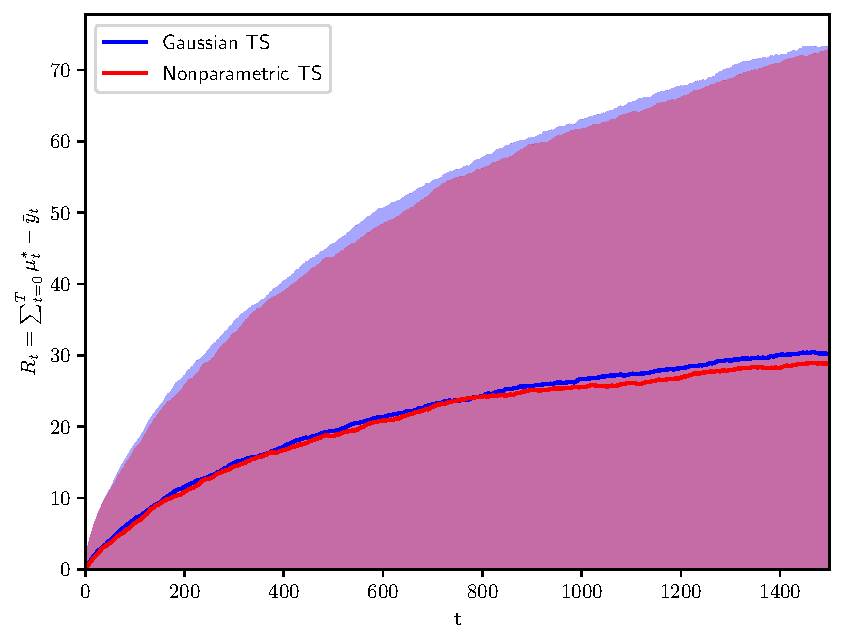
\includegraphics[width=\textwidth]{./figs/staticGaussian/cumregret_A2_-01_01_1_1}
		\vspace*{-5ex}
		\caption{$A=2$, $\theta_{1}=-0.1$, $\theta_{2}=0.1$.}
		\label{afig:static_gaussian_A2_01}
	\end{subfigure}
	\begin{subfigure}[b]{0.32\textwidth}
		\includegraphics[width=\textwidth]{./figs/staticGaussian/cumregret_A2_-05_05_1_1}
		\vspace*{-5ex}
		\caption{$A=2$, $\theta_{1}=-0.5$, $\theta_{2}=0.5$.}
		\label{afig:static_gaussian_A2_05}
	\end{subfigure}
	\begin{subfigure}[b]{0.32\textwidth}
		\includegraphics[width=\textwidth]{./figs/staticGaussian/cumregret_A2_-1_1_1_1}
		\vspace*{-5ex}
		\caption{$A=2$, $\theta_{1}=-1$, $\theta_{2}=1.0$.}
		\label{afig:static_gaussian_A2_1}
	\end{subfigure}
	\vspace*{-2ex}
	\caption{Mean regret (standard deviation shown as shaded region) for 1000 independent realizations of different two-armed Gaussian bandits, with $\sigma_a^2=1 \forall a$.}
	\label{afig:static_gaussian_A2}
\end{figure}

We show in Figure~\ref{afig:static_gaussian_A2} how our proposed nonparametric Thompson sampling method achieves regret comparable to that of the non-contextual Gaussian Thompson sampling as in~\cite{ip-Agrawal2012} for diverse parameterizations of such Gaussian bandits.

Recall that the non-contextual bandit scenario is seamlessly accommodated by our proposed \texttt{Nonparametric TS} algorithm by assuming a constant context, \ie $x_t=\mathds{1}$.

\section{Thompson sampling baseline hyperparameters}
\label{asec:evaluation_hyperparameters}

We here collect the specific hyperparameters used for the results presented in this work. These were selected based on the default suggested values in \href{https://github.com/tensorflow/models/tree/master/research/deep_contextual_bandits}{https://github.com/tensorflow/models/tree/master/research/deep\_contextual\_bandits}.

We first describe in Table~\ref{tab:neural_network_hyperparameters} the neural network hyperparameters, shared across all the studied alternatives but the \texttt{linearGaussian TS} and the \texttt{MultitaskGP} baselines.

\begin{table}[!h]
	\caption{Shared neural network hyperparameters.}
	\label{tab:neural_network_hyperparameters}
	\vspace*{-2ex}
	\begin{center}
		\begin{tabular}{|c|c|}
			\hline
			Hyperparameter\cellcolor[gray]{0.6} & Value \cellcolor[gray]{0.6} \\ \hline
training freq & 1 \\ \hline
training epochs & 100 \\ \hline
activation & tf.nn.relu \\ \hline
layer size & 50 \\ \hline
batch size & 512 \\ \hline
init scale & 0.3 \\ \hline
optimizer & `RMS' \\ \hline
initial pulls & 2 \\ \hline
activate decay & True \\ \hline
max grad norm & 5.0 \\ \hline
initial lr & 0.1 \\ \hline
reset lr & True \\ \hline
lr decay rate & 0.5 \\ \hline
show training & False \\ \hline
freq summary & 1000 \\ \hline
		\end{tabular}
	\end{center}
\end{table}

The specific details for each neural network based baseline are summarized in Table~\ref{tab:neural_network_baselines}, with details for the Gaussian process based baseline in Table~\ref{tab:gp_hyperparameters}.

\begin{table}[!h]
	\caption{Shared neural network hyperparameters.}
	\label{tab:neural_network_baselines} 
	\vspace*{-2ex}
	\begin{center}
	\begin{tabular}{|L{0.4\columnwidth}|J{0.5\columnwidth}|}
	\hline
Algorithm \cellcolor[gray]{0.6} & Baseline details \cellcolor[gray]{0.6} \\ \hline
\texttt{NeuralLinear}        	 & The network and the posterior parameter of the last layer are updated at every bandit iteration;
									Prior over linear parameters is $a_0=6$, $b_0=6$, $\lambda_0=0.25$ \\ \hline
\texttt{NeuralRMS}           	 & Neural network learned with RMS optimizer with default parameters \\ \hline
\texttt{NeuralBootstrapped}   	 & $q=3$ networks and datasets for bootstrapping, with $p=0.95$ \\ \hline
\texttt{NeuralParamNoise}     	 & The \iid noise added to parameters follow $\N{0,\sigma=0.05}$, and an $\epsilon=0.1$ greedy is implemented with 300 samples\\ \hline
\texttt{NeuralDropoutRMS}    	 & Dropout with parameter $0.8$ is used for training neural networks with RMS optimizer \\ \hline
\texttt{BNNVariationalGaussian}  & Variational inference over Gaussian independent weight noises with sigma exponential transform and noise $\sigma=0.1$; 100 initial training steps and 10 cleared times used in training.\\ \hline
\texttt{BNNAlphaDiv}         	 & The Black-Box method is used with $\alpha=1$, noise $\sigma=0.1$ and $k=20$, with sigma exponential transform and prior variance $\sigma^2=0.1$; 100 initial training steps and 20 cleared times used in training. \\ \hline
	\end{tabular}
	\end{center}
\end{table}

\begin{table}[!h]
	\caption{Gaussian Process hyperparameters.}
	\label{tab:gp_hyperparameters}
	\vspace*{-2ex}
	\begin{center}
		\begin{tabular}{|c|c|}
			\hline
			Hyperparameter\cellcolor[gray]{0.6} & Value \cellcolor[gray]{0.6} \\ \hline
training freq & 50 \\ \hline
training epochs & 100 \\ \hline
learn embeddings & True \\ \hline
task latent dim & 5 \\ \hline
max num points & 1000 \\ \hline
batch size & 512 \\ \hline
optimizer & `RMS' \\ \hline
initial pulls & 2 \\ \hline
lr & 0.01 \\ \hline
initial lr & 0.001 \\ \hline
lr decay rate & 0.0 \\ \hline
reset lr & False \\ \hline
activate decay & False \\ \hline
keep fixed after max obs & True \\ \hline
show training & False \\ \hline
freq summary & 1000 \\ \hline
		\end{tabular}
	\end{center}
\end{table}

\clearpage
% !TEX root = main.tex
\section{Contextual linear Gaussian bandits: baselines}
\label{asec:linearGaussian_baselines}

We show in Figure~\ref{fig:linear_gaussian_mixtures_baselines} the mean cumulative regret (and its standard deviation as the shaded region) of all the studied multi-armed bandit algorithms for diverse contextual linear Gaussian bandit parameterizations ---per-algorithm cumulative reward results are shown in Table~\ref{tab:sparse_linear_showdown_baselines_reward}.

% Linear and Sparse Gaussian reward figure
\begin{table*}[!h]
	\caption{Cumulative reward (mean and variance) at $t=1500$ for $R=500$ realizations of contextual linear Gaussian MABs.}
	\label{tab:sparse_linear_showdown_baselines_reward}
	\vspace*{-2ex}
	\begin{center}
		\resizebox{\textwidth}{!}{
		\begin{tabular}{|c|c|c|}
			\hline
			Algorithm 	\cellcolor[gray]{0.6} & Final cumulative reward (linear) \cellcolor[gray]{0.6} & Final cumulative reward (sparse linear) \cellcolor[gray]{0.6} \\ \hline
			Optimal 	 	 		& 2064.985 $\pm$ 4502.593 & 1960.926 $\pm$ 6363.005 \\ \hline
			Nonparametric TS     	 & 1875.096 $\pm$ 66.837 & 1803.519 $\pm$ 79.203 \\ \hline
			NeuralLinear         	 & 1666.499 $\pm$ 64.629 & 1626.356 $\pm$ 78.577 \\ \hline
			NeuralBootstrapped   	 & 1854.071 $\pm$ 77.620 & 1784.790 $\pm$ 87.437 \\ \hline
			NeuralRMS            	 & 1808.088 $\pm$ 93.845 & 1752.188 $\pm$ 97.987 \\ \hline
			NeuralDropoutRMS     	 & 1682.115 $\pm$ 100.281 & 1626.056 $\pm$ 113.981 \\ \hline
			NeuralParamNoise     	 & 1823.946 $\pm$ 83.025 & 1761.804 $\pm$ 96.642 \\ \hline
			MultitaskGP          	 & 1851.337 $\pm$ 64.938 & 1774.902 $\pm$ 75.291 \\ \hline
			BNNVariationalGaussian 	 & 1237.616 $\pm$ 203.954 & 1198.605 $\pm$ 215.776 \\ \hline
			BNNAlphaDiv          	 & 1271.867 $\pm$ 66.406 & 1265.829 $\pm$ 71.714 \\ \hline
		\end{tabular}
	}
	\end{center}
\end{table*}

\begin{figure}[!h]
	\centering
	\begin{subfigure}[c]{0.45\textwidth}
		\includegraphics[width=\textwidth]{./figs/linear_showdown_baselines/cum_optexpected_regret_std}
		\vspace*{-5ex}
		\caption{Contextual linear Gaussian MAB, for $R=500$ realizations.}
		\label{fig:linear_showdown_baselines}
	\end{subfigure}
	\qquad
	\begin{subfigure}[c]{0.45\textwidth}
		\includegraphics[width=\textwidth]{./figs/sparse_linear_showdown_baselines/cum_optexpected_regret_std}
		\vspace*{-5ex}
		\caption{Contextual sparse linear Gaussian MAB, for $R=500$ realizations.}
		\label{fig:sparse_linear_showdown_baselines}
	\end{subfigure}
	\vspace*{-2ex}
	\caption{Mean regret (standard deviation shown as shaded region) for 1000 independent realizations of the presented methods in all scenarios.}
	\label{fig:linear_gaussian_mixtures_baselines}
\end{figure}



% !TEX root = main.tex
\section{Contextual bandits not in the exponential family}
\label{asec:mixture_baselines}

We show in Table~\ref{tab:mixture_scenarios_bandit_showdown_baselines_reward} the mean (and standard deviation) cumulative regret of all the studied multi-armed bandit algorithms in the proposed complex scenarios described in Section~\ref{sssec:evaluation_mixture_scenarios_baselines}.

% Mixture bandit reward table
\begin{table*}
	\caption{Final (at $t=1000$) cumulative reward (mean and standard deviation) for $R=500$ realizations of the studied methods in all scenarios.}
	\label{tab:mixture_scenarios_bandit_showdown_baselines_reward}
	\vspace*{-2ex}
	\begin{center}
		\resizebox{\textwidth}{!}{
		\begin{tabular}{|c|c|c|c|c|}
			\hline
			Algorithm 	\cellcolor[gray]{0.6} & \texttt{Scenario A} \cellcolor[gray]{0.6} & \texttt{Scenario B} \cellcolor[gray]{0.6} & \texttt{Scenario C} \cellcolor[gray]{0.6} & \texttt{Scenario D} \cellcolor[gray]{0.6} \\ \hline
			\texttt{Optimal}       	& 2603.637 $\pm$ 43.871 & 2703.374 $\pm$ 48.053 &  2920.616 $\pm$ 47.294 &  3511.531 $\pm$ 137.860 \\ \hline
			\texttt{Nonparametric TS}  &   	 2481.226 $\pm$ 46.969 & 2064.933 $\pm$ 70.063 &  2155.669 $\pm$ 86.414 &  1916.523 $\pm$ 176.516 \\ \hline
			\texttt{LinearGaussian TS}  &   	 2477.374 $\pm$ 46.967 & 2043.161 $\pm$ 87.453 &  2124.920 $\pm$ 98.306 &  1846.032 $\pm$ 289.280 \\ \hline
			\texttt{NeuralLinear}   &      	 2474.973 $\pm$ 47.411 & 2023.889 $\pm$ 95.728 &  2102.640 $\pm$ 111.766 &  1786.915 $\pm$ 316.087 \\ \hline
			\texttt{NeuralBootstrapped} &   	 2477.389 $\pm$ 134.222 & 1959.900 $\pm$ 212.630 &  2008.643 $\pm$ 296.424 &  1846.672 $\pm$ 478.053 \\ \hline
			\texttt{NeuralRMS}         &    	 2478.773 $\pm$ 134.110 & 1953.925 $\pm$ 218.489 &  2001.024 $\pm$ 299.355 &  1808.436 $\pm$ 532.736 \\ \hline
			\texttt{NeuralDropoutRMS} &    	 2473.140 $\pm$ 165.730 & 1954.019 $\pm$ 215.282 &  2000.544 $\pm$ 302.480 &  1829.687 $\pm$ 495.924 \\ \hline
			\texttt{NeuralParamNoise} &    	 2476.161 $\pm$ 134.467 & 1970.443 $\pm$ 196.946 &  2032.456 $\pm$ 262.984 &  1822.056 $\pm$ 513.216 \\ \hline
			\texttt{MultitaskGP}      &    	 2384.541 $\pm$ 56.206 & 1954.318 $\pm$ 71.298 &  1957.400 $\pm$ 87.940 &  1332.580 $\pm$ 227.129 \\ \hline
			\texttt{BNNVariationalGaussian} & 2471.688 $\pm$ 158.345 & 1927.741 $\pm$ 176.984 &  1984.950 $\pm$ 250.108 &  1659.067 $\pm$ 388.108 \\ \hline
			\texttt{BNNAlphaDiv}       &   	 2431.362 $\pm$ 52.776 & 1904.173 $\pm$ 66.993 &  1896.702 $\pm$ 83.000 &  1751.989 $\pm$ 206.198 \\ \hline			
		\end{tabular}
	}
	\end{center}
\end{table*}


% !TEX root = main.tex
\section{Computational complexity and run-times of the evaluated Thompson sampling algorithms}
\label{asec:exec_times}
Computational cost is an important metric in real-life bandit scenarios, which motivated us to provide a computational analysis of our proposed algorithm in Section 3.2.2. As explained there, in general, the computational complexity is upper bounded by $\mathcal{O}(T \cdot Gibbs_{steps})$, which depends on the convergence criteria: \ie either the model likelihood of the sampled chain is stable within an $\epsilon$ likelihood margin between steps, or a maximum number of iterations $Gibbs_{max}$ is reached. As such, tweaking these two values controls the resulting run-times.

We provide below a comparison of the run-times incurred in the set of experiments described in the manuscript, for which we would like to raise two cautionary disclaimers:
\begin{itemize}
	\item We compare \textbf{algorithms with different implementations}: \\
	The proposed \texttt{Nonparametric TS} is implemented with standard python libraries (\ie numpy, scipy), while the rest of the algorithms are implemented in Tensorflow, as provided in the \href{https://github.com/tensorflow/models/tree/master/research/deep_contextual_bandits}{Deep Contextual bandit implementation} by~\citet{ip-Riquelme2018}. Our goal here is to introduce a new bandit algorithm, and improving the efficiency of our implementation (or coding it in Tensorflow) is out of the scope of this work.
	\item Both our algorithm and those in the \href{https://sites.google.com/site/deepbayesianbandits/}{deep contextual bandits showdown} require \textbf{updates at every time instant that depend on the number of observations per-arm $t_a$}:\\
	Performance and running-time differences can be achieved if one tweaks each algorithm's settings for model updates. As explained in~\cite{ip-Riquelme2018}, a key question is how often and for how long models are updated, as these will determine their running-times in practice. Even if ideally, one would like to re-train models after each new observation (and for as long as possible), this may limit	the applicability of the algorithms in online scenarios. In this work, we have executed all baselines based on the default hyperparameters suggested by~\citet{ip-Riquelme2018} ---which limits the retraining process per interaction to 100 epochs, upper bounding the execution time per bandit interaction--- and argue that tweaking the hyperparameters of such algorithms to reduce running-times is out of the scope of this work.
\end{itemize}

Nevertheless, and as illustrative examples, we show in Figure~\ref{afig:mixture_scenarios_bandit_showdown_exec_times} the running times of all algorithms (averaged across realizations).
First, we note that \texttt{LinearGaussian TS}, due to its conjugacy-based posterior updates that can be computed sequentially, is the fastest algorithm in all scenarios.
Second, we observe that the algorithms in~\cite{ip-Riquelme2018} have a similar running-time across all scenarios, expected due to the suggested configuration that limits per-interaction run-time to 100 epochs.
Third, the run-times of our \texttt{Nonparametric TS} algorithm vary across scenarios, as updating the nonparametric posterior model takes more or less time depending on the complexity of the true reward model: it shows low computational complexity in linear Gaussian scenarios, while incurring in higher computational cost when fitting the most challenging \texttt{Scenarios B, C}, and \texttt{D}.
However, as demonstrated in Figures~\ref{afig:scenario_A_exec_times},~\ref{afig:scenario_B_exec_times},~\ref{afig:scenario_C_exec_times} and~\ref{afig:scenario_D_exec_times}, we can drastically reduce the run-time of \texttt{Nonparametric TS} by upper-bounding the number of Gibbs iterations, yet achieve satisfactory performance, as demonstrated in Figure~\ref{fig:mixture_scenarios_bandit_showdown_gibbsmaxiter} of the manuscript.

\begin{figure*}[!h]
	\centering
	\begin{subfigure}[c]{0.45\textwidth}
		\includegraphics[width=\textwidth]{./figs/linear_showdown/exec_time_barplot}
		\vspace*{-5ex}
		\caption{Contextual linear Gaussian MAB.}
		\label{afig:linear_showdown_exec_times}
	\end{subfigure}
	\begin{subfigure}[c]{0.45\textwidth}
		\includegraphics[width=\textwidth]{./figs/sparse_linear_showdown/exec_time_barplot}
		\vspace*{-5ex}
		\caption{Contextual sparse linear Gaussian MAB.}
		\label{afig:sparse_linear_showdown_exec_times}
	\end{subfigure}
	\vspace*{-2ex}
	\caption{Mean run-time (standard deviation shown as error bars) in seconds for $R=500$ realizations  of the studied methods in linear contextual multi-armed bandits.}
	\label{afig:contextual_bandit_showdown_exec_times}
\end{figure*}

\begin{figure*}[!h]
	\centering
	\begin{subfigure}[c]{0.45\textwidth}
		\includegraphics[width=\textwidth]{./figs/linear_gaussian_mixture_easy/exec_time_barplot}
		\vspace*{-5ex}
		\caption{\texttt{Scenario A}.}
		\label{afig:scenario_A_exec_times}
	\end{subfigure}
	\begin{subfigure}[c]{0.45\textwidth}
		\includegraphics[width=\textwidth]{./figs/linear_gaussian_mixture_hard/exec_time_barplot}
		\vspace*{-5ex}
		\caption{\texttt{Scenario B}.}
		\label{afig:scenario_B_exec_times}
	\end{subfigure}
	
	\begin{subfigure}[c]{0.45\textwidth}
		\includegraphics[width=\textwidth]{./figs/linear_gaussian_mixture_unbalanced/exec_time_barplot}
		\vspace*{-5ex}
		\caption{\texttt{Scenario C}.}
		\label{afig:scenario_C_exec_times}
	\end{subfigure}
	\begin{subfigure}[c]{0.45\textwidth}
		\includegraphics[width=\textwidth]{./figs/linear_gaussian_mixture_heavy_tail/exec_time_barplot}
		\vspace*{-5ex}
		\caption{\texttt{Scenario D}.}
		\label{afig:scenario_D_exec_times}
	\end{subfigure}
	\vspace*{-2ex}
	\caption{Mean run-time (standard deviation shown as error bars) in seconds for $R=500$ realizations  of the studied methods in all scenarios.}
	\label{afig:mixture_scenarios_bandit_showdown_exec_times}
\end{figure*}

We conclude by reiterating that, in general, we recommend to run the algorithm until full convergence, but suggest to limit the number of Gibbs iterations as a practical recommendation with good empirical regret performance ---analogous to the suggestion by~\citet{ip-Riquelme2018} to limit the number of per-iteration epochs for neural network based algorithms.


\end{document}
% end of file template.tex



%%%%%%%%%%%%%%%%%%%%%%%%%%%%%%%%%%%%%%%%%%%%%%%%%%%%%%%%%%%%%%%%%%%%%%%%%%%%%%%
% Appendix
\clearpage
\appendix

\section{Nonparametric hierarchical mixture model bandit}
\label{asec:nonparametric_hierarchical_mixture_model}

An alternative MAB model, where each arm is drawn from the same base distribution, is to consider a hierarchical Pitman-Yor mixture model. The generative process of a hierarchical Pitman-Yor mixture model follows:

\begin{enumerate}
\item $G_0 \sim PY(\eta,\gamma_0, H)$.
\item $G_a \sim PY(d,\gamma,G_0)$, for $a \in \mathcal{A}$.
\item $\varphi_{a,n+1} \sim G_a$, that is
\begin{equation}
\hspace*{-2ex}
\begin{cases}
m_{a,l}|m_{a,1:l-1},\gamma_0, H \sim \sum_{k=1}^{K} \frac{M_{k}-\eta}{M+\gamma_0}\delta_{\varphi_k}+\frac{\gamma_0+K\eta}{M+\gamma_0}H \;, \\
\varphi_{a,n+1}|\varphi_{a,1:n_a}, d, \gamma, G_0 \sim \sum_{l=1}^{L_a} \frac{n_{a,l}-d}{n_a+\gamma}\delta_{\varphi_{m_{a,l}}}+\frac{\gamma+L_a d}{n_a+\gamma}G_0
\end{cases}
\end{equation}
where $m_{a,l}$ refers to the per-arm $a \in \mathcal{A}$ assignments to local mixands $l_a \in \mathcal{L}_a$, each with mixture assignment $k \in \mathcal{K}$, now shared across arms. That is, there is a global mixture with $K$ mixands for the bandit, but each per-arm distribution consists of a subset of $\mathcal{L}_a \in K$ mixands.
\item The $n+1$th observation $y_{n+1}$ is drawn from the emission distribution parameterized by the parameters of its corresponding mixture component $Y_{n+1}|\varphi_{a,n+1} \sim p(Y|\varphi_{a,n+1})$.
\end{enumerate}
For parametric measures, we write $H_0(\varphi)=H(\varphi|\varPhi_0)$ and $H_n(\varphi)=H(\varphi|\varPhi_n)$, where $\varPhi_0$ are the prior hyperparameters of the emission distribution, and $\varPhi_n$ the posterior parameters after $n$ observations, respectively.
Note again that the hierarchical Dirichlet process is a particular case of the above with $d=0$.

The Gibbs sampler for inference of the above model after observations $y_{1:n}$ relies on the conditional distribution of observation assignments $c_{a,n}$ to local mixands $l \in \mathcal{L}_a$, 
\begin{equation}
\begin{cases}
p(c_{a,n+1}=l|y_{a,n+1},y_{a,1:n},c_{a,1:n}, \gamma, \gamma_0,H) \\
\hspace*{0.3\columnwidth}  \propto \frac{n_{a,l}-d}{n_a+\gamma} \int_{\varphi} p(y_{a,n+1}|\varphi_{m_{a,l}}) H_{n}(\varphi) \dd{\varphi}\\
p(c_{a,n+1}=l_{new}|y_{a,n+1},y_{a,n},c_{a,1:n},\gamma, \gamma_0, H) \\
\hspace*{0.3\columnwidth} \propto \frac{\gamma+Kd}{n_a+\gamma} \int_{\varphi} p(y_{a,n+1}|\varphi_{m_{a,l_{new}}}) H(\varphi) \dd{\varphi}\\
\hspace*{0.3\columnwidth} \propto \frac{\gamma+Kd}{n_a+\gamma} \left[ \sum_{k=1}^{K} \frac{M_{k}-\eta}{M+\gamma_0}\int_{\varphi} p(y_{a,n+1}|\varphi_{k}) H_{n}(\varphi) \dd{\varphi} \right. \\
\hspace*{0.35\columnwidth}\left. + \frac{\gamma_0 +K\eta}{M+\gamma_0} \int_{\varphi} p(y_{a,n+1}|\varphi_{k_{new}}) H(\varphi) \dd{\varphi} \right]\\
\end{cases}
\end{equation}
and mixture assignments $m_{a,l}$ for a local mixand $l\in \mathcal{L}_a$:
\begin{equation}
\begin{cases}
p(m_{a,l}=k|y_{1:n},c_{n \backslash n_{a,l}}, \gamma_0, H) \propto \frac{M_{k}-\eta}{M+\gamma_0} \int_{\varphi} p(Y_{a,l}|\varphi_{k}) H_{n \backslash n_{a,l}}(\varphi) \dd{\varphi}\\
p(m_{a,l}=k_{new}|y_{1:n},c_{n \backslash n_{a,l}}\gamma_0, H) \propto \frac{\gamma_0+K\eta}{M+\gamma_0} \int_{\varphi} p(Y_{a,l}|\varphi_{k_{new}}) H(\varphi) \dd{\varphi}
\end{cases}
\end{equation}
\begin{equation}
\begin{cases}
p(m_{a,l_{new}}=k|y_{a,n+1},y_{a,1:n},c_{a,1:n}, \gamma_0, H) \\
\hspace*{0.3\columnwidth} \propto \frac{M_{k}-\eta}{M+\gamma_0} \int_{\varphi} p(y_{a,n+1}|\varphi_{k}) H_{n}(\varphi) \dd{\varphi}\\
p(m_{a,l_{new}}=k_{new}|y_{a,n+1},y_{a,1:n},c_{a,1:n},\gamma_0, H) \\
\hspace*{0.3\columnwidth} \propto \frac{\gamma_0+K\eta}{M+\gamma_0} \int_{\varphi} p(y_{a,n+1}|\varphi_{k_{new}}) H(\varphi) \dd{\varphi}\\
\end{cases}
\end{equation}
where $n \backslash n_{a,l}$ refers to all observations but those assigned to local mixand $l$ in arm $a$, $M_k$ are the number of local mixands assigned to global mixture component $k$, and $M=\sum_{k=1}^K M_k$.

The alternative nonparametric MAB considers the above hierarchical nonparametric model, where all arms are assumed to obey the same family of distributions, but only their mixture proportions vary across arms, as illustrated in Figure~\ref{afig:pgm_nonparametric_bandit_hierarchical}.
The main advantage of this alternative is that one learns per-mixture parameter posteriors based on rewards of all played arms, with the disadvantage of all arms of the bandit being of the same family of reward distributions.

% Hierarchical nonparametric bandit graphical model
\begin{figure}[!h]
\centering
\begin{center}
	\begin{tikzpicture}
	% Nodes
	% Return y
	\node[obs] (y-t) {$y_{t}$};
	% Action a
	\node[latent, below=0.5 of y-t] (a-t) {$a_t$};
	% Context x
	\node[latent, above=0.5 of y-t]  (x-t) {$x_t$};
	% Nonparametric parameters
	\node[latent, left=0.5 of y-t, xshift=0cm] (varphi-a) {$\varphi_{a}$};
	% Nonparametric distribution
	\node[latent, left=0.5 of varphi-a, xshift=0cm] (G-a) {$G_{a}$};
	% Nonparametric shared distribution
	\node[latent, left=0.5 of G-a, xshift=0cm] (G-0) {$G_{0}$};
	
	% Hyperparameters
	% Per-arm
	\node[const, left=0.5 of G-a, yshift=-1.0cm] (d-a) {$d_{a}$} ;
	\node[const, left=0.5 of G-a, yshift=1.0cm] (gamma-a) {$\gamma_{a}$} ;
	% Shared
	\node[const, left=0.5 of G-0, yshift=-1.0cm] (d-0) {$d_{0}$} ;
	\node[const, left=0.5 of G-0, yshift=0.0cm]  (H) {$H$} ;
	\node[const, left=0.5 of G-0, yshift=1.0cm] (gamma-0) {$\gamma_{0}$} ;
	
	% Edges
	% Hyperparameters to shared distribution
	\edge {gamma-0,H} {G-0} ;
	\edge {d-0,H} {G-0} ;
	% Hyperparameters to distribution
	\edge {G-0} {G-a} ;
	\edge {gamma-a} {G-a} ;
	\edge {d-a} {G-a} ;
	% Connect distribution to parameters
	\edge {G-a} {varphi-a} ;
	% Connect parameters, context and arm to observation
	\edge {varphi-a,x-t,a-t} {y-t} ;

	% Plates
	% Over time
	\plate {t} {(a-t)(x-t)(y-t)} {$t$} ;
	% Over each arm
	\plate {a}{
		(d-a)(gamma-a)(G-a0) % hyperparameters
		(G-a) % distribution
		(varphi-a) % parameters
		(G-0.north west) (G-0.south west) % Extra space
	} {$A$} ;
\end{tikzpicture}
\end{center}
\vspace*{-2ex}
\caption{Graphical model of the hierarchical nonparametric mixture bandit distribution.}
\label{afig:pgm_nonparametric_bandit_hierarchical}
\vspace*{-2ex}
\end{figure}

% !TEX root = main.tex
\section{Asymptotic regret bound for nonparametric mixture based Thompson sampling}
\label{asec:nonparametric_thompson_sampling_regret_bound}

We start by clarifying the notation we use in the sequel:
\begin{itemize}
	\item We denote the distribution $p(\Omega)$ of the random variable $\Omega$ for the probability of a random event $\omega$ with $\myProb{p}{\Omega=\omega}$.
	\item We specify the distribution $p(\cdot)$ of the random variable within an expectation with a subscript, $\eValue{p}{\cdot}$.
	\item We use $\mu_{a}=\eValue{p}{Y_{a}}$ to indicate the expectation under some distribution $p$ of the reward for each arm $a\in\A$.
	\item We use $\mu=\{\mu_{t,a}\}, \forall a\in \A$ for the set of all per-arm expected values.
	\item We define the union of the context at time $t$ and history up to $t-1$ with $h_{1:t}=\{x_t,\HH_{1:t-1}\}$.
	\item We use $(\mu_{t,a}|h_{1:t})=\eValue{p}{Y_{a}|h_{1:t}}$ to indicate the expectation under the posterior of the reward distribution $p$ of each arm $a$ given context and history $h_{1:t}$ up to time $t$.
	%\item We denote a potentially time-varying distribution over the expected reward means as $p_{t}=p_t(\mu_t|h_{1:t})$
	\item We denote stochastic policies with $\myPi{p}{\cdot}$, where the subscript makes explicit the assumed reward model class $p(\cdot)$.
	\item For Thompson sampling policies, we may interchangeably write
\begin{align}
	\myPi{p}{A_t} &= \myPi{p}{A_t|h_{1:t}} \\
	&= \myProb{p}{A_t=a_{t}^*|h_{1:t}} \nonumber \\
	&=\myProb{p}{A_t=\argmax_{a^\prime \in \A} \left(\mu_{t,a^\prime} \big| h_{1:t}\right)} \nonumber \\ 
	& =\eValue{p}{\myind{A_t=\argmax_{a^\prime \in \A} \left(\mu_{t,a^\prime} \big| h_{1:t}\right) }} \nonumber \;.
\end{align}
	
	\item \textbf{The total variation distance} $\delta_{TV}(p,q)$ between distributions $p$ and $q$ on a sigma-algebra $\mathcal{F}$ of subsets of the sample space $\Omega$ is defined as
\begin{equation}
\delta_{TV}(p, q) = \sup_{B \in \mathcal{F}} \left|p(B)-q(B)\right| \; .
\end{equation}
When $\Omega$ is countable,
\begin{equation}
\delta_{TV}(p, q) = \sup_{B \in \mathcal{F}} \left|p(B)-q(B)\right| = \frac{1}{2} \sum_{\omega \in \Omega} \left|p(\omega) - q(\omega) \right| \; ,
\end{equation}
which is directly related to the $L1$ norm
\begin{equation}
\delta_{TV}(p, q) = \frac{1}{2} \sum_{\omega \in \Omega} \left|p(\omega) - q(\omega) \right| = \frac{1}{2} \|p-q\|_{1} \;.
\end{equation}
More broadly, if $p$ and $q$ are both absolutely continuous with respect to some base measure $\mu$,
\begin{equation}
\delta_{TV}(p, q) = \sup_{B \in \mathcal{F}} \left|p(B)-q(B)\right| = \frac{1}{2} \int_{\Omega} \left|\frac{\dd{p}}{\dd{\mu}} - \frac{\dd{q}}{\dd{\mu}} \right|  \dd{\mu} \; ,
\end{equation}
where $\frac{\dd{p}}{\dd{\mu}}$ and $\frac{\dd{q}}{\dd{\mu}}$ are the Radon-Nikodyn derivatives of $p$ and $q$ with respect to $\mu$.\\
\end{itemize}

We now re-state and proof Lemma~\ref{lemma:total_variation_bounds_diff_policies}:

% Restating Lemma1
\textbf{Lemma~\ref{lemma:total_variation_bounds_diff_policies}}:
The difference in action probabilities between two Thompson sampling policies, given the same history and context up to time $t$, is bounded by the total-variation distance $\delta_{TV}(p_t,q_t)$ between the posterior distributions of their expected rewards at time $t$, $p_t=p(\mu_{t}|h_{1:t})$ and $q_t=q(\mu_{t}|h_{1:t})$, respectively:
\begin{equation}
\myPi{p_t}{A_t=a} - \myPi{q_t}{A_t=a} \leq \delta_{TV}(p_t,q_t) \; .
\label{eq:lemma_1_equation}
\end{equation}

The proof of Lemma~\ref{lemma:total_variation_bounds_diff_policies} consists on showing that the difference between the expected values of a function of a random variable is bounded by the total variation distance between the corresponding distributions. 

\begin{proof}
	Let us define a linear function $l:\Omega \rightarrow [-1/2,1/2]$ of a bounded function $g(\omega)$:
	\begin{equation}
	l(\omega)=\frac{g(\omega)-\inf_{\omega \in \Omega} g(\omega)}{\sup_{\omega \in \Omega} g(\omega)-\inf_{\omega \in \Omega} g(\omega)} -\frac{1}{2} \; .
	\end{equation}
	Then,
	\begin{align}
	&\delta_{TV}(p, q) = \frac{1}{2} \int_{\Omega} \left|\frac{\dd{p}}{\dd{\mu}} - \frac{\dd{q}}{\dd{\mu}} \right| \dd{\mu} \geq \frac{1}{2} \int_{\Omega} \left|2 l \left(\frac{\dd{p}}{\dd{\mu}} - \frac{\dd{q}}{\dd{\mu}} \right) \right| \dd{\mu} \nonumber \\
		& \qquad  \geq \int_{\Omega} l \left(\frac{\dd{p}}{\dd{\mu}} - \frac{\dd{q}}{\dd{\mu}} \right) \dd{\mu} \geq \int_{\Omega} l \cdot \dd{p} - \int_{\Omega} l \cdot \dd{q} \nonumber \\
		& \qquad \geq \eValue{p}{l(\omega)}-\eValue{q}{l(\omega)} = \frac{\eValue{p}{g(\omega)}-\eValue{q}{g(\omega)}}{\sup_{\omega \in \Omega} g(\omega)-\inf_{\omega \in \Omega} g(\omega)} \; .
	\label{eq:total_variation_bounds_function_expectations}
	\end{align}
	We now recall that we can write the difference between two Thompson sampling policies as
	\begin{align}
	\myPi{p_t}{A} - \myPi{q_t}{A} &= \eValue{p_t}{\myind{A=\argmax_{a^\prime \in \A} \left(\mu_{t,a^\prime} \big| h_{1:t}\right)}} \nonumber \\
		&\hspace*{0.1\columnwidth}- \eValue{q_t}{\myind{A=\argmax_{a^\prime \in \A} \left(\mu_{t,a^\prime} \big| h_{1:t}\right)}} \;.
	\end{align}
	Let us define $g(\mu_{t}) = \myind{A=\argmax_{a^\prime \in \A} \left(\mu_{t,a^\prime} \big| h_{1:t}\right)}$, which is bounded in $[0,1]$:
	\begin{equation}
	\begin{cases}
	\inf_{\mu_{t}} g(\mu_{t}) = 0 \;,\\
	\sup_{\mu_{t}} g(\mu_{t}) = 1 \;.
	\end{cases}
	\end{equation} 
	Direct substitution in Equation~\eqref{eq:total_variation_bounds_function_expectations} results in	
	\begin{align}
	\delta_{TV}(p_t,q_t) &\geq \eValue{p_t}{\myind{A=\argmax_{a^\prime \in \A} \left(\mu_{t,a^\prime} \big| h_{1:t}\right)}} \nonumber \\
	&\hspace*{0.1\columnwidth}- \eValue{q_t}{\myind{A=\argmax_{a^\prime \in \A} \left(\mu_{t,a^\prime} \big| h_{1:t}\right)}} \nonumber \\
	& \geq \myPi{p_t}{A} - \myPi{q_t}{A} \;,
	\end{align}
	which concludes the proof.
\end{proof}

We make use of Lemma~\ref{lemma:total_variation_bounds_diff_policies} to bound the asymptotic expected cumulative regret of the proposed Thompson sampling with a Dirichlet process (\ie $d_a=0, \forall a$) Gaussian mixture prior. 

%\newpage
To that end, let us define the following Thompson sampling policies:
\begin{itemize}
	\item The optimal Thompson sampling policy, $\myPistar{\cdot}$, which chooses the optimal arm given the true reward model $\pstar=p(Y|\thetastar)$,
	\begin{align}
	\myPistar{\Astar_t|h_{1:t}} &=\myProb{\pstar}{\Astar_t=\argmax_{a^\prime \in \A} \left(\mu_{t,a^\prime} \big| h_{1:t}\right)} \nonumber \\ 
	&= \eValue{\pstar}{\myind{\Astar_t=\argmax_{a^\prime \in \A} \left(\mu_{t,a^\prime} \big| h_{1:t}\right) }} \;.
	\end{align}
	%The actions of the optimal policy, denoted as $\Astar_t\sim \myPistar{\Astar_t}$, are stochastic due to the uncertainty on the true model $\pstar$.
	\item A parametric Thompson sampling policy, $\myPi{p}{\cdot}$, which knows the true reward distribution model class $p=p(Y|\theta)$, but not the true parameter $\thetastar$,
	\begin{align}
	\myPi{p}{A_t|h_{1:t}}&=\myProb{p}{A_t=\argmax_{a^\prime \in \A} \left(\mu_{t,a^\prime} \big| h_{1:t}\right)} \nonumber \\ 
	& =\eValue{p}{\myind{A_t=\argmax_{a^\prime \in \A} \left(\mu_{t,a^\prime} \big| h_{1:t}\right) }} \;.
	\end{align}
	The actions of this Thompson sampling policy, denoted as $A_t\sim \myPi{p}{A_t|h_{1:t}}$, are stochastic due to the uncertainty on the parameter $\theta$ of the true density $p(Y|\theta)$.
	\item A nonparametric Thompson sampling policy, $\myPitilde{\cdot}$, which estimates the unknown true reward distribution with a nonparametric density $\ptilde=\ptilde(Y|\varphi)$,
	\begin{align}
	\myPitilde{\Atilde_t|h_{1:t}} &=\myProb{\ptilde}{\Atilde_t=\argmax_{a^\prime \in \A} \left(\mu_{t,a^\prime} \big| h_{1:t}\right)} \nonumber \\ 
	&=\eValue{\ptilde}{\myind{\Atilde_t=\argmax_{a^\prime \in \A} \left(\mu_{t,a^\prime} \big| h_{1:t}\right) }} \;.
	\end{align}
	The actions of this Thompson sampling policy, denoted as $\Atilde_t\sim \myPitilde{\Atilde_t|h_{1:t}}$, are stochastic due to the uncertainty on the parameter $\varphi$ of the nonparametric density $\ptilde(Y|\theta)$.
\end{itemize}

\textbf{Theorem~\ref{th:regret_bound}}:
The expected cumulative regret at time $T$ of a Dirichlet process Gaussian mixture model based Thompson sampling algorithm is asymptotically bounded by
	\begin{equation}
	R_T	=\eValue{}{\sum_{t=1}^T Y_{t,\Astar_t}-Y_{t,\Atilde_t} } \leq \mathcal{O}\left(|\A| \log^\kappa T \sqrt{T} \right) \; \text{ as } T \rightarrow \infty \;,
	\end{equation}
	where the expectations are taken over the random rewards $Y_t\sim \pstar=p(Y|x_t,\thetastar)$ and the random actions of the stochastic policies $\myPistar{\Astar_t}$ and $\myPitilde{\Atilde_t}$.
	
	This expected regret bound holds in the frequentist sense.

	We use big-O notation $\mathcal{O}(\cdot)$ as it bounds from above the growth of the cumulative regret over time for large enough input sizes, \ie
\begin{align}
\lim_{T\rightarrow \infty} \frac{R_T}{|\A| \log^\kappa T \sqrt{T} } & \leq \mathcal{O}(1)\; .
\end{align}

In the following, we avoid notation clutter and denote $\pstar=\pstar(Y)=p(Y|\thetastar)$ for the true reward distribution given the true parameters $\thetastar$, and drop the dependency over the observed history $h_{1:t}$ at time $t$ in the considered Thompson sampling policies: 
$\pi_{\pstar}=\myPistar{\Astar_t|h_{1:t}}$, for the optimal Thompson sampling policy with knowledge of the true reward model $\pstar=p(Y|\thetastar)$;
$\pi_{p}= \myPi{p}{A_t|h_{1:t}}$, for a Thompson sampling policy with knowledge of the true reward distribution model class $p=p(Y|\theta)$ ---but not the true parameter $\thetastar$; and 
$\pi_{\ptilde}=\myPitilde{\Atilde_t|h_{1:t}}$, for a nonparametric Thompson sampling policy that estimates the unknown true reward distribution with a nonparametric density $\ptilde=\ptilde(Y|\varphi)$.


\begin{proof}
\begin{align}
R_T &=\eValue{}{\sum_{t=1}^T Y_{t,\Astar_t}-Y_{t,\Atilde_t} } \label{eq:cum_regret_optimal_to_nts} \\
&=\eValue{\pi_{\pstar},\pi_{\ptilde}}{\eValue{\pstar}{
		\sum_{t=1}^T Y_{t,\Astar_t}-Y_{t,\Atilde_t} 
	}
	} \\
&=\sum_{t=1}^T \eValue{\pi_{\pstar},\pi_{\ptilde}}{\eValue{\pstar}{ Y_{t,\Astar_t}-Y_{t,\Atilde_t}}} \\
&=\sum_{t=1}^T \eValue{\pi_{\pstar},\pi_{\ptilde},\pi_{p}}{\eValue{\pstar}{ Y_{t,\Astar_t}-Y_{t,A_t}+Y_{t,A_t}-Y_{t,\Atilde_t}}} \\
&=\sum_{t=1}^T \eValue{\pi_{\pstar},\pi_{p}}{\eValue{\pstar}{ Y_{t,\Astar_t}-Y_{t,A_t}}} \nonumber \\
& \qquad + \sum_{t=1}^T \eValue{\pi_{p},\pi_{\ptilde}}{\eValue{\pstar}{ Y_{t,A_t}-Y_{t,\Atilde_t}}} \\
&=\sum_{t=1}^T \eValue{\pi_{\pstar},\pi_{p}}{\mu_{t,\Astar_t}-\mu_{t,A_t} } \nonumber \\
& \qquad + \sum_{t=1}^T \eValue{\pi_{p},\pi_{\ptilde}}{\mu_{t,A_t}-\mu_{t,\Atilde_t} } \; , \label{eq:cum_regret_nts} 
\end{align}
where we have split the expected cumulative regret of \autoref{eq:cum_regret_optimal_to_nts} in two terms.

The first term in the RHS of \autoref{eq:cum_regret_nts} relates to the regret between the optimal policy $\Astar_t \sim \myPistar{\Astar_t|h_{1:t}}$ and a Thompson sampling policy that knows the true model class $A_t \sim \myPi{p}{A_t|h_{1:t}}$; and the second term in the RHS of \autoref{eq:cum_regret_nts} accommodates the regret between a Thompson sampling policy that knows the true model class $A_t \sim \myPi{p}{A_t|h_{1:t}}$, and a Thompson sampling that estimates reward functions via nonparametric processes $\Atilde_t \sim \myPitilde{\Atilde_t|h_{1:t}}$.

Let us first work on the first term in the RHS of \autoref{eq:cum_regret_nts}:
\begin{align}
&\sum_{t=1}^T \eValue{\pi_{\pstar},\pi_{p}}{\mu_{t,\Astar_t}-\mu_{t,A_t} } \\
&\qquad =\sum_{t=1}^T \left[ \left(\sum_{\astar_t \in \A}\mu_{t,\astar_t} \myPistar{\Astar_t=\astar_t|h_{1:t}}\right) \right. \\
&\qquad \qquad \qquad  \left. - \left( \sum_{a_t \in \A}\mu_{t,a_t} \myPi{p}{A_t=a_t|h_{1:t}}\right)\right]\\
&\qquad =\sum_{t=1}^T \left(\sum_{a \in \A} \mu_{t,a} \left[\myPistar{\Astar_t=a|h_{1:t}}-\myPi{p}{A_t=a|h_{1:t}}\right] \right) \\
&\qquad \leq \sum_{t=1}^T \left(\sum_{a \in \A} C_A \left[\myPistar{\Astar_t=a|h_{1:t}}-\myPi{p}{A_t=a|h_{1:t}}\right]  \right) \label{eq:cum_regret_optimal_to_ts_C_A} \\
&\qquad \leq \sum_{t=1}^T \left(\sum_{a \in \A} C_A \delta_{TV} \left(\pstar(\mu_t|h_{1:t}),p(\mu_t|h_{1:t})\right) \right) \label{eq:cum_regret_optimal_to_ts_total_variation} \\
&\qquad \leq  \sum_{t=1}^T \sum_{a \in \A} C_A C_p t^{-1/2} \label{eq:cum_regret_optimal_to_ts_total_variation_convergence} \\
&\qquad \leq C_A C_p \sum_{a \in \A} \left(\sum_{t=1}^{T} t^{-1/2} \right) \label{eq:cum_regret_optimal_to_ts_rearrange_sum} \\
&\qquad \leq C_A C_p \sum_{a \in \A} \left(\int_{t=1}^{T} t^{-1/2} \dd{t} \right) \label{eq:cum_regret_optimal_to_ts_sum_t_integral} \\
&\qquad \leq C_A C_p \sum_{a \in \A} (2 \sqrt{T} - 2) \label{eq:cum_regret_optimal_to_ts_algebra_on_t_integral_solution} \\
&\qquad \leq 2 C_A C_p |\A| \sqrt{T} \; ,\label{eq:cum_regret_optimal_to_ts_algebra_on_t_sum_a}
\end{align}

where
\begin{itemize}
	\item in \autoref{eq:cum_regret_optimal_to_ts_C_A}: we define $C_A \coloneqq \max_{a \in \A} \mu_{a,t}, \forall t$, \ie it is an upper bound on the expected rewards of the bandit.
	
	\item in \autoref{eq:cum_regret_optimal_to_ts_total_variation}: by direct application of \autoref{eq:lemma_1_equation} in Lemma~\ref{lemma:total_variation_bounds_diff_policies}:
	$\myPistar{\Astar_t=a|h_{1:t}}-\myPi{p}{A_t=a|h_{1:t}} \leq \delta_{TV} \left(\pstar(\mu_t|h_{1:t}),p(\mu_t|h_{1:t})\right)$.
	
	That is, the difference in probabilities of playing each arm $a$ are bounded by the total variation distance between the posterior distributions of the expected rewards for each policy.
	
	For the optimal Thompson sampling policy, the parameters of the reward distribution are known, \ie the posterior is a delta at the true $\thetastar$ value:
	\begin{align}
		\pstar(\mu_t|h_{1:t}) &=\int_{\thetastar}\pstar(\mu_t|\thetastar)p(\thetastar|h_{1:t})\dd\thetastar \nonumber \\
		&=\int_{\thetastar}\pstar(\mu_t|\thetastar)\delta(\thetastar)\dd\thetastar \nonumber \\ 
		&= \pstar(\mu_t|\thetastar) \nonumber \;.
	\end{align}
	
	For the Thompson sampling policy that knows the true model class, the parameters of the reward distribution are updated as history $h_{1:t}$ is observed:
	\begin{align}
	p(\mu_t|h_{1:t}) &=\int_{\theta} p(\mu_t|\theta)p(\theta|h_{1:t})\dd\theta \nonumber \;.
	\end{align}
	
	\item in \autoref{eq:cum_regret_optimal_to_ts_total_variation_convergence}: $\delta_{TV} \left(\pstar(\mu_t|h_{1:t}),p(\mu_t|h_{1:t})\right) \sim C_p t^{-1/2}$, as $t \rightarrow \infty$, where $C_p$ is a constant that depends on the properties of the parameterized distributions, and does not depend on the amount of observed data. \\
	As explained in \citep{j-Ghosal2000}, for a class of parameterized distributions $\mathcal{P}=\{p(Y|\theta)\}_{\theta \in \Theta}$ and a prior constructed by putting a measure on the parameter set $\Theta$, it is well known that the posterior distribution of $\theta$ asymptotically achieves the optimal rate of convergence under mild regularity conditions ---\ie $\Theta$ is subset of a finite-dimensional Euclidean space, and the prior and model dependence is sufficiently regular \citep{b-Ibragimov1981}.
	In particular, and according to the Bernstein-von Mises theorem, if the model $p(Y|\theta)$ is suitably differentiable, then the convergence rate of the posterior mean $p(\mu_t|h_{1:t})$ and $\pstar(\mu_t)$ is of order $t^{-1/2}$, where $t$ indicates the amount of \iid data drawn from the true distribution $\pstar(Y)$.
	
	Note that the true $\pstar(\mu_t)$ and the posterior $p(\mu_t|h_{1:t})$ are over the expected rewards of all arms.
	Therefore, $t=\sum_{a \in \A} t_a$, where $t_a$ indicates the number of observations for each arm, is the number of times all arms $\forall a\in \A$ have been pulled.
	Consequently, the total variation \autoref{eq:cum_regret_optimal_to_ts_total_variation_convergence} depends on the total number of observations $t$ across all arms $a$.
	
	\item in \autoref{eq:cum_regret_optimal_to_ts_sum_t_integral}: $\sum_{t=1}^{T} t^{-1/2} = \mathbb{H}^{1/2}(T)\leq \int_{t=1}^{T} t^{-1/2} \dd{t}$, where $\mathbb{H}$ is the generalized harmonic number of order $1/2$ of $T$. 
\end{itemize}

This concludes the proof of the bound of the first term in the RHS of \autoref{eq:cum_regret_nts}.

\pagebreak
We now bound the second term in the RHS:

\begin{align}
&\sum_{t=1}^T \eValue{\pi_{p},\pi_{\ptilde}}{\mu_{t,A_t}-\mu_{t,\Atilde_t} } \\
&\qquad =\sum_{t=1}^T \left[ \left(\sum_{a_t \in \A}\mu_{t,a_t} \myPi{p}{A_t=a_t|h_{1:t}}\right) \right. \\
&\qquad \qquad \qquad \left. - \left( \sum_{\atilde_t \in \A}\mu_{t,\atilde_t} \myPitilde{\Atilde_t=\atilde_t|h_{1:t}}\right) \right] \\
&\qquad =\sum_{t=1}^T \left(\sum_{a \in \A} \mu_{t,a} \left[\myPi{p}{A_t=a|h_{1:t}}-\myPitilde{\Atilde_t=a|h_{1:t}}\right] \right) \\
&\qquad \leq \sum_{t=1}^T \left(\sum_{a \in \A} C_A \left[\myPi{p}{A_t=a|h_{1:t}}-\myPitilde{\Atilde_t=a|h_{1:t}}\right]  \right) \label{eq:cum_regret_ts_to_nts_C_A} \\
&\qquad \leq \sum_{t=1}^T \left(\sum_{a \in \A} C_A \delta_{TV} \left(p(\mu_t|h_{1:t}),\ptilde(\mu_t|h_{1:t})\right) \right) \label{eq:cum_regret_ts_to_nts_total_variation} \\
&\qquad \leq \sum_{t=1}^T \sum_{a \in \A} C_A C_{\ptilde} t^{-1/2}(\log t)^\kappa \label{eq:cum_regret_ts_to_nts_total_variation_convergence} \\
&\qquad \leq C_A C_{\ptilde} \sum_{a \in \A} \left(\sum_{t=1}^{T} t^{-1/2} (\log T)^\kappa \right) \label{eq:cum_regret_ts_to_nts_rearrange_sum_bound_logT} \\
&\qquad \leq C_A C_{\ptilde} \sum_{a \in \A} (\log T)^\kappa \left(\int_{t=1}^{T} t^{-1/2} \dd{t} \right) \label{eq:cum_regret_ts_to_nts_sum_t_integral} \\
&\qquad \leq C_A C_{\ptilde} \sum_{a \in \A} (\log T)^\kappa (2 \sqrt{T} - 2) \label{eq:cum_regret_ts_to_nts_algebra_on_t_integral_solution} \\
&\qquad \leq 2 C_A C_{\ptilde} |\A| (\log T)^\kappa\sqrt{T} \; , \label{eq:cum_regret_ts_to_nts_algebra_on_t_sum_a} 
\end{align}

where

\begin{itemize}
	\item in \autoref{eq:cum_regret_ts_to_nts_C_A}: $C_A \coloneqq \max_{a \in \A} \mu_{a,t}, \forall t$, as above.

	\item in \autoref{eq:cum_regret_ts_to_nts_total_variation}: by direct application of \autoref{eq:lemma_1_equation} in Lemma~\ref{lemma:total_variation_bounds_diff_policies}:
	$\myPi{p}{A_t=a|h_{1:t}}-\myPitilde{\Atilde_t=a|h_{1:t}} \leq \delta_{TV} \left(p(\mu_t|h_{1:t}),\ptilde(\mu_t|h_{1:t})\right)$.
	
	That is, the difference in probabilities of playing each arm $a$ are bounded by the total variation distance between the posterior distributions of the expected rewards for each policy.

	For the Thompson sampling policy that knows the true model class, the parameters of the reward distribution are updated as history $h_{1:t}$ is observed:
	\begin{align}
	p(\mu_t|h_{1:t}) &=\int_{\theta} p(\mu_t|\theta)p(\theta|h_{1:t})\dd\theta \nonumber \;.
	\end{align}
	
	For the Thompson sampling that estimates reward functions via nonparametric model $\ptilde(Y_t|\varphi)$, the parameters $\varphi$ of the nonparametric reward distribution are updated as history $h_{1:t}$ is observed:
	\begin{align}
	\ptilde(\mu_t|h_{1:t}) &=\int_{\varphi} \ptilde(\mu_t|\varphi)\ptilde(\varphi|h_{1:t})\dd\varphi \nonumber \;.
	\end{align}

	\item in \autoref{eq:cum_regret_ts_to_nts_total_variation_convergence}: $\delta_{TV} \left(p(\mu_t|h_{1:t}),\ptilde(\mu_t|h_{1:t})\right) \sim C_{\ptilde} t^{-1/2}(\log t)^\kappa$, as $t\rightarrow \infty$; 
	where $C_{\ptilde}$ is a constant that depends on the properties of both the true parametric posterior distribution and the nonparametric prior model, but does not depend on the amount of observed data. 
	We asymptotically bound the total variation distance between the true parametric posterior distribution and a nonparametric model-based posterior distribution, leveraging state-of-the-art results.
	
	Note that the posterior $p(\mu_t|h_{1:t})$ is over the expected rewards over all arms. Therefore, \autoref{eq:cum_regret_ts_to_nts_total_variation_convergence} depends on the total number of observations across all arms $t=\sum_{a \in \A} t_a$, where $t_a$ indicates the number of observations observed for each arm $\forall a\in \A$.
	
	The behavior of posterior distributions for infinite dimensional models has been thoroughly studied at the beginning of this century, with work by~\citet{j-Ghosal2001,j-Ghosal2007} providing posterior convergence rates of Dirichlet process Gaussian mixtures to different mixture distributions.
	
	For example, for a mixture of normals with standard deviations bounded by two positive numbers, ~\citet{j-Ghosal2001} show that the Hellinger distance between the nonparametric posterior given $n$ data samples and the true distribution is asymptotically bounded,
	\begin{equation}
	d(\ptilde,\pstar) \leq M n^{-1/2}(\log n)^\kappa \; ,
	\label{eq:nonparametric_basic_bound}
	\end{equation}
	where the value $\kappa \geq 0$ depends on the choices of priors over the location and scale of the mixtures, and data is drawn from the true distribution $\pstar$. Since $\|p-q\|_1 \leq 2 d(p,q)$, bounds in Hellinger distance apply to total variation distance as well. Note that the convergence of the posterior at such rate also implies that there exist estimators, such as the posterior mean, that converge at the same rate in the frequentist sense.
	
	Technical details of the bound in Equation~\eqref{eq:nonparametric_basic_bound} can be found in~\citep{j-Ghosal2001}, where they consider Gaussian location mixtures and location-scale mixtures, assumed the standard deviations to be bounded away from zero and infinity, and that the true mixing distribution of the location is compactly supported or has sub-Gaussian tails.
	
	A rate with $\kappa=1$ is obtained when a compactly supported base measure is used for the location prior (and the scale prior has a continuous and positive density on an interval containing the true scale parameter).
	For the commonly used normal base measure, the bound yields a rate $O(n^{-1/2}(\log n)^{3/2})$.
	When the base measure is the product of a normal distribution with a distribution supported within the range of the true scale, such that the density is positive on a rectangle containing the true location-scale space, the rate results in $O(n^{-1/2}(\log n)^{7/2})$.
	
	Later work by~\citet{j-Ghosal2007} provides new posterior convergence rates for densities that are twice continuously differentiable, where under some regularity conditions, the posterior distribution based on a Dirichlet mixture of normal prior attains a convergence rate of $O(n^{-2/5}(\log n)^{4/5})$.
	As such, it seems reasonable that the power of the logarithm, \ie $\kappa$ in Equation~\eqref{eq:nonparametric_basic_bound}, can be improved.
	~\citet{j-Ghosal2007} argue that, by using a truncated inverse gamma prior on the scale of the Gaussian mixtures, a nearly optimal convergence rate is obtained ---for which one would need to extend the Gibbs sampler with an additional accept-reject step to take care of the scale truncation.
	
	All these bounds would not be directly applicable if the true data generating density would not be part of the model classes considered.
	However, ~\citet{j-Ghosal2001} argue that a rate for these cases may as well be calculated, but since they may not be close to the optimal rate, have not been pursued yet.

	\item in \autoref{eq:cum_regret_ts_to_nts_rearrange_sum_bound_logT}: $(\log t)^{\kappa} \leq (\log T)^{\kappa}, \forall 1 \leq t \leq T, \kappa \geq 0$.

	\item in \autoref{eq:cum_regret_ts_to_nts_sum_t_integral}: $\sum_{t=1}^{T} t^{-1/2} = \mathbb{H}^{1/2}(T)\leq \int_{t=1}^{T} t^{-1/2} \dd{t}$, where $\mathbb{H}$ is the generalized harmonic number of order $1/2$ of $T$. 
\end{itemize}

%\newpage
Combining the above results, we can now bound the asymptotic cumulative regret in \autoref{eq:cum_regret_optimal_to_nts}, for a nonparametric Thompson sampling policy with Dirichlet process Gaussian mixtures, with priors and data-generating densities that meet the necessary regularity conditions:
\vspace*{-1ex}
\begin{align}
R_T 
&=\sum_{t=1}^T \eValue{\pi_{\pstar},\pi_{p}}{\eValue{\pstar}{ Y_{t,\Astar_t}-Y_{t,A_t}}} \nonumber \\
& \qquad + \sum_{t=1}^T \eValue{\pi_{p},\pi_{\ptilde}}{\eValue{\pstar}{ Y_{t,A_t}-Y_{t,\Atilde_t}}} \\
&\leq \mathcal{O} \left(2 C_A C_p |\A| \sqrt{T} + 2 C_A C_{\ptilde} |\A| (\log T)^\kappa\sqrt{T} \right)\\
&\leq \mathcal{O} \left(2 C_A |\A| \sqrt{T} (C_p + C_{\ptilde} (\log T)^\kappa ) \right) \\
&\leq \mathcal{O} |\A| \sqrt{T} (\log T)^\kappa \;.
\end{align}
We note that this bound holds both in a frequentist and Bayesian view of expected cumulative regret.
\end{proof} 



\clearpage
% !TEX root = main.tex
\section{Non-contextual Gaussian bandits: comparison to the Oracle TS}
\label{asec:noncontextual_gaussian_bandits}

\begin{figure}[!h]
	\centering
	\begin{subfigure}[b]{0.32\textwidth}
		\includegraphics[width=\textwidth]{./figs/staticGaussian/cumregret_A2_-01_01_1_1}
		\vspace*{-5ex}
		\caption{$A=2$, $\theta_{1}=-0.1$, $\theta_{2}=0.1$.}
		\label{afig:static_gaussian_A2_01}
	\end{subfigure}
	\begin{subfigure}[b]{0.32\textwidth}
		\includegraphics[width=\textwidth]{./figs/staticGaussian/cumregret_A2_-05_05_1_1}
		\vspace*{-5ex}
		\caption{$A=2$, $\theta_{1}=-0.5$, $\theta_{2}=0.5$.}
		\label{afig:static_gaussian_A2_05}
	\end{subfigure}
	\begin{subfigure}[b]{0.32\textwidth}
		\includegraphics[width=\textwidth]{./figs/staticGaussian/cumregret_A2_-1_1_1_1}
		\vspace*{-5ex}
		\caption{$A=2$, $\theta_{1}=-1$, $\theta_{2}=1.0$.}
		\label{afig:static_gaussian_A2_1}
	\end{subfigure}
	\vspace*{-2ex}
	\caption{Mean regret (standard deviation shown as shaded region) for 1000 independent realizations of different two-armed Gaussian bandits, with $\sigma_a^2=1 \forall a$.}
	\label{afig:static_gaussian_A2}
\end{figure}

We show in Figure~\ref{afig:static_gaussian_A2} how our proposed nonparametric Thompson sampling method achieves regret comparable to that of the non-contextual Gaussian Thompson sampling as in~\cite{ip-Agrawal2012} for diverse parameterizations of such Gaussian bandits.

Recall that the non-contextual bandit scenario is seamlessly accommodated by our proposed \texttt{Nonparametric TS} algorithm by assuming a constant context, \ie $x_t=\mathds{1}$.

\section{Thompson sampling baseline hyperparameters}
\label{asec:evaluation_hyperparameters}

We here collect the specific hyperparameters used for the results presented in this work. These were selected based on the default suggested values in \href{https://github.com/tensorflow/models/tree/master/research/deep_contextual_bandits}{https://github.com/tensorflow/models/tree/master/research/deep\_contextual\_bandits}.

We first describe in Table~\ref{tab:neural_network_hyperparameters} the neural network hyperparameters, shared across all the studied alternatives but the \texttt{linearGaussian TS} and the \texttt{MultitaskGP} baselines.

\begin{table}[!h]
	\caption{Shared neural network hyperparameters.}
	\label{tab:neural_network_hyperparameters}
	\vspace*{-2ex}
	\begin{center}
		\begin{tabular}{|c|c|}
			\hline
			Hyperparameter\cellcolor[gray]{0.6} & Value \cellcolor[gray]{0.6} \\ \hline
training freq & 1 \\ \hline
training epochs & 100 \\ \hline
activation & tf.nn.relu \\ \hline
layer size & 50 \\ \hline
batch size & 512 \\ \hline
init scale & 0.3 \\ \hline
optimizer & `RMS' \\ \hline
initial pulls & 2 \\ \hline
activate decay & True \\ \hline
max grad norm & 5.0 \\ \hline
initial lr & 0.1 \\ \hline
reset lr & True \\ \hline
lr decay rate & 0.5 \\ \hline
show training & False \\ \hline
freq summary & 1000 \\ \hline
		\end{tabular}
	\end{center}
\end{table}

The specific details for each neural network based baseline are summarized in Table~\ref{tab:neural_network_baselines}, with details for the Gaussian process based baseline in Table~\ref{tab:gp_hyperparameters}.

\begin{table}[!h]
	\caption{Shared neural network hyperparameters.}
	\label{tab:neural_network_baselines} 
	\vspace*{-2ex}
	\begin{center}
	\begin{tabular}{|L{0.4\columnwidth}|J{0.5\columnwidth}|}
	\hline
Algorithm \cellcolor[gray]{0.6} & Baseline details \cellcolor[gray]{0.6} \\ \hline
\texttt{NeuralLinear}        	 & The network and the posterior parameter of the last layer are updated at every bandit iteration;
									Prior over linear parameters is $a_0=6$, $b_0=6$, $\lambda_0=0.25$ \\ \hline
\texttt{NeuralRMS}           	 & Neural network learned with RMS optimizer with default parameters \\ \hline
\texttt{NeuralBootstrapped}   	 & $q=3$ networks and datasets for bootstrapping, with $p=0.95$ \\ \hline
\texttt{NeuralParamNoise}     	 & The \iid noise added to parameters follow $\N{0,\sigma=0.05}$, and an $\epsilon=0.1$ greedy is implemented with 300 samples\\ \hline
\texttt{NeuralDropoutRMS}    	 & Dropout with parameter $0.8$ is used for training neural networks with RMS optimizer \\ \hline
\texttt{BNNVariationalGaussian}  & Variational inference over Gaussian independent weight noises with sigma exponential transform and noise $\sigma=0.1$; 100 initial training steps and 10 cleared times used in training.\\ \hline
\texttt{BNNAlphaDiv}         	 & The Black-Box method is used with $\alpha=1$, noise $\sigma=0.1$ and $k=20$, with sigma exponential transform and prior variance $\sigma^2=0.1$; 100 initial training steps and 20 cleared times used in training. \\ \hline
	\end{tabular}
	\end{center}
\end{table}

\begin{table}[!h]
	\caption{Gaussian Process hyperparameters.}
	\label{tab:gp_hyperparameters}
	\vspace*{-2ex}
	\begin{center}
		\begin{tabular}{|c|c|}
			\hline
			Hyperparameter\cellcolor[gray]{0.6} & Value \cellcolor[gray]{0.6} \\ \hline
training freq & 50 \\ \hline
training epochs & 100 \\ \hline
learn embeddings & True \\ \hline
task latent dim & 5 \\ \hline
max num points & 1000 \\ \hline
batch size & 512 \\ \hline
optimizer & `RMS' \\ \hline
initial pulls & 2 \\ \hline
lr & 0.01 \\ \hline
initial lr & 0.001 \\ \hline
lr decay rate & 0.0 \\ \hline
reset lr & False \\ \hline
activate decay & False \\ \hline
keep fixed after max obs & True \\ \hline
show training & False \\ \hline
freq summary & 1000 \\ \hline
		\end{tabular}
	\end{center}
\end{table}

\clearpage
% !TEX root = main.tex
\section{Contextual linear Gaussian bandits: baselines}
\label{asec:linearGaussian_baselines}

We show in Figure~\ref{fig:linear_gaussian_mixtures_baselines} the mean cumulative regret (and its standard deviation as the shaded region) of all the studied multi-armed bandit algorithms for diverse contextual linear Gaussian bandit parameterizations ---per-algorithm cumulative reward results are shown in Table~\ref{tab:sparse_linear_showdown_baselines_reward}.

% Linear and Sparse Gaussian reward figure
\begin{table*}[!h]
	\caption{Cumulative reward (mean and variance) at $t=1500$ for $R=500$ realizations of contextual linear Gaussian MABs.}
	\label{tab:sparse_linear_showdown_baselines_reward}
	\vspace*{-2ex}
	\begin{center}
		\resizebox{\textwidth}{!}{
		\begin{tabular}{|c|c|c|}
			\hline
			Algorithm 	\cellcolor[gray]{0.6} & Final cumulative reward (linear) \cellcolor[gray]{0.6} & Final cumulative reward (sparse linear) \cellcolor[gray]{0.6} \\ \hline
			Optimal 	 	 		& 2064.985 $\pm$ 4502.593 & 1960.926 $\pm$ 6363.005 \\ \hline
			Nonparametric TS     	 & 1875.096 $\pm$ 66.837 & 1803.519 $\pm$ 79.203 \\ \hline
			NeuralLinear         	 & 1666.499 $\pm$ 64.629 & 1626.356 $\pm$ 78.577 \\ \hline
			NeuralBootstrapped   	 & 1854.071 $\pm$ 77.620 & 1784.790 $\pm$ 87.437 \\ \hline
			NeuralRMS            	 & 1808.088 $\pm$ 93.845 & 1752.188 $\pm$ 97.987 \\ \hline
			NeuralDropoutRMS     	 & 1682.115 $\pm$ 100.281 & 1626.056 $\pm$ 113.981 \\ \hline
			NeuralParamNoise     	 & 1823.946 $\pm$ 83.025 & 1761.804 $\pm$ 96.642 \\ \hline
			MultitaskGP          	 & 1851.337 $\pm$ 64.938 & 1774.902 $\pm$ 75.291 \\ \hline
			BNNVariationalGaussian 	 & 1237.616 $\pm$ 203.954 & 1198.605 $\pm$ 215.776 \\ \hline
			BNNAlphaDiv          	 & 1271.867 $\pm$ 66.406 & 1265.829 $\pm$ 71.714 \\ \hline
		\end{tabular}
	}
	\end{center}
\end{table*}

\begin{figure}[!h]
	\centering
	\begin{subfigure}[c]{0.45\textwidth}
		\includegraphics[width=\textwidth]{./figs/linear_showdown_baselines/cum_optexpected_regret_std}
		\vspace*{-5ex}
		\caption{Contextual linear Gaussian MAB, for $R=500$ realizations.}
		\label{fig:linear_showdown_baselines}
	\end{subfigure}
	\qquad
	\begin{subfigure}[c]{0.45\textwidth}
		\includegraphics[width=\textwidth]{./figs/sparse_linear_showdown_baselines/cum_optexpected_regret_std}
		\vspace*{-5ex}
		\caption{Contextual sparse linear Gaussian MAB, for $R=500$ realizations.}
		\label{fig:sparse_linear_showdown_baselines}
	\end{subfigure}
	\vspace*{-2ex}
	\caption{Mean regret (standard deviation shown as shaded region) for 1000 independent realizations of the presented methods in all scenarios.}
	\label{fig:linear_gaussian_mixtures_baselines}
\end{figure}



% !TEX root = main.tex
\section{Contextual bandits not in the exponential family}
\label{asec:mixture_baselines}

We show in Table~\ref{tab:mixture_scenarios_bandit_showdown_baselines_reward} the mean (and standard deviation) cumulative regret of all the studied multi-armed bandit algorithms in the proposed complex scenarios described in Section~\ref{sssec:evaluation_mixture_scenarios_baselines}.

% Mixture bandit reward table
\begin{table*}
	\caption{Final (at $t=1000$) cumulative reward (mean and standard deviation) for $R=500$ realizations of the studied methods in all scenarios.}
	\label{tab:mixture_scenarios_bandit_showdown_baselines_reward}
	\vspace*{-2ex}
	\begin{center}
		\resizebox{\textwidth}{!}{
		\begin{tabular}{|c|c|c|c|c|}
			\hline
			Algorithm 	\cellcolor[gray]{0.6} & \texttt{Scenario A} \cellcolor[gray]{0.6} & \texttt{Scenario B} \cellcolor[gray]{0.6} & \texttt{Scenario C} \cellcolor[gray]{0.6} & \texttt{Scenario D} \cellcolor[gray]{0.6} \\ \hline
			\texttt{Optimal}       	& 2603.637 $\pm$ 43.871 & 2703.374 $\pm$ 48.053 &  2920.616 $\pm$ 47.294 &  3511.531 $\pm$ 137.860 \\ \hline
			\texttt{Nonparametric TS}  &   	 2481.226 $\pm$ 46.969 & 2064.933 $\pm$ 70.063 &  2155.669 $\pm$ 86.414 &  1916.523 $\pm$ 176.516 \\ \hline
			\texttt{LinearGaussian TS}  &   	 2477.374 $\pm$ 46.967 & 2043.161 $\pm$ 87.453 &  2124.920 $\pm$ 98.306 &  1846.032 $\pm$ 289.280 \\ \hline
			\texttt{NeuralLinear}   &      	 2474.973 $\pm$ 47.411 & 2023.889 $\pm$ 95.728 &  2102.640 $\pm$ 111.766 &  1786.915 $\pm$ 316.087 \\ \hline
			\texttt{NeuralBootstrapped} &   	 2477.389 $\pm$ 134.222 & 1959.900 $\pm$ 212.630 &  2008.643 $\pm$ 296.424 &  1846.672 $\pm$ 478.053 \\ \hline
			\texttt{NeuralRMS}         &    	 2478.773 $\pm$ 134.110 & 1953.925 $\pm$ 218.489 &  2001.024 $\pm$ 299.355 &  1808.436 $\pm$ 532.736 \\ \hline
			\texttt{NeuralDropoutRMS} &    	 2473.140 $\pm$ 165.730 & 1954.019 $\pm$ 215.282 &  2000.544 $\pm$ 302.480 &  1829.687 $\pm$ 495.924 \\ \hline
			\texttt{NeuralParamNoise} &    	 2476.161 $\pm$ 134.467 & 1970.443 $\pm$ 196.946 &  2032.456 $\pm$ 262.984 &  1822.056 $\pm$ 513.216 \\ \hline
			\texttt{MultitaskGP}      &    	 2384.541 $\pm$ 56.206 & 1954.318 $\pm$ 71.298 &  1957.400 $\pm$ 87.940 &  1332.580 $\pm$ 227.129 \\ \hline
			\texttt{BNNVariationalGaussian} & 2471.688 $\pm$ 158.345 & 1927.741 $\pm$ 176.984 &  1984.950 $\pm$ 250.108 &  1659.067 $\pm$ 388.108 \\ \hline
			\texttt{BNNAlphaDiv}       &   	 2431.362 $\pm$ 52.776 & 1904.173 $\pm$ 66.993 &  1896.702 $\pm$ 83.000 &  1751.989 $\pm$ 206.198 \\ \hline			
		\end{tabular}
	}
	\end{center}
\end{table*}


% !TEX root = main.tex
\section{Computational complexity and run-times of the evaluated Thompson sampling algorithms}
\label{asec:exec_times}
Computational cost is an important metric in real-life bandit scenarios, which motivated us to provide a computational analysis of our proposed algorithm in Section 3.2.2. As explained there, in general, the computational complexity is upper bounded by $\mathcal{O}(T \cdot Gibbs_{steps})$, which depends on the convergence criteria: \ie either the model likelihood of the sampled chain is stable within an $\epsilon$ likelihood margin between steps, or a maximum number of iterations $Gibbs_{max}$ is reached. As such, tweaking these two values controls the resulting run-times.

We provide below a comparison of the run-times incurred in the set of experiments described in the manuscript, for which we would like to raise two cautionary disclaimers:
\begin{itemize}
	\item We compare \textbf{algorithms with different implementations}: \\
	The proposed \texttt{Nonparametric TS} is implemented with standard python libraries (\ie numpy, scipy), while the rest of the algorithms are implemented in Tensorflow, as provided in the \href{https://github.com/tensorflow/models/tree/master/research/deep_contextual_bandits}{Deep Contextual bandit implementation} by~\citet{ip-Riquelme2018}. Our goal here is to introduce a new bandit algorithm, and improving the efficiency of our implementation (or coding it in Tensorflow) is out of the scope of this work.
	\item Both our algorithm and those in the \href{https://sites.google.com/site/deepbayesianbandits/}{deep contextual bandits showdown} require \textbf{updates at every time instant that depend on the number of observations per-arm $t_a$}:\\
	Performance and running-time differences can be achieved if one tweaks each algorithm's settings for model updates. As explained in~\cite{ip-Riquelme2018}, a key question is how often and for how long models are updated, as these will determine their running-times in practice. Even if ideally, one would like to re-train models after each new observation (and for as long as possible), this may limit	the applicability of the algorithms in online scenarios. In this work, we have executed all baselines based on the default hyperparameters suggested by~\citet{ip-Riquelme2018} ---which limits the retraining process per interaction to 100 epochs, upper bounding the execution time per bandit interaction--- and argue that tweaking the hyperparameters of such algorithms to reduce running-times is out of the scope of this work.
\end{itemize}

Nevertheless, and as illustrative examples, we show in Figure~\ref{afig:mixture_scenarios_bandit_showdown_exec_times} the running times of all algorithms (averaged across realizations).
First, we note that \texttt{LinearGaussian TS}, due to its conjugacy-based posterior updates that can be computed sequentially, is the fastest algorithm in all scenarios.
Second, we observe that the algorithms in~\cite{ip-Riquelme2018} have a similar running-time across all scenarios, expected due to the suggested configuration that limits per-interaction run-time to 100 epochs.
Third, the run-times of our \texttt{Nonparametric TS} algorithm vary across scenarios, as updating the nonparametric posterior model takes more or less time depending on the complexity of the true reward model: it shows low computational complexity in linear Gaussian scenarios, while incurring in higher computational cost when fitting the most challenging \texttt{Scenarios B, C}, and \texttt{D}.
However, as demonstrated in Figures~\ref{afig:scenario_A_exec_times},~\ref{afig:scenario_B_exec_times},~\ref{afig:scenario_C_exec_times} and~\ref{afig:scenario_D_exec_times}, we can drastically reduce the run-time of \texttt{Nonparametric TS} by upper-bounding the number of Gibbs iterations, yet achieve satisfactory performance, as demonstrated in Figure~\ref{fig:mixture_scenarios_bandit_showdown_gibbsmaxiter} of the manuscript.

\begin{figure*}[!h]
	\centering
	\begin{subfigure}[c]{0.45\textwidth}
		\includegraphics[width=\textwidth]{./figs/linear_showdown/exec_time_barplot}
		\vspace*{-5ex}
		\caption{Contextual linear Gaussian MAB.}
		\label{afig:linear_showdown_exec_times}
	\end{subfigure}
	\begin{subfigure}[c]{0.45\textwidth}
		\includegraphics[width=\textwidth]{./figs/sparse_linear_showdown/exec_time_barplot}
		\vspace*{-5ex}
		\caption{Contextual sparse linear Gaussian MAB.}
		\label{afig:sparse_linear_showdown_exec_times}
	\end{subfigure}
	\vspace*{-2ex}
	\caption{Mean run-time (standard deviation shown as error bars) in seconds for $R=500$ realizations  of the studied methods in linear contextual multi-armed bandits.}
	\label{afig:contextual_bandit_showdown_exec_times}
\end{figure*}

\begin{figure*}[!h]
	\centering
	\begin{subfigure}[c]{0.45\textwidth}
		\includegraphics[width=\textwidth]{./figs/linear_gaussian_mixture_easy/exec_time_barplot}
		\vspace*{-5ex}
		\caption{\texttt{Scenario A}.}
		\label{afig:scenario_A_exec_times}
	\end{subfigure}
	\begin{subfigure}[c]{0.45\textwidth}
		\includegraphics[width=\textwidth]{./figs/linear_gaussian_mixture_hard/exec_time_barplot}
		\vspace*{-5ex}
		\caption{\texttt{Scenario B}.}
		\label{afig:scenario_B_exec_times}
	\end{subfigure}
	
	\begin{subfigure}[c]{0.45\textwidth}
		\includegraphics[width=\textwidth]{./figs/linear_gaussian_mixture_unbalanced/exec_time_barplot}
		\vspace*{-5ex}
		\caption{\texttt{Scenario C}.}
		\label{afig:scenario_C_exec_times}
	\end{subfigure}
	\begin{subfigure}[c]{0.45\textwidth}
		\includegraphics[width=\textwidth]{./figs/linear_gaussian_mixture_heavy_tail/exec_time_barplot}
		\vspace*{-5ex}
		\caption{\texttt{Scenario D}.}
		\label{afig:scenario_D_exec_times}
	\end{subfigure}
	\vspace*{-2ex}
	\caption{Mean run-time (standard deviation shown as error bars) in seconds for $R=500$ realizations  of the studied methods in all scenarios.}
	\label{afig:mixture_scenarios_bandit_showdown_exec_times}
\end{figure*}

We conclude by reiterating that, in general, we recommend to run the algorithm until full convergence, but suggest to limit the number of Gibbs iterations as a practical recommendation with good empirical regret performance ---analogous to the suggestion by~\citet{ip-Riquelme2018} to limit the number of per-iteration epochs for neural network based algorithms.


\end{document}
% end of file template.tex

